%----------------------------------------------------------------------------------------
%    PACKAGES AND THEMES
%----------------------------------------------------------------------------------------

\documentclass[aspectratio=169,xcolor=dvipsnames]{beamer}
%\usepackage{siunitx}
\usetheme{SimplePlus}
\input{macros}

\usepackage{tikz}
\usepackage{hyperref}
\usepackage{amsmath,amssymb,mathpartir,iris}

\usepackage{graphicx} % Allows including images
\usepackage{booktabs} % Allows the use of \toprule, \midrule and \bottomrule in tables
\usepackage{xcolor}
\usepackage{listings}

\usepackage[skins,theorems]{tcolorbox}
\tcbset{highlight math style={enhanced,
  colframe=red,colback=white,arc=0pt,boxrule=1pt}}
  
\usetikzlibrary{automata}
  \usetikzlibrary{
                shapes.multipart
                }
\usetikzlibrary{arrows,positioning,calc,backgrounds,positioning,fit,shapes,snakes,quotes,graphs}
% Thanks to Alex Kocurek's "A Quick TikZ Guide for Modal Logicians"
% http://www.actual.world/resources/tex/doc/TikZ.pdf
\tikzset{
modal/.style={>=stealth',shorten >=1pt,shorten <=1pt,auto,node distance=2.0cm,
semithick},
world/.style={circle,draw,minimum size=1cm,fill=gray!15},
point/.style={circle,draw,inner sep=0.5mm,fill=black},
reflexive above/.style={->,loop,looseness=7,in=120,out=60},
reflexive below/.style={->,loop,looseness=7,in=240,out=300},
reflexive left/.style={->,loop,looseness=7,in=150,out=210},
reflexive right/.style={->,loop,looseness=7,in=30,out=330}
}
\tikzset{
modalw/.style={font=\tiny,>=stealth',shorten >=1pt,shorten <=1pt,auto,node distance=0.8cm,
semithick},
world/.style={circle,draw,minimum size=0.75cm,fill=gray!15},
point/.style={circle,draw,inner sep=0.5mm,fill=black},
reflexive above/.style={->,loop,looseness=7,in=120,out=60},
reflexive below/.style={->,loop,looseness=7,in=240,out=300},
reflexive left/.style={->,loop,looseness=7,in=150,out=210},
reflexive right/.style={->,loop,looseness=7,in=30,out=330}
}
 \tikzstyle{background}=[circle split,
                                                    fill=gray!10,
                                                    inner sep=0.0001cm,
                                                    rounded corners=5mm]
 \tikzstyle{backgrounddiamond}=[rectangle,
                                                    fill=gray!10,
                                                    inner sep=0.2cm,
                                                    rounded corners=5mm]

\tikzstyle{background1}=[rectangle,
                                                    fill=darkgray!30,
                                                    inner sep=0.2cm,
                                                    rounded corners=5mm]

\tikzstyle{background2}=[rectangle,
                                                    fill=gray!60,
                                                    inner sep=0.2cm,
                                                    rounded corners=5mm]



\definecolor{mGreen}{rgb}{0,0.6,0}
\definecolor{mGray}{rgb}{0.5,0.5,0.5}
\definecolor{mPurple}{rgb}{0.58,0,0.82}
\definecolor{backgroundColour}{rgb}{0.95,0.95,0.92}
\lstdefinestyle{CStyleNum}{
    backgroundcolor=\color{backgroundColour},   
    commentstyle=\color{mGreen},
    keywordstyle=\color{magenta},
    numberstyle=\tiny\color{mGray},
    stringstyle=\color{mPurple},
    basicstyle=\scriptsize,
    breakatwhitespace=false,         
    breaklines=true,                 
    captionpos=b,                    
    keepspaces=true,                 
   % numbers=left,                    
   % numbersep=5pt,                  
    showspaces=false,                
    showstringspaces=false,
    showtabs=false,                  
   % tabsize=2,
    language=C
}
%,
        \lstdefinestyle{CStyleNumEmph}{
    backgroundcolor=\color{backgroundColour},   
    commentstyle=\color{mGreen},
    keywordstyle=\color{magenta},
    numberstyle=\tiny\color{mGray},
    stringstyle=\color{mPurple},
    basicstyle=\scriptsize,
    breakatwhitespace=false,         
    breaklines=true,                 
    captionpos=b,                    
    keepspaces=true,                 
   % numbers=left,                    
   % numbersep=5pt,                  
    showspaces=false,                
    showstringspaces=false,
    showtabs=false,                  
   % tabsize=2,
    language=C,
    \lstset{emph={P2V, next_virt_addr, next_phys_addr},emphstyle=\textbf}
}
\lstdefinestyle{CStyle}{
    backgroundcolor=\color{backgroundColour},   
    commentstyle=\color{mGreen},
    keywordstyle=\color{magenta},
    numberstyle=\tiny\color{mGray},
    stringstyle=\color{mPurple},
    basicstyle=\scriptsize,
    breakatwhitespace=false,         
    breaklines=true,                 
    captionpos=b,                    
    keepspaces=true,                 
    numbers=left,                    
    numbersep=5pt,                  
    showspaces=false,                
    showstringspaces=false,
    showtabs=false,                  
    tabsize=2,
    language=C
}
\newcommand{\sumwalkabsent}{
  \ownGhost\gammaPred{\authfrag{\singletonMap{\texttt{entry+KERNBASE}}{(\textsf{qfrac}, \textsf{entry})}}}
}

\newcommand{\gammaPred}{\delta}
\newcommand{\gammaPreds}{\delta\textsf{s}}
\newcommand{\rtv}{\textsf{rtv}}
\newcommand{\qone}{\texttt{q1}}
\newcommand{\qtwo}{\texttt{q2}}
\newcommand{\qthree}{\texttt{q3}}
\newcommand{\qfour}{\texttt{q4}}

\newcommand{\sumwalkabs}[3]{
  \ownGhost\gammaPred{\authfrag{\singletonMap{#1}{(#2, #3)}}}
}

\newcommand{\sumapaces}[2]{
  \ownGhost\gammaPreds{\authfrag{\singletonMap{#1}{#2}}}
}
\newcommand{\ptableabswalk}[1]{\mathcal{A}\textsf{bsPTableWalk}(#1)}
\newcommand{\ptablestore}{\theta}
\newcommand{\ventry}{\texttt{entry + KERNBASE}}
\newcommand{\entry}{\texttt{entry}}
\newcommand{\qfraczero}{\textsf{qfrac}}
\newcommand{\true}{\textsf{true}}
\tikzstyle{boxedassert_border} = [sharp corners,line width=0.2pt]
\NewDocumentCommand \boxedassertpv {O{} m o}{%
	\tikz[baseline=(m.base)]{
		%	  \node[rectangle, draw,inner sep=0.8pt,anchor=base,#1] (m) {${#2}\mathstrut$};
		\node[rectangle,inner sep=1.5pt,outer sep=0.2pt,anchor=base] (m) {${\,#2\,}\mathstrut$};
		\draw[#1,boxedassert_border] ($(m.south west)$) rectangle ($(m.north east)$);
	}\IfNoValueF{#3}{^{\,#3}}%
}
\newcommand*{\knowInvpv}[2]{\boxedassertpv{#2}[#1]}
\newcommand*{\ownGhostpv}[2]{\boxedassertpv[dash dot]{#2}[#1]}

\newcommand{\sumpv}[3]{
  \ownGhostpv\gammaPred{\authfrag{\singletonMap{#1}{(#2, #3)}}}
}
 % iris.sty lacks nice syntax for the ghost maps
  \newcommand{\ghostmaptoken}[3]{\ensuremath{#2\hookrightarrow^{#1}#3}}
  \newcommand{\fracghostmaptoken}[4]{\ensuremath{#2\hookrightarrow^{#1}_{#4}#3}}

\newcommand{\vale}{\textsf{val}}
\newcommand{\pvmapping}[1]{\mathcal{A}\textsf{PVMappings}(#1)}


\newcommand{\fpaddr}{\texttt{fpaddr}}
\newcommand{\specline}[1]{{\color{blue}\left\{#1\right\}}}
\newcommand{\sumapacesfull}[2]{
  \ownGhost\gammaPreds{\authfull{\singletonMap{#1}{#2}}}
}


\newcommand{\makepart}[1]{ % For convenience
\part{#1} \frame{\partpage}
%\section{Section} \begin{frame} Section \end{frame}
%\subsection{Subsection} \begin{frame} Subsection \end{frame}
%\subsection{Subsection} \begin{frame} Subsection \end{frame}
%\section{Section} \begin{frame} Section \end{frame}
}

%----------------------------------------------------------------------------------------
%    TITLE PAGE
%----------------------------------------------------------------------------------------

\title{Modal Abstractions for OS Kernels}
\subtitle{Ph.D. Defense}

\author{Ismail Kuru}

\institute
{
    Department of Computer Science \\
    Drexel University % Your institution for the title page
}
\date{\today} % Date, can be changed to a custom date

%----------------------------------------------------------------------------------------
%    PRESENTATION SLIDES
%----------------------------------------------------------------------------------------

\begin{document}

\begin{frame}
    % Print the title page as the first slide
    \titlepage
\end{frame}

\begin{frame}{Overview}

Part I: Modal Understanding of Location Virtualization
\tableofcontents[part=1]

\end{frame}
\begin{frame}{Overview}
Part II: Modal Understanding of Specification Evolution
\tableofcontents[part=2]
    
\end{frame}
\makepart{Modal Understanding of Location Virtualization}

%------------------------------------------------

%------------------------------------------------
\section{Definitions}
%------------------------

\begin{frame}[fragile]{The Essentials in Systems Programming}
\begin{lstlisting}[style=CStyle,mathescape]
    $\underbrace{\mathsf{pointer} \; \mathsf{va}}_{\mathsf{a\; virtual \;reference}}$ := $\overbrace{\mathsf{malloc\;(size)}}^{\mathsf{a \;supposedly \;allocated \;physical \;resource}}$
\end{lstlisting}
\end{frame}

\begin{frame}{Memory Location Virtualization}
   \begin{figure}
       \centering
   \tikzset{every picture/.style={line width=0.75pt}} %set default line width to 0.75pt        

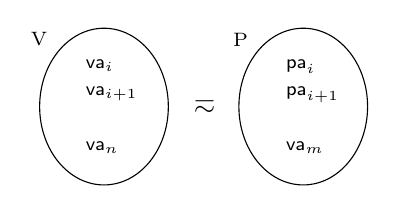
\begin{tikzpicture}[x=0.75pt,y=0.75pt,yscale=-0.5,xscale=0.5]
%uncomment if require: \path (0,176); %set diagram left start at 0, and has height of 176

%Shape: Ellipse [id:dp3089668103197505] 
\draw   (24,87.5) .. controls (24,45.8) and (51.76,12) .. (86,12) .. controls (120.24,12) and (148,45.8) .. (148,87.5) .. controls (148,129.2) and (120.24,163) .. (86,163) .. controls (51.76,163) and (24,129.2) .. (24,87.5) -- cycle ;
%Shape: Ellipse [id:dp3055465022453865] 
\draw   (216,87.5) .. controls (216,45.8) and (243.76,12) .. (278,12) .. controls (312.24,12) and (340,45.8) .. (340,87.5) .. controls (340,129.2) and (312.24,163) .. (278,163) .. controls (243.76,163) and (216,129.2) .. (216,87.5) -- cycle ;

% Text Node
\draw (13,13) node [anchor=north west][inner sep=0.75pt]   [align=left] {\scriptsize V};
% Text Node
\draw (208,14) node [anchor=north west][inner sep=0.75pt]   [align=left] {\scriptsize P};
% Text Node
\draw (170,79.4) node [anchor=north west][inner sep=0.75pt]    {$\eqsim $};
% Text Node
\draw (66,40) node [anchor=north west][inner sep=0.75pt]   [align=left] {\scriptsize $\mathsf{va}_i$};
% Text Node
\draw (66,66) node [anchor=north west][inner sep=0.75pt]   [align=left] {\scriptsize $\mathsf{va}_{i+1}$};
% Text Node
\draw (66,119) node [anchor=north west][inner sep=0.75pt]   [align=left] {\scriptsize $\mathsf{va}_n$};
% Text Node
\draw (259,40) node [anchor=north west][inner sep=0.75pt]   [align=left] {\scriptsize $\mathsf{pa}_i$};
% Text Node
\draw (259,66) node [anchor=north west][inner sep=0.75pt]   [align=left] {\scriptsize $\mathsf{pa}_{i+1}$};
% Text Node
\draw (259,119) node [anchor=north west][inner sep=0.75pt]   [align=left] {\scriptsize $\mathsf{va}_m$};


\end{tikzpicture}
       \caption{Virtualization: The Deception of Abundance}
       \label{fig:enter-label}
   \end{figure}
\end{frame}

%---------------------------------------------------
\begin{frame}[fragile]{Memory Location Virtualization: Abstraction}

  \begin{columns}[c] % The "c" option specifies centered vertical alignment while the "t" option is used for top vertical alignment

        \column{.45\textwidth} % Left column and width
        \textbf{An Address Space with Logical Name} $\gamma$
        \begin{figure}
    \centering
\tikzset{every picture/.style={line width=0.75pt}} %set default line width to 0.75pt        

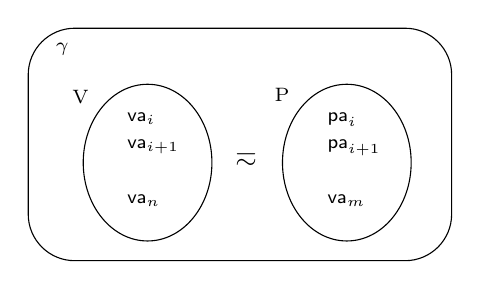
\begin{tikzpicture}[x=0.75pt,y=0.75pt,yscale=-0.5,xscale=0.5]
%uncomment if require: \path (0,250); %set diagram left start at 0, and has height of 250

%Shape: Ellipse [id:dp7871360559446556] 
\draw   (91,137.5) .. controls (91,95.8) and (118.76,62) .. (153,62) .. controls (187.24,62) and (215,95.8) .. (215,137.5) .. controls (215,179.2) and (187.24,213) .. (153,213) .. controls (118.76,213) and (91,179.2) .. (91,137.5) -- cycle ;
%Shape: Ellipse [id:dp9295032901075098] 
\draw   (283,137.5) .. controls (283,95.8) and (310.76,62) .. (345,62) .. controls (379.24,62) and (407,95.8) .. (407,137.5) .. controls (407,179.2) and (379.24,213) .. (345,213) .. controls (310.76,213) and (283,179.2) .. (283,137.5) -- cycle ;
%Rounded Rect [id:dp2598148010919421] 
\draw   (38,52.8) .. controls (38,28.06) and (58.06,8) .. (82.8,8) -- (401.2,8) .. controls (425.94,8) and (446,28.06) .. (446,52.8) -- (446,187.2) .. controls (446,211.94) and (425.94,232) .. (401.2,232) -- (82.8,232) .. controls (58.06,232) and (38,211.94) .. (38,187.2) -- cycle ;

% Text Node
\draw (78,65) node [anchor=north west][inner sep=0.75pt]   [align=left] {\scriptsize V};
% Text Node
\draw (273,63) node [anchor=north west][inner sep=0.75pt]   [align=left] {\scriptsize P};
% Text Node
\draw (235,126) node [anchor=north west][inner sep=0.75pt]    {$\eqsim $};
% Text Node
\draw (131,87) node [anchor=north west][inner sep=0.75pt]   [align=left] {\scriptsize $\mathsf{va}_i$};
% Text Node
\draw (131,113) node [anchor=north west][inner sep=0.75pt]   [align=left] {\scriptsize $\mathsf{va}_{i+1}$};
% Text Node
\draw (131,166) node [anchor=north west][inner sep=0.75pt]   [align=left] {\scriptsize $\mathsf{va}_n$};
% Text Node
\draw (324,87) node [anchor=north west][inner sep=0.75pt]   [align=left] {\scriptsize $\mathsf{pa}_i$};
% Text Node
\draw (324,113) node [anchor=north west][inner sep=0.75pt]   [align=left] {\scriptsize $\mathsf{pa}_{i+1}$};
% Text Node
\draw (324,166) node [anchor=north west][inner sep=0.75pt]   [align=left] {\scriptsize $\mathsf{va}_m$};
% Text Node
\draw (62,20) node [anchor=north west][inner sep=0.75pt]   [align=left] {\scriptsize $ \gamma $};


\end{tikzpicture}
   % In this slide, some important text will be \alert{highlighted} because it's important. Please, don't abuse it.

   % \begin{block}{Block}
   %     Sample text
   % \end{block}

%    \begin{alertblock}{Alertblock}
 %       Sample text in red box
 %   \end{alertblock}

  %  \begin{examples}
  %      Sample text in green box. The title of the block is ``Examples".
  %  \end{examples}
      \caption{Address-Spaces: Named Containers for Virtual Memory Mappings}
    \label{fig:enter-label}
\end{figure}

        \column{.45\textwidth} 
        \begin{columns}[c]
            \column{.55\textwidth}
            \textbf{A Program Named} $\gamma_n$
            \begin{lstlisting}[style=CStyleNum,mathescape]
    pointer va :=
     malloc(size)
\end{lstlisting}
            \column{.55\textwidth}
            \textbf{A Program Named} $\gamma_m$
            \begin{lstlisting}[style=CStyleNum,mathescape]
    pointer va := 
     malloc(size)
\end{lstlisting}
        \end{columns}
        \begin{itemize}
      \item  A program is abstracted as a \emph{named address-space}
      \item A container of \emph{virtual-to-physical} memory resource mappings
\end{itemize}
    \end{columns}
\end{frame}

%------------------------------------------------

\begin{frame}{Memory Location Virtualization: Mechanism}
\begin{figure}
    \centering

\tikzset{every picture/.style={line width=0.75pt}} %set default line width to 0.75pt        

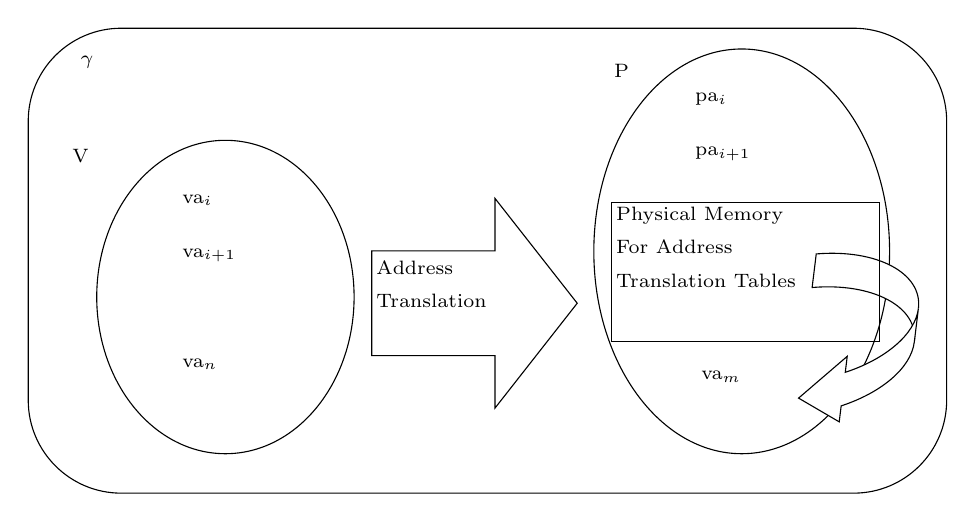
\begin{tikzpicture}[x=0.75pt,y=0.75pt,yscale=-1,xscale=1]
%uncomment if require: \path (0,250); %set diagram left start at 0, and has height of 250

%Shape: Ellipse [id:dp7871360559446556] 
\draw   (71,137.5) .. controls (71,95.8) and (98.76,62) .. (133,62) .. controls (167.24,62) and (195,95.8) .. (195,137.5) .. controls (195,179.2) and (167.24,213) .. (133,213) .. controls (98.76,213) and (71,179.2) .. (71,137.5) -- cycle ;
%Shape: Ellipse [id:dp9295032901075098] 
\draw   (310.5,115.5) .. controls (310.5,61.65) and (342.4,18) .. (381.75,18) .. controls (421.1,18) and (453,61.65) .. (453,115.5) .. controls (453,169.35) and (421.1,213) .. (381.75,213) .. controls (342.4,213) and (310.5,169.35) .. (310.5,115.5) -- cycle ;
%Rounded Rect [id:dp2598148010919421] 
\draw   (38,52.8) .. controls (38,28.06) and (58.06,8) .. (82.8,8) -- (435.7,8) .. controls (460.44,8) and (480.5,28.06) .. (480.5,52.8) -- (480.5,187.2) .. controls (480.5,211.94) and (460.44,232) .. (435.7,232) -- (82.8,232) .. controls (58.06,232) and (38,211.94) .. (38,187.2) -- cycle ;
%Right Arrow [id:dp17531291394449267] 
\draw   (203.5,115.25) -- (262.9,115.25) -- (262.9,90) -- (302.5,140.5) -- (262.9,191) -- (262.9,165.75) -- (203.5,165.75) -- cycle ;
%Curve Right Arrow [id:dp08259202048956893] 
\draw  [fill={rgb, 255:red, 255; green, 255; blue, 255 }  ,fill opacity=1 ] (464.91,159.13) .. controls (466.98,142.19) and (444.94,130.45) .. (415.68,132.92) -- (417.66,116.75) .. controls (446.92,114.27) and (468.96,126.01) .. (466.89,142.96) ;\draw  [fill={rgb, 255:red, 255; green, 255; blue, 255 }  ,fill opacity=1 ] (466.89,142.96) .. controls (465.35,155.54) and (450.94,167.46) .. (431.65,173.78) -- (432.59,166.08) -- (409.15,186.21) -- (428.73,197.65) -- (429.67,189.95) .. controls (448.96,183.64) and (463.37,171.72) .. (464.91,159.13)(466.89,142.96) -- (464.91,159.13) ;

% Text Node
\draw (58,65) node [anchor=north west][inner sep=0.75pt]   [align=left] {\scriptsize V};
% Text Node
\draw (319,24) node [anchor=north west][inner sep=0.75pt]   [align=left] {\scriptsize P};
% Text Node
\draw (111,87) node [anchor=north west][inner sep=0.75pt]   [align=left] {\scriptsize va$_i$};
% Text Node
\draw (111,113) node [anchor=north west][inner sep=0.75pt]   [align=left] {\scriptsize va$_{i+1}$};
% Text Node
\draw (111,166) node [anchor=north west][inner sep=0.75pt]   [align=left] {\scriptsize va$_n$};
% Text Node
\draw (358,38) node [anchor=north west][inner sep=0.75pt]   [align=left] {\scriptsize pa$_i$};
% Text Node
\draw (358,64) node [anchor=north west][inner sep=0.75pt]   [align=left] {\scriptsize pa$_{i+1}$};
% Text Node
\draw (361,172) node [anchor=north west][inner sep=0.75pt]   [align=left] {\scriptsize va$_m$};
% Text Node
\draw (62,20) node [anchor=north west][inner sep=0.75pt]   [align=left] {\scriptsize $\gamma $};
% Text Node
\draw (204.5,119) node [anchor=north west][inner sep=0.75pt]   [align=left] {\scriptsize Address\\ \scriptsize Translation};
% Text Node
\draw    (319,92) -- (448,92) -- (448,159) -- (319,159) -- cycle  ;
\draw (320,93) node [anchor=north west][inner sep=0.75pt]   [align=left] {\scriptsize Physical Memory\\ \scriptsize For Address \\ \scriptsize Translation Tables};


\end{tikzpicture}
    \caption{Address-Translation: A Mechanism for Realizing Address Virtualization}
    \label{fig:enter-label}
\end{figure}

\end{frame}

%------------------------------------------------

\begin{frame}{Page Tables}
  

\begin{figure}
    \centering



\tikzset{every picture/.style={line width=0.75pt}} %set default line width to 0.75pt        

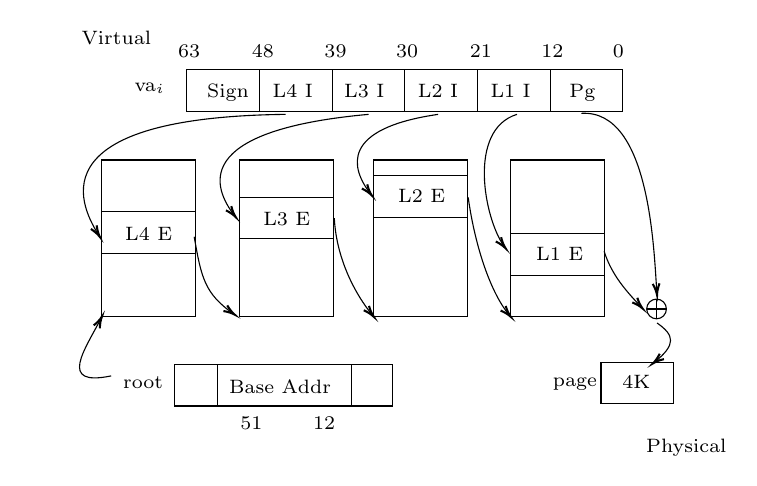
\begin{tikzpicture}[x=0.75pt,y=0.75pt,yscale=-0.5,xscale=0.5]
%uncomment if require: \path (0,444); %set diagram left start at 0, and has height of 444

%Shape: Rectangle [id:dp9406932326447903] 
\draw   (33,141) -- (123,141) -- (123,292) -- (33,292) -- cycle ;
%Shape: Rectangle [id:dp7682116051394419] 
\draw   (166,141) -- (256,141) -- (256,292) -- (166,292) -- cycle ;
%Shape: Rectangle [id:dp07376733516930423] 
\draw   (295,141) -- (385,141) -- (385,292) -- (295,292) -- cycle ;
%Shape: Rectangle [id:dp7106629147891306] 
\draw   (427,141) -- (517,141) -- (517,292) -- (427,292) -- cycle ;
%Shape: Rectangle [id:dp1342906826203598] 
\draw   (115,54) -- (185,54) -- (185,94) -- (115,94) -- cycle ;
%Shape: Rectangle [id:dp08072439007207399] 
\draw   (185,54) -- (255,54) -- (255,94) -- (185,94) -- cycle ;
%Shape: Rectangle [id:dp8282933603833216] 
\draw   (255,54) -- (325,54) -- (325,94) -- (255,94) -- cycle ;
%Shape: Rectangle [id:dp8416255090865326] 
\draw   (325,54) -- (395,54) -- (395,94) -- (325,94) -- cycle ;
%Shape: Rectangle [id:dp22911958218529804] 
\draw   (395,54) -- (465,54) -- (465,94) -- (395,94) -- cycle ;
%Shape: Rectangle [id:dp33732955213990756] 
\draw   (465,54) -- (535,54) -- (535,94) -- (465,94) -- cycle ;
%Curve Lines [id:da6688730321284677] 
\draw    (210,97) .. controls (-37.94,99.94) and (15.69,190.28) .. (30.17,213.65) ;
\draw [shift={(31,215)}, rotate = 238.24] [color={rgb, 255:red, 0; green, 0; blue, 0 }  ][line width=0.75]    (10.93,-3.29) .. controls (6.95,-1.4) and (3.31,-0.3) .. (0,0) .. controls (3.31,0.3) and (6.95,1.4) .. (10.93,3.29)   ;
%Shape: Rectangle [id:dp6044747978986409] 
\draw   (33,191) -- (123,191) -- (123,231) -- (33,231) -- cycle ;
%Curve Lines [id:da8867562998134584] 
\draw    (290,97) .. controls (116.54,112.68) and (140.92,168.7) .. (160.79,194.46) ;
\draw [shift={(162,196)}, rotate = 231.34] [color={rgb, 255:red, 0; green, 0; blue, 0 }  ][line width=0.75]    (10.93,-3.29) .. controls (6.95,-1.4) and (3.31,-0.3) .. (0,0) .. controls (3.31,0.3) and (6.95,1.4) .. (10.93,3.29)   ;
%Shape: Rectangle [id:dp8861153167245819] 
\draw   (166,177) -- (256,177) -- (256,217) -- (166,217) -- cycle ;
%Shape: Rectangle [id:dp05979844200848894] 
\draw   (295,156) -- (385,156) -- (385,196) -- (295,196) -- cycle ;
%Shape: Rectangle [id:dp17403733244247843] 
\draw   (427,212) -- (517,212) -- (517,252) -- (427,252) -- cycle ;
%Curve Lines [id:da20581124900573955] 
\draw    (357,97) .. controls (262.92,110.72) and (272.56,148.45) .. (291.81,173.48) ;
\draw [shift={(293,175)}, rotate = 231.34] [color={rgb, 255:red, 0; green, 0; blue, 0 }  ][line width=0.75]    (10.93,-3.29) .. controls (6.95,-1.4) and (3.31,-0.3) .. (0,0) .. controls (3.31,0.3) and (6.95,1.4) .. (10.93,3.29)   ;
%Curve Lines [id:da07589611603635316] 
\draw    (433,97) .. controls (384.98,111.7) and (401.31,197.47) .. (420.8,224.42) ;
\draw [shift={(422,226)}, rotate = 231.34] [color={rgb, 255:red, 0; green, 0; blue, 0 }  ][line width=0.75]    (10.93,-3.29) .. controls (6.95,-1.4) and (3.31,-0.3) .. (0,0) .. controls (3.31,0.3) and (6.95,1.4) .. (10.93,3.29)   ;
%Curve Lines [id:da6852167546673456] 
\draw    (495,96) .. controls (561.98,92.06) and (564.93,230.74) .. (567.87,269.31) ;
\draw [shift={(568,271)}, rotate = 265.24] [color={rgb, 255:red, 0; green, 0; blue, 0 }  ][line width=0.75]    (10.93,-3.29) .. controls (6.95,-1.4) and (3.31,-0.3) .. (0,0) .. controls (3.31,0.3) and (6.95,1.4) .. (10.93,3.29)   ;
%Curve Lines [id:da017521077423665377] 
\draw    (42,349) .. controls (-10.21,359.84) and (17.15,323.13) .. (32.32,293.36) ;
\draw [shift={(33,292)}, rotate = 116.57] [color={rgb, 255:red, 0; green, 0; blue, 0 }  ][line width=0.75]    (10.93,-3.29) .. controls (6.95,-1.4) and (3.31,-0.3) .. (0,0) .. controls (3.31,0.3) and (6.95,1.4) .. (10.93,3.29)   ;
%Curve Lines [id:da6750042432035159] 
\draw    (122,215) .. controls (128.9,254.4) and (131.91,269.54) .. (159.71,289.1) ;
\draw [shift={(161,290)}, rotate = 214.59] [color={rgb, 255:red, 0; green, 0; blue, 0 }  ][line width=0.75]    (10.93,-3.29) .. controls (6.95,-1.4) and (3.31,-0.3) .. (0,0) .. controls (3.31,0.3) and (6.95,1.4) .. (10.93,3.29)   ;
%Curve Lines [id:da14788158682113428] 
\draw    (257,197) .. controls (258.95,236) and (277.06,270.25) .. (293.72,290.47) ;
\draw [shift={(295,292)}, rotate = 229.64] [color={rgb, 255:red, 0; green, 0; blue, 0 }  ][line width=0.75]    (10.93,-3.29) .. controls (6.95,-1.4) and (3.31,-0.3) .. (0,0) .. controls (3.31,0.3) and (6.95,1.4) .. (10.93,3.29)   ;
%Curve Lines [id:da3297977595767969] 
\draw    (386,177) .. controls (392.86,226) and (408.36,270.2) .. (425.92,290.77) ;
\draw [shift={(427,292)}, rotate = 228.01] [color={rgb, 255:red, 0; green, 0; blue, 0 }  ][line width=0.75]    (10.93,-3.29) .. controls (6.95,-1.4) and (3.31,-0.3) .. (0,0) .. controls (3.31,0.3) and (6.95,1.4) .. (10.93,3.29)   ;
%Curve Lines [id:da7710391961792686] 
\draw    (517,229) .. controls (524.76,253.25) and (540.05,269.03) .. (552.82,282.73) ;
\draw [shift={(554,284)}, rotate = 227.12] [color={rgb, 255:red, 0; green, 0; blue, 0 }  ][line width=0.75]    (10.93,-3.29) .. controls (6.95,-1.4) and (3.31,-0.3) .. (0,0) .. controls (3.31,0.3) and (6.95,1.4) .. (10.93,3.29)   ;
%Shape: Rectangle [id:dp1535611125971872] 
\draw   (514,336) -- (584,336) -- (584,376) -- (514,376) -- cycle ;
%Shape: Rectangle [id:dp05427947476226991] 
\draw   (103,338) -- (144.5,338) -- (144.5,378) -- (103,378) -- cycle ;
%Shape: Rectangle [id:dp10511138743752002] 
\draw   (144.5,338) -- (273.5,338) -- (273.5,378) -- (144.5,378) -- cycle ;
%Shape: Rectangle [id:dp8917680919534263] 
\draw   (273.5,338) -- (313,338) -- (313,378) -- (273.5,378) -- cycle ;
\draw   (558,284.5) .. controls (558,279.25) and (562.25,275) .. (567.5,275) .. controls (572.75,275) and (577,279.25) .. (577,284.5) .. controls (577,289.75) and (572.75,294) .. (567.5,294) .. controls (562.25,294) and (558,289.75) .. (558,284.5) -- cycle ; \draw   (558,284.5) -- (577,284.5) ; \draw   (567.5,275) -- (567.5,294) ;
%Curve Lines [id:da9312068388962929] 
\draw    (568,298) .. controls (584.66,309.76) and (586.91,318.64) .. (565.35,335.93) ;
\draw [shift={(564,337)}, rotate = 321.95] [color={rgb, 255:red, 0; green, 0; blue, 0 }  ][line width=0.75]    (10.93,-3.29) .. controls (6.95,-1.4) and (3.31,-0.3) .. (0,0) .. controls (3.31,0.3) and (6.95,1.4) .. (10.93,3.29)   ;

% Text Node
\draw (11,14) node [anchor=north west][inner sep=0.75pt]   [align=left] {{\scriptsize Virtual}};
% Text Node
\draw (555,407) node [anchor=north west][inner sep=0.75pt]   [align=left] {{\scriptsize Physical}};
% Text Node
\draw (104,28) node [anchor=north west][inner sep=0.75pt]   [align=left] {{\scriptsize 63}};
% Text Node
\draw (175,28) node [anchor=north west][inner sep=0.75pt]   [align=left] {{\scriptsize 48}};
% Text Node
\draw (245,28) node [anchor=north west][inner sep=0.75pt]   [align=left] {{\scriptsize 39}};
% Text Node
\draw (314,28) node [anchor=north west][inner sep=0.75pt]   [align=left] {{\scriptsize 30}};
% Text Node
\draw (385,28) node [anchor=north west][inner sep=0.75pt]   [align=left] {{\scriptsize 21}};
% Text Node
\draw (454,28) node [anchor=north west][inner sep=0.75pt]   [align=left] {{\scriptsize 12}};
% Text Node
\draw (523,28) node [anchor=north west][inner sep=0.75pt]   [align=left] {{\scriptsize 0}};
% Text Node
\draw (132,65) node [anchor=north west][inner sep=0.75pt]   [align=left] {{\scriptsize Sign}};
% Text Node
\draw (195,65) node [anchor=north west][inner sep=0.75pt]   [align=left] {{\scriptsize L4 I}};
% Text Node
\draw (264,65) node [anchor=north west][inner sep=0.75pt]   [align=left] {{\scriptsize L3 I}};
% Text Node
\draw (335,65) node [anchor=north west][inner sep=0.75pt]   [align=left] {{\scriptsize L2 I}};
% Text Node
\draw (405,65) node [anchor=north west][inner sep=0.75pt]   [align=left] {{\scriptsize L1 I}};
% Text Node
\draw (481,65) node [anchor=north west][inner sep=0.75pt]   [align=left] {{\scriptsize Pg}};
% Text Node
\draw (62,64) node [anchor=north west][inner sep=0.75pt]   [align=left] {{\scriptsize va$_i$}};
% Text Node
\draw (53,203) node [anchor=north west][inner sep=0.75pt]   [align=left] {{\scriptsize L4 E}};
% Text Node
\draw (186,189) node [anchor=north west][inner sep=0.75pt]   [align=left] {{\scriptsize L3 E}};
% Text Node
\draw (316,167) node [anchor=north west][inner sep=0.75pt]   [align=left] {{\scriptsize L2 E}};
% Text Node
\draw (449,223) node [anchor=north west][inner sep=0.75pt]   [align=left] {{\scriptsize L1 E}};
% Text Node
\draw (51,347) node [anchor=north west][inner sep=0.75pt]   [align=left] {{\scriptsize root}};
% Text Node
\draw (465,349) node [anchor=north west][inner sep=0.75pt]   [align=left] {{\scriptsize page}};
% Text Node
\draw (532,346) node [anchor=north west][inner sep=0.75pt]   [align=left] {{\scriptsize 4K}};
% Text Node
\draw (164,386) node [anchor=north west][inner sep=0.75pt]   [align=left] {{\scriptsize 51}};
% Text Node
\draw (234,386) node [anchor=north west][inner sep=0.75pt]   [align=left] {{\scriptsize 12}};
% Text Node
\draw (153,350) node [anchor=north west][inner sep=0.75pt]   [align=left] {{\scriptsize Base Addr}};


\end{tikzpicture}
    \caption{Page-Tables (\textbf{PT}): Data Structures for Address-Translation}
    \label{fig:enter-label}
\end{figure}
\end{frame}

%------------------------------------------------
\begin{frame}{A Complete Picture of Address-Space Abstraction}
\begin{columns}[c]
\column{.35\textwidth}    
\begin{figure}
    \centering
    


\tikzset{every picture/.style={line width=0.75pt}} %set default line width to 0.75pt        

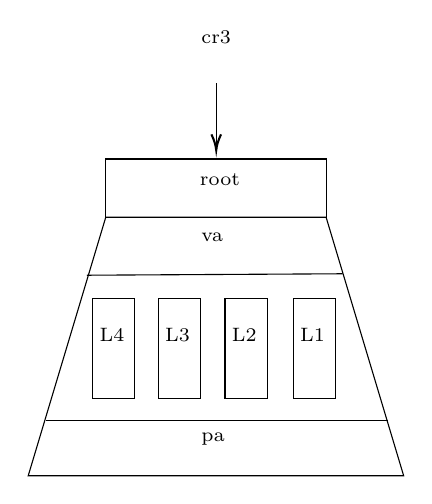
\begin{tikzpicture}[x=0.75pt,y=0.75pt,yscale=-0.7,xscale=0.7]
%uncomment if require: \path (0,361); %set diagram left start at 0, and has height of 361

%Straight Lines [id:da9421316390034546] 
\draw    (150,49) -- (150,93) ;
\draw [shift={(150,95)}, rotate = 270] [color={rgb, 255:red, 0; green, 0; blue, 0 }  ][line width=0.75]    (10.93,-3.29) .. controls (6.95,-1.4) and (3.31,-0.3) .. (0,0) .. controls (3.31,0.3) and (6.95,1.4) .. (10.93,3.29)   ;
%Shape: Trapezoid [id:dp42196090147818355] 
\draw   (20.6,319) -- (74,141) -- (225.6,141) -- (279,319) -- cycle ;
%Shape: Rectangle [id:dp05833798878152763] 
\draw   (74,101) -- (226,101) -- (226,141) -- (74,141) -- cycle ;
%Straight Lines [id:da5475026726551153] 
\draw    (61,181) -- (237,180) ;
%Straight Lines [id:da567347542499933] 
\draw    (33,281) -- (268,281) ;
%Shape: Rectangle [id:dp8593208287745469] 
\draw   (65,197) -- (94,197) -- (94,266) -- (65,266) -- cycle ;
%Shape: Rectangle [id:dp07187149088731903] 
\draw   (110,197) -- (139,197) -- (139,266) -- (110,266) -- cycle ;
%Shape: Rectangle [id:dp13017365116217516] 
\draw   (156,197) -- (185,197) -- (185,266) -- (156,266) -- cycle ;
%Shape: Rectangle [id:dp8238066656621155] 
\draw   (203,197) -- (232,197) -- (232,266) -- (203,266) -- cycle ;

% Text Node
\draw (138,11) node [anchor=north west][inner sep=0.75pt]   [align=left] {{\scriptsize cr3}};
% Text Node
\draw (138,150) node [anchor=north west][inner sep=0.75pt]   [align=left] {{\scriptsize va}};
% Text Node
\draw (138,288) node [anchor=north west][inner sep=0.75pt]   [align=left] {{\scriptsize pa}};
% Text Node
\draw (68,216) node [anchor=north west][inner sep=0.75pt]   [align=left] {{\scriptsize L4}};
% Text Node
\draw (113,216) node [anchor=north west][inner sep=0.75pt]   [align=left] {{\scriptsize L3}};
% Text Node
\draw (159,216) node [anchor=north west][inner sep=0.75pt]   [align=left] {{\scriptsize L2}};
% Text Node
\draw (206,216) node [anchor=north west][inner sep=0.75pt]   [align=left] {{\scriptsize L1}};
% Text Node
\draw (137,109) node [anchor=north west][inner sep=0.75pt]   [align=left] {{\scriptsize root}};


\end{tikzpicture}
    \caption{Depicting an Address-Space with its Essential Aspects}
    \label{fig:enter-label}
\end{figure}
\column{.6\textwidth}
  \begin{block}{The Current View of Memory}
    The register $\mathsf{cr}_3$ points to the current view of the memory, i.e., the loaded address space in the memory \end{block}.
\end{columns}

\end{frame}

\section{Motivation}
\begin{frame}{Virtual Memory Management (\textbf{VMM})}
    \begin{block}{\textbf{VMM} as a General Resource Provider}
    "the virtual memory sub-system can be considered the core of a Solaris instance, and the implementation of Solaris virtual memory affects just about every other subsystem in the operating system" \cite{mcdougall2006solaris}
    \end{block}
\end{frame}

%------------------------------------------------
\subsection{Sharing}

%Sharing Physical Page Tables 
%1.------------------------------------------------
\begin{frame}{Sharing Physical Page Tables}
    \begin{figure}
        \centering
        


\tikzset{every picture/.style={line width=0.75pt}} %set default line width to 0.75pt        

\begin{tikzpicture}[x=0.75pt,y=0.75pt,yscale=-0.5,xscale=0.5]
%uncomment if require: \path (0,438); %set diagram left start at 0, and has height of 438

%Shape: Rectangle [id:dp7317880523817719] 
\draw   (118,55) -- (188,55) -- (188,95) -- (118,95) -- cycle ;
%Shape: Rectangle [id:dp5225486463875249] 
\draw   (188,55) -- (258,55) -- (258,95) -- (188,95) -- cycle ;
%Shape: Rectangle [id:dp286436732742432] 
\draw   (258,55) -- (328,55) -- (328,95) -- (258,95) -- cycle ;
%Shape: Rectangle [id:dp23476266141975666] 
\draw   (328,55) -- (398,55) -- (398,95) -- (328,95) -- cycle ;
%Shape: Rectangle [id:dp20898213992300274] 
\draw   (398,55) -- (468,55) -- (468,95) -- (398,95) -- cycle ;
%Shape: Rectangle [id:dp347367086236243] 
\draw   (468,55) -- (538,55) -- (538,95) -- (468,95) -- cycle ;
%Shape: Rectangle [id:dp44942702288840586] 
\draw   (81,339) -- (122.5,339) -- (122.5,379) -- (81,379) -- cycle ;
%Shape: Rectangle [id:dp47453526528917545] 
\draw   (122.5,339) -- (251.5,339) -- (251.5,379) -- (122.5,379) -- cycle ;
%Shape: Rectangle [id:dp7167826579126793] 
\draw   (251.5,339) -- (291,339) -- (291,379) -- (251.5,379) -- cycle ;
%Shape: Rectangle [id:dp2025452842323363] 
\draw   (521,339) -- (591,339) -- (591,379) -- (521,379) -- cycle ;

% Text Node
\draw (14,15) node [anchor=north west][inner sep=0.75pt]   [align=left] {{\scriptsize Virtual}};
% Text Node
\draw (589,410) node [anchor=north west][inner sep=0.75pt]   [align=left] {{\scriptsize Physical}};
% Text Node
\draw (142,387) node [anchor=north west][inner sep=0.75pt]   [align=left] {{\scriptsize 51}};
% Text Node
\draw (212,387) node [anchor=north west][inner sep=0.75pt]   [align=left] {{\scriptsize 12}};
% Text Node
\draw (107,29) node [anchor=north west][inner sep=0.75pt]   [align=left] {{\scriptsize 63}};
% Text Node
\draw (178,29) node [anchor=north west][inner sep=0.75pt]   [align=left] {{\scriptsize 48}};
% Text Node
\draw (248,29) node [anchor=north west][inner sep=0.75pt]   [align=left] {{\scriptsize 39}};
% Text Node
\draw (317,29) node [anchor=north west][inner sep=0.75pt]   [align=left] {{\scriptsize 30}};
% Text Node
\draw (388,29) node [anchor=north west][inner sep=0.75pt]   [align=left] {{\scriptsize 21}};
% Text Node
\draw (457,29) node [anchor=north west][inner sep=0.75pt]   [align=left] {{\scriptsize 12}};
% Text Node
\draw (526,29) node [anchor=north west][inner sep=0.75pt]   [align=left] {{\scriptsize 0}};
% Text Node
\draw (135,66) node [anchor=north west][inner sep=0.75pt]   [align=left] {{\scriptsize Sign}};
% Text Node
\draw (198,66) node [anchor=north west][inner sep=0.75pt]   [align=left] {{\scriptsize L4 I}};
% Text Node
\draw (267,65) node [anchor=north west][inner sep=0.75pt]   [align=left] {{\scriptsize L3 I}};
% Text Node
\draw (338,65) node [anchor=north west][inner sep=0.75pt]   [align=left] {{\scriptsize L2 I}};
% Text Node
\draw (408,66) node [anchor=north west][inner sep=0.75pt]   [align=left] {{\scriptsize L1 I}};
% Text Node
\draw (484,66) node [anchor=north west][inner sep=0.75pt]   [align=left] {{\scriptsize Pg}};
% Text Node
\draw (61,64) node [anchor=north west][inner sep=0.75pt]   [align=left] {{\scriptsize va$_i$}};
% Text Node
\draw (25,350) node [anchor=north west][inner sep=0.75pt]   [align=left] {{\scriptsize root}};
% Text Node
\draw (459,350) node [anchor=north west][inner sep=0.75pt]   [align=left] {{\scriptsize page}};
% Text Node
\draw (539,349) node [anchor=north west][inner sep=0.75pt]   [align=left] {{\scriptsize 4K}};
% Text Node
\draw (131,351) node [anchor=north west][inner sep=0.75pt]   [align=left] {{\scriptsize Base Addr}};


\end{tikzpicture}
        \caption{Physical and Virtual Resources}
        \label{fig:enter-label}
    \end{figure}
\end{frame}
%Sharing Physical Page Tables
%2--------------------------------------------------
\begin{frame}[fragile]{Sharing Physical Page Tables}
\begin{columns}[c]
\column{.59\textwidth}    
    \begin{figure}
        \centering



\tikzset{every picture/.style={line width=0.75pt}} %set default line width to 0.75pt        

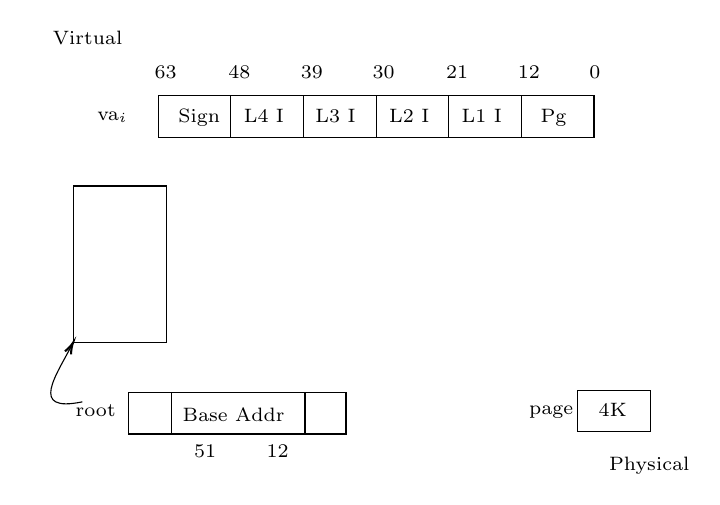
\begin{tikzpicture}[x=0.75pt,y=0.75pt,yscale=-0.5,xscale=0.5]
%uncomment if require: \path (0,458); %set diagram left start at 0, and has height of 458

%Shape: Rectangle [id:dp20969678453076424] 
\draw   (37,167) -- (127,167) -- (127,318) -- (37,318) -- cycle ;
%Shape: Rectangle [id:dp004275189078232211] 
\draw   (119,80) -- (189,80) -- (189,120) -- (119,120) -- cycle ;
%Shape: Rectangle [id:dp3335681417124716] 
\draw   (189,80) -- (259,80) -- (259,120) -- (189,120) -- cycle ;
%Shape: Rectangle [id:dp251303061085524] 
\draw   (259,80) -- (329,80) -- (329,120) -- (259,120) -- cycle ;
%Shape: Rectangle [id:dp970404754682167] 
\draw   (329,80) -- (399,80) -- (399,120) -- (329,120) -- cycle ;
%Shape: Rectangle [id:dp04891415906042229] 
\draw   (399,80) -- (469,80) -- (469,120) -- (399,120) -- cycle ;
%Shape: Rectangle [id:dp4593533880279508] 
\draw   (469,80) -- (539,80) -- (539,120) -- (469,120) -- cycle ;
%Curve Lines [id:da28481454982934795] 
\draw    (46,375) .. controls (-6.21,385.84) and (21.15,349.13) .. (36.32,319.36) ;
\draw [shift={(37,318)}, rotate = 116.57] [color={rgb, 255:red, 0; green, 0; blue, 0 }  ][line width=0.75]    (10.93,-3.29) .. controls (6.95,-1.4) and (3.31,-0.3) .. (0,0) .. controls (3.31,0.3) and (6.95,1.4) .. (10.93,3.29)   ;
%Shape: Rectangle [id:dp6340955170231213] 
\draw   (523,364) -- (593,364) -- (593,404) -- (523,404) -- cycle ;
%Shape: Rectangle [id:dp027002563853506523] 
\draw   (90,366) -- (131.5,366) -- (131.5,406) -- (90,406) -- cycle ;
%Shape: Rectangle [id:dp4636490131021511] 
\draw   (131.5,366) -- (260.5,366) -- (260.5,406) -- (131.5,406) -- cycle ;
%Shape: Rectangle [id:dp09160630738854891] 
\draw   (260.5,366) -- (300,366) -- (300,406) -- (260.5,406) -- cycle ;

% Text Node
\draw (15,15) node [anchor=north west][inner sep=0.75pt]   [align=left] {{\scriptsize Virtual}};
% Text Node
\draw (551,426) node [anchor=north west][inner sep=0.75pt]   [align=left] {{\scriptsize Physical}};
% Text Node
\draw (136,91) node [anchor=north west][inner sep=0.75pt]   [align=left] {{\scriptsize Sign}};
% Text Node
\draw (199,91) node [anchor=north west][inner sep=0.75pt]   [align=left] {{\scriptsize L4 I}};
% Text Node
\draw (268,91) node [anchor=north west][inner sep=0.75pt]   [align=left] {{\scriptsize L3 I}};
% Text Node
\draw (339,91) node [anchor=north west][inner sep=0.75pt]   [align=left] {{\scriptsize L2 I}};
% Text Node
\draw (409,91) node [anchor=north west][inner sep=0.75pt]   [align=left] {{\scriptsize L1 I}};
% Text Node
\draw (485,91) node [anchor=north west][inner sep=0.75pt]   [align=left] {{\scriptsize Pg}};
% Text Node
\draw (58,93) node [anchor=north west][inner sep=0.75pt]   [align=left] {{\scriptsize va$_i$}};
% Text Node
\draw (37,375) node [anchor=north west][inner sep=0.75pt]   [align=left] {{\scriptsize root}};
% Text Node
\draw (474,377) node [anchor=north west][inner sep=0.75pt]   [align=left] {{\scriptsize page}};
% Text Node
\draw (541,374) node [anchor=north west][inner sep=0.75pt]   [align=left] {{\scriptsize 4K}};
% Text Node
\draw (151,414) node [anchor=north west][inner sep=0.75pt]   [align=left] {{\scriptsize 51}};
% Text Node
\draw (221,414) node [anchor=north west][inner sep=0.75pt]   [align=left] {{\scriptsize 12}};
% Text Node
\draw (140,378) node [anchor=north west][inner sep=0.75pt]   [align=left] {{\scriptsize Base Addr}};
% Text Node
\draw (113,49) node [anchor=north west][inner sep=0.75pt]   [align=left] {{\scriptsize 63}};
% Text Node
\draw (184,49) node [anchor=north west][inner sep=0.75pt]   [align=left] {{\scriptsize 48}};
% Text Node
\draw (254,49) node [anchor=north west][inner sep=0.75pt]   [align=left] {{\scriptsize 39}};
% Text Node
\draw (323,49) node [anchor=north west][inner sep=0.75pt]   [align=left] {{\scriptsize 30}};
% Text Node
\draw (394,49) node [anchor=north west][inner sep=0.75pt]   [align=left] {{\scriptsize 21}};
% Text Node
\draw (463,49) node [anchor=north west][inner sep=0.75pt]   [align=left] {{\scriptsize 12}};
% Text Node
\draw (532,49) node [anchor=north west][inner sep=0.75pt]   [align=left] {{\scriptsize 0}};


\end{tikzpicture}
        \caption{Traversal Starts from the \textsf{root}}
        \label{fig:enter-label}
    \end{figure}
    \column{.4\textwidth}
\begin{lstlisting}[style=CStyleNum, basicstyle=\tiny]
static pte_t *pte_nxt_table (pte_t *entry){
 pte_t *next;
 // If not already present, try to allocate
 if (!entry->present){
  if (!pte_alloc(&next)) {
   return NULL;
  }
  entry->pfn = PTE_PFN((uintptr_t) next);
  entry->present = 1;
  } else {
   uintptr_t next_phys_addr = PTE_PFN_TO_ADDR(entry->pfn);        
   uintptr_t next_virt_addr = (uintptr_t) P2V(next_phys_addr);
   next = (pte_t *) next_virt_addr;
  }
  return next;
}   
pte_t *walkpgdir(pte_t *l4, void *va){ 
\end{lstlisting}
\end{columns}
\end{frame}
%3--------------------------------------------------
\begin{frame}[fragile]{Sharing Physical Page Tables}
\begin{columns}[c]
\column{.59\textwidth}    
    \begin{figure}
        \centering

\tikzset{every picture/.style={line width=0.75pt}} %set default line width to 0.75pt        

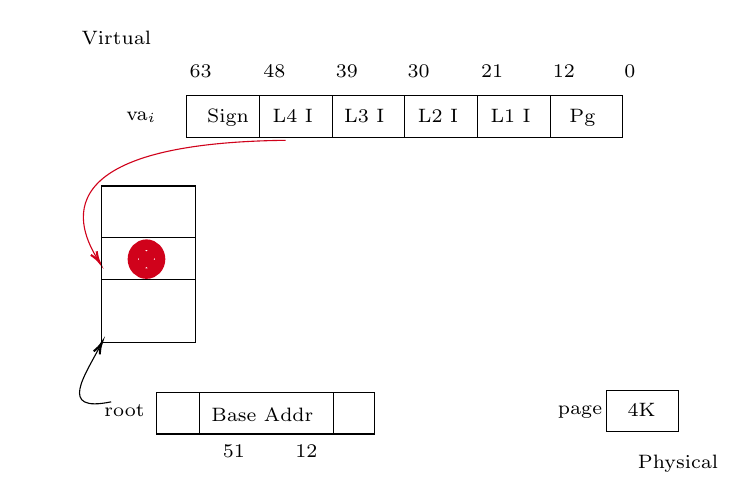
\begin{tikzpicture}[x=0.75pt,y=0.75pt,yscale=-0.5,xscale=0.5]
%uncomment if require: \path (0,463); %set diagram left start at 0, and has height of 463

%Shape: Rectangle [id:dp22823252469987754] 
\draw   (33,168) -- (123,168) -- (123,319) -- (33,319) -- cycle ;
%Shape: Rectangle [id:dp38643603035450225] 
\draw   (115,81) -- (185,81) -- (185,121) -- (115,121) -- cycle ;
%Shape: Rectangle [id:dp930520023551549] 
\draw   (185,81) -- (255,81) -- (255,121) -- (185,121) -- cycle ;
%Shape: Rectangle [id:dp7714286193511939] 
\draw   (255,81) -- (325,81) -- (325,121) -- (255,121) -- cycle ;
%Shape: Rectangle [id:dp7050983457803661] 
\draw   (325,81) -- (395,81) -- (395,121) -- (325,121) -- cycle ;
%Shape: Rectangle [id:dp05967324913136096] 
\draw   (395,81) -- (465,81) -- (465,121) -- (395,121) -- cycle ;
%Shape: Rectangle [id:dp45157167705022294] 
\draw   (465,81) -- (535,81) -- (535,121) -- (465,121) -- cycle ;
%Curve Lines [id:da23509576960998113] 
\draw [color={rgb, 255:red, 208; green, 2; blue, 27 }  ,draw opacity=1 ]   (210,124) .. controls (-37.94,126.94) and (15.69,217.28) .. (30.17,240.65) ;
\draw [shift={(31,242)}, rotate = 238.24] [color={rgb, 255:red, 208; green, 2; blue, 27 }  ,draw opacity=1 ][line width=0.75]    (10.93,-3.29) .. controls (6.95,-1.4) and (3.31,-0.3) .. (0,0) .. controls (3.31,0.3) and (6.95,1.4) .. (10.93,3.29)   ;
%Shape: Rectangle [id:dp4213782718477044] 
\draw   (33,218) -- (123,218) -- (123,258) -- (33,258) -- cycle ;
%Curve Lines [id:da06682709181758373] 
\draw    (42,376) .. controls (-10.21,386.84) and (17.15,350.13) .. (32.32,320.36) ;
\draw [shift={(33,319)}, rotate = 116.57] [color={rgb, 255:red, 0; green, 0; blue, 0 }  ][line width=0.75]    (10.93,-3.29) .. controls (6.95,-1.4) and (3.31,-0.3) .. (0,0) .. controls (3.31,0.3) and (6.95,1.4) .. (10.93,3.29)   ;
%Shape: Rectangle [id:dp07658260006827389] 
\draw   (519,365) -- (589,365) -- (589,405) -- (519,405) -- cycle ;
%Shape: Rectangle [id:dp1865179749417738] 
\draw   (86,367) -- (127.5,367) -- (127.5,407) -- (86,407) -- cycle ;
%Shape: Rectangle [id:dp10111488671096569] 
\draw   (127.5,367) -- (256.5,367) -- (256.5,407) -- (127.5,407) -- cycle ;
%Shape: Rectangle [id:dp8897733490834594] 
\draw   (256.5,367) -- (296,367) -- (296,407) -- (256.5,407) -- cycle ;
%Shape: Light Bulb [id:dp6972254317722191] 
\draw  [color={rgb, 255:red, 208; green, 2; blue, 27 }  ,draw opacity=1 ][line width=3.75]  (62.88,238.5) .. controls (62.88,230.77) and (68.75,224.5) .. (76,224.5) .. controls (83.25,224.5) and (89.13,230.77) .. (89.13,238.5) .. controls (89.13,246.23) and (83.25,252.5) .. (76,252.5) .. controls (68.75,252.5) and (62.88,246.23) .. (62.88,238.5) -- cycle (66.66,228.53) -- (85.35,248.47) (85.35,228.53) -- (66.66,248.47) (60.25,238.5) -- (62.88,238.5) (89.13,238.5) -- (91.75,238.5) ;

% Text Node
\draw (11,16) node [anchor=north west][inner sep=0.75pt]   [align=left] {{\scriptsize Virtual}};
% Text Node
\draw (547,425) node [anchor=north west][inner sep=0.75pt]   [align=left] {{\scriptsize Physical}};
% Text Node
\draw (132,92) node [anchor=north west][inner sep=0.75pt]   [align=left] {{\scriptsize Sign}};
% Text Node
\draw (195,92) node [anchor=north west][inner sep=0.75pt]   [align=left] {{\scriptsize L4 I}};
% Text Node
\draw (264,92) node [anchor=north west][inner sep=0.75pt]   [align=left] {{\scriptsize L3 I}};
% Text Node
\draw (335,92) node [anchor=north west][inner sep=0.75pt]   [align=left] {{\scriptsize L2 I}};
% Text Node
\draw (405,92) node [anchor=north west][inner sep=0.75pt]   [align=left] {{\scriptsize L1 I}};
% Text Node
\draw (481,92) node [anchor=north west][inner sep=0.75pt]   [align=left] {{\scriptsize Pg}};
% Text Node
\draw (54,94) node [anchor=north west][inner sep=0.75pt]   [align=left] {{\scriptsize va$_i$}};
% Text Node
\draw (33,376) node [anchor=north west][inner sep=0.75pt]   [align=left] {{\scriptsize root}};
% Text Node
\draw (470,378) node [anchor=north west][inner sep=0.75pt]   [align=left] {{\scriptsize page}};
% Text Node
\draw (537,375) node [anchor=north west][inner sep=0.75pt]   [align=left] {{\scriptsize 4K}};
% Text Node
\draw (147,415) node [anchor=north west][inner sep=0.75pt]   [align=left] {{\scriptsize 51}};
% Text Node
\draw (217,415) node [anchor=north west][inner sep=0.75pt]   [align=left] {{\scriptsize 12}};
% Text Node
\draw (136,379) node [anchor=north west][inner sep=0.75pt]   [align=left] {{\scriptsize Base Addr}};
% Text Node
\draw (115,49) node [anchor=north west][inner sep=0.75pt]   [align=left] {{\scriptsize 63}};
% Text Node
\draw (186,49) node [anchor=north west][inner sep=0.75pt]   [align=left] {{\scriptsize 48}};
% Text Node
\draw (256,49) node [anchor=north west][inner sep=0.75pt]   [align=left] {{\scriptsize 39}};
% Text Node
\draw (325,49) node [anchor=north west][inner sep=0.75pt]   [align=left] {{\scriptsize 30}};
% Text Node
\draw (396,49) node [anchor=north west][inner sep=0.75pt]   [align=left] {{\scriptsize 21}};
% Text Node
\draw (465,49) node [anchor=north west][inner sep=0.75pt]   [align=left] {{\scriptsize 12}};
% Text Node
\draw (534,49) node [anchor=north west][inner sep=0.75pt]   [align=left] {{\scriptsize 0}};


\end{tikzpicture}
        \caption{Missing L4 Entry}
        \label{fig:enter-label}
    \end{figure}
    \column{.4\textwidth}
\begin{lstlisting}[style=CStyleNum, basicstyle=\tiny]
static pte_t *pte_nxt_table (pte_t *entry){
 pte_t *next;
 // If not already present, try to allocate
 if (!entry->present){
  if (!pte_alloc(&next)) {
   return NULL;
  }
  entry->pfn = PTE_PFN((uintptr_t) next);
  entry->present = 1;
  } else {
   uintptr_t next_phys_addr = PTE_PFN_TO_ADDR(entry->pfn);        
   uintptr_t next_virt_addr = (uintptr_t) P2V(next_phys_addr);
   next = (pte_t *) next_virt_addr;
  }
  return next;
}   
pte_t *walkpgdir(pte_t *l4, void *va){ 
 pte_t *l4_entry = &l4[L4I(va)];
\end{lstlisting}
\end{columns}
\end{frame}
%4--------------------------------------------------
\begin{frame}[fragile]{Sharing Physical Page Tables}
\begin{columns}[c]
\column{.59\textwidth}    
    \begin{figure}
        \centering

\tikzset{every picture/.style={line width=0.75pt}} %set default line width to 0.75pt        

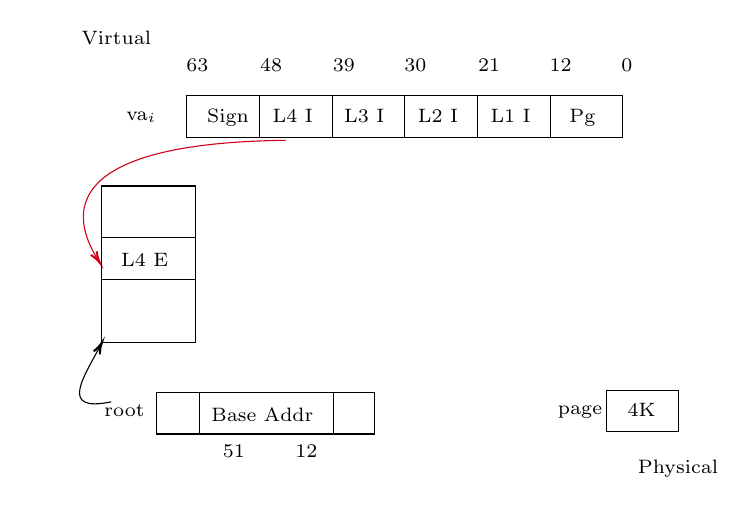
\begin{tikzpicture}[x=0.75pt,y=0.75pt,yscale=-0.5,xscale=0.5]
%uncomment if require: \path (0,475); %set diagram left start at 0, and has height of 475

%Shape: Rectangle [id:dp8869479989297875] 
\draw   (41,174) -- (131,174) -- (131,325) -- (41,325) -- cycle ;
%Shape: Rectangle [id:dp7099724667488323] 
\draw   (123,87) -- (193,87) -- (193,127) -- (123,127) -- cycle ;
%Shape: Rectangle [id:dp8508583959217406] 
\draw   (193,87) -- (263,87) -- (263,127) -- (193,127) -- cycle ;
%Shape: Rectangle [id:dp6986496293895921] 
\draw   (263,87) -- (333,87) -- (333,127) -- (263,127) -- cycle ;
%Shape: Rectangle [id:dp2230750704478599] 
\draw   (333,87) -- (403,87) -- (403,127) -- (333,127) -- cycle ;
%Shape: Rectangle [id:dp07544178914693411] 
\draw   (403,87) -- (473,87) -- (473,127) -- (403,127) -- cycle ;
%Shape: Rectangle [id:dp7298148351808718] 
\draw   (473,87) -- (543,87) -- (543,127) -- (473,127) -- cycle ;
%Curve Lines [id:da17206639309345872] 
\draw [color={rgb, 255:red, 208; green, 2; blue, 27 }  ,draw opacity=1 ]   (218,130) .. controls (-29.94,132.94) and (23.69,223.28) .. (38.17,246.65) ;
\draw [shift={(39,248)}, rotate = 238.24] [color={rgb, 255:red, 208; green, 2; blue, 27 }  ,draw opacity=1 ][line width=0.75]    (10.93,-3.29) .. controls (6.95,-1.4) and (3.31,-0.3) .. (0,0) .. controls (3.31,0.3) and (6.95,1.4) .. (10.93,3.29)   ;
%Shape: Rectangle [id:dp04086108350789486] 
\draw   (41,224) -- (131,224) -- (131,264) -- (41,264) -- cycle ;
%Curve Lines [id:da11224129552033069] 
\draw    (50,382) .. controls (-2.21,392.84) and (25.15,356.13) .. (40.32,326.36) ;
\draw [shift={(41,325)}, rotate = 116.57] [color={rgb, 255:red, 0; green, 0; blue, 0 }  ][line width=0.75]    (10.93,-3.29) .. controls (6.95,-1.4) and (3.31,-0.3) .. (0,0) .. controls (3.31,0.3) and (6.95,1.4) .. (10.93,3.29)   ;
%Shape: Rectangle [id:dp8245870248668032] 
\draw   (527,371) -- (597,371) -- (597,411) -- (527,411) -- cycle ;
%Shape: Rectangle [id:dp28291416382045] 
\draw   (94,373) -- (135.5,373) -- (135.5,413) -- (94,413) -- cycle ;
%Shape: Rectangle [id:dp8964416375534794] 
\draw   (135.5,373) -- (264.5,373) -- (264.5,413) -- (135.5,413) -- cycle ;
%Shape: Rectangle [id:dp1721650962780874] 
\draw   (264.5,373) -- (304,373) -- (304,413) -- (264.5,413) -- cycle ;

% Text Node
\draw (19,22) node [anchor=north west][inner sep=0.75pt]   [align=left] {{\scriptsize Virtual}};
% Text Node
\draw (555,436) node [anchor=north west][inner sep=0.75pt]   [align=left] {{\scriptsize Physical}};
% Text Node
\draw (140,98) node [anchor=north west][inner sep=0.75pt]   [align=left] {{\scriptsize Sign}};
% Text Node
\draw (203,98) node [anchor=north west][inner sep=0.75pt]   [align=left] {{\scriptsize L4 I}};
% Text Node
\draw (272,98) node [anchor=north west][inner sep=0.75pt]   [align=left] {{\scriptsize L3 I}};
% Text Node
\draw (343,98) node [anchor=north west][inner sep=0.75pt]   [align=left] {{\scriptsize L2 I}};
% Text Node
\draw (413,98) node [anchor=north west][inner sep=0.75pt]   [align=left] {{\scriptsize L1 I}};
% Text Node
\draw (489,98) node [anchor=north west][inner sep=0.75pt]   [align=left] {{\scriptsize Pg}};
% Text Node
\draw (62,100) node [anchor=north west][inner sep=0.75pt]   [align=left] {{\scriptsize va$_i$}};
% Text Node
\draw (41,382) node [anchor=north west][inner sep=0.75pt]   [align=left] {{\scriptsize root}};
% Text Node
\draw (57,236) node [anchor=north west][inner sep=0.75pt]   [align=left] {{\scriptsize L4 E}};
% Text Node
\draw (478,384) node [anchor=north west][inner sep=0.75pt]   [align=left] {{\scriptsize page}};
% Text Node
\draw (545,381) node [anchor=north west][inner sep=0.75pt]   [align=left] {{\scriptsize 4K}};
% Text Node
\draw (155,421) node [anchor=north west][inner sep=0.75pt]   [align=left] {{\scriptsize 51}};
% Text Node
\draw (225,421) node [anchor=north west][inner sep=0.75pt]   [align=left] {{\scriptsize 12}};
% Text Node
\draw (144,385) node [anchor=north west][inner sep=0.75pt]   [align=left] {{\scriptsize Base Addr}};
% Text Node
\draw (120,49) node [anchor=north west][inner sep=0.75pt]   [align=left] {{\scriptsize 63}};
% Text Node
\draw (191,49) node [anchor=north west][inner sep=0.75pt]   [align=left] {{\scriptsize 48}};
% Text Node
\draw (261,49) node [anchor=north west][inner sep=0.75pt]   [align=left] {{\scriptsize 39}};
% Text Node
\draw (330,49) node [anchor=north west][inner sep=0.75pt]   [align=left] {{\scriptsize 30}};
% Text Node
\draw (401,49) node [anchor=north west][inner sep=0.75pt]   [align=left] {{\scriptsize 21}};
% Text Node
\draw (470,49) node [anchor=north west][inner sep=0.75pt]   [align=left] {{\scriptsize 12}};
% Text Node
\draw (539,49) node [anchor=north west][inner sep=0.75pt]   [align=left] {{\scriptsize 0}};


\end{tikzpicture}
        \caption{A New L4 Entry}
        \label{fig:enter-label}
    \end{figure}
    \column{.4\textwidth}
\begin{lstlisting}[style=CStyleNum, basicstyle=\tiny]
static pte_t *pte_nxt_table (pte_t *entry){
 pte_t *next;
 // If not already present, try to allocate
 if (!entry->present){
  if (!pte_alloc(&next)) {
   return NULL;
  }
  entry->pfn = PTE_PFN((uintptr_t) next);
  entry->present = 1;
  } else {
   uintptr_t next_phys_addr = PTE_PFN_TO_ADDR(entry->pfn);        
   uintptr_t next_virt_addr = (uintptr_t) P2V(next_phys_addr);
   next = (pte_t *) next_virt_addr;
  }
  return next;
}   
pte_t *walkpgdir(pte_t *l4, void *va){ 
 pte_t *l4_entry = &l4[L4I(va)];
\end{lstlisting}
\end{columns}
\end{frame}
%5-----------------------------------------------------
\begin{frame}[fragile]{Sharing Physical Page Tables}
\begin{columns}[c]
\column{.59\textwidth}    
    \begin{figure}
        \centering
\tikzset{every picture/.style={line width=0.75pt}} %set default line width to 0.75pt        

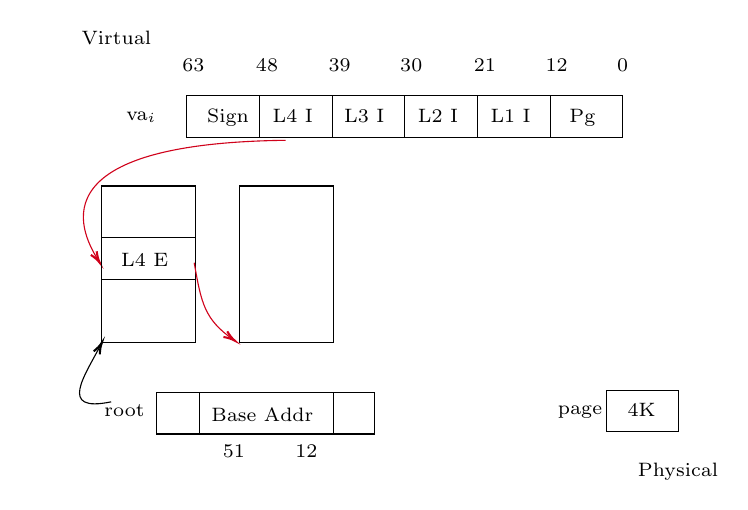
\begin{tikzpicture}[x=0.75pt,y=0.75pt,yscale=-0.5,xscale=0.5]
%uncomment if require: \path (0,475); %set diagram left start at 0, and has height of 475

%Shape: Rectangle [id:dp45793901803276027] 
\draw   (41,174) -- (131,174) -- (131,325) -- (41,325) -- cycle ;
%Shape: Rectangle [id:dp24945660577207507] 
\draw   (174,174) -- (264,174) -- (264,325) -- (174,325) -- cycle ;
%Shape: Rectangle [id:dp2849248657438319] 
\draw   (123,87) -- (193,87) -- (193,127) -- (123,127) -- cycle ;
%Shape: Rectangle [id:dp4457469010684947] 
\draw   (193,87) -- (263,87) -- (263,127) -- (193,127) -- cycle ;
%Shape: Rectangle [id:dp03967656975974165] 
\draw   (263,87) -- (333,87) -- (333,127) -- (263,127) -- cycle ;
%Shape: Rectangle [id:dp14908759208424827] 
\draw   (333,87) -- (403,87) -- (403,127) -- (333,127) -- cycle ;
%Shape: Rectangle [id:dp6432796161085133] 
\draw   (403,87) -- (473,87) -- (473,127) -- (403,127) -- cycle ;
%Shape: Rectangle [id:dp058514064406877564] 
\draw   (473,87) -- (543,87) -- (543,127) -- (473,127) -- cycle ;
%Curve Lines [id:da450406414039652] 
\draw [color={rgb, 255:red, 208; green, 2; blue, 27 }  ,draw opacity=1 ]   (218,130) .. controls (-29.94,132.94) and (23.69,223.28) .. (38.17,246.65) ;
\draw [shift={(39,248)}, rotate = 238.24] [color={rgb, 255:red, 208; green, 2; blue, 27 }  ,draw opacity=1 ][line width=0.75]    (10.93,-3.29) .. controls (6.95,-1.4) and (3.31,-0.3) .. (0,0) .. controls (3.31,0.3) and (6.95,1.4) .. (10.93,3.29)   ;
%Shape: Rectangle [id:dp029111323305148984] 
\draw   (41,224) -- (131,224) -- (131,264) -- (41,264) -- cycle ;
%Curve Lines [id:da1030994483303791] 
\draw    (50,382) .. controls (-2.21,392.84) and (25.15,356.13) .. (40.32,326.36) ;
\draw [shift={(41,325)}, rotate = 116.57] [color={rgb, 255:red, 0; green, 0; blue, 0 }  ][line width=0.75]    (10.93,-3.29) .. controls (6.95,-1.4) and (3.31,-0.3) .. (0,0) .. controls (3.31,0.3) and (6.95,1.4) .. (10.93,3.29)   ;
%Curve Lines [id:da7969408682002264] 
\draw [color={rgb, 255:red, 208; green, 2; blue, 27 }  ,draw opacity=1 ]   (130,248) .. controls (136.9,287.4) and (139.91,302.54) .. (167.71,322.1) ;
\draw [shift={(169,323)}, rotate = 214.59] [color={rgb, 255:red, 208; green, 2; blue, 27 }  ,draw opacity=1 ][line width=0.75]    (10.93,-3.29) .. controls (6.95,-1.4) and (3.31,-0.3) .. (0,0) .. controls (3.31,0.3) and (6.95,1.4) .. (10.93,3.29)   ;
%Shape: Rectangle [id:dp5497266477220895] 
\draw   (527,371) -- (597,371) -- (597,411) -- (527,411) -- cycle ;
%Shape: Rectangle [id:dp6279506536662616] 
\draw   (94,373) -- (135.5,373) -- (135.5,413) -- (94,413) -- cycle ;
%Shape: Rectangle [id:dp9431298808401525] 
\draw   (135.5,373) -- (264.5,373) -- (264.5,413) -- (135.5,413) -- cycle ;
%Shape: Rectangle [id:dp908327665750533] 
\draw   (264.5,373) -- (304,373) -- (304,413) -- (264.5,413) -- cycle ;

% Text Node
\draw (19,22) node [anchor=north west][inner sep=0.75pt]   [align=left] {{\scriptsize Virtual}};
% Text Node
\draw (555,438) node [anchor=north west][inner sep=0.75pt]   [align=left] {{\scriptsize Physical}};
% Text Node
\draw (140,98) node [anchor=north west][inner sep=0.75pt]   [align=left] {{\scriptsize Sign}};
% Text Node
\draw (203,98) node [anchor=north west][inner sep=0.75pt]   [align=left] {{\scriptsize L4 I}};
% Text Node
\draw (272,98) node [anchor=north west][inner sep=0.75pt]   [align=left] {{\scriptsize L3 I}};
% Text Node
\draw (343,98) node [anchor=north west][inner sep=0.75pt]   [align=left] {{\scriptsize L2 I}};
% Text Node
\draw (413,98) node [anchor=north west][inner sep=0.75pt]   [align=left] {{\scriptsize L1 I}};
% Text Node
\draw (489,98) node [anchor=north west][inner sep=0.75pt]   [align=left] {{\scriptsize Pg}};
% Text Node
\draw (62,100) node [anchor=north west][inner sep=0.75pt]   [align=left] {{\scriptsize va$_i$}};
% Text Node
\draw (41,382) node [anchor=north west][inner sep=0.75pt]   [align=left] {{\scriptsize root}};
% Text Node
\draw (57,236) node [anchor=north west][inner sep=0.75pt]   [align=left] {{\scriptsize L4 E}};
% Text Node
\draw (478,384) node [anchor=north west][inner sep=0.75pt]   [align=left] {{\scriptsize page}};
% Text Node
\draw (545,381) node [anchor=north west][inner sep=0.75pt]   [align=left] {{\scriptsize 4K}};
% Text Node
\draw (155,421) node [anchor=north west][inner sep=0.75pt]   [align=left] {{\scriptsize 51}};
% Text Node
\draw (225,421) node [anchor=north west][inner sep=0.75pt]   [align=left] {{\scriptsize 12}};
% Text Node
\draw (144,385) node [anchor=north west][inner sep=0.75pt]   [align=left] {{\scriptsize Base Addr}};
% Text Node
\draw (116,49) node [anchor=north west][inner sep=0.75pt]   [align=left] {{\scriptsize 63}};
% Text Node
\draw (187,49) node [anchor=north west][inner sep=0.75pt]   [align=left] {{\scriptsize 48}};
% Text Node
\draw (257,49) node [anchor=north west][inner sep=0.75pt]   [align=left] {{\scriptsize 39}};
% Text Node
\draw (326,49) node [anchor=north west][inner sep=0.75pt]   [align=left] {{\scriptsize 30}};
% Text Node
\draw (397,49) node [anchor=north west][inner sep=0.75pt]   [align=left] {{\scriptsize 21}};
% Text Node
\draw (466,49) node [anchor=north west][inner sep=0.75pt]   [align=left] {{\scriptsize 12}};
% Text Node
\draw (535,49) node [anchor=north west][inner sep=0.75pt]   [align=left] {{\scriptsize 0}};


\end{tikzpicture}
        \caption{Accessing to Table L3}
        \label{fig:enter-label}
    \end{figure}
    \column{.4\textwidth}
\begin{lstlisting}[style=CStyleNum, basicstyle=\tiny]
static pte_t *pte_nxt_table (pte_t *entry){
 pte_t *next;
 // If not already present, try to allocate
 if (!entry->present){
  if (!pte_alloc(&next)) {
   return NULL;
  }
  entry->pfn = PTE_PFN((uintptr_t) next);
  entry->present = 1;
  } else {
   uintptr_t next_phys_addr = PTE_PFN_TO_ADDR(entry->pfn);        
   uintptr_t next_virt_addr = (uintptr_t) P2V(next_phys_addr);
   next = (pte_t *) next_virt_addr;
  }
  return next;
}   
pte_t *walkpgdir(pte_t *l4, void *va){ 
 pte_t *l4_entry = &l4[L4I(va)];
 pte_t *l3 = pte_nxt_table(l4_entry);
}

\end{lstlisting}
\end{columns}
\end{frame}
%6------------------------------------------------------
\begin{frame}[fragile]{Sharing Physical Page Tables}
\begin{columns}[c]
\column{.59\textwidth}    
    \begin{figure}
        \centering



\tikzset{every picture/.style={line width=0.75pt}} %set default line width to 0.75pt        

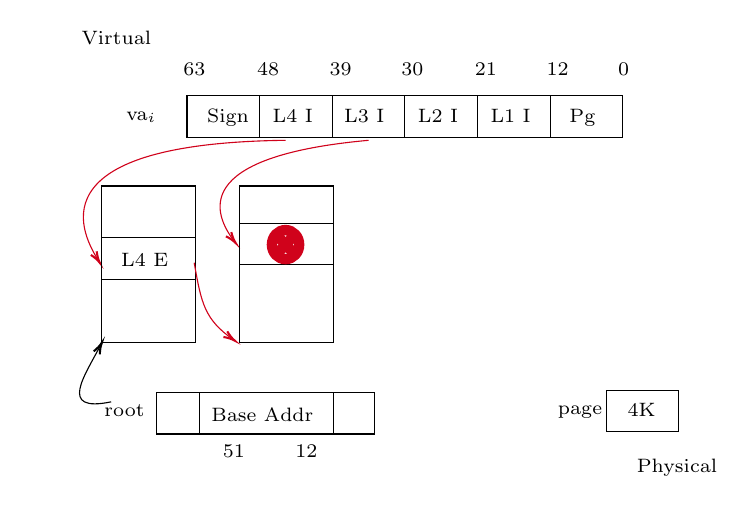
\begin{tikzpicture}[x=0.75pt,y=0.75pt,yscale=-0.5,xscale=0.5]
%uncomment if require: \path (0,467); %set diagram left start at 0, and has height of 467

%Shape: Rectangle [id:dp7491808624328888] 
\draw   (42,170) -- (132,170) -- (132,321) -- (42,321) -- cycle ;
%Shape: Rectangle [id:dp6643737399547691] 
\draw   (175,170) -- (265,170) -- (265,321) -- (175,321) -- cycle ;
%Shape: Rectangle [id:dp012971411714079562] 
\draw   (124,83) -- (194,83) -- (194,123) -- (124,123) -- cycle ;
%Shape: Rectangle [id:dp9764389175430748] 
\draw   (194,83) -- (264,83) -- (264,123) -- (194,123) -- cycle ;
%Shape: Rectangle [id:dp5344228085203682] 
\draw   (264,83) -- (334,83) -- (334,123) -- (264,123) -- cycle ;
%Shape: Rectangle [id:dp8525629842072366] 
\draw   (334,83) -- (404,83) -- (404,123) -- (334,123) -- cycle ;
%Shape: Rectangle [id:dp003949681086953483] 
\draw   (404,83) -- (474,83) -- (474,123) -- (404,123) -- cycle ;
%Shape: Rectangle [id:dp6045496768799752] 
\draw   (474,83) -- (544,83) -- (544,123) -- (474,123) -- cycle ;
%Curve Lines [id:da22346492249504468] 
\draw [color={rgb, 255:red, 208; green, 2; blue, 27 }  ,draw opacity=1 ]   (219,126) .. controls (-28.94,128.94) and (24.69,219.28) .. (39.17,242.65) ;
\draw [shift={(40,244)}, rotate = 238.24] [color={rgb, 255:red, 208; green, 2; blue, 27 }  ,draw opacity=1 ][line width=0.75]    (10.93,-3.29) .. controls (6.95,-1.4) and (3.31,-0.3) .. (0,0) .. controls (3.31,0.3) and (6.95,1.4) .. (10.93,3.29)   ;
%Shape: Rectangle [id:dp0864061964273144] 
\draw   (42,220) -- (132,220) -- (132,260) -- (42,260) -- cycle ;
%Curve Lines [id:da6693242212978325] 
\draw [color={rgb, 255:red, 208; green, 2; blue, 27 }  ,draw opacity=1 ]   (299,126) .. controls (125.54,141.68) and (149.92,197.7) .. (169.79,223.46) ;
\draw [shift={(171,225)}, rotate = 231.34] [color={rgb, 255:red, 208; green, 2; blue, 27 }  ,draw opacity=1 ][line width=0.75]    (10.93,-3.29) .. controls (6.95,-1.4) and (3.31,-0.3) .. (0,0) .. controls (3.31,0.3) and (6.95,1.4) .. (10.93,3.29)   ;
%Shape: Rectangle [id:dp18824071319016822] 
\draw   (175,206) -- (265,206) -- (265,246) -- (175,246) -- cycle ;
%Curve Lines [id:da11429721404151838] 
\draw    (51,378) .. controls (-1.21,388.84) and (26.15,352.13) .. (41.32,322.36) ;
\draw [shift={(42,321)}, rotate = 116.57] [color={rgb, 255:red, 0; green, 0; blue, 0 }  ][line width=0.75]    (10.93,-3.29) .. controls (6.95,-1.4) and (3.31,-0.3) .. (0,0) .. controls (3.31,0.3) and (6.95,1.4) .. (10.93,3.29)   ;
%Curve Lines [id:da6229058140975907] 
\draw [color={rgb, 255:red, 208; green, 2; blue, 27 }  ,draw opacity=1 ]   (131,244) .. controls (137.9,283.4) and (140.91,298.54) .. (168.71,318.1) ;
\draw [shift={(170,319)}, rotate = 214.59] [color={rgb, 255:red, 208; green, 2; blue, 27 }  ,draw opacity=1 ][line width=0.75]    (10.93,-3.29) .. controls (6.95,-1.4) and (3.31,-0.3) .. (0,0) .. controls (3.31,0.3) and (6.95,1.4) .. (10.93,3.29)   ;
%Shape: Rectangle [id:dp2289900447558617] 
\draw   (528,367) -- (598,367) -- (598,407) -- (528,407) -- cycle ;
%Shape: Rectangle [id:dp7118085715057048] 
\draw   (95,369) -- (136.5,369) -- (136.5,409) -- (95,409) -- cycle ;
%Shape: Rectangle [id:dp029487555457707648] 
\draw   (136.5,369) -- (265.5,369) -- (265.5,409) -- (136.5,409) -- cycle ;
%Shape: Rectangle [id:dp621249101472356] 
\draw   (265.5,369) -- (305,369) -- (305,409) -- (265.5,409) -- cycle ;
%Shape: Light Bulb [id:dp5269580683708] 
\draw  [color={rgb, 255:red, 208; green, 2; blue, 27 }  ,draw opacity=1 ][line width=3.75]  (205.88,226.5) .. controls (205.88,218.77) and (211.75,212.5) .. (219,212.5) .. controls (226.25,212.5) and (232.13,218.77) .. (232.13,226.5) .. controls (232.13,234.23) and (226.25,240.5) .. (219,240.5) .. controls (211.75,240.5) and (205.88,234.23) .. (205.88,226.5) -- cycle (209.66,216.53) -- (228.35,236.47) (228.35,216.53) -- (209.66,236.47) (203.25,226.5) -- (205.88,226.5) (232.13,226.5) -- (234.75,226.5) ;

% Text Node
\draw (20,18) node [anchor=north west][inner sep=0.75pt]   [align=left] {{\scriptsize Virtual}};
% Text Node
\draw (555,431) node [anchor=north west][inner sep=0.75pt]   [align=left] {{\scriptsize Physical}};
% Text Node
\draw (141,94) node [anchor=north west][inner sep=0.75pt]   [align=left] {{\scriptsize Sign}};
% Text Node
\draw (204,94) node [anchor=north west][inner sep=0.75pt]   [align=left] {{\scriptsize L4 I}};
% Text Node
\draw (273,94) node [anchor=north west][inner sep=0.75pt]   [align=left] {{\scriptsize L3 I}};
% Text Node
\draw (344,94) node [anchor=north west][inner sep=0.75pt]   [align=left] {{\scriptsize L2 I}};
% Text Node
\draw (414,94) node [anchor=north west][inner sep=0.75pt]   [align=left] {{\scriptsize L1 I}};
% Text Node
\draw (490,94) node [anchor=north west][inner sep=0.75pt]   [align=left] {{\scriptsize Pg}};
% Text Node
\draw (63,96) node [anchor=north west][inner sep=0.75pt]   [align=left] {{\scriptsize va$_i$}};
% Text Node
\draw (42,378) node [anchor=north west][inner sep=0.75pt]   [align=left] {{\scriptsize root}};
% Text Node
\draw (58,232) node [anchor=north west][inner sep=0.75pt]   [align=left] {{\scriptsize L4 E}};
% Text Node
\draw (479,380) node [anchor=north west][inner sep=0.75pt]   [align=left] {{\scriptsize page}};
% Text Node
\draw (546,377) node [anchor=north west][inner sep=0.75pt]   [align=left] {{\scriptsize 4K}};
% Text Node
\draw (156,417) node [anchor=north west][inner sep=0.75pt]   [align=left] {{\scriptsize 51}};
% Text Node
\draw (226,417) node [anchor=north west][inner sep=0.75pt]   [align=left] {{\scriptsize 12}};
% Text Node
\draw (145,381) node [anchor=north west][inner sep=0.75pt]   [align=left] {{\scriptsize Base Addr}};
% Text Node
\draw (118,49) node [anchor=north west][inner sep=0.75pt]   [align=left] {{\scriptsize 63}};
% Text Node
\draw (189,49) node [anchor=north west][inner sep=0.75pt]   [align=left] {{\scriptsize 48}};
% Text Node
\draw (259,49) node [anchor=north west][inner sep=0.75pt]   [align=left] {{\scriptsize 39}};
% Text Node
\draw (328,49) node [anchor=north west][inner sep=0.75pt]   [align=left] {{\scriptsize 30}};
% Text Node
\draw (399,49) node [anchor=north west][inner sep=0.75pt]   [align=left] {{\scriptsize 21}};
% Text Node
\draw (468,49) node [anchor=north west][inner sep=0.75pt]   [align=left] {{\scriptsize 12}};
% Text Node
\draw (537,49) node [anchor=north west][inner sep=0.75pt]   [align=left] {{\scriptsize 0}};


\end{tikzpicture}
        \caption{Missing L3 Entry}
        \label{fig:enter-label}
    \end{figure}
    \column{.4\textwidth}
\begin{lstlisting}[style=CStyleNum, basicstyle=\tiny]
static pte_t *pte_nxt_table (pte_t *entry){
 pte_t *next;
 // If not already present, try to allocate
 if (!entry->present){
  if (!pte_alloc(&next)) {
   return NULL;
  }
  entry->pfn = PTE_PFN((uintptr_t) next);
  entry->present = 1;
  } else {
   uintptr_t next_phys_addr = PTE_PFN_TO_ADDR(entry->pfn);        
   uintptr_t next_virt_addr = (uintptr_t) P2V(next_phys_addr);
   next = (pte_t *) next_virt_addr;
  }
  return next;
}   
pte_t *walkpgdir(pte_t *l4, void *va){ 
 pte_t *l4_entry = &l4[L4I(va)];
 pte_t *l3 = pte_nxt_table(l4_entry);
}

\end{lstlisting}
\end{columns}
\end{frame}
%7-------------------------------------------------------
\begin{frame}[fragile]{Sharing Physical Page Tables}
\begin{columns}[c]
\column{.59\textwidth}    
    \begin{figure}
        \centering

\tikzset{every picture/.style={line width=0.75pt}} %set default line width to 0.75pt        

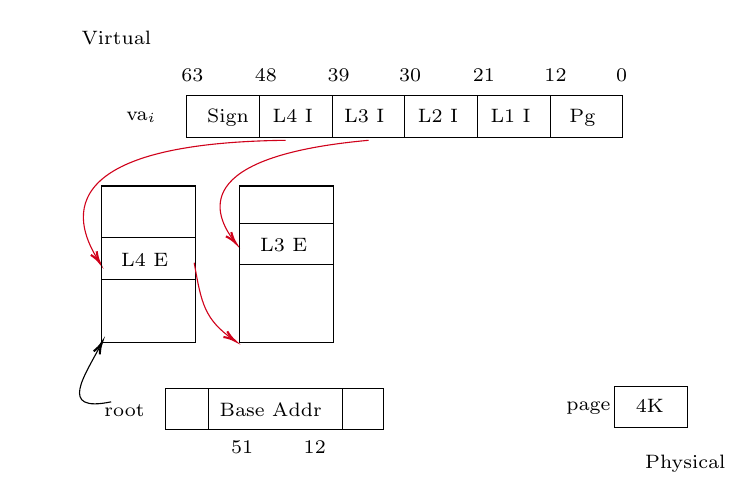
\begin{tikzpicture}[x=0.75pt,y=0.75pt,yscale=-0.5,xscale=0.5]
%uncomment if require: \path (0,456); %set diagram left start at 0, and has height of 456

%Shape: Rectangle [id:dp11825905074984977] 
\draw   (45,164) -- (135,164) -- (135,315) -- (45,315) -- cycle ;
%Shape: Rectangle [id:dp539699855643808] 
\draw   (178,164) -- (268,164) -- (268,315) -- (178,315) -- cycle ;
%Shape: Rectangle [id:dp15623456467051944] 
\draw   (127,77) -- (197,77) -- (197,117) -- (127,117) -- cycle ;
%Shape: Rectangle [id:dp10498357757801946] 
\draw   (197,77) -- (267,77) -- (267,117) -- (197,117) -- cycle ;
%Shape: Rectangle [id:dp2707689368686157] 
\draw   (267,77) -- (337,77) -- (337,117) -- (267,117) -- cycle ;
%Shape: Rectangle [id:dp047644415643700366] 
\draw   (337,77) -- (407,77) -- (407,117) -- (337,117) -- cycle ;
%Shape: Rectangle [id:dp12929158307466215] 
\draw   (407,77) -- (477,77) -- (477,117) -- (407,117) -- cycle ;
%Shape: Rectangle [id:dp819840906555648] 
\draw   (477,77) -- (547,77) -- (547,117) -- (477,117) -- cycle ;
%Curve Lines [id:da5514743914050342] 
\draw [color={rgb, 255:red, 208; green, 2; blue, 27 }  ,draw opacity=1 ]   (222,120) .. controls (-25.94,122.94) and (27.69,213.28) .. (42.17,236.65) ;
\draw [shift={(43,238)}, rotate = 238.24] [color={rgb, 255:red, 208; green, 2; blue, 27 }  ,draw opacity=1 ][line width=0.75]    (10.93,-3.29) .. controls (6.95,-1.4) and (3.31,-0.3) .. (0,0) .. controls (3.31,0.3) and (6.95,1.4) .. (10.93,3.29)   ;
%Shape: Rectangle [id:dp6238026337192846] 
\draw   (45,214) -- (135,214) -- (135,254) -- (45,254) -- cycle ;
%Curve Lines [id:da3305133907131548] 
\draw [color={rgb, 255:red, 208; green, 2; blue, 27 }  ,draw opacity=1 ]   (302,120) .. controls (128.54,135.68) and (152.92,191.7) .. (172.79,217.46) ;
\draw [shift={(174,219)}, rotate = 231.34] [color={rgb, 255:red, 208; green, 2; blue, 27 }  ,draw opacity=1 ][line width=0.75]    (10.93,-3.29) .. controls (6.95,-1.4) and (3.31,-0.3) .. (0,0) .. controls (3.31,0.3) and (6.95,1.4) .. (10.93,3.29)   ;
%Shape: Rectangle [id:dp899160406090266] 
\draw   (178,200) -- (268,200) -- (268,240) -- (178,240) -- cycle ;
%Curve Lines [id:da5153902998483901] 
\draw    (54,372) .. controls (1.79,382.84) and (29.15,346.13) .. (44.32,316.36) ;
\draw [shift={(45,315)}, rotate = 116.57] [color={rgb, 255:red, 0; green, 0; blue, 0 }  ][line width=0.75]    (10.93,-3.29) .. controls (6.95,-1.4) and (3.31,-0.3) .. (0,0) .. controls (3.31,0.3) and (6.95,1.4) .. (10.93,3.29)   ;
%Curve Lines [id:da5347752483663382] 
\draw [color={rgb, 255:red, 208; green, 2; blue, 27 }  ,draw opacity=1 ]   (134,238) .. controls (140.9,277.4) and (143.91,292.54) .. (171.71,312.1) ;
\draw [shift={(173,313)}, rotate = 214.59] [color={rgb, 255:red, 208; green, 2; blue, 27 }  ,draw opacity=1 ][line width=0.75]    (10.93,-3.29) .. controls (6.95,-1.4) and (3.31,-0.3) .. (0,0) .. controls (3.31,0.3) and (6.95,1.4) .. (10.93,3.29)   ;
%Shape: Rectangle [id:dp5990812045987151] 
\draw   (539,357) -- (609,357) -- (609,397) -- (539,397) -- cycle ;
%Shape: Rectangle [id:dp15447291578285371] 
\draw   (106,359) -- (147.5,359) -- (147.5,399) -- (106,399) -- cycle ;
%Shape: Rectangle [id:dp18590945808949733] 
\draw   (147.5,359) -- (276.5,359) -- (276.5,399) -- (147.5,399) -- cycle ;
%Shape: Rectangle [id:dp3281524610311157] 
\draw   (276.5,359) -- (316,359) -- (316,399) -- (276.5,399) -- cycle ;

% Text Node
\draw (23,12) node [anchor=north west][inner sep=0.75pt]   [align=left] {{\scriptsize Virtual}};
% Text Node
\draw (144,88) node [anchor=north west][inner sep=0.75pt]   [align=left] {{\scriptsize Sign}};
% Text Node
\draw (207,88) node [anchor=north west][inner sep=0.75pt]   [align=left] {{\scriptsize L4 I}};
% Text Node
\draw (276,88) node [anchor=north west][inner sep=0.75pt]   [align=left] {{\scriptsize L3 I}};
% Text Node
\draw (347,88) node [anchor=north west][inner sep=0.75pt]   [align=left] {{\scriptsize L2 I}};
% Text Node
\draw (417,88) node [anchor=north west][inner sep=0.75pt]   [align=left] {{\scriptsize L1 I}};
% Text Node
\draw (493,88) node [anchor=north west][inner sep=0.75pt]   [align=left] {{\scriptsize Pg}};
% Text Node
\draw (66,90) node [anchor=north west][inner sep=0.75pt]   [align=left] {{\scriptsize va$_i$}};
% Text Node
\draw (45,372) node [anchor=north west][inner sep=0.75pt]   [align=left] {{\scriptsize root}};
% Text Node
\draw (61,226) node [anchor=north west][inner sep=0.75pt]   [align=left] {{\scriptsize L4 E}};
% Text Node
\draw (195,212) node [anchor=north west][inner sep=0.75pt]   [align=left] {{\scriptsize L3 E}};
% Text Node
\draw (119,49) node [anchor=north west][inner sep=0.75pt]   [align=left] {{\scriptsize 63}};
% Text Node
\draw (190,49) node [anchor=north west][inner sep=0.75pt]   [align=left] {{\scriptsize 48}};
% Text Node
\draw (260,49) node [anchor=north west][inner sep=0.75pt]   [align=left] {{\scriptsize 39}};
% Text Node
\draw (329,49) node [anchor=north west][inner sep=0.75pt]   [align=left] {{\scriptsize 30}};
% Text Node
\draw (400,49) node [anchor=north west][inner sep=0.75pt]   [align=left] {{\scriptsize 21}};
% Text Node
\draw (469,49) node [anchor=north west][inner sep=0.75pt]   [align=left] {{\scriptsize 12}};
% Text Node
\draw (538,49) node [anchor=north west][inner sep=0.75pt]   [align=left] {{\scriptsize 0}};
% Text Node
\draw (566,421) node [anchor=north west][inner sep=0.75pt]   [align=left] {{\scriptsize Physical}};
% Text Node
\draw (490,370) node [anchor=north west][inner sep=0.75pt]   [align=left] {{\scriptsize page}};
% Text Node
\draw (557,367) node [anchor=north west][inner sep=0.75pt]   [align=left] {{\scriptsize 4K}};
% Text Node
\draw (167,407) node [anchor=north west][inner sep=0.75pt]   [align=left] {{\scriptsize 51}};
% Text Node
\draw (237,407) node [anchor=north west][inner sep=0.75pt]   [align=left] {{\scriptsize 12}};
% Text Node
\draw (156,371) node [anchor=north west][inner sep=0.75pt]   [align=left] {{\scriptsize Base Addr}};


\end{tikzpicture}
        \caption{A New L3 Entry}
        \label{fig:enter-label}
    \end{figure}
    \column{.4\textwidth}
\begin{lstlisting}[style=CStyleNum, basicstyle=\tiny]
static pte_t *pte_nxt_table (pte_t *entry){
 pte_t *next;
 // If not already present, try to allocate
 if (!entry->present){
  if (!pte_alloc(&next)) {
   return NULL;
  }
  entry->pfn = PTE_PFN((uintptr_t) next);
  entry->present = 1;
  } else {
   uintptr_t next_phys_addr = PTE_PFN_TO_ADDR(entry->pfn);        
   uintptr_t next_virt_addr = (uintptr_t) P2V(next_phys_addr);
   next = (pte_t *) next_virt_addr;
  }
  return next;
}   
pte_t *walkpgdir(pte_t *l4, void *va){ 
 pte_t *l4_entry = &l4[L4I(va)];
 pte_t *l3 = pte_nxt_table(l4_entry);
 pte_t *l3_entry = &l3[L3I(va)];
}

\end{lstlisting}
\end{columns}
\end{frame}
%8-------------------------------------------------------
\begin{frame}[fragile]{Sharing Physical Page Tables}
\begin{columns}[c]
\column{.59\textwidth}    
    \begin{figure}
        \centering
\tikzset{every picture/.style={line width=0.75pt}} %set default line width to 0.75pt        
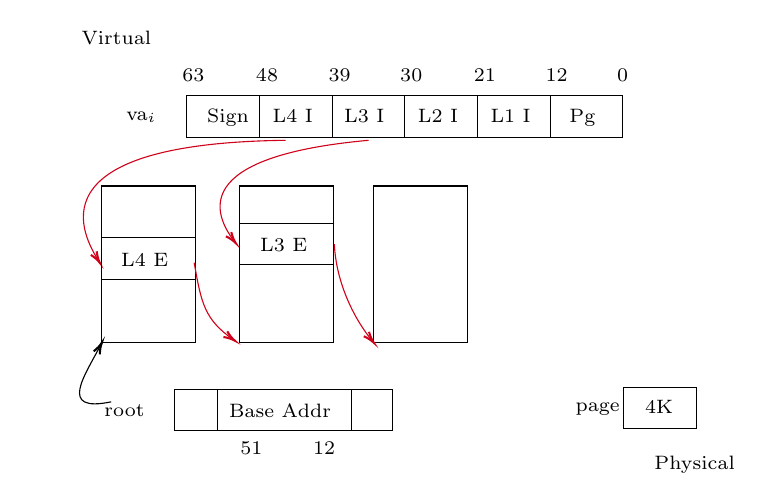
\begin{tikzpicture}[x=0.75pt,y=0.75pt,yscale=-0.5,xscale=0.5]
%uncomment if require: \path (0,456); %set diagram left start at 0, and has height of 456

%Shape: Rectangle [id:dp7310596398285061] 
\draw   (45,164) -- (135,164) -- (135,315) -- (45,315) -- cycle ;
%Shape: Rectangle [id:dp10058608093526056] 
\draw   (178,164) -- (268,164) -- (268,315) -- (178,315) -- cycle ;
%Shape: Rectangle [id:dp9023930159852462] 
\draw   (307,164) -- (397,164) -- (397,315) -- (307,315) -- cycle ;
%Shape: Rectangle [id:dp640312238204892] 
\draw   (127,77) -- (197,77) -- (197,117) -- (127,117) -- cycle ;
%Shape: Rectangle [id:dp1635993034746881] 
\draw   (197,77) -- (267,77) -- (267,117) -- (197,117) -- cycle ;
%Shape: Rectangle [id:dp2897714079082683] 
\draw   (267,77) -- (337,77) -- (337,117) -- (267,117) -- cycle ;
%Shape: Rectangle [id:dp6419399714101042] 
\draw   (337,77) -- (407,77) -- (407,117) -- (337,117) -- cycle ;
%Shape: Rectangle [id:dp07485902184608673] 
\draw   (407,77) -- (477,77) -- (477,117) -- (407,117) -- cycle ;
%Shape: Rectangle [id:dp2364936526671133] 
\draw   (477,77) -- (547,77) -- (547,117) -- (477,117) -- cycle ;
%Curve Lines [id:da27036934093820175] 
\draw [color={rgb, 255:red, 208; green, 2; blue, 27 }  ,draw opacity=1 ]   (222,120) .. controls (-25.94,122.94) and (27.69,213.28) .. (42.17,236.65) ;
\draw [shift={(43,238)}, rotate = 238.24] [color={rgb, 255:red, 208; green, 2; blue, 27 }  ,draw opacity=1 ][line width=0.75]    (10.93,-3.29) .. controls (6.95,-1.4) and (3.31,-0.3) .. (0,0) .. controls (3.31,0.3) and (6.95,1.4) .. (10.93,3.29)   ;
%Shape: Rectangle [id:dp11316077656388579] 
\draw   (45,214) -- (135,214) -- (135,254) -- (45,254) -- cycle ;
%Curve Lines [id:da3923169661433725] 
\draw [color={rgb, 255:red, 208; green, 2; blue, 27 }  ,draw opacity=1 ]   (302,120) .. controls (128.54,135.68) and (152.92,191.7) .. (172.79,217.46) ;
\draw [shift={(174,219)}, rotate = 231.34] [color={rgb, 255:red, 208; green, 2; blue, 27 }  ,draw opacity=1 ][line width=0.75]    (10.93,-3.29) .. controls (6.95,-1.4) and (3.31,-0.3) .. (0,0) .. controls (3.31,0.3) and (6.95,1.4) .. (10.93,3.29)   ;
%Shape: Rectangle [id:dp9729239351714787] 
\draw   (178,200) -- (268,200) -- (268,240) -- (178,240) -- cycle ;
%Curve Lines [id:da7403026153668966] 
\draw    (54,372) .. controls (1.79,382.84) and (29.15,346.13) .. (44.32,316.36) ;
\draw [shift={(45,315)}, rotate = 116.57] [color={rgb, 255:red, 0; green, 0; blue, 0 }  ][line width=0.75]    (10.93,-3.29) .. controls (6.95,-1.4) and (3.31,-0.3) .. (0,0) .. controls (3.31,0.3) and (6.95,1.4) .. (10.93,3.29)   ;
%Curve Lines [id:da43786672578528996] 
\draw [color={rgb, 255:red, 208; green, 2; blue, 27 }  ,draw opacity=1 ]   (134,238) .. controls (140.9,277.4) and (143.91,292.54) .. (171.71,312.1) ;
\draw [shift={(173,313)}, rotate = 214.59] [color={rgb, 255:red, 208; green, 2; blue, 27 }  ,draw opacity=1 ][line width=0.75]    (10.93,-3.29) .. controls (6.95,-1.4) and (3.31,-0.3) .. (0,0) .. controls (3.31,0.3) and (6.95,1.4) .. (10.93,3.29)   ;
%Curve Lines [id:da6910869467374454] 
\draw [color={rgb, 255:red, 208; green, 2; blue, 27 }  ,draw opacity=1 ]   (269,220) .. controls (270.95,259) and (289.06,293.25) .. (305.72,313.47) ;
\draw [shift={(307,315)}, rotate = 229.64] [color={rgb, 255:red, 208; green, 2; blue, 27 }  ,draw opacity=1 ][line width=0.75]    (10.93,-3.29) .. controls (6.95,-1.4) and (3.31,-0.3) .. (0,0) .. controls (3.31,0.3) and (6.95,1.4) .. (10.93,3.29)   ;
%Shape: Rectangle [id:dp9591392046076617] 
\draw   (548,358) -- (618,358) -- (618,398) -- (548,398) -- cycle ;
%Shape: Rectangle [id:dp22254421422877968] 
\draw   (115,360) -- (156.5,360) -- (156.5,400) -- (115,400) -- cycle ;
%Shape: Rectangle [id:dp21106266764917692] 
\draw   (156.5,360) -- (285.5,360) -- (285.5,400) -- (156.5,400) -- cycle ;
%Shape: Rectangle [id:dp4819925378892562] 
\draw   (285.5,360) -- (325,360) -- (325,400) -- (285.5,400) -- cycle ;

% Text Node
\draw (23,12) node [anchor=north west][inner sep=0.75pt]   [align=left] {{\scriptsize Virtual}};
% Text Node
\draw (144,88) node [anchor=north west][inner sep=0.75pt]   [align=left] {{\scriptsize Sign}};
% Text Node
\draw (207,88) node [anchor=north west][inner sep=0.75pt]   [align=left] {{\scriptsize L4 I}};
% Text Node
\draw (276,88) node [anchor=north west][inner sep=0.75pt]   [align=left] {{\scriptsize L3 I}};
% Text Node
\draw (347,88) node [anchor=north west][inner sep=0.75pt]   [align=left] {{\scriptsize L2 I}};
% Text Node
\draw (417,88) node [anchor=north west][inner sep=0.75pt]   [align=left] {{\scriptsize L1 I}};
% Text Node
\draw (493,88) node [anchor=north west][inner sep=0.75pt]   [align=left] {{\scriptsize Pg}};
% Text Node
\draw (66,90) node [anchor=north west][inner sep=0.75pt]   [align=left] {{\scriptsize va$_i$}};
% Text Node
\draw (45,372) node [anchor=north west][inner sep=0.75pt]   [align=left] {{\scriptsize root}};
% Text Node
\draw (61,226) node [anchor=north west][inner sep=0.75pt]   [align=left] {{\scriptsize L4 E}};
% Text Node
\draw (195,212) node [anchor=north west][inner sep=0.75pt]   [align=left] {{\scriptsize L3 E}};
% Text Node
\draw (120,49) node [anchor=north west][inner sep=0.75pt]   [align=left] {{\scriptsize 63}};
% Text Node
\draw (191,49) node [anchor=north west][inner sep=0.75pt]   [align=left] {{\scriptsize 48}};
% Text Node
\draw (261,49) node [anchor=north west][inner sep=0.75pt]   [align=left] {{\scriptsize 39}};
% Text Node
\draw (330,49) node [anchor=north west][inner sep=0.75pt]   [align=left] {{\scriptsize 30}};
% Text Node
\draw (401,49) node [anchor=north west][inner sep=0.75pt]   [align=left] {{\scriptsize 21}};
% Text Node
\draw (470,49) node [anchor=north west][inner sep=0.75pt]   [align=left] {{\scriptsize 12}};
% Text Node
\draw (539,49) node [anchor=north west][inner sep=0.75pt]   [align=left] {{\scriptsize 0}};
% Text Node
\draw (575,422) node [anchor=north west][inner sep=0.75pt]   [align=left] {{\scriptsize Physical}};
% Text Node
\draw (499,371) node [anchor=north west][inner sep=0.75pt]   [align=left] {{\scriptsize page}};
% Text Node
\draw (566,368) node [anchor=north west][inner sep=0.75pt]   [align=left] {{\scriptsize 4K}};
% Text Node
\draw (176,408) node [anchor=north west][inner sep=0.75pt]   [align=left] {{\scriptsize 51}};
% Text Node
\draw (246,408) node [anchor=north west][inner sep=0.75pt]   [align=left] {{\scriptsize 12}};
% Text Node
\draw (165,372) node [anchor=north west][inner sep=0.75pt]   [align=left] {{\scriptsize Base Addr}};


\end{tikzpicture}
        \caption{Accessing to L2 Table}
        \label{fig:enter-label}
    \end{figure}
    \column{.4\textwidth}
\begin{lstlisting}[style=CStyleNum, basicstyle=\tiny]
static pte_t *pte_nxt_table (pte_t *entry){
 pte_t *next;
 // If not already present, try to allocate
 if (!entry->present){
  if (!pte_alloc(&next)) {
   return NULL;
  }
  entry->pfn = PTE_PFN((uintptr_t) next);
  entry->present = 1;
  } else {
   uintptr_t next_phys_addr = PTE_PFN_TO_ADDR(entry->pfn);        
   uintptr_t next_virt_addr = (uintptr_t) P2V(next_phys_addr);
   next = (pte_t *) next_virt_addr;
  }
  return next;
}   
pte_t *walkpgdir(pte_t *l4, void *va){ 
 pte_t *l4_entry = &l4[L4I(va)];
 pte_t *l3 = pte_nxt_table(l4_entry);
 pte_t *l3_entry = &l3[L3I(va)];
 pte_t *l2 = pte_nxt_table(l3_entry);
}

\end{lstlisting}
\end{columns}
\end{frame}
%9-------------------------------------------------------
\begin{frame}[fragile]{Sharing Physical Page Tables}
\begin{columns}[c]
\column{.59\textwidth}    
    \begin{figure}
        \centering
\tikzset{every picture/.style={line width=0.75pt}} %set default line width to 0.75pt        

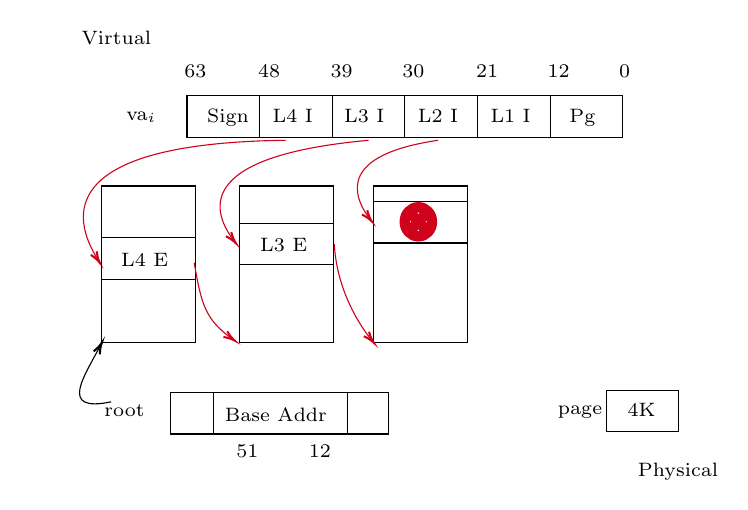
\begin{tikzpicture}[x=0.75pt,y=0.75pt,yscale=-0.5,xscale=0.5]
%uncomment if require: \path (0,466); %set diagram left start at 0, and has height of 466

%Shape: Rectangle [id:dp7225619598463737] 
\draw   (34,168) -- (124,168) -- (124,319) -- (34,319) -- cycle ;
%Shape: Rectangle [id:dp48932315311699215] 
\draw   (167,168) -- (257,168) -- (257,319) -- (167,319) -- cycle ;
%Shape: Rectangle [id:dp6786729581662756] 
\draw   (296,168) -- (386,168) -- (386,319) -- (296,319) -- cycle ;
%Shape: Rectangle [id:dp07115573211590598] 
\draw   (116,81) -- (186,81) -- (186,121) -- (116,121) -- cycle ;
%Shape: Rectangle [id:dp2069239652889001] 
\draw   (186,81) -- (256,81) -- (256,121) -- (186,121) -- cycle ;
%Shape: Rectangle [id:dp09516635470841117] 
\draw   (256,81) -- (326,81) -- (326,121) -- (256,121) -- cycle ;
%Shape: Rectangle [id:dp7459641184318357] 
\draw   (326,81) -- (396,81) -- (396,121) -- (326,121) -- cycle ;
%Shape: Rectangle [id:dp3310050899594881] 
\draw   (396,81) -- (466,81) -- (466,121) -- (396,121) -- cycle ;
%Shape: Rectangle [id:dp5567800275792452] 
\draw   (466,81) -- (536,81) -- (536,121) -- (466,121) -- cycle ;
%Curve Lines [id:da11673018701543181] 
\draw [color={rgb, 255:red, 208; green, 2; blue, 27 }  ,draw opacity=1 ]   (211,124) .. controls (-36.94,126.94) and (16.69,217.28) .. (31.17,240.65) ;
\draw [shift={(32,242)}, rotate = 238.24] [color={rgb, 255:red, 208; green, 2; blue, 27 }  ,draw opacity=1 ][line width=0.75]    (10.93,-3.29) .. controls (6.95,-1.4) and (3.31,-0.3) .. (0,0) .. controls (3.31,0.3) and (6.95,1.4) .. (10.93,3.29)   ;
%Shape: Rectangle [id:dp3602227938188449] 
\draw   (34,218) -- (124,218) -- (124,258) -- (34,258) -- cycle ;
%Curve Lines [id:da1843179981130887] 
\draw [color={rgb, 255:red, 208; green, 2; blue, 27 }  ,draw opacity=1 ]   (291,124) .. controls (117.54,139.68) and (141.92,195.7) .. (161.79,221.46) ;
\draw [shift={(163,223)}, rotate = 231.34] [color={rgb, 255:red, 208; green, 2; blue, 27 }  ,draw opacity=1 ][line width=0.75]    (10.93,-3.29) .. controls (6.95,-1.4) and (3.31,-0.3) .. (0,0) .. controls (3.31,0.3) and (6.95,1.4) .. (10.93,3.29)   ;
%Shape: Rectangle [id:dp3046857411520898] 
\draw   (167,204) -- (257,204) -- (257,244) -- (167,244) -- cycle ;
%Shape: Rectangle [id:dp5559589772091584] 
\draw   (296,183) -- (386,183) -- (386,223) -- (296,223) -- cycle ;
%Curve Lines [id:da7918129198097845] 
\draw [color={rgb, 255:red, 208; green, 2; blue, 27 }  ,draw opacity=1 ]   (358,124) .. controls (263.92,137.72) and (273.56,175.45) .. (292.81,200.48) ;
\draw [shift={(294,202)}, rotate = 231.34] [color={rgb, 255:red, 208; green, 2; blue, 27 }  ,draw opacity=1 ][line width=0.75]    (10.93,-3.29) .. controls (6.95,-1.4) and (3.31,-0.3) .. (0,0) .. controls (3.31,0.3) and (6.95,1.4) .. (10.93,3.29)   ;
%Curve Lines [id:da7916746759816113] 
\draw    (43,376) .. controls (-9.21,386.84) and (18.15,350.13) .. (33.32,320.36) ;
\draw [shift={(34,319)}, rotate = 116.57] [color={rgb, 255:red, 0; green, 0; blue, 0 }  ][line width=0.75]    (10.93,-3.29) .. controls (6.95,-1.4) and (3.31,-0.3) .. (0,0) .. controls (3.31,0.3) and (6.95,1.4) .. (10.93,3.29)   ;
%Curve Lines [id:da4729934938921858] 
\draw [color={rgb, 255:red, 208; green, 2; blue, 27 }  ,draw opacity=1 ]   (123,242) .. controls (129.9,281.4) and (132.91,296.54) .. (160.71,316.1) ;
\draw [shift={(162,317)}, rotate = 214.59] [color={rgb, 255:red, 208; green, 2; blue, 27 }  ,draw opacity=1 ][line width=0.75]    (10.93,-3.29) .. controls (6.95,-1.4) and (3.31,-0.3) .. (0,0) .. controls (3.31,0.3) and (6.95,1.4) .. (10.93,3.29)   ;
%Curve Lines [id:da9453947850126261] 
\draw [color={rgb, 255:red, 208; green, 2; blue, 27 }  ,draw opacity=1 ]   (258,224) .. controls (259.95,263) and (278.06,297.25) .. (294.72,317.47) ;
\draw [shift={(296,319)}, rotate = 229.64] [color={rgb, 255:red, 208; green, 2; blue, 27 }  ,draw opacity=1 ][line width=0.75]    (10.93,-3.29) .. controls (6.95,-1.4) and (3.31,-0.3) .. (0,0) .. controls (3.31,0.3) and (6.95,1.4) .. (10.93,3.29)   ;
%Shape: Rectangle [id:dp6448174490144554] 
\draw   (520,365) -- (590,365) -- (590,405) -- (520,405) -- cycle ;
%Shape: Rectangle [id:dp29238747803903054] 
\draw   (100,367) -- (141.5,367) -- (141.5,407) -- (100,407) -- cycle ;
%Shape: Rectangle [id:dp258550724937215] 
\draw   (141.5,367) -- (270.5,367) -- (270.5,407) -- (141.5,407) -- cycle ;
%Shape: Rectangle [id:dp9613995547256671] 
\draw   (270.5,367) -- (310,367) -- (310,407) -- (270.5,407) -- cycle ;
%Shape: Light Bulb [id:dp4607433802921692] 
\draw  [color={rgb, 255:red, 208; green, 2; blue, 27 }  ,draw opacity=1 ][line width=3.75]  (325.88,202.5) .. controls (325.88,194.77) and (331.75,188.5) .. (339,188.5) .. controls (346.25,188.5) and (352.13,194.77) .. (352.13,202.5) .. controls (352.13,210.23) and (346.25,216.5) .. (339,216.5) .. controls (331.75,216.5) and (325.88,210.23) .. (325.88,202.5) -- cycle (329.66,192.53) -- (348.35,212.47) (348.35,192.53) -- (329.66,212.47) (323.25,202.5) -- (325.88,202.5) (352.13,202.5) -- (354.75,202.5) ;

% Text Node
\draw (12,16) node [anchor=north west][inner sep=0.75pt]   [align=left] {{\scriptsize Virtual}};
% Text Node
\draw (548,432) node [anchor=north west][inner sep=0.75pt]   [align=left] {{\scriptsize Physical}};
% Text Node
\draw (133,92) node [anchor=north west][inner sep=0.75pt]   [align=left] {{\scriptsize Sign}};
% Text Node
\draw (196,92) node [anchor=north west][inner sep=0.75pt]   [align=left] {{\scriptsize L4 I}};
% Text Node
\draw (265,92) node [anchor=north west][inner sep=0.75pt]   [align=left] {{\scriptsize L3 I}};
% Text Node
\draw (336,92) node [anchor=north west][inner sep=0.75pt]   [align=left] {{\scriptsize L2 I}};
% Text Node
\draw (406,92) node [anchor=north west][inner sep=0.75pt]   [align=left] {{\scriptsize L1 I}};
% Text Node
\draw (482,92) node [anchor=north west][inner sep=0.75pt]   [align=left] {{\scriptsize Pg}};
% Text Node
\draw (55,94) node [anchor=north west][inner sep=0.75pt]   [align=left] {{\scriptsize va$_i$}};
% Text Node
\draw (34,376) node [anchor=north west][inner sep=0.75pt]   [align=left] {{\scriptsize root}};
% Text Node
\draw (50,230) node [anchor=north west][inner sep=0.75pt]   [align=left] {{\scriptsize L4 E}};
% Text Node
\draw (184,216) node [anchor=north west][inner sep=0.75pt]   [align=left] {{\scriptsize L3 E}};
% Text Node
\draw (471,378) node [anchor=north west][inner sep=0.75pt]   [align=left] {{\scriptsize page}};
% Text Node
\draw (538,375) node [anchor=north west][inner sep=0.75pt]   [align=left] {{\scriptsize 4K}};
% Text Node
\draw (161,415) node [anchor=north west][inner sep=0.75pt]   [align=left] {{\scriptsize 51}};
% Text Node
\draw (231,415) node [anchor=north west][inner sep=0.75pt]   [align=left] {{\scriptsize 12}};
% Text Node
\draw (150,379) node [anchor=north west][inner sep=0.75pt]   [align=left] {{\scriptsize Base Addr}};
% Text Node
\draw (111,49) node [anchor=north west][inner sep=0.75pt]   [align=left] {{\scriptsize 63}};
% Text Node
\draw (182,49) node [anchor=north west][inner sep=0.75pt]   [align=left] {{\scriptsize 48}};
% Text Node
\draw (252,49) node [anchor=north west][inner sep=0.75pt]   [align=left] {{\scriptsize 39}};
% Text Node
\draw (321,49) node [anchor=north west][inner sep=0.75pt]   [align=left] {{\scriptsize 30}};
% Text Node
\draw (392,49) node [anchor=north west][inner sep=0.75pt]   [align=left] {{\scriptsize 21}};
% Text Node
\draw (461,49) node [anchor=north west][inner sep=0.75pt]   [align=left] {{\scriptsize 12}};
% Text Node
\draw (530,49) node [anchor=north west][inner sep=0.75pt]   [align=left] {{\scriptsize 0}};


\end{tikzpicture}
        \caption{Missing L2 Entry}
        \label{fig:enter-label}
    \end{figure}
    \column{.4\textwidth}
\begin{lstlisting}[style=CStyleNum, basicstyle=\tiny]
static pte_t *pte_nxt_table (pte_t *entry){
 pte_t *next;
 // If not already present, try to allocate
 if (!entry->present){
  if (!pte_alloc(&next)) {
   return NULL;
  }
  entry->pfn = PTE_PFN((uintptr_t) next);
  entry->present = 1;
  } else {
   uintptr_t next_phys_addr = PTE_PFN_TO_ADDR(entry->pfn);        
   uintptr_t next_virt_addr = (uintptr_t) P2V(next_phys_addr);
   next = (pte_t *) next_virt_addr;
  }
  return next;
}   
pte_t *walkpgdir(pte_t *l4, void *va){ 
 pte_t *l4_entry = &l4[L4I(va)];
 pte_t *l3 = pte_nxt_table(l4_entry);
 pte_t *l3_entry = &l3[L3I(va)];
 pte_t *l2 = pte_nxt_table(l3_entry);
}

\end{lstlisting}
\end{columns}
\end{frame}
%10---------------------------------------------------------------
\begin{frame}[fragile]{Sharing Physical Page Tables}
\begin{columns}[c]
\column{.59\textwidth}    
    \begin{figure}
        \centering

\tikzset{every picture/.style={line width=0.75pt}} %set default line width to 0.75pt        

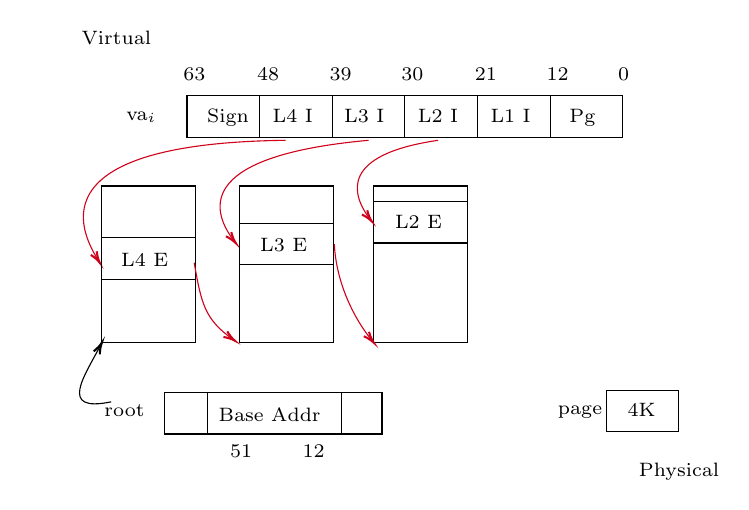
\begin{tikzpicture}[x=0.75pt,y=0.75pt,yscale=-0.5,xscale=0.5]
%uncomment if require: \path (0,462); %set diagram left start at 0, and has height of 462

%Shape: Rectangle [id:dp6123242987475281] 
\draw   (34,165) -- (124,165) -- (124,316) -- (34,316) -- cycle ;
%Shape: Rectangle [id:dp7959502838133716] 
\draw   (167,165) -- (257,165) -- (257,316) -- (167,316) -- cycle ;
%Shape: Rectangle [id:dp8145808612650314] 
\draw   (296,165) -- (386,165) -- (386,316) -- (296,316) -- cycle ;
%Shape: Rectangle [id:dp09188981629965576] 
\draw   (116,78) -- (186,78) -- (186,118) -- (116,118) -- cycle ;
%Shape: Rectangle [id:dp37293072339083944] 
\draw   (186,78) -- (256,78) -- (256,118) -- (186,118) -- cycle ;
%Shape: Rectangle [id:dp5793497397936833] 
\draw   (256,78) -- (326,78) -- (326,118) -- (256,118) -- cycle ;
%Shape: Rectangle [id:dp03642830368170813] 
\draw   (326,78) -- (396,78) -- (396,118) -- (326,118) -- cycle ;
%Shape: Rectangle [id:dp3584613533590697] 
\draw   (396,78) -- (466,78) -- (466,118) -- (396,118) -- cycle ;
%Shape: Rectangle [id:dp49270882304200136] 
\draw   (466,78) -- (536,78) -- (536,118) -- (466,118) -- cycle ;
%Curve Lines [id:da0504323435289209] 
\draw [color={rgb, 255:red, 208; green, 2; blue, 27 }  ,draw opacity=1 ]   (211,121) .. controls (-36.94,123.94) and (16.69,214.28) .. (31.17,237.65) ;
\draw [shift={(32,239)}, rotate = 238.24] [color={rgb, 255:red, 208; green, 2; blue, 27 }  ,draw opacity=1 ][line width=0.75]    (10.93,-3.29) .. controls (6.95,-1.4) and (3.31,-0.3) .. (0,0) .. controls (3.31,0.3) and (6.95,1.4) .. (10.93,3.29)   ;
%Shape: Rectangle [id:dp4075437908176933] 
\draw   (34,215) -- (124,215) -- (124,255) -- (34,255) -- cycle ;
%Curve Lines [id:da7050393599796472] 
\draw [color={rgb, 255:red, 208; green, 2; blue, 27 }  ,draw opacity=1 ]   (291,121) .. controls (117.54,136.68) and (141.92,192.7) .. (161.79,218.46) ;
\draw [shift={(163,220)}, rotate = 231.34] [color={rgb, 255:red, 208; green, 2; blue, 27 }  ,draw opacity=1 ][line width=0.75]    (10.93,-3.29) .. controls (6.95,-1.4) and (3.31,-0.3) .. (0,0) .. controls (3.31,0.3) and (6.95,1.4) .. (10.93,3.29)   ;
%Shape: Rectangle [id:dp5816879611235295] 
\draw   (167,201) -- (257,201) -- (257,241) -- (167,241) -- cycle ;
%Shape: Rectangle [id:dp18857932874079686] 
\draw   (296,180) -- (386,180) -- (386,220) -- (296,220) -- cycle ;
%Curve Lines [id:da4249233852783898] 
\draw [color={rgb, 255:red, 208; green, 2; blue, 27 }  ,draw opacity=1 ]   (358,121) .. controls (263.92,134.72) and (273.56,172.45) .. (292.81,197.48) ;
\draw [shift={(294,199)}, rotate = 231.34] [color={rgb, 255:red, 208; green, 2; blue, 27 }  ,draw opacity=1 ][line width=0.75]    (10.93,-3.29) .. controls (6.95,-1.4) and (3.31,-0.3) .. (0,0) .. controls (3.31,0.3) and (6.95,1.4) .. (10.93,3.29)   ;
%Curve Lines [id:da4304225854478958] 
\draw    (43,373) .. controls (-9.21,383.84) and (18.15,347.13) .. (33.32,317.36) ;
\draw [shift={(34,316)}, rotate = 116.57] [color={rgb, 255:red, 0; green, 0; blue, 0 }  ][line width=0.75]    (10.93,-3.29) .. controls (6.95,-1.4) and (3.31,-0.3) .. (0,0) .. controls (3.31,0.3) and (6.95,1.4) .. (10.93,3.29)   ;
%Curve Lines [id:da4757832236434707] 
\draw [color={rgb, 255:red, 208; green, 2; blue, 27 }  ,draw opacity=1 ]   (123,239) .. controls (129.9,278.4) and (132.91,293.54) .. (160.71,313.1) ;
\draw [shift={(162,314)}, rotate = 214.59] [color={rgb, 255:red, 208; green, 2; blue, 27 }  ,draw opacity=1 ][line width=0.75]    (10.93,-3.29) .. controls (6.95,-1.4) and (3.31,-0.3) .. (0,0) .. controls (3.31,0.3) and (6.95,1.4) .. (10.93,3.29)   ;
%Curve Lines [id:da31749049142629926] 
\draw [color={rgb, 255:red, 208; green, 2; blue, 27 }  ,draw opacity=1 ]   (258,221) .. controls (259.95,260) and (278.06,294.25) .. (294.72,314.47) ;
\draw [shift={(296,316)}, rotate = 229.64] [color={rgb, 255:red, 208; green, 2; blue, 27 }  ,draw opacity=1 ][line width=0.75]    (10.93,-3.29) .. controls (6.95,-1.4) and (3.31,-0.3) .. (0,0) .. controls (3.31,0.3) and (6.95,1.4) .. (10.93,3.29)   ;
%Shape: Rectangle [id:dp9593685170876407] 
\draw   (520,362) -- (590,362) -- (590,402) -- (520,402) -- cycle ;
%Shape: Rectangle [id:dp4782901135534001] 
\draw   (94,364) -- (135.5,364) -- (135.5,404) -- (94,404) -- cycle ;
%Shape: Rectangle [id:dp3063155121688097] 
\draw   (135.5,364) -- (264.5,364) -- (264.5,404) -- (135.5,404) -- cycle ;
%Shape: Rectangle [id:dp4595718689908179] 
\draw   (264.5,364) -- (304,364) -- (304,404) -- (264.5,404) -- cycle ;

% Text Node
\draw (12,13) node [anchor=north west][inner sep=0.75pt]   [align=left] {{\scriptsize Virtual}};
% Text Node
\draw (549,429) node [anchor=north west][inner sep=0.75pt]   [align=left] {{\scriptsize Physical}};
% Text Node
\draw (133,89) node [anchor=north west][inner sep=0.75pt]   [align=left] {{\scriptsize Sign}};
% Text Node
\draw (196,89) node [anchor=north west][inner sep=0.75pt]   [align=left] {{\scriptsize L4 I}};
% Text Node
\draw (265,89) node [anchor=north west][inner sep=0.75pt]   [align=left] {{\scriptsize L3 I}};
% Text Node
\draw (336,89) node [anchor=north west][inner sep=0.75pt]   [align=left] {{\scriptsize L2 I}};
% Text Node
\draw (406,89) node [anchor=north west][inner sep=0.75pt]   [align=left] {{\scriptsize L1 I}};
% Text Node
\draw (482,89) node [anchor=north west][inner sep=0.75pt]   [align=left] {{\scriptsize Pg}};
% Text Node
\draw (55,91) node [anchor=north west][inner sep=0.75pt]   [align=left] {{\scriptsize va$_i$}};
% Text Node
\draw (34,373) node [anchor=north west][inner sep=0.75pt]   [align=left] {{\scriptsize root}};
% Text Node
\draw (50,227) node [anchor=north west][inner sep=0.75pt]   [align=left] {{\scriptsize L4 E}};
% Text Node
\draw (184,213) node [anchor=north west][inner sep=0.75pt]   [align=left] {{\scriptsize L3 E}};
% Text Node
\draw (314,191) node [anchor=north west][inner sep=0.75pt]   [align=left] {{\scriptsize L2 E}};
% Text Node
\draw (471,375) node [anchor=north west][inner sep=0.75pt]   [align=left] {{\scriptsize page}};
% Text Node
\draw (538,372) node [anchor=north west][inner sep=0.75pt]   [align=left] {{\scriptsize 4K}};
% Text Node
\draw (155,412) node [anchor=north west][inner sep=0.75pt]   [align=left] {{\scriptsize 51}};
% Text Node
\draw (225,412) node [anchor=north west][inner sep=0.75pt]   [align=left] {{\scriptsize 12}};
% Text Node
\draw (144,376) node [anchor=north west][inner sep=0.75pt]   [align=left] {{\scriptsize Base Addr}};
% Text Node
\draw (110,49) node [anchor=north west][inner sep=0.75pt]   [align=left] {{\scriptsize 63}};
% Text Node
\draw (181,49) node [anchor=north west][inner sep=0.75pt]   [align=left] {{\scriptsize 48}};
% Text Node
\draw (251,49) node [anchor=north west][inner sep=0.75pt]   [align=left] {{\scriptsize 39}};
% Text Node
\draw (320,49) node [anchor=north west][inner sep=0.75pt]   [align=left] {{\scriptsize 30}};
% Text Node
\draw (391,49) node [anchor=north west][inner sep=0.75pt]   [align=left] {{\scriptsize 21}};
% Text Node
\draw (460,49) node [anchor=north west][inner sep=0.75pt]   [align=left] {{\scriptsize 12}};
% Text Node
\draw (529,49) node [anchor=north west][inner sep=0.75pt]   [align=left] {{\scriptsize 0}};


\end{tikzpicture}
        \caption{A New L2 Entry}
        \label{fig:enter-label}
    \end{figure}
    \column{.4\textwidth}
\begin{lstlisting}[style=CStyleNum, basicstyle=\tiny]
static pte_t *pte_nxt_table (pte_t *entry){
 pte_t *next;
 // If not already present, try to allocate
 if (!entry->present){
  if (!pte_alloc(&next)) {
   return NULL;
  }
  entry->pfn = PTE_PFN((uintptr_t) next);
  entry->present = 1;
  } else {
   uintptr_t next_phys_addr = PTE_PFN_TO_ADDR(entry->pfn);        
   uintptr_t next_virt_addr = (uintptr_t) P2V(next_phys_addr);
   next = (pte_t *) next_virt_addr;
  }
  return next;
}   
pte_t *walkpgdir(pte_t *l4, void *va){ 
 pte_t *l4_entry = &l4[L4I(va)];
 pte_t *l3 = pte_nxt_table(l4_entry);
 pte_t *l3_entry = &l3[L3I(va)];
 pte_t *l2 = pte_nxt_table(l3_entry);
 pte_t *l2_entry = &l3[L2I(va)];
}

\end{lstlisting}
\end{columns}
\end{frame}
%11---------------------------------------------------------------
\begin{frame}[fragile]{Sharing Physical Page Tables}
\begin{columns}[c]
\column{.59\textwidth}    
    \begin{figure}
        \centering
    \tikzset{every picture/.style={line width=0.75pt}} %set default line width to 0.75pt        
    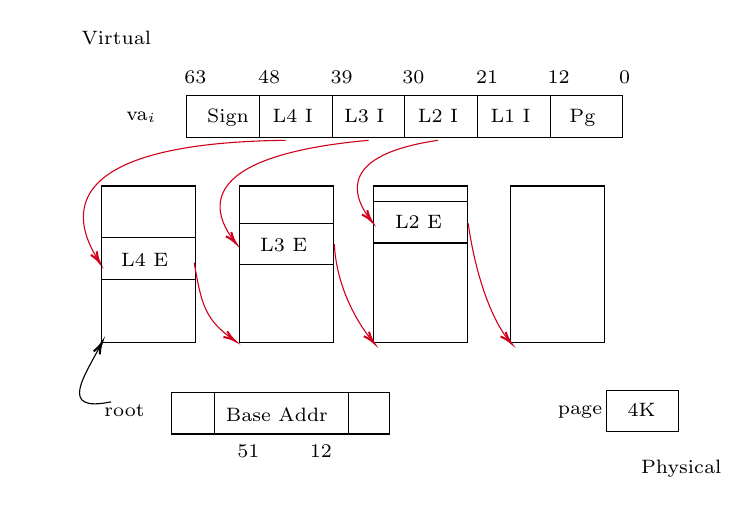
\begin{tikzpicture}[x=0.75pt,y=0.75pt,yscale=-0.5,xscale=0.5]
%uncomment if require: \path (0,461); %set diagram left start at 0, and has height of 461

%Shape: Rectangle [id:dp8985266189265282] 
\draw   (30,162) -- (120,162) -- (120,313) -- (30,313) -- cycle ;
%Shape: Rectangle [id:dp8580905480423404] 
\draw   (163,162) -- (253,162) -- (253,313) -- (163,313) -- cycle ;
%Shape: Rectangle [id:dp04681279805293914] 
\draw   (292,162) -- (382,162) -- (382,313) -- (292,313) -- cycle ;
%Shape: Rectangle [id:dp7764939174959982] 
\draw   (424,162) -- (514,162) -- (514,313) -- (424,313) -- cycle ;
%Shape: Rectangle [id:dp5300844634901585] 
\draw   (112,75) -- (182,75) -- (182,115) -- (112,115) -- cycle ;
%Shape: Rectangle [id:dp4415280160774133] 
\draw   (182,75) -- (252,75) -- (252,115) -- (182,115) -- cycle ;
%Shape: Rectangle [id:dp2994535835985157] 
\draw   (252,75) -- (322,75) -- (322,115) -- (252,115) -- cycle ;
%Shape: Rectangle [id:dp32418137012170356] 
\draw   (322,75) -- (392,75) -- (392,115) -- (322,115) -- cycle ;
%Shape: Rectangle [id:dp37951844906888543] 
\draw   (392,75) -- (462,75) -- (462,115) -- (392,115) -- cycle ;
%Shape: Rectangle [id:dp6243329849126165] 
\draw   (462,75) -- (532,75) -- (532,115) -- (462,115) -- cycle ;
%Curve Lines [id:da5300291149539194] 
\draw [color={rgb, 255:red, 208; green, 2; blue, 27 }  ,draw opacity=1 ]   (207,118) .. controls (-40.94,120.94) and (12.69,211.28) .. (27.17,234.65) ;
\draw [shift={(28,236)}, rotate = 238.24] [color={rgb, 255:red, 208; green, 2; blue, 27 }  ,draw opacity=1 ][line width=0.75]    (10.93,-3.29) .. controls (6.95,-1.4) and (3.31,-0.3) .. (0,0) .. controls (3.31,0.3) and (6.95,1.4) .. (10.93,3.29)   ;
%Shape: Rectangle [id:dp6164472725736567] 
\draw   (30,212) -- (120,212) -- (120,252) -- (30,252) -- cycle ;
%Curve Lines [id:da23035098640096874] 
\draw [color={rgb, 255:red, 208; green, 2; blue, 27 }  ,draw opacity=1 ]   (287,118) .. controls (113.54,133.68) and (137.92,189.7) .. (157.79,215.46) ;
\draw [shift={(159,217)}, rotate = 231.34] [color={rgb, 255:red, 208; green, 2; blue, 27 }  ,draw opacity=1 ][line width=0.75]    (10.93,-3.29) .. controls (6.95,-1.4) and (3.31,-0.3) .. (0,0) .. controls (3.31,0.3) and (6.95,1.4) .. (10.93,3.29)   ;
%Shape: Rectangle [id:dp6844649352396941] 
\draw   (163,198) -- (253,198) -- (253,238) -- (163,238) -- cycle ;
%Shape: Rectangle [id:dp14248498609413196] 
\draw   (292,177) -- (382,177) -- (382,217) -- (292,217) -- cycle ;
%Curve Lines [id:da681101715887759] 
\draw [color={rgb, 255:red, 208; green, 2; blue, 27 }  ,draw opacity=1 ]   (354,118) .. controls (259.92,131.72) and (269.56,169.45) .. (288.81,194.48) ;
\draw [shift={(290,196)}, rotate = 231.34] [color={rgb, 255:red, 208; green, 2; blue, 27 }  ,draw opacity=1 ][line width=0.75]    (10.93,-3.29) .. controls (6.95,-1.4) and (3.31,-0.3) .. (0,0) .. controls (3.31,0.3) and (6.95,1.4) .. (10.93,3.29)   ;
%Curve Lines [id:da7448745938095696] 
\draw    (39,370) .. controls (-13.21,380.84) and (14.15,344.13) .. (29.32,314.36) ;
\draw [shift={(30,313)}, rotate = 116.57] [color={rgb, 255:red, 0; green, 0; blue, 0 }  ][line width=0.75]    (10.93,-3.29) .. controls (6.95,-1.4) and (3.31,-0.3) .. (0,0) .. controls (3.31,0.3) and (6.95,1.4) .. (10.93,3.29)   ;
%Curve Lines [id:da22392385009085425] 
\draw [color={rgb, 255:red, 208; green, 2; blue, 27 }  ,draw opacity=1 ]   (119,236) .. controls (125.9,275.4) and (128.91,290.54) .. (156.71,310.1) ;
\draw [shift={(158,311)}, rotate = 214.59] [color={rgb, 255:red, 208; green, 2; blue, 27 }  ,draw opacity=1 ][line width=0.75]    (10.93,-3.29) .. controls (6.95,-1.4) and (3.31,-0.3) .. (0,0) .. controls (3.31,0.3) and (6.95,1.4) .. (10.93,3.29)   ;
%Curve Lines [id:da7384001101529021] 
\draw [color={rgb, 255:red, 208; green, 2; blue, 27 }  ,draw opacity=1 ]   (254,218) .. controls (255.95,257) and (274.06,291.25) .. (290.72,311.47) ;
\draw [shift={(292,313)}, rotate = 229.64] [color={rgb, 255:red, 208; green, 2; blue, 27 }  ,draw opacity=1 ][line width=0.75]    (10.93,-3.29) .. controls (6.95,-1.4) and (3.31,-0.3) .. (0,0) .. controls (3.31,0.3) and (6.95,1.4) .. (10.93,3.29)   ;
%Curve Lines [id:da461641424558785] 
\draw [color={rgb, 255:red, 208; green, 2; blue, 27 }  ,draw opacity=1 ]   (383,198) .. controls (389.86,247) and (405.36,291.2) .. (422.92,311.77) ;
\draw [shift={(424,313)}, rotate = 228.01] [color={rgb, 255:red, 208; green, 2; blue, 27 }  ,draw opacity=1 ][line width=0.75]    (10.93,-3.29) .. controls (6.95,-1.4) and (3.31,-0.3) .. (0,0) .. controls (3.31,0.3) and (6.95,1.4) .. (10.93,3.29)   ;
%Shape: Rectangle [id:dp7456876017683469] 
\draw   (516,359) -- (586,359) -- (586,399) -- (516,399) -- cycle ;
%Shape: Rectangle [id:dp44145929649929916] 
\draw   (97,361) -- (138.5,361) -- (138.5,401) -- (97,401) -- cycle ;
%Shape: Rectangle [id:dp6608975412508127] 
\draw   (138.5,361) -- (267.5,361) -- (267.5,401) -- (138.5,401) -- cycle ;
%Shape: Rectangle [id:dp927545333863445] 
\draw   (267.5,361) -- (307,361) -- (307,401) -- (267.5,401) -- cycle ;

% Text Node
\draw (8,10) node [anchor=north west][inner sep=0.75pt]   [align=left] {{\scriptsize Virtual}};
% Text Node
\draw (547,424) node [anchor=north west][inner sep=0.75pt]   [align=left] {{\scriptsize Physical}};
% Text Node
\draw (129,86) node [anchor=north west][inner sep=0.75pt]   [align=left] {{\scriptsize Sign}};
% Text Node
\draw (192,86) node [anchor=north west][inner sep=0.75pt]   [align=left] {{\scriptsize L4 I}};
% Text Node
\draw (261,86) node [anchor=north west][inner sep=0.75pt]   [align=left] {{\scriptsize L3 I}};
% Text Node
\draw (332,86) node [anchor=north west][inner sep=0.75pt]   [align=left] {{\scriptsize L2 I}};
% Text Node
\draw (402,86) node [anchor=north west][inner sep=0.75pt]   [align=left] {{\scriptsize L1 I}};
% Text Node
\draw (478,86) node [anchor=north west][inner sep=0.75pt]   [align=left] {{\scriptsize Pg}};
% Text Node
\draw (51,88) node [anchor=north west][inner sep=0.75pt]   [align=left] {{\scriptsize va$_i$}};
% Text Node
\draw (30,370) node [anchor=north west][inner sep=0.75pt]   [align=left] {{\scriptsize root}};
% Text Node
\draw (46,224) node [anchor=north west][inner sep=0.75pt]   [align=left] {{\scriptsize L4 E}};
% Text Node
\draw (180,210) node [anchor=north west][inner sep=0.75pt]   [align=left] {{\scriptsize L3 E}};
% Text Node
\draw (310,188) node [anchor=north west][inner sep=0.75pt]   [align=left] {{\scriptsize L2 E}};
% Text Node
\draw (467,372) node [anchor=north west][inner sep=0.75pt]   [align=left] {{\scriptsize page}};
% Text Node
\draw (534,369) node [anchor=north west][inner sep=0.75pt]   [align=left] {{\scriptsize 4K}};
% Text Node
\draw (158,409) node [anchor=north west][inner sep=0.75pt]   [align=left] {{\scriptsize 51}};
% Text Node
\draw (228,409) node [anchor=north west][inner sep=0.75pt]   [align=left] {{\scriptsize 12}};
% Text Node
\draw (147,373) node [anchor=north west][inner sep=0.75pt]   [align=left] {{\scriptsize Base Addr}};
% Text Node
\draw (107,49) node [anchor=north west][inner sep=0.75pt]   [align=left] {{\scriptsize 63}};
% Text Node
\draw (178,49) node [anchor=north west][inner sep=0.75pt]   [align=left] {{\scriptsize 48}};
% Text Node
\draw (248,49) node [anchor=north west][inner sep=0.75pt]   [align=left] {{\scriptsize 39}};
% Text Node
\draw (317,49) node [anchor=north west][inner sep=0.75pt]   [align=left] {{\scriptsize 30}};
% Text Node
\draw (388,49) node [anchor=north west][inner sep=0.75pt]   [align=left] {{\scriptsize 21}};
% Text Node
\draw (457,49) node [anchor=north west][inner sep=0.75pt]   [align=left] {{\scriptsize 12}};
% Text Node
\draw (526,49) node [anchor=north west][inner sep=0.75pt]   [align=left] {{\scriptsize 0}};


\end{tikzpicture}
        \caption{Accessing L1 Table}
        \label{fig:enter-label}
    \end{figure}
    \column{.4\textwidth}
\begin{lstlisting}[style=CStyleNum, basicstyle=\tiny]
static pte_t *pte_nxt_table (pte_t *entry){
 pte_t *next;
 // If not already present, try to allocate
 if (!entry->present){
  if (!pte_alloc(&next)) {
   return NULL;
  }
  entry->pfn = PTE_PFN((uintptr_t) next);
  entry->present = 1;
  } else {
   uintptr_t next_phys_addr = PTE_PFN_TO_ADDR(entry->pfn);        
   uintptr_t next_virt_addr = (uintptr_t) P2V(next_phys_addr);
   next = (pte_t *) next_virt_addr;
  }
  return next;
}   
pte_t *walkpgdir(pte_t *l4, void *va){ 
 pte_t *l4_entry = &l4[L4I(va)];
 pte_t *l3 = pte_nxt_table(l4_entry);
 pte_t *l3_entry = &l3[L3I(va)];
 pte_t *l2 = pte_nxt_table(l3_entry);
 pte_t *l2_entry = &l3[L2I(va)];  
 pte_t *l1 = pte_nxt_table(l2_entry);
}

\end{lstlisting}
\end{columns}
\end{frame}
%12------------------------------------------------------------
\begin{frame}[fragile]{Sharing Physical Page Tables}
\begin{columns}[c]
\column{.59\textwidth}    
    \begin{figure}
        \centering
        
\tikzset{every picture/.style={line width=0.75pt}} %set default line width to 0.75pt        

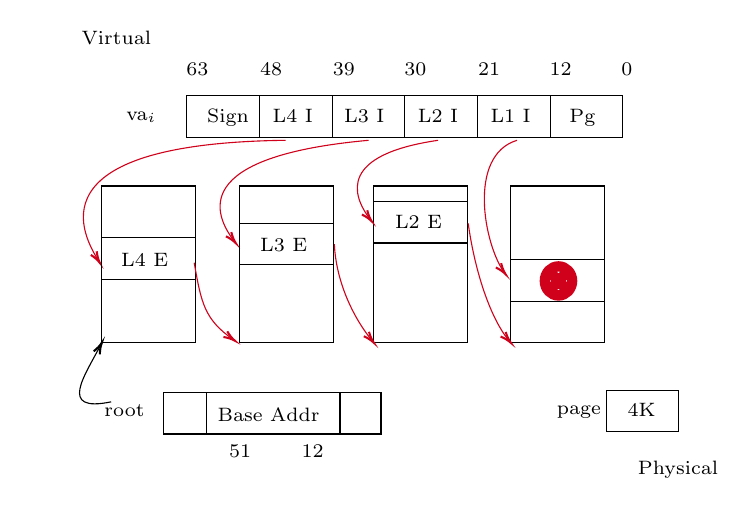
\begin{tikzpicture}[x=0.75pt,y=0.75pt,yscale=-0.5,xscale=0.5]
%uncomment if require: \path (0,471); %set diagram left start at 0, and has height of 471

%Shape: Rectangle [id:dp8920944025204927] 
\draw   (38,170) -- (128,170) -- (128,321) -- (38,321) -- cycle ;
%Shape: Rectangle [id:dp8039737032506988] 
\draw   (171,170) -- (261,170) -- (261,321) -- (171,321) -- cycle ;
%Shape: Rectangle [id:dp42908346405019016] 
\draw   (300,170) -- (390,170) -- (390,321) -- (300,321) -- cycle ;
%Shape: Rectangle [id:dp8197691504489653] 
\draw   (432,170) -- (522,170) -- (522,321) -- (432,321) -- cycle ;
%Shape: Rectangle [id:dp1292469982220843] 
\draw   (120,83) -- (190,83) -- (190,123) -- (120,123) -- cycle ;
%Shape: Rectangle [id:dp17292447138779332] 
\draw   (190,83) -- (260,83) -- (260,123) -- (190,123) -- cycle ;
%Shape: Rectangle [id:dp2994041750049934] 
\draw   (260,83) -- (330,83) -- (330,123) -- (260,123) -- cycle ;
%Shape: Rectangle [id:dp6558969947689828] 
\draw   (330,83) -- (400,83) -- (400,123) -- (330,123) -- cycle ;
%Shape: Rectangle [id:dp8919322560991858] 
\draw   (400,83) -- (470,83) -- (470,123) -- (400,123) -- cycle ;
%Shape: Rectangle [id:dp16287367514319318] 
\draw   (470,83) -- (540,83) -- (540,123) -- (470,123) -- cycle ;
%Curve Lines [id:da8252306127206739] 
\draw [color={rgb, 255:red, 208; green, 2; blue, 27 }  ,draw opacity=1 ]   (215,126) .. controls (-32.94,128.94) and (20.69,219.28) .. (35.17,242.65) ;
\draw [shift={(36,244)}, rotate = 238.24] [color={rgb, 255:red, 208; green, 2; blue, 27 }  ,draw opacity=1 ][line width=0.75]    (10.93,-3.29) .. controls (6.95,-1.4) and (3.31,-0.3) .. (0,0) .. controls (3.31,0.3) and (6.95,1.4) .. (10.93,3.29)   ;
%Shape: Rectangle [id:dp8056804187093134] 
\draw   (38,220) -- (128,220) -- (128,260) -- (38,260) -- cycle ;
%Curve Lines [id:da41594618161660457] 
\draw [color={rgb, 255:red, 208; green, 2; blue, 27 }  ,draw opacity=1 ]   (295,126) .. controls (121.54,141.68) and (145.92,197.7) .. (165.79,223.46) ;
\draw [shift={(167,225)}, rotate = 231.34] [color={rgb, 255:red, 208; green, 2; blue, 27 }  ,draw opacity=1 ][line width=0.75]    (10.93,-3.29) .. controls (6.95,-1.4) and (3.31,-0.3) .. (0,0) .. controls (3.31,0.3) and (6.95,1.4) .. (10.93,3.29)   ;
%Shape: Rectangle [id:dp16557950449596315] 
\draw   (171,206) -- (261,206) -- (261,246) -- (171,246) -- cycle ;
%Shape: Rectangle [id:dp34877861725129655] 
\draw   (300,185) -- (390,185) -- (390,225) -- (300,225) -- cycle ;
%Shape: Rectangle [id:dp3058228778549279] 
\draw   (432,241) -- (522,241) -- (522,281) -- (432,281) -- cycle ;
%Curve Lines [id:da3826636793573912] 
\draw [color={rgb, 255:red, 208; green, 2; blue, 27 }  ,draw opacity=1 ]   (362,126) .. controls (267.92,139.72) and (277.56,177.45) .. (296.81,202.48) ;
\draw [shift={(298,204)}, rotate = 231.34] [color={rgb, 255:red, 208; green, 2; blue, 27 }  ,draw opacity=1 ][line width=0.75]    (10.93,-3.29) .. controls (6.95,-1.4) and (3.31,-0.3) .. (0,0) .. controls (3.31,0.3) and (6.95,1.4) .. (10.93,3.29)   ;
%Curve Lines [id:da5001726543329206] 
\draw [color={rgb, 255:red, 208; green, 2; blue, 27 }  ,draw opacity=1 ]   (438,126) .. controls (389.98,140.7) and (406.31,226.47) .. (425.8,253.42) ;
\draw [shift={(427,255)}, rotate = 231.34] [color={rgb, 255:red, 208; green, 2; blue, 27 }  ,draw opacity=1 ][line width=0.75]    (10.93,-3.29) .. controls (6.95,-1.4) and (3.31,-0.3) .. (0,0) .. controls (3.31,0.3) and (6.95,1.4) .. (10.93,3.29)   ;
%Curve Lines [id:da631836674879221] 
\draw    (47,378) .. controls (-5.21,388.84) and (22.15,352.13) .. (37.32,322.36) ;
\draw [shift={(38,321)}, rotate = 116.57] [color={rgb, 255:red, 0; green, 0; blue, 0 }  ][line width=0.75]    (10.93,-3.29) .. controls (6.95,-1.4) and (3.31,-0.3) .. (0,0) .. controls (3.31,0.3) and (6.95,1.4) .. (10.93,3.29)   ;
%Curve Lines [id:da3186235321456783] 
\draw [color={rgb, 255:red, 208; green, 2; blue, 27 }  ,draw opacity=1 ]   (127,244) .. controls (133.9,283.4) and (136.91,298.54) .. (164.71,318.1) ;
\draw [shift={(166,319)}, rotate = 214.59] [color={rgb, 255:red, 208; green, 2; blue, 27 }  ,draw opacity=1 ][line width=0.75]    (10.93,-3.29) .. controls (6.95,-1.4) and (3.31,-0.3) .. (0,0) .. controls (3.31,0.3) and (6.95,1.4) .. (10.93,3.29)   ;
%Curve Lines [id:da8367405116543691] 
\draw [color={rgb, 255:red, 208; green, 2; blue, 27 }  ,draw opacity=1 ]   (262,226) .. controls (263.95,265) and (282.06,299.25) .. (298.72,319.47) ;
\draw [shift={(300,321)}, rotate = 229.64] [color={rgb, 255:red, 208; green, 2; blue, 27 }  ,draw opacity=1 ][line width=0.75]    (10.93,-3.29) .. controls (6.95,-1.4) and (3.31,-0.3) .. (0,0) .. controls (3.31,0.3) and (6.95,1.4) .. (10.93,3.29)   ;
%Curve Lines [id:da5457897242691585] 
\draw [color={rgb, 255:red, 208; green, 2; blue, 27 }  ,draw opacity=1 ]   (391,206) .. controls (397.86,255) and (413.36,299.2) .. (430.92,319.77) ;
\draw [shift={(432,321)}, rotate = 228.01] [color={rgb, 255:red, 208; green, 2; blue, 27 }  ,draw opacity=1 ][line width=0.75]    (10.93,-3.29) .. controls (6.95,-1.4) and (3.31,-0.3) .. (0,0) .. controls (3.31,0.3) and (6.95,1.4) .. (10.93,3.29)   ;
%Shape: Rectangle [id:dp10581044847356069] 
\draw   (524,367) -- (594,367) -- (594,407) -- (524,407) -- cycle ;
%Shape: Rectangle [id:dp3288182618410409] 
\draw   (97,369) -- (138.5,369) -- (138.5,409) -- (97,409) -- cycle ;
%Shape: Rectangle [id:dp9351470025119926] 
\draw   (138.5,369) -- (267.5,369) -- (267.5,409) -- (138.5,409) -- cycle ;
%Shape: Rectangle [id:dp9896731702970194] 
\draw   (267.5,369) -- (307,369) -- (307,409) -- (267.5,409) -- cycle ;
%Shape: Light Bulb [id:dp8297924129311762] 
\draw  [color={rgb, 255:red, 208; green, 2; blue, 27 }  ,draw opacity=1 ][line width=3.75]  (464.88,261.5) .. controls (464.88,253.77) and (470.75,247.5) .. (478,247.5) .. controls (485.25,247.5) and (491.13,253.77) .. (491.13,261.5) .. controls (491.13,269.23) and (485.25,275.5) .. (478,275.5) .. controls (470.75,275.5) and (464.88,269.23) .. (464.88,261.5) -- cycle (468.66,251.53) -- (487.35,271.47) (487.35,251.53) -- (468.66,271.47) (462.25,261.5) -- (464.88,261.5) (491.13,261.5) -- (493.75,261.5) ;

% Text Node
\draw (16,18) node [anchor=north west][inner sep=0.75pt]   [align=left] {{\scriptsize Virtual}};
% Text Node
\draw (552,433) node [anchor=north west][inner sep=0.75pt]   [align=left] {{\scriptsize Physical}};
% Text Node
\draw (137,94) node [anchor=north west][inner sep=0.75pt]   [align=left] {{\scriptsize Sign}};
% Text Node
\draw (200,94) node [anchor=north west][inner sep=0.75pt]   [align=left] {{\scriptsize L4 I}};
% Text Node
\draw (269,94) node [anchor=north west][inner sep=0.75pt]   [align=left] {{\scriptsize L3 I}};
% Text Node
\draw (340,94) node [anchor=north west][inner sep=0.75pt]   [align=left] {{\scriptsize L2 I}};
% Text Node
\draw (410,94) node [anchor=north west][inner sep=0.75pt]   [align=left] {{\scriptsize L1 I}};
% Text Node
\draw (486,94) node [anchor=north west][inner sep=0.75pt]   [align=left] {{\scriptsize Pg}};
% Text Node
\draw (59,96) node [anchor=north west][inner sep=0.75pt]   [align=left] {{\scriptsize va$_i$}};
% Text Node
\draw (38,378) node [anchor=north west][inner sep=0.75pt]   [align=left] {{\scriptsize root}};
% Text Node
\draw (54,232) node [anchor=north west][inner sep=0.75pt]   [align=left] {{\scriptsize L4 E}};
% Text Node
\draw (188,218) node [anchor=north west][inner sep=0.75pt]   [align=left] {{\scriptsize L3 E}};
% Text Node
\draw (318,196) node [anchor=north west][inner sep=0.75pt]   [align=left] {{\scriptsize L2 E}};
% Text Node
\draw (474,380) node [anchor=north west][inner sep=0.75pt]   [align=left] {{\scriptsize page}};
% Text Node
\draw (542,377) node [anchor=north west][inner sep=0.75pt]   [align=left] {{\scriptsize 4K}};
% Text Node
\draw (158,417) node [anchor=north west][inner sep=0.75pt]   [align=left] {{\scriptsize 51}};
% Text Node
\draw (228,417) node [anchor=north west][inner sep=0.75pt]   [align=left] {{\scriptsize 12}};
% Text Node
\draw (147,381) node [anchor=north west][inner sep=0.75pt]   [align=left] {{\scriptsize Base Addr}};
% Text Node
\draw (117,49) node [anchor=north west][inner sep=0.75pt]   [align=left] {{\scriptsize 63}};
% Text Node
\draw (188,49) node [anchor=north west][inner sep=0.75pt]   [align=left] {{\scriptsize 48}};
% Text Node
\draw (258,49) node [anchor=north west][inner sep=0.75pt]   [align=left] {{\scriptsize 39}};
% Text Node
\draw (327,49) node [anchor=north west][inner sep=0.75pt]   [align=left] {{\scriptsize 30}};
% Text Node
\draw (398,49) node [anchor=north west][inner sep=0.75pt]   [align=left] {{\scriptsize 21}};
% Text Node
\draw (467,49) node [anchor=north west][inner sep=0.75pt]   [align=left] {{\scriptsize 12}};
% Text Node
\draw (536,49) node [anchor=north west][inner sep=0.75pt]   [align=left] {{\scriptsize 0}};


\end{tikzpicture}
        \caption{Missing L1 Entry}
        \label{fig:enter-label}
    \end{figure}
    \column{.4\textwidth}
\begin{lstlisting}[style=CStyleNum, basicstyle=\tiny]
static pte_t *pte_nxt_table (pte_t *entry){
 pte_t *next;
 // If not already present, try to allocate
 if (!entry->present){
  if (!pte_alloc(&next)) {
   return NULL;
  }
  entry->pfn = PTE_PFN((uintptr_t) next);
  entry->present = 1;
  } else {
   uintptr_t next_phys_addr = PTE_PFN_TO_ADDR(entry->pfn);        
   uintptr_t next_virt_addr = (uintptr_t) P2V(next_phys_addr);
   next = (pte_t *) next_virt_addr;
  }
  return next;
}   
pte_t *walkpgdir(pte_t *l4, void *va){ 
 pte_t *l4_entry = &l4[L4I(va)];
 pte_t *l3 = pte_nxt_table(l4_entry);
 pte_t *l3_entry = &l3[L3I(va)];
 pte_t *l2 = pte_nxt_table(l3_entry);
 pte_t *l2_entry = &l3[L2I(va)];  
 pte_t *l1 = pte_nxt_table(l2_entry);
}

\end{lstlisting}
\end{columns}
\end{frame}
%13--------------------------------------------------------
%14----------------------------------------------------------
\begin{frame}[fragile]{Sharing Physical Page Tables}
\begin{columns}[c]
\column{.59\textwidth}    
    \begin{figure}
        \centering
\tikzset{every picture/.style={line width=0.75pt}} %set default line width to 0.75pt        
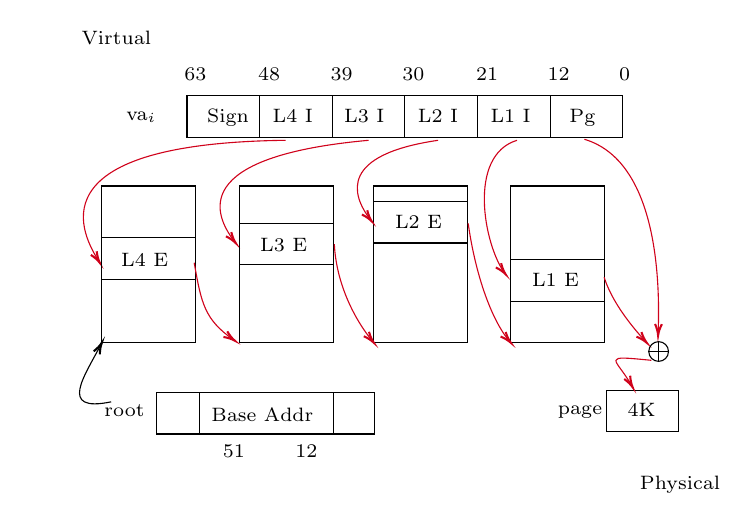
\begin{tikzpicture}[x=0.75pt,y=0.75pt,yscale=-0.5,xscale=0.5]
%uncomment if require: \path (0,471); %set diagram left start at 0, and has height of 471

%Shape: Rectangle [id:dp6797306099675045] 
\draw   (34,165) -- (124,165) -- (124,316) -- (34,316) -- cycle ;
%Shape: Rectangle [id:dp6192113478200691] 
\draw   (167,165) -- (257,165) -- (257,316) -- (167,316) -- cycle ;
%Shape: Rectangle [id:dp046479372017499854] 
\draw   (296,165) -- (386,165) -- (386,316) -- (296,316) -- cycle ;
%Shape: Rectangle [id:dp1806612887251846] 
\draw   (428,165) -- (518,165) -- (518,316) -- (428,316) -- cycle ;
%Shape: Rectangle [id:dp16201905390239735] 
\draw   (116,78) -- (186,78) -- (186,118) -- (116,118) -- cycle ;
%Shape: Rectangle [id:dp46359313115432044] 
\draw   (186,78) -- (256,78) -- (256,118) -- (186,118) -- cycle ;
%Shape: Rectangle [id:dp8986469180554777] 
\draw   (256,78) -- (326,78) -- (326,118) -- (256,118) -- cycle ;
%Shape: Rectangle [id:dp3960250568381902] 
\draw   (326,78) -- (396,78) -- (396,118) -- (326,118) -- cycle ;
%Shape: Rectangle [id:dp76786771788994] 
\draw   (396,78) -- (466,78) -- (466,118) -- (396,118) -- cycle ;
%Shape: Rectangle [id:dp9070245370995538] 
\draw   (466,78) -- (536,78) -- (536,118) -- (466,118) -- cycle ;
%Curve Lines [id:da6951218383977624] 
\draw [color={rgb, 255:red, 208; green, 2; blue, 27 }  ,draw opacity=1 ]   (211,121) .. controls (-36.94,123.94) and (16.69,214.28) .. (31.17,237.65) ;
\draw [shift={(32,239)}, rotate = 238.24] [color={rgb, 255:red, 208; green, 2; blue, 27 }  ,draw opacity=1 ][line width=0.75]    (10.93,-3.29) .. controls (6.95,-1.4) and (3.31,-0.3) .. (0,0) .. controls (3.31,0.3) and (6.95,1.4) .. (10.93,3.29)   ;
%Shape: Rectangle [id:dp48687197518810277] 
\draw   (34,215) -- (124,215) -- (124,255) -- (34,255) -- cycle ;
%Curve Lines [id:da7139570096435448] 
\draw [color={rgb, 255:red, 208; green, 2; blue, 27 }  ,draw opacity=1 ]   (291,121) .. controls (117.54,136.68) and (141.92,192.7) .. (161.79,218.46) ;
\draw [shift={(163,220)}, rotate = 231.34] [color={rgb, 255:red, 208; green, 2; blue, 27 }  ,draw opacity=1 ][line width=0.75]    (10.93,-3.29) .. controls (6.95,-1.4) and (3.31,-0.3) .. (0,0) .. controls (3.31,0.3) and (6.95,1.4) .. (10.93,3.29)   ;
%Shape: Rectangle [id:dp32338125663089956] 
\draw   (167,201) -- (257,201) -- (257,241) -- (167,241) -- cycle ;
%Shape: Rectangle [id:dp6104052627034173] 
\draw   (296,180) -- (386,180) -- (386,220) -- (296,220) -- cycle ;
%Shape: Rectangle [id:dp49476345634718477] 
\draw   (428,236) -- (518,236) -- (518,276) -- (428,276) -- cycle ;
%Curve Lines [id:da3926551025530285] 
\draw [color={rgb, 255:red, 208; green, 2; blue, 27 }  ,draw opacity=1 ]   (358,121) .. controls (263.92,134.72) and (273.56,172.45) .. (292.81,197.48) ;
\draw [shift={(294,199)}, rotate = 231.34] [color={rgb, 255:red, 208; green, 2; blue, 27 }  ,draw opacity=1 ][line width=0.75]    (10.93,-3.29) .. controls (6.95,-1.4) and (3.31,-0.3) .. (0,0) .. controls (3.31,0.3) and (6.95,1.4) .. (10.93,3.29)   ;
%Curve Lines [id:da38615138851194764] 
\draw [color={rgb, 255:red, 208; green, 2; blue, 27 }  ,draw opacity=1 ]   (434,121) .. controls (385.98,135.7) and (402.31,221.47) .. (421.8,248.42) ;
\draw [shift={(423,250)}, rotate = 231.34] [color={rgb, 255:red, 208; green, 2; blue, 27 }  ,draw opacity=1 ][line width=0.75]    (10.93,-3.29) .. controls (6.95,-1.4) and (3.31,-0.3) .. (0,0) .. controls (3.31,0.3) and (6.95,1.4) .. (10.93,3.29)   ;
%Curve Lines [id:da8796700124764012] 
\draw [color={rgb, 255:red, 208; green, 2; blue, 27 }  ,draw opacity=1 ]   (499,120) .. controls (574.46,142.54) and (571.17,273.61) .. (570.06,307.07) ;
\draw [shift={(570,309)}, rotate = 271.91] [color={rgb, 255:red, 208; green, 2; blue, 27 }  ,draw opacity=1 ][line width=0.75]    (10.93,-3.29) .. controls (6.95,-1.4) and (3.31,-0.3) .. (0,0) .. controls (3.31,0.3) and (6.95,1.4) .. (10.93,3.29)   ;
%Curve Lines [id:da26463336009584704] 
\draw    (43,373) .. controls (-9.21,383.84) and (18.15,347.13) .. (33.32,317.36) ;
\draw [shift={(34,316)}, rotate = 116.57] [color={rgb, 255:red, 0; green, 0; blue, 0 }  ][line width=0.75]    (10.93,-3.29) .. controls (6.95,-1.4) and (3.31,-0.3) .. (0,0) .. controls (3.31,0.3) and (6.95,1.4) .. (10.93,3.29)   ;
%Curve Lines [id:da18202057955172246] 
\draw [color={rgb, 255:red, 208; green, 2; blue, 27 }  ,draw opacity=1 ]   (123,239) .. controls (129.9,278.4) and (132.91,293.54) .. (160.71,313.1) ;
\draw [shift={(162,314)}, rotate = 214.59] [color={rgb, 255:red, 208; green, 2; blue, 27 }  ,draw opacity=1 ][line width=0.75]    (10.93,-3.29) .. controls (6.95,-1.4) and (3.31,-0.3) .. (0,0) .. controls (3.31,0.3) and (6.95,1.4) .. (10.93,3.29)   ;
%Curve Lines [id:da39925694981212034] 
\draw [color={rgb, 255:red, 208; green, 2; blue, 27 }  ,draw opacity=1 ]   (258,221) .. controls (259.95,260) and (278.06,294.25) .. (294.72,314.47) ;
\draw [shift={(296,316)}, rotate = 229.64] [color={rgb, 255:red, 208; green, 2; blue, 27 }  ,draw opacity=1 ][line width=0.75]    (10.93,-3.29) .. controls (6.95,-1.4) and (3.31,-0.3) .. (0,0) .. controls (3.31,0.3) and (6.95,1.4) .. (10.93,3.29)   ;
%Curve Lines [id:da0025982000064483923] 
\draw [color={rgb, 255:red, 208; green, 2; blue, 27 }  ,draw opacity=1 ]   (387,201) .. controls (393.86,250) and (409.36,294.2) .. (426.92,314.77) ;
\draw [shift={(428,316)}, rotate = 228.01] [color={rgb, 255:red, 208; green, 2; blue, 27 }  ,draw opacity=1 ][line width=0.75]    (10.93,-3.29) .. controls (6.95,-1.4) and (3.31,-0.3) .. (0,0) .. controls (3.31,0.3) and (6.95,1.4) .. (10.93,3.29)   ;
%Curve Lines [id:da4425456634879614] 
\draw [color={rgb, 255:red, 208; green, 2; blue, 27 }  ,draw opacity=1 ]   (518,253) .. controls (525.76,277.25) and (544.81,300.56) .. (557.81,314.71) ;
\draw [shift={(559,316)}, rotate = 227.12] [color={rgb, 255:red, 208; green, 2; blue, 27 }  ,draw opacity=1 ][line width=0.75]    (10.93,-3.29) .. controls (6.95,-1.4) and (3.31,-0.3) .. (0,0) .. controls (3.31,0.3) and (6.95,1.4) .. (10.93,3.29)   ;
%Shape: Rectangle [id:dp20590678105984384] 
\draw   (520,362) -- (590,362) -- (590,402) -- (520,402) -- cycle ;
%Shape: Rectangle [id:dp8145206670609288] 
\draw   (87,364) -- (128.5,364) -- (128.5,404) -- (87,404) -- cycle ;
%Shape: Rectangle [id:dp5322999267202655] 
\draw   (128.5,364) -- (257.5,364) -- (257.5,404) -- (128.5,404) -- cycle ;
%Shape: Rectangle [id:dp44035388924299834] 
\draw   (257.5,364) -- (297,364) -- (297,404) -- (257.5,404) -- cycle ;
\draw   (561,324.5) .. controls (561,319.25) and (565.25,315) .. (570.5,315) .. controls (575.75,315) and (580,319.25) .. (580,324.5) .. controls (580,329.75) and (575.75,334) .. (570.5,334) .. controls (565.25,334) and (561,329.75) .. (561,324.5) -- cycle ; \draw   (561,324.5) -- (580,324.5) ; \draw   (570.5,315) -- (570.5,334) ;
%Curve Lines [id:da7994290642535546] 
\draw [color={rgb, 255:red, 208; green, 2; blue, 27 }  ,draw opacity=1 ]   (563.5,333) .. controls (513.52,328.1) and (528.85,329.92) .. (544.54,357.29) ;
\draw [shift={(545.5,359)}, rotate = 241.11] [color={rgb, 255:red, 208; green, 2; blue, 27 }  ,draw opacity=1 ][line width=0.75]    (10.93,-3.29) .. controls (6.95,-1.4) and (3.31,-0.3) .. (0,0) .. controls (3.31,0.3) and (6.95,1.4) .. (10.93,3.29)   ;

% Text Node
\draw (12,13) node [anchor=north west][inner sep=0.75pt]   [align=left] {{\scriptsize Virtual}};
% Text Node
\draw (550,442) node [anchor=north west][inner sep=0.75pt]   [align=left] {{\scriptsize Physical}};
% Text Node
\draw (133,89) node [anchor=north west][inner sep=0.75pt]   [align=left] {{\scriptsize Sign}};
% Text Node
\draw (196,89) node [anchor=north west][inner sep=0.75pt]   [align=left] {{\scriptsize L4 I}};
% Text Node
\draw (265,89) node [anchor=north west][inner sep=0.75pt]   [align=left] {{\scriptsize L3 I}};
% Text Node
\draw (336,89) node [anchor=north west][inner sep=0.75pt]   [align=left] {{\scriptsize L2 I}};
% Text Node
\draw (406,89) node [anchor=north west][inner sep=0.75pt]   [align=left] {{\scriptsize L1 I}};
% Text Node
\draw (482,89) node [anchor=north west][inner sep=0.75pt]   [align=left] {{\scriptsize Pg}};
% Text Node
\draw (55,91) node [anchor=north west][inner sep=0.75pt]   [align=left] {{\scriptsize va$_i$}};
% Text Node
\draw (34,373) node [anchor=north west][inner sep=0.75pt]   [align=left] {{\scriptsize root}};
% Text Node
\draw (50,227) node [anchor=north west][inner sep=0.75pt]   [align=left] {{\scriptsize L4 E}};
% Text Node
\draw (184,213) node [anchor=north west][inner sep=0.75pt]   [align=left] {{\scriptsize L3 E}};
% Text Node
\draw (314,191) node [anchor=north west][inner sep=0.75pt]   [align=left] {{\scriptsize L2 E}};
% Text Node
\draw (446,247) node [anchor=north west][inner sep=0.75pt]   [align=left] {{\scriptsize L1 E}};
% Text Node
\draw (471,375) node [anchor=north west][inner sep=0.75pt]   [align=left] {{\scriptsize page}};
% Text Node
\draw (538,372) node [anchor=north west][inner sep=0.75pt]   [align=left] {{\scriptsize 4K}};
% Text Node
\draw (148,412) node [anchor=north west][inner sep=0.75pt]   [align=left] {{\scriptsize 51}};
% Text Node
\draw (218,412) node [anchor=north west][inner sep=0.75pt]   [align=left] {{\scriptsize 12}};
% Text Node
\draw (137,376) node [anchor=north west][inner sep=0.75pt]   [align=left] {{\scriptsize Base Addr}};
% Text Node
\draw (111,49) node [anchor=north west][inner sep=0.75pt]   [align=left] {{\scriptsize 63}};
% Text Node
\draw (182,49) node [anchor=north west][inner sep=0.75pt]   [align=left] {{\scriptsize 48}};
% Text Node
\draw (252,49) node [anchor=north west][inner sep=0.75pt]   [align=left] {{\scriptsize 39}};
% Text Node
\draw (321,49) node [anchor=north west][inner sep=0.75pt]   [align=left] {{\scriptsize 30}};
% Text Node
\draw (392,49) node [anchor=north west][inner sep=0.75pt]   [align=left] {{\scriptsize 21}};
% Text Node
\draw (461,49) node [anchor=north west][inner sep=0.75pt]   [align=left] {{\scriptsize 12}};
% Text Node
\draw (530,49) node [anchor=north west][inner sep=0.75pt]   [align=left] {{\scriptsize 0}};


\end{tikzpicture}
          \caption{Accessing to the Page Referenced by L1 Entry}
        \label{fig:enter-label}
    \end{figure}
    \column{.4\textwidth}
\begin{lstlisting}[style=CStyleNum, basicstyle=\tiny]
static pte_t *pte_nxt_table (pte_t *entry){
 pte_t *next;
 // If not already present, try to allocate
 if (!entry->present){
  if (!pte_alloc(&next)) {
   return NULL;
  }
  entry->pfn = PTE_PFN((uintptr_t) next);
  entry->present = 1;
  } else {
   uintptr_t next_phys_addr = PTE_PFN_TO_ADDR(entry->pfn);        
   uintptr_t next_virt_addr = (uintptr_t) P2V(next_phys_addr);
   next = (pte_t *) next_virt_addr;
  }
  return next;
}   
pte_t *walkpgdir(pte_t *l4, void *va){ 
 pte_t *l4_entry = &l4[L4I(va)];
 pte_t *l3 = pte_nxt_table(l4_entry);
 pte_t *l3_entry = &l3[L3I(va)];
 pte_t *l2 = pte_nxt_table(l3_entry);
 pte_t *l2_entry = &l2[L2I(va)];  
 pte_t *l1 = pte_nxt_table(l2_entry);
 pte_t *l1_entry = &l1[L1I(va)];  
 return l1_entry
}
\end{lstlisting}
\end{columns}
\end{frame}

%Soundness of Page Table Traversal
%--------------------------------------------
\begin{frame}{Breaking Soundness in Sharing}
    \begin{figure}
        \centering
\tikzset{every picture/.style={line width=0.75pt}} %set default line width to 0.75pt        

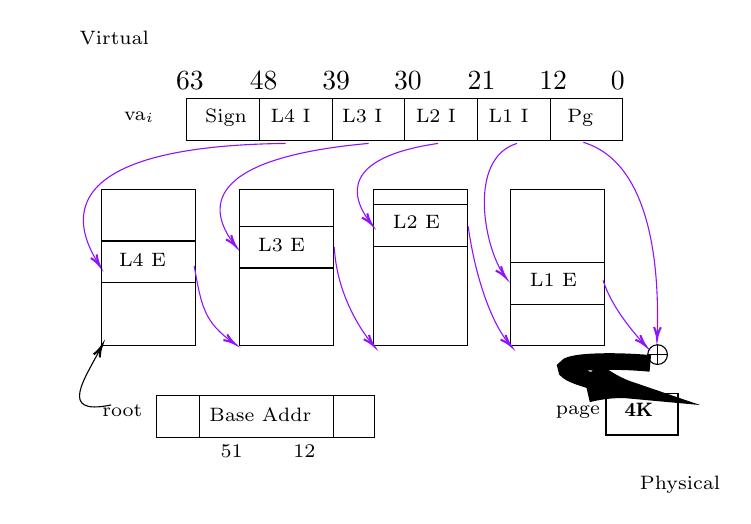
\begin{tikzpicture}[x=0.75pt,y=0.75pt,yscale=-0.5,xscale=0.5]
%uncomment if require: \path (0,476); %set diagram left start at 0, and has height of 476

%Shape: Rectangle [id:dp9406932326447903] 
\draw   (33,166) -- (123,166) -- (123,317) -- (33,317) -- cycle ;
%Shape: Rectangle [id:dp7682116051394419] 
\draw   (166,166) -- (256,166) -- (256,317) -- (166,317) -- cycle ;
%Shape: Rectangle [id:dp07376733516930423] 
\draw   (295,166) -- (385,166) -- (385,317) -- (295,317) -- cycle ;
%Shape: Rectangle [id:dp7106629147891306] 
\draw   (427,166) -- (517,166) -- (517,317) -- (427,317) -- cycle ;
%Shape: Rectangle [id:dp1342906826203598] 
\draw   (115,79) -- (185,79) -- (185,119) -- (115,119) -- cycle ;
%Shape: Rectangle [id:dp08072439007207399] 
\draw   (185,79) -- (255,79) -- (255,119) -- (185,119) -- cycle ;
%Shape: Rectangle [id:dp8282933603833216] 
\draw   (255,79) -- (325,79) -- (325,119) -- (255,119) -- cycle ;
%Shape: Rectangle [id:dp8416255090865326] 
\draw   (325,79) -- (395,79) -- (395,119) -- (325,119) -- cycle ;
%Shape: Rectangle [id:dp22911958218529804] 
\draw   (395,79) -- (465,79) -- (465,119) -- (395,119) -- cycle ;
%Shape: Rectangle [id:dp33732955213990756] 
\draw   (465,79) -- (535,79) -- (535,119) -- (465,119) -- cycle ;
%Curve Lines [id:da6688730321284677] 
\draw [color={rgb, 255:red, 144; green, 19; blue, 254 }  ,draw opacity=1 ]   (210,122) .. controls (-37.94,124.94) and (15.69,215.28) .. (30.17,238.65) ;
\draw [shift={(31,240)}, rotate = 238.24] [color={rgb, 255:red, 144; green, 19; blue, 254 }  ,draw opacity=1 ][line width=0.75]    (10.93,-3.29) .. controls (6.95,-1.4) and (3.31,-0.3) .. (0,0) .. controls (3.31,0.3) and (6.95,1.4) .. (10.93,3.29)   ;
%Shape: Rectangle [id:dp6044747978986409] 
\draw   (33,216) -- (123,216) -- (123,256) -- (33,256) -- cycle ;
%Curve Lines [id:da8867562998134584] 
\draw [color={rgb, 255:red, 144; green, 19; blue, 254 }  ,draw opacity=1 ]   (290,122) .. controls (116.54,137.68) and (140.92,193.7) .. (160.79,219.46) ;
\draw [shift={(162,221)}, rotate = 231.34] [color={rgb, 255:red, 144; green, 19; blue, 254 }  ,draw opacity=1 ][line width=0.75]    (10.93,-3.29) .. controls (6.95,-1.4) and (3.31,-0.3) .. (0,0) .. controls (3.31,0.3) and (6.95,1.4) .. (10.93,3.29)   ;
%Shape: Rectangle [id:dp8861153167245819] 
\draw   (166,202) -- (256,202) -- (256,242) -- (166,242) -- cycle ;
%Shape: Rectangle [id:dp05979844200848894] 
\draw   (295,181) -- (385,181) -- (385,221) -- (295,221) -- cycle ;
%Shape: Rectangle [id:dp17403733244247843] 
\draw   (427,237) -- (517,237) -- (517,277) -- (427,277) -- cycle ;
%Curve Lines [id:da20581124900573955] 
\draw [color={rgb, 255:red, 144; green, 19; blue, 254 }  ,draw opacity=1 ]   (357,122) .. controls (262.92,135.72) and (272.56,173.45) .. (291.81,198.48) ;
\draw [shift={(293,200)}, rotate = 231.34] [color={rgb, 255:red, 144; green, 19; blue, 254 }  ,draw opacity=1 ][line width=0.75]    (10.93,-3.29) .. controls (6.95,-1.4) and (3.31,-0.3) .. (0,0) .. controls (3.31,0.3) and (6.95,1.4) .. (10.93,3.29)   ;
%Curve Lines [id:da07589611603635316] 
\draw [color={rgb, 255:red, 144; green, 19; blue, 254 }  ,draw opacity=1 ]   (433,122) .. controls (384.98,136.7) and (401.31,222.47) .. (420.8,249.42) ;
\draw [shift={(422,251)}, rotate = 231.34] [color={rgb, 255:red, 144; green, 19; blue, 254 }  ,draw opacity=1 ][line width=0.75]    (10.93,-3.29) .. controls (6.95,-1.4) and (3.31,-0.3) .. (0,0) .. controls (3.31,0.3) and (6.95,1.4) .. (10.93,3.29)   ;
%Curve Lines [id:da017521077423665377] 
\draw    (42,374) .. controls (-10.21,384.84) and (17.15,348.13) .. (32.32,318.36) ;
\draw [shift={(33,317)}, rotate = 116.57] [color={rgb, 255:red, 0; green, 0; blue, 0 }  ][line width=0.75]    (10.93,-3.29) .. controls (6.95,-1.4) and (3.31,-0.3) .. (0,0) .. controls (3.31,0.3) and (6.95,1.4) .. (10.93,3.29)   ;
%Curve Lines [id:da6750042432035159] 
\draw [color={rgb, 255:red, 144; green, 19; blue, 254 }  ,draw opacity=1 ]   (122,240) .. controls (128.9,279.4) and (131.91,294.54) .. (159.71,314.1) ;
\draw [shift={(161,315)}, rotate = 214.59] [color={rgb, 255:red, 144; green, 19; blue, 254 }  ,draw opacity=1 ][line width=0.75]    (10.93,-3.29) .. controls (6.95,-1.4) and (3.31,-0.3) .. (0,0) .. controls (3.31,0.3) and (6.95,1.4) .. (10.93,3.29)   ;
%Curve Lines [id:da14788158682113428] 
\draw [color={rgb, 255:red, 144; green, 19; blue, 254 }  ,draw opacity=1 ]   (257,222) .. controls (258.95,261) and (277.06,295.25) .. (293.72,315.47) ;
\draw [shift={(295,317)}, rotate = 229.64] [color={rgb, 255:red, 144; green, 19; blue, 254 }  ,draw opacity=1 ][line width=0.75]    (10.93,-3.29) .. controls (6.95,-1.4) and (3.31,-0.3) .. (0,0) .. controls (3.31,0.3) and (6.95,1.4) .. (10.93,3.29)   ;
%Curve Lines [id:da3297977595767969] 
\draw [color={rgb, 255:red, 144; green, 19; blue, 254 }  ,draw opacity=1 ]   (386,202) .. controls (392.86,251) and (408.36,295.2) .. (425.92,315.77) ;
\draw [shift={(427,317)}, rotate = 228.01] [color={rgb, 255:red, 144; green, 19; blue, 254 }  ,draw opacity=1 ][line width=0.75]    (10.93,-3.29) .. controls (6.95,-1.4) and (3.31,-0.3) .. (0,0) .. controls (3.31,0.3) and (6.95,1.4) .. (10.93,3.29)   ;
%Shape: Rectangle [id:dp49428805993358815] 
\draw   (519,363) -- (589,363) -- (589,403) -- (519,403) -- cycle ;
%Shape: Rectangle [id:dp886191131490832] 
\draw   (86,365) -- (127.5,365) -- (127.5,405) -- (86,405) -- cycle ;
%Shape: Rectangle [id:dp7623210397795441] 
\draw   (127.5,365) -- (256.5,365) -- (256.5,405) -- (127.5,405) -- cycle ;
%Shape: Rectangle [id:dp41272095233228523] 
\draw   (256.5,365) -- (296,365) -- (296,405) -- (256.5,405) -- cycle ;
%Curve Lines [id:da25384974890834555] 
\draw [color={rgb, 255:red, 144; green, 19; blue, 254 }  ,draw opacity=1 ]   (497,121) .. controls (572.46,143.54) and (569.17,274.61) .. (568.06,308.07) ;
\draw [shift={(568,310)}, rotate = 271.91] [color={rgb, 255:red, 144; green, 19; blue, 254 }  ,draw opacity=1 ][line width=0.75]    (10.93,-3.29) .. controls (6.95,-1.4) and (3.31,-0.3) .. (0,0) .. controls (3.31,0.3) and (6.95,1.4) .. (10.93,3.29)   ;
%Curve Lines [id:da34682458787441517] 
\draw [color={rgb, 255:red, 144; green, 19; blue, 254 }  ,draw opacity=1 ]   (516,254) .. controls (523.76,278.25) and (542.81,301.56) .. (555.81,315.71) ;
\draw [shift={(557,317)}, rotate = 227.12] [color={rgb, 255:red, 144; green, 19; blue, 254 }  ,draw opacity=1 ][line width=0.75]    (10.93,-3.29) .. controls (6.95,-1.4) and (3.31,-0.3) .. (0,0) .. controls (3.31,0.3) and (6.95,1.4) .. (10.93,3.29)   ;
%Shape: Rectangle [id:dp9106415441109659] 
\draw   (518,363) -- (588,363) -- (588,403) -- (518,403) -- cycle ;
\draw   (559,325.5) .. controls (559,320.25) and (563.25,316) .. (568.5,316) .. controls (573.75,316) and (578,320.25) .. (578,325.5) .. controls (578,330.75) and (573.75,335) .. (568.5,335) .. controls (563.25,335) and (559,330.75) .. (559,325.5) -- cycle ; \draw   (559,325.5) -- (578,325.5) ; \draw   (568.5,316) -- (568.5,335) ;
%Curve Lines [id:da5209214352310081] 
\draw [color={rgb, 255:red, 0; green, 0; blue, 0 }  ,draw opacity=1 ][line width=6]    (561.5,334) .. controls (511.52,329.1) and (420.72,332.84) .. (536.17,358.41) ;
\draw [shift={(543.5,360)}, rotate = 192.05] [color={rgb, 255:red, 0; green, 0; blue, 0 }  ,draw opacity=1 ][line width=6]    (40.44,-12.17) .. controls (25.71,-5.16) and (12.23,-1.11) .. (0,0) .. controls (12.23,1.11) and (25.71,5.17) .. (40.44,12.17)   ;

% Text Node
\draw (9,11) node [anchor=north west][inner sep=0.75pt]   [align=left] {{\scriptsize Virtual}};
% Text Node
\draw (549,440) node [anchor=north west][inner sep=0.75pt]   [align=left] {{\scriptsize Physical}};
% Text Node
\draw (102,50) node [anchor=north west][inner sep=0.75pt]   [align=left] {63};
% Text Node
\draw (173,50) node [anchor=north west][inner sep=0.75pt]   [align=left] {48};
% Text Node
\draw (243,50) node [anchor=north west][inner sep=0.75pt]   [align=left] {39};
% Text Node
\draw (312,50) node [anchor=north west][inner sep=0.75pt]   [align=left] {30};
% Text Node
\draw (383,50) node [anchor=north west][inner sep=0.75pt]   [align=left] {21};
% Text Node
\draw (452,50) node [anchor=north west][inner sep=0.75pt]   [align=left] {12};
% Text Node
\draw (521,50) node [anchor=north west][inner sep=0.75pt]   [align=left] {0};
% Text Node
\draw (130,87) node [anchor=north west][inner sep=0.75pt]   [align=left] {{\scriptsize Sign}};
% Text Node
\draw (193,87) node [anchor=north west][inner sep=0.75pt]   [align=left] {{\scriptsize L4 I}};
% Text Node
\draw (262,87) node [anchor=north west][inner sep=0.75pt]   [align=left] {{\scriptsize L3 I}};
% Text Node
\draw (333,87) node [anchor=north west][inner sep=0.75pt]   [align=left] {{\scriptsize L2 I}};
% Text Node
\draw (403,87) node [anchor=north west][inner sep=0.75pt]   [align=left] {{\scriptsize L1 I}};
% Text Node
\draw (479,87) node [anchor=north west][inner sep=0.75pt]   [align=left] {{\scriptsize Pg}};
% Text Node
\draw (52,89) node [anchor=north west][inner sep=0.75pt]   [align=left] {{\scriptsize va$_i$}};
% Text Node
\draw (31,371) node [anchor=north west][inner sep=0.75pt]   [align=left] {{\scriptsize root}};
% Text Node
\draw (47,225) node [anchor=north west][inner sep=0.75pt]   [align=left] {{\scriptsize L4 E}};
% Text Node
\draw (181,211) node [anchor=north west][inner sep=0.75pt]   [align=left] {{\scriptsize L3 E}};
% Text Node
\draw (311,189) node [anchor=north west][inner sep=0.75pt]   [align=left] {{\scriptsize L2 E}};
% Text Node
\draw (443,245) node [anchor=north west][inner sep=0.75pt]   [align=left] {{\scriptsize L1 E}};
% Text Node
\draw (468,373) node [anchor=north west][inner sep=0.75pt]   [align=left] {{\scriptsize page}};
% Text Node
\draw (535,370) node [anchor=north west][inner sep=0.75pt]   [align=left] {{\scriptsize 4K}};
% Text Node
\draw (145,410) node [anchor=north west][inner sep=0.75pt]   [align=left] {{\scriptsize 51}};
% Text Node
\draw (215,410) node [anchor=north west][inner sep=0.75pt]   [align=left] {{\scriptsize 12}};
% Text Node
\draw (134,374) node [anchor=north west][inner sep=0.75pt]   [align=left] {{\scriptsize Base Addr}};
% Text Node
\draw (534,370) node [anchor=north west][inner sep=0.75pt]   [align=left] {{\scriptsize 4K}};


\end{tikzpicture}
       \caption{Sharing Page-Tables under Updates to Page-Tables}
        \label{fig:enter-label}
    \end{figure}
\end{frame}
\begin{frame}{Breaking Soundness in Sharing}
\begin{columns}[c]
    \column{0.65\textwidth}
    \begin{figure}
        \centering
\tikzset{every picture/.style={line width=0.75pt}} %set default line width to 0.75pt        
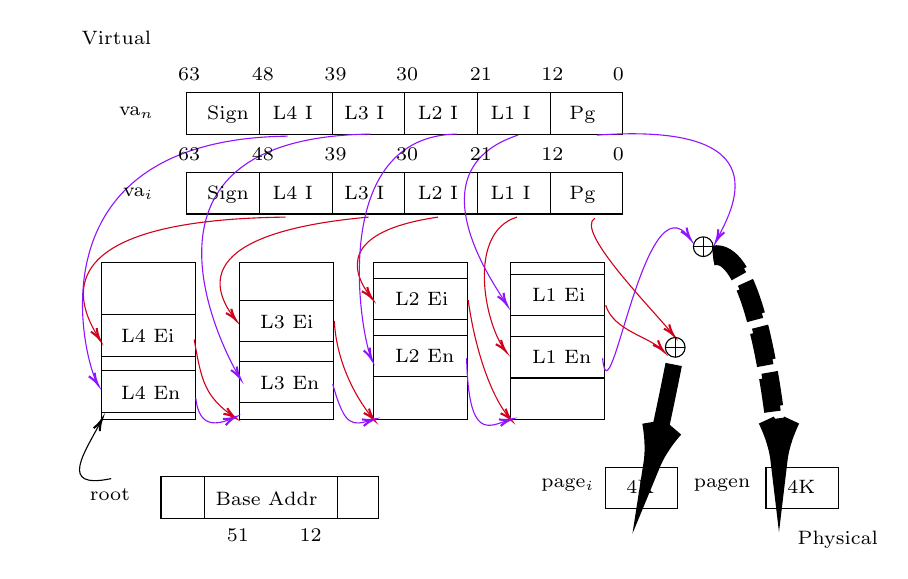
\begin{tikzpicture}[x=0.75pt,y=0.75pt,yscale=-0.5,xscale=0.5]
%uncomment if require: \path (0,532); %set diagram left start at 0, and has height of 532

%Shape: Rectangle [id:dp9406932326447903] 
\draw   (33,240) -- (123,240) -- (123,391) -- (33,391) -- cycle ;
%Shape: Rectangle [id:dp7682116051394419] 
\draw   (166,240) -- (256,240) -- (256,391) -- (166,391) -- cycle ;
%Shape: Rectangle [id:dp07376733516930423] 
\draw   (295,240) -- (385,240) -- (385,391) -- (295,391) -- cycle ;
%Shape: Rectangle [id:dp7106629147891306] 
\draw   (427,240) -- (517,240) -- (517,391) -- (427,391) -- cycle ;
%Shape: Rectangle [id:dp1342906826203598] 
\draw   (115,153) -- (185,153) -- (185,193) -- (115,193) -- cycle ;
%Shape: Rectangle [id:dp08072439007207399] 
\draw   (185,153) -- (255,153) -- (255,193) -- (185,193) -- cycle ;
%Shape: Rectangle [id:dp8282933603833216] 
\draw   (255,153) -- (325,153) -- (325,193) -- (255,193) -- cycle ;
%Shape: Rectangle [id:dp8416255090865326] 
\draw   (325,153) -- (395,153) -- (395,193) -- (325,193) -- cycle ;
%Shape: Rectangle [id:dp22911958218529804] 
\draw   (395,153) -- (465,153) -- (465,193) -- (395,193) -- cycle ;
%Shape: Rectangle [id:dp33732955213990756] 
\draw   (465,153) -- (535,153) -- (535,193) -- (465,193) -- cycle ;
%Shape: Rectangle [id:dp6628879501744147] 
\draw   (518,437) -- (588,437) -- (588,477) -- (518,477) -- cycle ;
%Curve Lines [id:da6688730321284677] 
\draw [color={rgb, 255:red, 208; green, 2; blue, 27 }  ,draw opacity=1 ]   (210,196) .. controls (-37.94,198.94) and (15.69,289.28) .. (30.17,312.65) ;
\draw [shift={(31,314)}, rotate = 238.24] [color={rgb, 255:red, 208; green, 2; blue, 27 }  ,draw opacity=1 ][line width=0.75]    (10.93,-3.29) .. controls (6.95,-1.4) and (3.31,-0.3) .. (0,0) .. controls (3.31,0.3) and (6.95,1.4) .. (10.93,3.29)   ;
%Shape: Rectangle [id:dp6044747978986409] 
\draw   (33,290) -- (123,290) -- (123,330) -- (33,330) -- cycle ;
%Curve Lines [id:da8867562998134584] 
\draw [color={rgb, 255:red, 208; green, 2; blue, 27 }  ,draw opacity=1 ]   (290,196) .. controls (116.54,211.68) and (140.92,267.7) .. (160.79,293.46) ;
\draw [shift={(162,295)}, rotate = 231.34] [color={rgb, 255:red, 208; green, 2; blue, 27 }  ,draw opacity=1 ][line width=0.75]    (10.93,-3.29) .. controls (6.95,-1.4) and (3.31,-0.3) .. (0,0) .. controls (3.31,0.3) and (6.95,1.4) .. (10.93,3.29)   ;
%Shape: Rectangle [id:dp8861153167245819] 
\draw   (166,276) -- (256,276) -- (256,316) -- (166,316) -- cycle ;
%Shape: Rectangle [id:dp05979844200848894] 
\draw   (295,255) -- (385,255) -- (385,295) -- (295,295) -- cycle ;
%Shape: Rectangle [id:dp17403733244247843] 
\draw   (427,311) -- (517,311) -- (517,351) -- (427,351) -- cycle ;
%Curve Lines [id:da20581124900573955] 
\draw [color={rgb, 255:red, 208; green, 2; blue, 27 }  ,draw opacity=1 ]   (357,196) .. controls (262.92,209.72) and (272.56,247.45) .. (291.81,272.48) ;
\draw [shift={(293,274)}, rotate = 231.34] [color={rgb, 255:red, 208; green, 2; blue, 27 }  ,draw opacity=1 ][line width=0.75]    (10.93,-3.29) .. controls (6.95,-1.4) and (3.31,-0.3) .. (0,0) .. controls (3.31,0.3) and (6.95,1.4) .. (10.93,3.29)   ;
%Curve Lines [id:da07589611603635316] 
\draw [color={rgb, 255:red, 208; green, 2; blue, 27 }  ,draw opacity=1 ]   (433,196) .. controls (384.98,210.7) and (401.31,296.47) .. (420.8,323.42) ;
\draw [shift={(422,325)}, rotate = 231.34] [color={rgb, 255:red, 208; green, 2; blue, 27 }  ,draw opacity=1 ][line width=0.75]    (10.93,-3.29) .. controls (6.95,-1.4) and (3.31,-0.3) .. (0,0) .. controls (3.31,0.3) and (6.95,1.4) .. (10.93,3.29)   ;
%Curve Lines [id:da6852167546673456] 
\draw [color={rgb, 255:red, 208; green, 2; blue, 27 }  ,draw opacity=1 ]   (508,197) .. controls (488.3,208.82) and (561.74,282.73) .. (583.06,308.84) ;
\draw [shift={(584,310)}, rotate = 231.34] [color={rgb, 255:red, 208; green, 2; blue, 27 }  ,draw opacity=1 ][line width=0.75]    (10.93,-3.29) .. controls (6.95,-1.4) and (3.31,-0.3) .. (0,0) .. controls (3.31,0.3) and (6.95,1.4) .. (10.93,3.29)   ;
%Curve Lines [id:da6285305490382367] 
\draw [color={rgb, 255:red, 0; green, 0; blue, 0 }  ,draw opacity=1 ][line width=6]    (584,338) .. controls (581.75,349.7) and (571.81,399.47) .. (564.74,427.53) ;
\draw [shift={(562.5,436)}, rotate = 285.64] [color={rgb, 255:red, 0; green, 0; blue, 0 }  ,draw opacity=1 ][line width=6]    (40.44,-12.17) .. controls (25.71,-5.16) and (12.23,-1.11) .. (0,0) .. controls (12.23,1.11) and (25.71,5.17) .. (40.44,12.17)   ;
%Curve Lines [id:da017521077423665377] 
\draw    (42,448) .. controls (-10.21,458.84) and (17.15,422.13) .. (32.32,392.36) ;
\draw [shift={(33,391)}, rotate = 116.57] [color={rgb, 255:red, 0; green, 0; blue, 0 }  ][line width=0.75]    (10.93,-3.29) .. controls (6.95,-1.4) and (3.31,-0.3) .. (0,0) .. controls (3.31,0.3) and (6.95,1.4) .. (10.93,3.29)   ;
%Curve Lines [id:da6750042432035159] 
\draw [color={rgb, 255:red, 208; green, 2; blue, 27 }  ,draw opacity=1 ]   (122,314) .. controls (128.9,353.4) and (131.91,368.54) .. (159.71,388.1) ;
\draw [shift={(161,389)}, rotate = 214.59] [color={rgb, 255:red, 208; green, 2; blue, 27 }  ,draw opacity=1 ][line width=0.75]    (10.93,-3.29) .. controls (6.95,-1.4) and (3.31,-0.3) .. (0,0) .. controls (3.31,0.3) and (6.95,1.4) .. (10.93,3.29)   ;
%Curve Lines [id:da14788158682113428] 
\draw [color={rgb, 255:red, 208; green, 2; blue, 27 }  ,draw opacity=1 ]   (257,296) .. controls (258.95,335) and (277.06,369.25) .. (293.72,389.47) ;
\draw [shift={(295,391)}, rotate = 229.64] [color={rgb, 255:red, 208; green, 2; blue, 27 }  ,draw opacity=1 ][line width=0.75]    (10.93,-3.29) .. controls (6.95,-1.4) and (3.31,-0.3) .. (0,0) .. controls (3.31,0.3) and (6.95,1.4) .. (10.93,3.29)   ;
%Curve Lines [id:da3297977595767969] 
\draw [color={rgb, 255:red, 208; green, 2; blue, 27 }  ,draw opacity=1 ]   (386,276) .. controls (392.86,325) and (408.36,369.2) .. (425.92,389.77) ;
\draw [shift={(427,391)}, rotate = 228.01] [color={rgb, 255:red, 208; green, 2; blue, 27 }  ,draw opacity=1 ][line width=0.75]    (10.93,-3.29) .. controls (6.95,-1.4) and (3.31,-0.3) .. (0,0) .. controls (3.31,0.3) and (6.95,1.4) .. (10.93,3.29)   ;
%Curve Lines [id:da7710391961792686] 
\draw [color={rgb, 255:red, 208; green, 2; blue, 27 }  ,draw opacity=1 ]   (518.5,281) .. controls (526.26,305.25) and (558.95,310.68) .. (572.77,323.76) ;
\draw [shift={(574,325)}, rotate = 227.12] [color={rgb, 255:red, 208; green, 2; blue, 27 }  ,draw opacity=1 ][line width=0.75]    (10.93,-3.29) .. controls (6.95,-1.4) and (3.31,-0.3) .. (0,0) .. controls (3.31,0.3) and (6.95,1.4) .. (10.93,3.29)   ;
%Shape: Rectangle [id:dp8163096906532217] 
\draw   (115,76) -- (185,76) -- (185,116) -- (115,116) -- cycle ;
%Shape: Rectangle [id:dp5008947189169124] 
\draw   (185,76) -- (255,76) -- (255,116) -- (185,116) -- cycle ;
%Shape: Rectangle [id:dp20199565750745574] 
\draw   (255,76) -- (325,76) -- (325,116) -- (255,116) -- cycle ;
%Shape: Rectangle [id:dp6456722127145564] 
\draw   (325,76) -- (395,76) -- (395,116) -- (325,116) -- cycle ;
%Shape: Rectangle [id:dp2840441308370316] 
\draw   (395,76) -- (465,76) -- (465,116) -- (395,116) -- cycle ;
%Shape: Rectangle [id:dp8377187529278063] 
\draw   (465,76) -- (535,76) -- (535,116) -- (465,116) -- cycle ;
%Shape: Rectangle [id:dp8211934221770631] 
\draw   (33,344) -- (123,344) -- (123,384) -- (33,384) -- cycle ;
%Shape: Rectangle [id:dp8913167857456976] 
\draw   (166,335) -- (256,335) -- (256,375) -- (166,375) -- cycle ;
%Shape: Rectangle [id:dp9695091175432768] 
\draw   (295,310) -- (385,310) -- (385,350) -- (295,350) -- cycle ;
%Shape: Rectangle [id:dp6695852511595983] 
\draw   (427,251) -- (517,251) -- (517,291) -- (427,291) -- cycle ;
%Shape: Rectangle [id:dp7443372414988962] 
\draw   (673,437) -- (743,437) -- (743,477) -- (673,477) -- cycle ;
%Curve Lines [id:da8585420033251991] 
\draw [color={rgb, 255:red, 144; green, 19; blue, 254 }  ,draw opacity=1 ]   (212,118) .. controls (-35.94,120.94) and (13.84,327.48) .. (28.17,355.51) ;
\draw [shift={(29,357)}, rotate = 238.24] [color={rgb, 255:red, 144; green, 19; blue, 254 }  ,draw opacity=1 ][line width=0.75]    (10.93,-3.29) .. controls (6.95,-1.4) and (3.31,-0.3) .. (0,0) .. controls (3.31,0.3) and (6.95,1.4) .. (10.93,3.29)   ;
%Curve Lines [id:da3950862908580315] 
\draw [color={rgb, 255:red, 144; green, 19; blue, 254 }  ,draw opacity=1 ]   (292,116) .. controls (44.06,118.94) and (148.59,321.64) .. (165.1,349.52) ;
\draw [shift={(166,351)}, rotate = 238.24] [color={rgb, 255:red, 144; green, 19; blue, 254 }  ,draw opacity=1 ][line width=0.75]    (10.93,-3.29) .. controls (6.95,-1.4) and (3.31,-0.3) .. (0,0) .. controls (3.31,0.3) and (6.95,1.4) .. (10.93,3.29)   ;
%Curve Lines [id:da33073679964999325] 
\draw [color={rgb, 255:red, 144; green, 19; blue, 254 }  ,draw opacity=1 ]   (375,116) .. controls (252.5,117.96) and (280.78,302.4) .. (292.32,331.42) ;
\draw [shift={(293,333)}, rotate = 244.44] [color={rgb, 255:red, 144; green, 19; blue, 254 }  ,draw opacity=1 ][line width=0.75]    (10.93,-3.29) .. controls (6.95,-1.4) and (3.31,-0.3) .. (0,0) .. controls (3.31,0.3) and (6.95,1.4) .. (10.93,3.29)   ;
%Curve Lines [id:da8024795963071514] 
\draw [color={rgb, 255:red, 144; green, 19; blue, 254 }  ,draw opacity=1 ]   (434,117) .. controls (333.57,150.15) and (408.07,256.5) .. (422.05,278.48) ;
\draw [shift={(423,280)}, rotate = 238.57] [color={rgb, 255:red, 144; green, 19; blue, 254 }  ,draw opacity=1 ][line width=0.75]    (10.93,-3.29) .. controls (6.95,-1.4) and (3.31,-0.3) .. (0,0) .. controls (3.31,0.3) and (6.95,1.4) .. (10.93,3.29)   ;
%Curve Lines [id:da02032635448677178] 
\draw [color={rgb, 255:red, 144; green, 19; blue, 254 }  ,draw opacity=1 ]   (510,117) .. controls (690.32,104.26) and (640.14,189.48) .. (625.83,217.37) ;
\draw [shift={(625,219)}, rotate = 296.57] [color={rgb, 255:red, 144; green, 19; blue, 254 }  ,draw opacity=1 ][line width=0.75]    (10.93,-3.29) .. controls (6.95,-1.4) and (3.31,-0.3) .. (0,0) .. controls (3.31,0.3) and (6.95,1.4) .. (10.93,3.29)   ;
%Curve Lines [id:da41060712415524825] 
\draw [color={rgb, 255:red, 0; green, 0; blue, 0 }  ,draw opacity=1 ][line width=6]  [dash pattern={on 12.38pt off 4.5pt}]  (621.68,231.53) .. controls (622.92,231.26) and (624.14,231.13) .. (625.34,231.13) .. controls (633.77,231.13) and (641.39,237.71) .. (648.05,248.98) .. controls (659.27,267.99) and (667.85,300.17) .. (674.03,332.37) .. controls (681.19,369.64) and (685.18,406.91) .. (686,417.65)(622.32,234.47) .. controls (623.34,234.24) and (624.35,234.13) .. (625.34,234.13) .. controls (632.96,234.13) and (639.57,240.52) .. (645.47,250.5) .. controls (656.56,269.29) and (664.97,301.12) .. (671.09,332.94) .. controls (678.22,370.07) and (682.2,407.21) .. (683.01,417.91) ;
\draw [shift={(685.5,432)}, rotate = 270] [color={rgb, 255:red, 0; green, 0; blue, 0 }  ,draw opacity=1 ][line width=6]    (40.44,-12.17) .. controls (25.71,-5.16) and (12.23,-1.11) .. (0,0) .. controls (12.23,1.11) and (25.71,5.17) .. (40.44,12.17)   ;
%Curve Lines [id:da15754024469049188] 
\draw [color={rgb, 255:red, 144; green, 19; blue, 254 }  ,draw opacity=1 ]   (123.5,370) .. controls (126.4,399.92) and (144.19,396.31) .. (159.36,389.73) ;
\draw [shift={(161,389)}, rotate = 155.7] [color={rgb, 255:red, 144; green, 19; blue, 254 }  ,draw opacity=1 ][line width=0.75]    (10.93,-3.29) .. controls (6.95,-1.4) and (3.31,-0.3) .. (0,0) .. controls (3.31,0.3) and (6.95,1.4) .. (10.93,3.29)   ;
%Curve Lines [id:da2801023256877153] 
\draw [color={rgb, 255:red, 144; green, 19; blue, 254 }  ,draw opacity=1 ]   (255.5,357) .. controls (267.14,398.71) and (274.08,397.14) .. (293.19,391.53) ;
\draw [shift={(295,391)}, rotate = 163.69] [color={rgb, 255:red, 144; green, 19; blue, 254 }  ,draw opacity=1 ][line width=0.75]    (10.93,-3.29) .. controls (6.95,-1.4) and (3.31,-0.3) .. (0,0) .. controls (3.31,0.3) and (6.95,1.4) .. (10.93,3.29)   ;
%Curve Lines [id:da5373695051918006] 
\draw [color={rgb, 255:red, 144; green, 19; blue, 254 }  ,draw opacity=1 ]   (384.5,332) .. controls (386.44,411.54) and (405.32,397.93) .. (425.16,391.57) ;
\draw [shift={(427,391)}, rotate = 163.69] [color={rgb, 255:red, 144; green, 19; blue, 254 }  ,draw opacity=1 ][line width=0.75]    (10.93,-3.29) .. controls (6.95,-1.4) and (3.31,-0.3) .. (0,0) .. controls (3.31,0.3) and (6.95,1.4) .. (10.93,3.29)   ;
%Curve Lines [id:da8840761934459798] 
\draw [color={rgb, 255:red, 144; green, 19; blue, 254 }  ,draw opacity=1 ]   (515.5,332) .. controls (522.47,399.66) and (555.67,155.46) .. (599.34,216.06) ;
\draw [shift={(600,217)}, rotate = 235.49] [color={rgb, 255:red, 144; green, 19; blue, 254 }  ,draw opacity=1 ][line width=0.75]    (10.93,-3.29) .. controls (6.95,-1.4) and (3.31,-0.3) .. (0,0) .. controls (3.31,0.3) and (6.95,1.4) .. (10.93,3.29)   ;
%Shape: Rectangle [id:dp967281283756027] 
\draw   (90,446) -- (131.5,446) -- (131.5,486) -- (90,486) -- cycle ;
%Shape: Rectangle [id:dp6818362650206453] 
\draw   (131.5,446) -- (260.5,446) -- (260.5,486) -- (131.5,486) -- cycle ;
%Shape: Rectangle [id:dp6367652388585874] 
\draw   (260.5,446) -- (300,446) -- (300,486) -- (260.5,486) -- cycle ;
\draw   (576,321.5) .. controls (576,316.25) and (580.25,312) .. (585.5,312) .. controls (590.75,312) and (595,316.25) .. (595,321.5) .. controls (595,326.75) and (590.75,331) .. (585.5,331) .. controls (580.25,331) and (576,326.75) .. (576,321.5) -- cycle ; \draw   (576,321.5) -- (595,321.5) ; \draw   (585.5,312) -- (585.5,331) ;
\draw   (603,224.5) .. controls (603,219.25) and (607.25,215) .. (612.5,215) .. controls (617.75,215) and (622,219.25) .. (622,224.5) .. controls (622,229.75) and (617.75,234) .. (612.5,234) .. controls (607.25,234) and (603,229.75) .. (603,224.5) -- cycle ; \draw   (603,224.5) -- (622,224.5) ; \draw   (612.5,215) -- (612.5,234) ;

% Text Node
\draw (11,14) node [anchor=north west][inner sep=0.75pt]   [align=left] {{\scriptsize Virtual}};
% Text Node
\draw (701,496) node [anchor=north west][inner sep=0.75pt]   [align=left] {{\scriptsize Physical}};
% Text Node
\draw (104,127) node [anchor=north west][inner sep=0.75pt]   [align=left] {{\scriptsize 63}};
% Text Node
\draw (175,127) node [anchor=north west][inner sep=0.75pt]   [align=left] {{\scriptsize 48}};
% Text Node
\draw (245,127) node [anchor=north west][inner sep=0.75pt]   [align=left] {{\scriptsize 39}};
% Text Node
\draw (314,127) node [anchor=north west][inner sep=0.75pt]   [align=left] {{\scriptsize 30}};
% Text Node
\draw (385,127) node [anchor=north west][inner sep=0.75pt]   [align=left] {{\scriptsize 21}};
% Text Node
\draw (454,127) node [anchor=north west][inner sep=0.75pt]   [align=left] {{\scriptsize 12}};
% Text Node
\draw (523,127) node [anchor=north west][inner sep=0.75pt]   [align=left] {{\scriptsize 0}};
% Text Node
\draw (132,164) node [anchor=north west][inner sep=0.75pt]   [align=left] {{\scriptsize Sign}};
% Text Node
\draw (195,164) node [anchor=north west][inner sep=0.75pt]   [align=left] {{\scriptsize L4 I}};
% Text Node
\draw (264,164) node [anchor=north west][inner sep=0.75pt]   [align=left] {{\scriptsize L3 I}};
% Text Node
\draw (335,164) node [anchor=north west][inner sep=0.75pt]   [align=left] {{\scriptsize L2 I}};
% Text Node
\draw (405,164) node [anchor=north west][inner sep=0.75pt]   [align=left] {{\scriptsize L1 I}};
% Text Node
\draw (481,164) node [anchor=north west][inner sep=0.75pt]   [align=left] {{\scriptsize Pg}};
% Text Node
\draw (51,166) node [anchor=north west][inner sep=0.75pt]   [align=left] {{\scriptsize va$_i$}};
% Text Node
\draw (19,455) node [anchor=north west][inner sep=0.75pt]   [align=left] {{\scriptsize root}};
% Text Node
\draw (454,446) node [anchor=north west][inner sep=0.75pt]   [align=left] {{\scriptsize page$_i$}};
% Text Node
\draw (536,447) node [anchor=north west][inner sep=0.75pt]   [align=left] {{\scriptsize 4K}};
% Text Node
\draw (49,302) node [anchor=north west][inner sep=0.75pt]   [align=left] {{\scriptsize L4 Ei}};
% Text Node
\draw (183,288) node [anchor=north west][inner sep=0.75pt]   [align=left] {{\scriptsize L3 Ei}};
% Text Node
\draw (313,266) node [anchor=north west][inner sep=0.75pt]   [align=left] {{\scriptsize L2 Ei}};
% Text Node
\draw (445,322) node [anchor=north west][inner sep=0.75pt]   [align=left] {{\scriptsize L1 En}};
% Text Node
\draw (104,50) node [anchor=north west][inner sep=0.75pt]   [align=left] {{\scriptsize 63}};
% Text Node
\draw (175,50) node [anchor=north west][inner sep=0.75pt]   [align=left] {{\scriptsize 48}};
% Text Node
\draw (245,50) node [anchor=north west][inner sep=0.75pt]   [align=left] {{\scriptsize 39}};
% Text Node
\draw (314,50) node [anchor=north west][inner sep=0.75pt]   [align=left] {{\scriptsize 30}};
% Text Node
\draw (385,50) node [anchor=north west][inner sep=0.75pt]   [align=left] {{\scriptsize 21}};
% Text Node
\draw (454,50) node [anchor=north west][inner sep=0.75pt]   [align=left] {{\scriptsize 12}};
% Text Node
\draw (523,50) node [anchor=north west][inner sep=0.75pt]   [align=left] {{\scriptsize 0}};
% Text Node
\draw (132,87) node [anchor=north west][inner sep=0.75pt]   [align=left] {{\scriptsize Sign}};
% Text Node
\draw (195,87) node [anchor=north west][inner sep=0.75pt]   [align=left] {{\scriptsize L4 I}};
% Text Node
\draw (264,87) node [anchor=north west][inner sep=0.75pt]   [align=left] {{\scriptsize L3 I}};
% Text Node
\draw (335,87) node [anchor=north west][inner sep=0.75pt]   [align=left] {{\scriptsize L2 I}};
% Text Node
\draw (405,87) node [anchor=north west][inner sep=0.75pt]   [align=left] {{\scriptsize L1 I}};
% Text Node
\draw (481,87) node [anchor=north west][inner sep=0.75pt]   [align=left] {{\scriptsize Pg}};
% Text Node
\draw (47,88) node [anchor=north west][inner sep=0.75pt]   [align=left] {{\scriptsize va$_n$}};
% Text Node
\draw (49,356) node [anchor=north west][inner sep=0.75pt]   [align=left] {{\scriptsize L4 En}};
% Text Node
\draw (183,347) node [anchor=north west][inner sep=0.75pt]   [align=left] {{\scriptsize L3 En}};
% Text Node
\draw (313,321) node [anchor=north west][inner sep=0.75pt]   [align=left] {{\scriptsize L2 En}};
% Text Node
\draw (445,262) node [anchor=north west][inner sep=0.75pt]   [align=left] {{\scriptsize L1 Ei}};
% Text Node
\draw (601,446) node [anchor=north west][inner sep=0.75pt]   [align=left] {{\scriptsize pagen}};
% Text Node
\draw (691,447) node [anchor=north west][inner sep=0.75pt]   [align=left] {{\scriptsize 4K}};
% Text Node
\draw (151,494) node [anchor=north west][inner sep=0.75pt]   [align=left] {{\scriptsize 51}};
% Text Node
\draw (221,494) node [anchor=north west][inner sep=0.75pt]   [align=left] {{\scriptsize 12}};
% Text Node
\draw (140,458) node [anchor=north west][inner sep=0.75pt]   [align=left] {{\scriptsize Base Addr}};


\end{tikzpicture}
     %  \caption{Bs}
      %  \label{fig:enter-label}
    \end{figure}
    \column{0.30\textwidth}
    \begin{alertblock}{Soundness of Traversal}
    Any update on the \emph{shared page-tables}, which themselves are referenced with \emph{physical memory} addresses, would break the soundness of any other traversal!
    \end{alertblock}
    \end{columns}
\end{frame}
\subsection{Address-Space Agnostic Virtual Memory References}
\begin{frame}{Managing Agnostic Memory Mappings}
    \begin{figure}
        \centering




\tikzset{every picture/.style={line width=0.75pt}} %set default line width to 0.75pt        

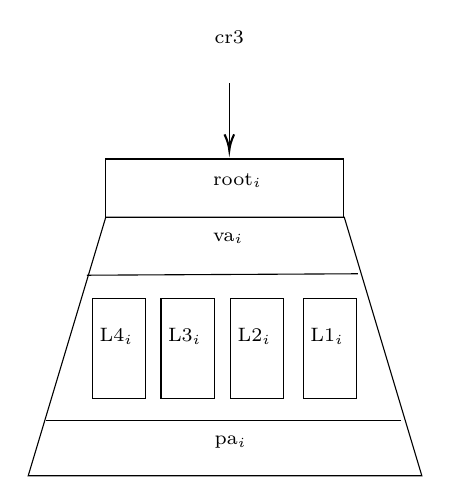
\begin{tikzpicture}[x=0.75pt,y=0.75pt,yscale=-0.7,xscale=0.7]
%uncomment if require: \path (0,444); %set diagram left start at 0, and has height of 444

%Straight Lines [id:da6068809865252034] 
\draw    (179,78) -- (179,122) ;
\draw [shift={(179,124)}, rotate = 270] [color={rgb, 255:red, 0; green, 0; blue, 0 }  ][line width=0.75]    (10.93,-3.29) .. controls (6.95,-1.4) and (3.31,-0.3) .. (0,0) .. controls (3.31,0.3) and (6.95,1.4) .. (10.93,3.29)   ;
%Shape: Trapezoid [id:dp3739735856439024] 
\draw   (40.6,348) -- (94,170) -- (258.1,170) -- (311.5,348) -- cycle ;
%Shape: Rectangle [id:dp6026336395414527] 
\draw   (94,130) -- (257.5,130) -- (257.5,170) -- (94,170) -- cycle ;
%Straight Lines [id:da32976073844810716] 
\draw    (81,210) -- (267.5,209) ;
%Straight Lines [id:da4667182831758503] 
\draw    (53,310) -- (297.5,310) ;
%Shape: Rectangle [id:dp3480638833922085] 
\draw   (85,226) -- (121.5,226) -- (121.5,295) -- (85,295) -- cycle ;
%Shape: Rectangle [id:dp558691590623291] 
\draw   (132,226) -- (168.5,226) -- (168.5,295) -- (132,295) -- cycle ;
%Shape: Rectangle [id:dp5224364674753033] 
\draw   (180,226) -- (216.5,226) -- (216.5,295) -- (180,295) -- cycle ;
%Shape: Rectangle [id:dp7593362242110164] 
\draw   (230,226) -- (266.5,226) -- (266.5,295) -- (230,295) -- cycle ;

% Text Node
\draw (167,40) node [anchor=north west][inner sep=0.75pt]   [align=left] {{\scriptsize cr3}};
% Text Node
\draw (166,179) node [anchor=north west][inner sep=0.75pt]   [align=left] {{\scriptsize va$_i$}};
% Text Node
\draw (167,319) node [anchor=north west][inner sep=0.75pt]   [align=left] {{\scriptsize pa$_i$}};
% Text Node
\draw (88,245) node [anchor=north west][inner sep=0.75pt]   [align=left] {{\scriptsize L4$_i$}};
% Text Node
\draw (166,138) node [anchor=north west][inner sep=0.75pt]   [align=left] {{\scriptsize root$_i$}};
% Text Node
\draw (135,245) node [anchor=north west][inner sep=0.75pt]   [align=left] {{\scriptsize L3$_i$}};
% Text Node
\draw (183,245) node [anchor=north west][inner sep=0.75pt]   [align=left] {{\scriptsize L2$_i$}};
% Text Node
\draw (233,245) node [anchor=north west][inner sep=0.75pt]   [align=left] {{\scriptsize L1$_i$}};


\end{tikzpicture}
        \caption{An Address Space with Unique Root Address \textsf{root}$_i$}
        \label{fig:enter-label}
    \end{figure}
\end{frame}
\begin{frame}{Managing Agnostic Memory Mappings}
    \begin{figure}
        \centering
        


\tikzset{every picture/.style={line width=0.75pt}} %set default line width to 0.75pt        

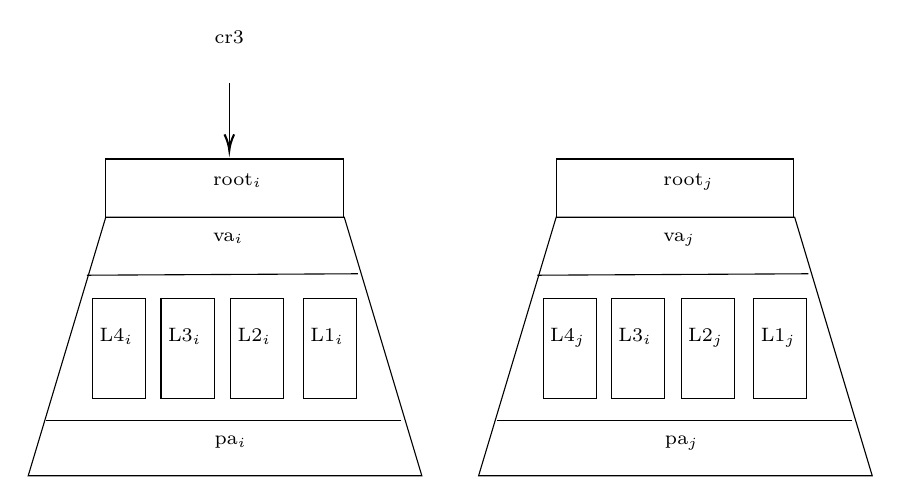
\begin{tikzpicture}[x=0.75pt,y=0.75pt,yscale=-0.7,xscale=0.7]
%uncomment if require: \path (0,444); %set diagram left start at 0, and has height of 444

%Straight Lines [id:da6068809865252034] 
\draw    (179,78) -- (179,122) ;
\draw [shift={(179,124)}, rotate = 270] [color={rgb, 255:red, 0; green, 0; blue, 0 }  ][line width=0.75]    (10.93,-3.29) .. controls (6.95,-1.4) and (3.31,-0.3) .. (0,0) .. controls (3.31,0.3) and (6.95,1.4) .. (10.93,3.29)   ;
%Shape: Trapezoid [id:dp3739735856439024] 
\draw   (40.6,348) -- (94,170) -- (258.1,170) -- (311.5,348) -- cycle ;
%Shape: Rectangle [id:dp6026336395414527] 
\draw   (94,130) -- (257.5,130) -- (257.5,170) -- (94,170) -- cycle ;
%Straight Lines [id:da32976073844810716] 
\draw    (81,210) -- (267.5,209) ;
%Straight Lines [id:da4667182831758503] 
\draw    (53,310) -- (297.5,310) ;
%Shape: Rectangle [id:dp3480638833922085] 
\draw   (85,226) -- (121.5,226) -- (121.5,295) -- (85,295) -- cycle ;
%Shape: Rectangle [id:dp558691590623291] 
\draw   (132,226) -- (168.5,226) -- (168.5,295) -- (132,295) -- cycle ;
%Shape: Rectangle [id:dp5224364674753033] 
\draw   (180,226) -- (216.5,226) -- (216.5,295) -- (180,295) -- cycle ;
%Shape: Rectangle [id:dp7593362242110164] 
\draw   (230,226) -- (266.5,226) -- (266.5,295) -- (230,295) -- cycle ;
%Shape: Trapezoid [id:dp17680532195155196] 
\draw   (350.6,348) -- (404,170) -- (568.1,170) -- (621.5,348) -- cycle ;
%Shape: Rectangle [id:dp1391273388270049] 
\draw   (404,130) -- (567.5,130) -- (567.5,170) -- (404,170) -- cycle ;
%Straight Lines [id:da16412176418294644] 
\draw    (391,210) -- (577.5,209) ;
%Straight Lines [id:da02392113930828521] 
\draw    (363,310) -- (607.5,310) ;
%Shape: Rectangle [id:dp3343779414527479] 
\draw   (395,226) -- (431.5,226) -- (431.5,295) -- (395,295) -- cycle ;
%Shape: Rectangle [id:dp5031533033051587] 
\draw   (442,226) -- (478.5,226) -- (478.5,295) -- (442,295) -- cycle ;
%Shape: Rectangle [id:dp6176432721746983] 
\draw   (490,226) -- (526.5,226) -- (526.5,295) -- (490,295) -- cycle ;
%Shape: Rectangle [id:dp8967436529993302] 
\draw   (540,226) -- (576.5,226) -- (576.5,295) -- (540,295) -- cycle ;

% Text Node
\draw (167,40) node [anchor=north west][inner sep=0.75pt]   [align=left] {{\scriptsize cr3}};
% Text Node
\draw (166,179) node [anchor=north west][inner sep=0.75pt]   [align=left] {{\scriptsize va$_i$}};
% Text Node
\draw (167,319) node [anchor=north west][inner sep=0.75pt]   [align=left] {{\scriptsize pa$_i$}};
% Text Node
\draw (88,245) node [anchor=north west][inner sep=0.75pt]   [align=left] {{\scriptsize L4$_i$}};
% Text Node
\draw (166,138) node [anchor=north west][inner sep=0.75pt]   [align=left] {{\scriptsize root$_i$}};
% Text Node
\draw (135,245) node [anchor=north west][inner sep=0.75pt]   [align=left] {{\scriptsize L3$_i$}};
% Text Node
\draw (183,245) node [anchor=north west][inner sep=0.75pt]   [align=left] {{\scriptsize L2$_i$}};
% Text Node
\draw (233,245) node [anchor=north west][inner sep=0.75pt]   [align=left] {{\scriptsize L1$_i$}};
% Text Node
\draw (476,179) node [anchor=north west][inner sep=0.75pt]   [align=left] {{\scriptsize va$_j$}};
% Text Node
\draw (477,319) node [anchor=north west][inner sep=0.75pt]   [align=left] {{\scriptsize pa$_j$}};
% Text Node
\draw (398,245) node [anchor=north west][inner sep=0.75pt]   [align=left] {{\scriptsize L4$_j$}};
% Text Node
\draw (476,138) node [anchor=north west][inner sep=0.75pt]   [align=left] {{\scriptsize root$_j$}};
% Text Node
\draw (445,245) node [anchor=north west][inner sep=0.75pt]   [align=left] {{\scriptsize L3$_i$}};
% Text Node
\draw (493,245) node [anchor=north west][inner sep=0.75pt]   [align=left] {{\scriptsize L2$_j$}};
% Text Node
\draw (543,245) node [anchor=north west][inner sep=0.75pt]   [align=left] {{\scriptsize L1$_j$}};


\end{tikzpicture}
        \caption{Two Address-Spaces with the Unique Root Addresses \textsf{root}$_i$ and \textsf{root}$_j$}
        \label{fig:enter-label}
    \end{figure}
   
\end{frame}
\begin{frame}{Managing Agnostic Memory Mappings}
    \begin{figure}
        \centering
        


\tikzset{every picture/.style={line width=0.75pt}} %set default line width to 0.75pt        

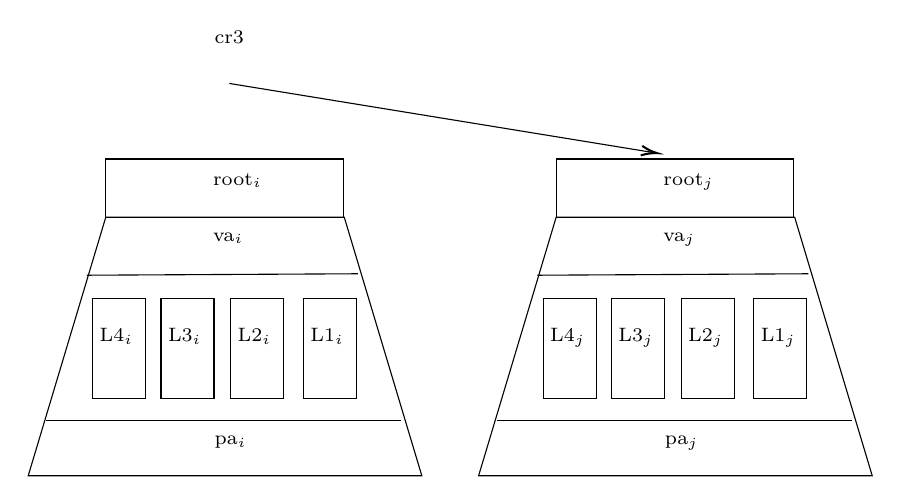
\begin{tikzpicture}[x=0.75pt,y=0.75pt,yscale=-0.7,xscale=0.7]
%uncomment if require: \path (0,444); %set diagram left start at 0, and has height of 444

%Straight Lines [id:da38505936382975436] 
\draw    (186,98) -- (478.53,145.68) ;
\draw [shift={(480.5,146)}, rotate = 189.26] [color={rgb, 255:red, 0; green, 0; blue, 0 }  ][line width=0.75]    (10.93,-3.29) .. controls (6.95,-1.4) and (3.31,-0.3) .. (0,0) .. controls (3.31,0.3) and (6.95,1.4) .. (10.93,3.29)   ;
%Shape: Trapezoid [id:dp7414076994636136] 
\draw   (47.6,368) -- (101,190) -- (265.1,190) -- (318.5,368) -- cycle ;
%Shape: Rectangle [id:dp6682076995791875] 
\draw   (101,150) -- (264.5,150) -- (264.5,190) -- (101,190) -- cycle ;
%Straight Lines [id:da13111570073586742] 
\draw    (88,230) -- (274.5,229) ;
%Straight Lines [id:da8088550891516297] 
\draw    (60,330) -- (304.5,330) ;
%Shape: Rectangle [id:dp21836577048687023] 
\draw   (92,246) -- (128.5,246) -- (128.5,315) -- (92,315) -- cycle ;
%Shape: Rectangle [id:dp057930941757168064] 
\draw   (139,246) -- (175.5,246) -- (175.5,315) -- (139,315) -- cycle ;
%Shape: Rectangle [id:dp39663188007381556] 
\draw   (187,246) -- (223.5,246) -- (223.5,315) -- (187,315) -- cycle ;
%Shape: Rectangle [id:dp5224337498132685] 
\draw   (237,246) -- (273.5,246) -- (273.5,315) -- (237,315) -- cycle ;
%Shape: Trapezoid [id:dp471852322248028] 
\draw   (357.6,368) -- (411,190) -- (575.1,190) -- (628.5,368) -- cycle ;
%Shape: Rectangle [id:dp5528716184490898] 
\draw   (411,150) -- (574.5,150) -- (574.5,190) -- (411,190) -- cycle ;
%Straight Lines [id:da7602460644496329] 
\draw    (398,230) -- (584.5,229) ;
%Straight Lines [id:da6992377024554963] 
\draw    (370,330) -- (614.5,330) ;
%Shape: Rectangle [id:dp8266326943417694] 
\draw   (402,246) -- (438.5,246) -- (438.5,315) -- (402,315) -- cycle ;
%Shape: Rectangle [id:dp6075494266540686] 
\draw   (449,246) -- (485.5,246) -- (485.5,315) -- (449,315) -- cycle ;
%Shape: Rectangle [id:dp7706384125026737] 
\draw   (497,246) -- (533.5,246) -- (533.5,315) -- (497,315) -- cycle ;
%Shape: Rectangle [id:dp6101896478605242] 
\draw   (547,246) -- (583.5,246) -- (583.5,315) -- (547,315) -- cycle ;

% Text Node
\draw (174,60) node [anchor=north west][inner sep=0.75pt]   [align=left] {{\scriptsize cr3}};
% Text Node
\draw (173,199) node [anchor=north west][inner sep=0.75pt]   [align=left] {{\scriptsize va$_i$}};
% Text Node
\draw (174,339) node [anchor=north west][inner sep=0.75pt]   [align=left] {{\scriptsize pa$_i$}};
% Text Node
\draw (95,265) node [anchor=north west][inner sep=0.75pt]   [align=left] {{\scriptsize L4$_i$}};
% Text Node
\draw (173,158) node [anchor=north west][inner sep=0.75pt]   [align=left] {{\scriptsize root$_i$}};
% Text Node
\draw (142,265) node [anchor=north west][inner sep=0.75pt]   [align=left] {{\scriptsize L3$_i$}};
% Text Node
\draw (190,265) node [anchor=north west][inner sep=0.75pt]   [align=left] {{\scriptsize L2$_i$}};
% Text Node
\draw (240,265) node [anchor=north west][inner sep=0.75pt]   [align=left] {{\scriptsize L1$_i$}};
% Text Node
\draw (483,199) node [anchor=north west][inner sep=0.75pt]   [align=left] {{\scriptsize va$_j$}};
% Text Node
\draw (484,339) node [anchor=north west][inner sep=0.75pt]   [align=left] {{\scriptsize pa$_j$}};
% Text Node
\draw (405,265) node [anchor=north west][inner sep=0.75pt]   [align=left] {{\scriptsize L4$_j$}};
% Text Node
\draw (483,158) node [anchor=north west][inner sep=0.75pt]   [align=left] {{\scriptsize root$_j$}};
% Text Node
\draw (452,265) node [anchor=north west][inner sep=0.75pt]   [align=left] {{\scriptsize L3$_j$}};
% Text Node
\draw (500,265) node [anchor=north west][inner sep=0.75pt]   [align=left] {{\scriptsize L2$_j$}};
% Text Node
\draw (550,265) node [anchor=north west][inner sep=0.75pt]   [align=left] {{\scriptsize L1$_j$}};


\end{tikzpicture}
        \caption{Switching Address-Spaces}
        \label{fig:enter-label}
    \end{figure}
\end{frame}
\begin{frame}{Managing Agnostic Memory Mappings}
\begin{columns}
\column{0.65\textwidth}    
    \begin{figure}
        \centering
\tikzset{every picture/.style={line width=0.75pt}} %set default line width to 0.75pt        

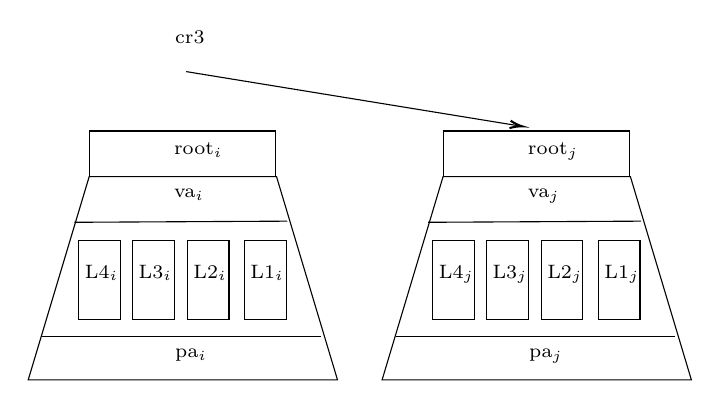
\begin{tikzpicture}[x=0.75pt,y=0.75pt,yscale=-0.55,xscale=0.55]
%uncomment if require: \path (0,444); %set diagram left start at 0, and has height of 444

%Straight Lines [id:da38505936382975436] 
\draw    (186,98) -- (478.53,145.68) ;
\draw [shift={(480.5,146)}, rotate = 189.26] [color={rgb, 255:red, 0; green, 0; blue, 0 }  ][line width=0.75]    (10.93,-3.29) .. controls (6.95,-1.4) and (3.31,-0.3) .. (0,0) .. controls (3.31,0.3) and (6.95,1.4) .. (10.93,3.29)   ;
%Shape: Trapezoid [id:dp7414076994636136] 
\draw   (47.6,368) -- (101,190) -- (265.1,190) -- (318.5,368) -- cycle ;
%Shape: Rectangle [id:dp6682076995791875] 
\draw   (101,150) -- (264.5,150) -- (264.5,190) -- (101,190) -- cycle ;
%Straight Lines [id:da13111570073586742] 
\draw    (88,230) -- (274.5,229) ;
%Straight Lines [id:da8088550891516297] 
\draw    (60,330) -- (304.5,330) ;
%Shape: Rectangle [id:dp21836577048687023] 
\draw   (92,246) -- (128.5,246) -- (128.5,315) -- (92,315) -- cycle ;
%Shape: Rectangle [id:dp057930941757168064] 
\draw   (139,246) -- (175.5,246) -- (175.5,315) -- (139,315) -- cycle ;
%Shape: Rectangle [id:dp39663188007381556] 
\draw   (187,246) -- (223.5,246) -- (223.5,315) -- (187,315) -- cycle ;
%Shape: Rectangle [id:dp5224337498132685] 
\draw   (237,246) -- (273.5,246) -- (273.5,315) -- (237,315) -- cycle ;
%Shape: Trapezoid [id:dp471852322248028] 
\draw   (357.6,368) -- (411,190) -- (575.1,190) -- (628.5,368) -- cycle ;
%Shape: Rectangle [id:dp5528716184490898] 
\draw   (411,150) -- (574.5,150) -- (574.5,190) -- (411,190) -- cycle ;
%Straight Lines [id:da7602460644496329] 
\draw    (398,230) -- (584.5,229) ;
%Straight Lines [id:da6992377024554963] 
\draw    (370,330) -- (614.5,330) ;
%Shape: Rectangle [id:dp8266326943417694] 
\draw   (402,246) -- (438.5,246) -- (438.5,315) -- (402,315) -- cycle ;
%Shape: Rectangle [id:dp6075494266540686] 
\draw   (449,246) -- (485.5,246) -- (485.5,315) -- (449,315) -- cycle ;
%Shape: Rectangle [id:dp7706384125026737] 
\draw   (497,246) -- (533.5,246) -- (533.5,315) -- (497,315) -- cycle ;
%Shape: Rectangle [id:dp6101896478605242] 
\draw   (547,246) -- (583.5,246) -- (583.5,315) -- (547,315) -- cycle ;

% Text Node
\draw (174,60) node [anchor=north west][inner sep=0.75pt]   [align=left] {{\scriptsize cr3}};
% Text Node
\draw (173,199) node [anchor=north west][inner sep=0.75pt]   [align=left] {{\scriptsize va$_i$}};
% Text Node
\draw (174,339) node [anchor=north west][inner sep=0.75pt]   [align=left] {{\scriptsize pa$_i$}};
% Text Node
\draw (95,265) node [anchor=north west][inner sep=0.75pt]   [align=left] {{\scriptsize L4$_i$}};
% Text Node
\draw (173,158) node [anchor=north west][inner sep=0.75pt]   [align=left] {{\scriptsize root$_i$}};
% Text Node
\draw (142,265) node [anchor=north west][inner sep=0.75pt]   [align=left] {{\scriptsize L3$_i$}};
% Text Node
\draw (190,265) node [anchor=north west][inner sep=0.75pt]   [align=left] {{\scriptsize L2$_i$}};
% Text Node
\draw (240,265) node [anchor=north west][inner sep=0.75pt]   [align=left] {{\scriptsize L1$_i$}};
% Text Node
\draw (483,199) node [anchor=north west][inner sep=0.75pt]   [align=left] {{\scriptsize va$_j$}};
% Text Node
\draw (484,339) node [anchor=north west][inner sep=0.75pt]   [align=left] {{\scriptsize pa$_j$}};
% Text Node
\draw (405,265) node [anchor=north west][inner sep=0.75pt]   [align=left] {{\scriptsize L4$_j$}};
% Text Node
\draw (483,158) node [anchor=north west][inner sep=0.75pt]   [align=left] {{\scriptsize root$_j$}};
% Text Node
\draw (452,265) node [anchor=north west][inner sep=0.75pt]   [align=left] {{\scriptsize L3$_j$}};
% Text Node
\draw (500,265) node [anchor=north west][inner sep=0.75pt]   [align=left] {{\scriptsize L2$_j$}};
% Text Node
\draw (550,265) node [anchor=north west][inner sep=0.75pt]   [align=left] {{\scriptsize L1$_j$}};


\end{tikzpicture}
        \caption{Switching Address-Spaces}
        \label{fig:enter-label}
    \end{figure}
     \column{0.375\textwidth}
    \begin{alertblock}{Referring to Agnostic Resources}
    Unless we bookkeep to which address-space each of these virtual-to-physical mappings belongs,  \emph{which we never see in the practice of using virtual memory references}, we need to figure out a way of referring to these mappings as \emph{they are only valid in their own address-spaces}.
    \end{alertblock}
    \end{columns}
\end{frame}
\section{Logic}
\subsection{A Quick Tour on Separation Logic (\textbf{SL})}
\begin{frame}{Specifying Programs}
    \[\{P\}\; C\; \{Q\} \]
\end{frame}
\begin{frame}{Separation Logic: Separating Conjuction}
   \[
\inferrule[Frame]{
	\triple{P}{e}{Q}
}{
	\triple{P\ast R}{e}{Q\ast R}
}
\]
\end{frame}
\begin{frame}{Separation Logic: Ownership}
    \begin{itemize}
        \item Well-known points-to assertion, e.g., $\mathsf{memory\_ref}\; \mapsto_{q} \;\mathsf{val}$
        \item Regarding the logical machinery, Iris \textbf{SL} enables encoding a generalized form ownership of \emph{logical resources}
        \item A fragmental $\ownGhost{\gamma}{P}$ ownership
            \begin{itemize}
            \item Enabling coordinated access to logical resources \end{itemize}
        \item Full $ \fbox{$P$}^\gamma$ ownership 
         \begin{itemize}
            \item Enabling access to \emph{update} logical resources, presented as \emph{invariants}
             \end{itemize}
    \end{itemize}
\end{frame}
\begin{frame}{Separation Logic: Invariants}
\[
    \inferrule[Inv]{
        \triple{  P \ast R }{\alpha}{P \ast Q }_{\epsilon}\\
        \alpha~\textrm{physically atomic}
    }{
        \fbox{$P$}^n \vdash \triple{ R }{\alpha}{ Q }_{\epsilon \uplus \{n\}}
    }
    \]
\end{frame}
\subsection{A Logic for Recovering the Soundness of Page-Table Traversal}
\begin{frame}{Defining Some Ownersip Assertions}
    \begin{itemize}
    \item   Expected to have register ownership to be defined : $\mathsf{reg} \; \mapsto_{r} \; \mathsf{reg\_val}$
        \item Expected to have \emph{physical memory} ownership defined: $\mathsf{pa} \; \mapsto_{p} \; \mathsf{val}$
        \item How about virtual memory references?
    \end{itemize}
\end{frame}
\begin{frame}{A Naive Attempt on Virtual-Pointsto}
    \begin{itemize}
        \item Page and page table addresses are \emph{physical}
        \item Purple (or red) path + bold black page references are \emph{physical}
        \item Why don't we define \emph{virtual} memory references in terms of the physical page-table and the final page references? 
    \end{itemize}
      \[ \textsf{L}_{4}\_\textsf{L}_{1}\_\textsf{PointsTo}(\vaddr\textsf{, l4e, l3e, l2e, l1e, paddr}) + paddr \mapsto_{p} \mathsf{page\_val}\]
%
%          \text{\Large                    No!}
%
\end{frame}
\begin{frame}{Tokens for Traversals} \scriptsize
    \begin{columns}
        \column{0.5\textwidth}
\[        \underbrace{\fracghostmaptoken{\delta}{\vaddr}{\paddr}{\qfrac} }_\text{Ghost translation} \ast \underbrace{\paddr \mapsto_{\mathsf{p}}\{\textsf{qfrac}\}\; \vale}_\text{Physical location} \]
        \column{0.5\textwidth}
        \begin{itemize}
            \item Abstract the purple and red segment of page-table traversal into \emph{logical summarization of the walk}
            \item Distribute the fragmental ownersip of the logical page-table summarization to virtual memory ownership
        \end{itemize}
    \end{columns}
\end{frame}
\begin{frame}{A Candidate for Kernel Invariant}
     \begin{figure}
  \scriptsize
\centerline{$
\begin{array}{l}
  \mathcal{I}\textsf{ASpace}(\ptablestore,m)\stackrel{\triangle}{=} \textsf{ASpace\_Lookup}(\ptablestore,m) \ast \\
 \qquad\qquad\qquad \bigast{(\vaddr, \textsf{paddr})\in \ptablestore}{\exists\;(\textsf{l4e l3e l2e, l1e, paddr})\ldotp \textsf{L}_{4}\_\textsf{L}_{1}\_\textsf{PointsTo}(\vaddr\textsf{, l4e, l3e, l2e, l1e, paddr})} \\
  \textsf{ where } \\
   \textsf{ASpace\_Lookup} (\ptablestore,m) \stackrel{\triangle}{=} \lambda\textsf{ cr3val} \ldotp \; \exists \gammaPred \; \ldotp \ulcorner m \; !!\; \textsf{cr3val} = \textsf{Some } \gammaPred \urcorner \ast
    %\ownGhost\gammaPred{\authfull{\ptableabswalk\ptablestore}}
    \ptableabswalk{\delta,\theta}
\end{array}
$}
\caption{Global Address-Space Invariant with a fixed global map of address-space names $m$}
  \label{fig:peraspaceinvariant}
  \end{figure}
\end{frame}
\begin{frame}{A Candidate for Kernel Invariant}
    \begin{alertblock}{The Kernel Invariant in Action}
    How useful (complete) is this invariant?
    \end{alertblock}
\end{frame}
\begin{frame}[fragile]{Kernels Locating L1 Entries}\scriptsize
    \begin{columns}[c]
\column{.59\textwidth}    
    \begin{figure}
        \centering
    


\tikzset{every picture/.style={line width=0.75pt}} %set default line width to 0.75pt        

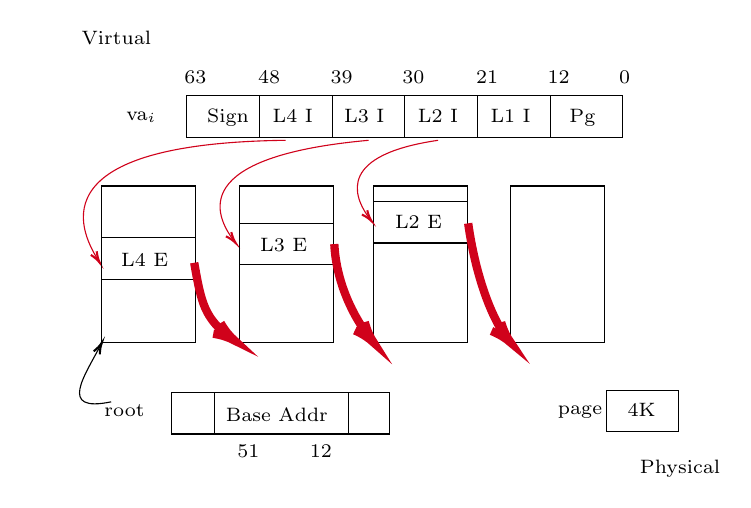
\begin{tikzpicture}[x=0.75pt,y=0.75pt,yscale=-0.5,xscale=0.5]
%uncomment if require: \path (0,461); %set diagram left start at 0, and has height of 461

%Shape: Rectangle [id:dp8985266189265282] 
\draw   (30,162) -- (120,162) -- (120,313) -- (30,313) -- cycle ;
%Shape: Rectangle [id:dp8580905480423404] 
\draw   (163,162) -- (253,162) -- (253,313) -- (163,313) -- cycle ;
%Shape: Rectangle [id:dp04681279805293914] 
\draw   (292,162) -- (382,162) -- (382,313) -- (292,313) -- cycle ;
%Shape: Rectangle [id:dp7764939174959982] 
\draw   (424,162) -- (514,162) -- (514,313) -- (424,313) -- cycle ;
%Shape: Rectangle [id:dp5300844634901585] 
\draw   (112,75) -- (182,75) -- (182,115) -- (112,115) -- cycle ;
%Shape: Rectangle [id:dp4415280160774133] 
\draw   (182,75) -- (252,75) -- (252,115) -- (182,115) -- cycle ;
%Shape: Rectangle [id:dp2994535835985157] 
\draw   (252,75) -- (322,75) -- (322,115) -- (252,115) -- cycle ;
%Shape: Rectangle [id:dp32418137012170356] 
\draw   (322,75) -- (392,75) -- (392,115) -- (322,115) -- cycle ;
%Shape: Rectangle [id:dp37951844906888543] 
\draw   (392,75) -- (462,75) -- (462,115) -- (392,115) -- cycle ;
%Shape: Rectangle [id:dp6243329849126165] 
\draw   (462,75) -- (532,75) -- (532,115) -- (462,115) -- cycle ;
%Curve Lines [id:da5300291149539194] 
\draw [color={rgb, 255:red, 208; green, 2; blue, 27 }  ,draw opacity=1 ]   (207,118) .. controls (-40.94,120.94) and (12.69,211.28) .. (27.17,234.65) ;
\draw [shift={(28,236)}, rotate = 238.24] [color={rgb, 255:red, 208; green, 2; blue, 27 }  ,draw opacity=1 ][line width=0.75]    (10.93,-3.29) .. controls (6.95,-1.4) and (3.31,-0.3) .. (0,0) .. controls (3.31,0.3) and (6.95,1.4) .. (10.93,3.29)   ;
%Shape: Rectangle [id:dp6164472725736567] 
\draw   (30,212) -- (120,212) -- (120,252) -- (30,252) -- cycle ;
%Curve Lines [id:da23035098640096874] 
\draw [color={rgb, 255:red, 208; green, 2; blue, 27 }  ,draw opacity=1 ]   (287,118) .. controls (113.54,133.68) and (137.92,189.7) .. (157.79,215.46) ;
\draw [shift={(159,217)}, rotate = 231.34] [color={rgb, 255:red, 208; green, 2; blue, 27 }  ,draw opacity=1 ][line width=0.75]    (10.93,-3.29) .. controls (6.95,-1.4) and (3.31,-0.3) .. (0,0) .. controls (3.31,0.3) and (6.95,1.4) .. (10.93,3.29)   ;
%Shape: Rectangle [id:dp6844649352396941] 
\draw   (163,198) -- (253,198) -- (253,238) -- (163,238) -- cycle ;
%Shape: Rectangle [id:dp14248498609413196] 
\draw   (292,177) -- (382,177) -- (382,217) -- (292,217) -- cycle ;
%Curve Lines [id:da681101715887759] 
\draw [color={rgb, 255:red, 208; green, 2; blue, 27 }  ,draw opacity=1 ]   (354,118) .. controls (259.92,131.72) and (269.56,169.45) .. (288.81,194.48) ;
\draw [shift={(290,196)}, rotate = 231.34] [color={rgb, 255:red, 208; green, 2; blue, 27 }  ,draw opacity=1 ][line width=0.75]    (10.93,-3.29) .. controls (6.95,-1.4) and (3.31,-0.3) .. (0,0) .. controls (3.31,0.3) and (6.95,1.4) .. (10.93,3.29)   ;
%Curve Lines [id:da7448745938095696] 
\draw    (39,370) .. controls (-13.21,380.84) and (14.15,344.13) .. (29.32,314.36) ;
\draw [shift={(30,313)}, rotate = 116.57] [color={rgb, 255:red, 0; green, 0; blue, 0 }  ][line width=0.75]    (10.93,-3.29) .. controls (6.95,-1.4) and (3.31,-0.3) .. (0,0) .. controls (3.31,0.3) and (6.95,1.4) .. (10.93,3.29)   ;
%Curve Lines [id:da22392385009085425] 
\draw [color={rgb, 255:red, 208; green, 2; blue, 27 }  ,draw opacity=1 ][line width=3]    (119,236) .. controls (125.69,274.2) and (128.72,289.6) .. (154.24,308.33) ;
\draw [shift={(158,311)}, rotate = 214.59] [color={rgb, 255:red, 208; green, 2; blue, 27 }  ,draw opacity=1 ][line width=3]    (20.77,-6.25) .. controls (13.2,-2.65) and (6.28,-0.57) .. (0,0) .. controls (6.28,0.57) and (13.2,2.66) .. (20.77,6.25)   ;
%Curve Lines [id:da7384001101529021] 
\draw [color={rgb, 255:red, 208; green, 2; blue, 27 }  ,draw opacity=1 ][line width=3]    (254,218) .. controls (255.88,255.6) and (272.78,288.78) .. (288.92,309.24) ;
\draw [shift={(292,313)}, rotate = 229.64] [color={rgb, 255:red, 208; green, 2; blue, 27 }  ,draw opacity=1 ][line width=3]    (20.77,-6.25) .. controls (13.2,-2.65) and (6.28,-0.57) .. (0,0) .. controls (6.28,0.57) and (13.2,2.66) .. (20.77,6.25)   ;
%Curve Lines [id:da461641424558785] 
\draw [color={rgb, 255:red, 208; green, 2; blue, 27 }  ,draw opacity=1 ][line width=3]    (383,198) .. controls (389.62,245.25) and (404.27,288.03) .. (421.05,309.48) ;
\draw [shift={(424,313)}, rotate = 228.01] [color={rgb, 255:red, 208; green, 2; blue, 27 }  ,draw opacity=1 ][line width=3]    (20.77,-6.25) .. controls (13.2,-2.65) and (6.28,-0.57) .. (0,0) .. controls (6.28,0.57) and (13.2,2.66) .. (20.77,6.25)   ;
%Shape: Rectangle [id:dp7456876017683469] 
\draw   (516,359) -- (586,359) -- (586,399) -- (516,399) -- cycle ;
%Shape: Rectangle [id:dp44145929649929916] 
\draw   (97,361) -- (138.5,361) -- (138.5,401) -- (97,401) -- cycle ;
%Shape: Rectangle [id:dp6608975412508127] 
\draw   (138.5,361) -- (267.5,361) -- (267.5,401) -- (138.5,401) -- cycle ;
%Shape: Rectangle [id:dp927545333863445] 
\draw   (267.5,361) -- (307,361) -- (307,401) -- (267.5,401) -- cycle ;

% Text Node
\draw (8,10) node [anchor=north west][inner sep=0.75pt]   [align=left] {{\scriptsize Virtual}};
% Text Node
\draw (546,424) node [anchor=north west][inner sep=0.75pt]   [align=left] {{\scriptsize Physical}};
% Text Node
\draw (129,86) node [anchor=north west][inner sep=0.75pt]   [align=left] {{\scriptsize Sign}};
% Text Node
\draw (192,86) node [anchor=north west][inner sep=0.75pt]   [align=left] {{\scriptsize L4 I}};
% Text Node
\draw (261,86) node [anchor=north west][inner sep=0.75pt]   [align=left] {{\scriptsize L3 I}};
% Text Node
\draw (332,86) node [anchor=north west][inner sep=0.75pt]   [align=left] {{\scriptsize L2 I}};
% Text Node
\draw (402,86) node [anchor=north west][inner sep=0.75pt]   [align=left] {{\scriptsize L1 I}};
% Text Node
\draw (478,86) node [anchor=north west][inner sep=0.75pt]   [align=left] {{\scriptsize Pg}};
% Text Node
\draw (51,88) node [anchor=north west][inner sep=0.75pt]   [align=left] {{\scriptsize va$_i$}};
% Text Node
\draw (30,370) node [anchor=north west][inner sep=0.75pt]   [align=left] {{\scriptsize root}};
% Text Node
\draw (46,224) node [anchor=north west][inner sep=0.75pt]   [align=left] {{\scriptsize L4 E}};
% Text Node
\draw (180,210) node [anchor=north west][inner sep=0.75pt]   [align=left] {{\scriptsize L3 E}};
% Text Node
\draw (310,188) node [anchor=north west][inner sep=0.75pt]   [align=left] {{\scriptsize L2 E}};
% Text Node
\draw (467,372) node [anchor=north west][inner sep=0.75pt]   [align=left] {{\scriptsize page}};
% Text Node
\draw (534,369) node [anchor=north west][inner sep=0.75pt]   [align=left] {{\scriptsize 4K}};
% Text Node
\draw (158,409) node [anchor=north west][inner sep=0.75pt]   [align=left] {{\scriptsize 51}};
% Text Node
\draw (228,409) node [anchor=north west][inner sep=0.75pt]   [align=left] {{\scriptsize 12}};
% Text Node
\draw (147,373) node [anchor=north west][inner sep=0.75pt]   [align=left] {{\scriptsize Base Addr}};
% Text Node
\draw (107,49) node [anchor=north west][inner sep=0.75pt]   [align=left] {{\scriptsize 63}};
% Text Node
\draw (178,49) node [anchor=north west][inner sep=0.75pt]   [align=left] {{\scriptsize 48}};
% Text Node
\draw (248,49) node [anchor=north west][inner sep=0.75pt]   [align=left] {{\scriptsize 39}};
% Text Node
\draw (317,49) node [anchor=north west][inner sep=0.75pt]   [align=left] {{\scriptsize 30}};
% Text Node
\draw (388,49) node [anchor=north west][inner sep=0.75pt]   [align=left] {{\scriptsize 21}};
% Text Node
\draw (457,49) node [anchor=north west][inner sep=0.75pt]   [align=left] {{\scriptsize 12}};
% Text Node
\draw (526,49) node [anchor=north west][inner sep=0.75pt]   [align=left] {{\scriptsize 0}};


\end{tikzpicture}
    %    \caption{Caption}
    %    \label{fig:enter-label}
    \end{figure}
    \column{.4\textwidth}
\begin{lstlisting}[style=CStyleNumEmph, basicstyle=\tiny]
static pte_t *pte_nxt_table (pte_t *entry){
 pte_t *next;
 // If not already present, try to allocate
 if (!entry->present){
  if (!pte_alloc(&next)) {
   return NULL;
  }
  entry->pfn = PTE_PFN((uintptr_t) next);
  entry->present = 1;
  } else {
   \uintptr_t next_phys_addr = PTE_PFN_TO_ADDR(entry->pfn);        
   uintptr_t next_virt_addr = (uintptr_t) P2V(next_phys_addr);
   next = (pte_t *) next_virt_addr;
  }
  return next;
}   
pte_t *walkpgdir(pte_t *l4, void *va){ 
 pte_t *l4_entry = &l4[L4I(va)];
 pte_t *l3 = pte_nxt_table(l4_entry);
 pte_t *l3_entry = &l3[L3I(va)];
 pte_t *l2 = pte_nxt_table(l3_entry);
 pte_t *l2_entry = &l2[L2I(va)];  
 pte_t *l1 = pte_nxt_table(l2_entry);
 pte_t *l1_entry = &l1[L1I(va)];  
}
\end{lstlisting}
\end{columns}
\end{frame}

\begin{frame}{Incorporating \textbf{P2V} into the Kernel Invariant}\scriptsize
    \begin{definition}[The Kernel Invariant for Page-Table Traversal with Virtual Page-Table Pointers]
        
\[
\begin{array}{l}
  \mathcal{I}\textsf{ASpace}_{\textsf{id}}(\ptablestore,\Xi,m)\stackrel{\triangle}{=} \textsf{ASpace\_Lookup}_{\textsf{id}}(\ptablestore,\Xi,m) \ast \mathsf{GhostMap}(\mathsf{id},\Xi)\ast\\
  \left(\bigast{(\vaddr, \textsf{paddr})\in \ptablestore}{\exists\;(\textsf{l4e, l3e, l2e, l1e, paddr})\ldotp \textsf{L}_{4}\_\textsf{L}_{1}\_\textsf{PointsTo}(\vaddr\textsf{, l4e, l3e, l2e, l1e, paddr})}\right)\ast \\
  \bigast{(\paddr,\mathsf{level}) \in \Xi}{\exists\; (\textsf{qfrac, q, val,}\vaddr) \ldotp \ulcorner \vaddr = \paddr + \textsf{KERNBASE} \; \textsf{level} > 1\urcorner \ast  \underbrace{\fracghostmaptoken{\delta}{\vaddr}{\paddr}{\qfrac} }_\text{Ghost translation} \ast \underbrace{\paddr \mapsto_{\mathsf{p}}\{\textsf{qfrac}\}\; \vale}_\text{Physical location}} \ast\\
   \qquad\underbrace{ \ulcorner \textsf{qfrac} = 1 \leftrightarrow \; \lnot\textsf{entry\_present }(\vale) \urcorner}_\text{Entry validity}\ast \\
    \underbrace{\left(\ulcorner\textsf{present\_L}(\vale,\mathsf{level})\urcorner \wand \forall_{\textsf{i}\in\textsf{0..511}} \ldotp \ghostmaptoken{\textsf{id}}{((\mathsf{entry\_page}\;\vale) + \textsf{i * 8})}{\textsf{level-1}}\right)}_{\text{Indexing into next level of tables}} \\ %\\
  \textsf{ where } \\
%   \textsf{ASpace\_Lookup}_{\textsf{id}}(\ptablestore,\Xi,m) \stackrel{\triangle}{=} \lambda\textsf{ cr3val} \ldotp \; \exists \gammaPred \; \ldotp \ulcorner m \; !!\; \textsf{cr3val} = \textsf{Some } \gammaPred \urcorner \ast
   % \ownGhost\gammaPred{\authfull{\ptableabswalk\ptablestore}} \ast  \ownGhostpv\gammaPred{\authfull{\pvmapping\Xi}}
 %  \ptableabswalk{\delta,\ptablestore} \ast \pvmapping{\delta,\Xi}\\
  \textsf{present\_L}(\vale,\mathsf{level})\stackrel{\triangle}{=} \mathsf{entry\_present}(\vale)\land \mathsf{level} > 0
  
\end{array}
\]
\end{definition}
\end{frame}
\begin{frame}[fragile]{Specifying \textsf{P2V}}\scriptsize
    \begin{figure}\scriptsize
\begin{lstlisting}[mathescape,escapeinside={(*}{*)}]
$\specline{\textsf{P} \ast \mathcal{I}\texttt{ASpace}_{\textsf{id}}(\theta,\Xi\setminus \{ \mathsf{entry} \}),m)  \ast \textsf{rbp-8} \mapsto_{\textsf{v}} \textsf{entry} \ast \texttt{rcx}  \mapsto_{\textsf{r}} \textsf{\_}  \ast \textsf{entry} \mapsto_{\textsf{id}} \textsf{\_} \ast \ghostmaptoken{\delta{}s}{\rtv}{\delta}  }_{\rtv}$
$\specline{ \textsf{entry+KERNBASE} \mapsto_{\textsf{vpte,qfrac}} \textsf{(pte\_initialized (entry\_val.pfn))} \urcorner }_{\rtv}$
$\specline{ \texttt{rbp-16} \mapsto_{\textsf{v}} \textsf{(pte\_initialized (entry\_val.pfn)))} \ast \texttt{rax} \mapsto_{\textsf{r}} \textsf{ table\_root (pte\_initialize(entry\_val.pfn))} }_{\rtv}$
$\specline{\forall_{i\in \textsf{0 ... 511} } \ldotp  \ghostmaptoken{\textsf{id}}{((\textsf{table\_root (pte\_initialized (entry\_val.pfn)))}) + \textsf{i * 8})}{\textsf{v-1}}  }$ (*\label{line:children}*)
;;uintptr_t next_virt_addr = (uintptr_t) P2V(entry.pfn<<12); (*\label{line:p2v}*) 
movabs KERNBASE,rcx $\specline{\ldots \ast  \texttt{rcx}  \mapsto_{\textsf{r}} \textsf{KERNBASE}  \ast \ldots}_{\rtv}$
add    rcx,rax
$\specline{ \ldots \ast \texttt{rax} \mapsto_{\textsf{r}} \textsf{ table\_root (pte\_initialize(entry\_val.pfn)) + KERNBASE}  \ast \ldots}_{\rtv}$
... ;;clean up the stack and return the rax value
\end{lstlisting}
\caption{Converting a physical address of a PTE to a virtual address (w/o instruction pointer or flag updates).}
\label{fig:p2v}
\end{figure}
\end{frame}
\subsection{A Logic of Agnostic Resources}
\section{The Verification Effort}
\subsection{Design}
\begin{frame}{The Current Status of Machinery}\scriptsize
\begin{columns}
\column{0.65\textwidth}    
    \begin{figure}
        \centering
    \tikzset{every picture/.style={line width=0.75pt}} %set default line width to 0.75pt        
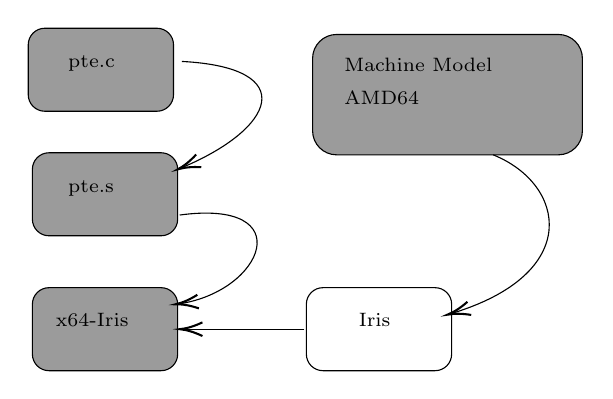
\begin{tikzpicture}[x=0.75pt,y=0.75pt,yscale=-1,xscale=1]
%uncomment if require: \path (0,201); %set diagram left start at 0, and has height of 201

%Rounded Rect [id:dp9674022449831219] 
\draw  [fill={rgb, 255:red, 155; green, 155; blue, 155 }  ,fill opacity=1 ] (49,141) .. controls (49,136.58) and (52.58,133) .. (57,133) -- (111,133) .. controls (115.42,133) and (119,136.58) .. (119,141) -- (119,165) .. controls (119,169.42) and (115.42,173) .. (111,173) -- (57,173) .. controls (52.58,173) and (49,169.42) .. (49,165) -- cycle ;
%Rounded Rect [id:dp2624123472522688] 
\draw   (181,141) .. controls (181,136.58) and (184.58,133) .. (189,133) -- (243,133) .. controls (247.42,133) and (251,136.58) .. (251,141) -- (251,165) .. controls (251,169.42) and (247.42,173) .. (243,173) -- (189,173) .. controls (184.58,173) and (181,169.42) .. (181,165) -- cycle ;
%Rounded Rect [id:dp6259709693060862] 
\draw  [fill={rgb, 255:red, 155; green, 155; blue, 155 }  ,fill opacity=1 ] (49,76) .. controls (49,71.58) and (52.58,68) .. (57,68) -- (111,68) .. controls (115.42,68) and (119,71.58) .. (119,76) -- (119,100) .. controls (119,104.42) and (115.42,108) .. (111,108) -- (57,108) .. controls (52.58,108) and (49,104.42) .. (49,100) -- cycle ;
%Rounded Rect [id:dp01887654130349059] 
\draw  [fill={rgb, 255:red, 155; green, 155; blue, 155 }  ,fill opacity=1 ] (184,22.6) .. controls (184,16.19) and (189.19,11) .. (195.6,11) -- (302.4,11) .. controls (308.81,11) and (314,16.19) .. (314,22.6) -- (314,57.4) .. controls (314,63.81) and (308.81,69) .. (302.4,69) -- (195.6,69) .. controls (189.19,69) and (184,63.81) .. (184,57.4) -- cycle ;
%Rounded Rect [id:dp43251333121558844] 
\draw  [fill={rgb, 255:red, 155; green, 155; blue, 155 }  ,fill opacity=1 ] (47,16) .. controls (47,11.58) and (50.58,8) .. (55,8) -- (109,8) .. controls (113.42,8) and (117,11.58) .. (117,16) -- (117,40) .. controls (117,44.42) and (113.42,48) .. (109,48) -- (55,48) .. controls (50.58,48) and (47,44.42) .. (47,40) -- cycle ;
%Curve Lines [id:da4125031251275959] 
\draw    (271,69) .. controls (305.83,82.93) and (314.91,126.56) .. (249.98,145.71) ;
\draw [shift={(249,146)}, rotate = 343.94] [color={rgb, 255:red, 0; green, 0; blue, 0 }  ][line width=0.75]    (10.93,-3.29) .. controls (6.95,-1.4) and (3.31,-0.3) .. (0,0) .. controls (3.31,0.3) and (6.95,1.4) .. (10.93,3.29)   ;
%Straight Lines [id:da4796300520719461] 
\draw    (180,153) -- (122,153) ;
\draw [shift={(120,153)}, rotate = 360] [color={rgb, 255:red, 0; green, 0; blue, 0 }  ][line width=0.75]    (10.93,-3.29) .. controls (6.95,-1.4) and (3.31,-0.3) .. (0,0) .. controls (3.31,0.3) and (6.95,1.4) .. (10.93,3.29)   ;
%Curve Lines [id:da6791394644184989] 
\draw    (121,24) .. controls (178.42,26.97) and (166.25,56.4) .. (120.4,75.43) ;
\draw [shift={(119,76)}, rotate = 337.99] [color={rgb, 255:red, 0; green, 0; blue, 0 }  ][line width=0.75]    (10.93,-3.29) .. controls (6.95,-1.4) and (3.31,-0.3) .. (0,0) .. controls (3.31,0.3) and (6.95,1.4) .. (10.93,3.29)   ;
%Curve Lines [id:da09850046696764791] 
\draw    (120,98) .. controls (178.12,90.12) and (160.55,134.63) .. (119.87,140.75) ;
\draw [shift={(118,141)}, rotate = 353.21] [color={rgb, 255:red, 0; green, 0; blue, 0 }  ][line width=0.75]    (10.93,-3.29) .. controls (6.95,-1.4) and (3.31,-0.3) .. (0,0) .. controls (3.31,0.3) and (6.95,1.4) .. (10.93,3.29)   ;

% Text Node
\draw (198,21) node [anchor=north west][inner sep=0.75pt]   [align=left] {\scriptsize Machine Model\\ \scriptsize AMD64};
% Text Node
\draw (205,144) node [anchor=north west][inner sep=0.75pt]   [align=left] {\scriptsize Iris};
% Text Node
\draw (59,144) node [anchor=north west][inner sep=0.75pt]   [align=left] {\scriptsize x64-Iris};
% Text Node
\draw (65,80) node [anchor=north west][inner sep=0.75pt]   [align=left] {\scriptsize pte.s};
% Text Node
\draw (65,20) node [anchor=north west][inner sep=0.75pt]   [align=left] {\scriptsize pte.c};


\end{tikzpicture}
        \caption{x64-Iris}
        \label{fig:enter-label}
    \end{figure}
    \column{0.34\textwidth}
    \begin{itemize}
        \item Dumping \textbf{.o} files
        \item Manuel treatment on \textbf{Xabs} instructions and field access
    \end{itemize}
    \end{columns}
\end{frame}
\begin{frame}{A Rough Quantification on the Current Status}\scriptsize
    \begin{table}[ht]
\centering
\caption{Line-of-Code Numbers for \textsf{pte} Verification}
\label{fig:tablepte}
\begin{tabular}[t]{lccc}
\hline
& C LoC A& Assembly LoC & Roqc Proof LoC \\
\hline
pte\_get\_next\_table&12&45& ~3200\\
pte\_walkpgdir&8&44& ~3200\\
pte\_p2v&--&1&~75\\
pte\_switch\_addrspace&--&18&~350\\
pte\_map\_page&7&28&~1750\\
pte\_initialize&4&20&~700\\
\hline
\end{tabular}
\end{table}%
\begin{table}[ht]
\centering
\caption{Line-of-Code Numbers for x64-Iris Logic}
\label{fig:tablex64iris}
\begin{tabular}[t]{lc}
\hline
& Roqc LoC  \\
\hline
Soundness of Instructions Mentioned in the Thesis &50176\\
VMM Related Logical Constructions &5554\\
Machine Model & 6172\\
\hline
\end{tabular}
\end{table}%

\end{frame}
\section{The Current and Future Directions \& Conclusions}
\subsection{Modal Abstractions for Verification Patterns}
%begin{frame}{Resource and its Context}
 %   \begin{definition}[Resource]
 %%   \end{definition}
   % \begin{definition}[Resource Context]
   % \end{definition}
   % \begin{definition}[Nominalization]
   % \end{definition}
%\end{frame}
%------------------
\begin{frame}{Modal Abstractions as Verification Patterns in Practice}
   \resizebox{\textwidth}{!}{%
\begin{tabular}{@{}ccccp{5cm}@{}}
\toprule
& Resource Context & Resource Elements  &  Nominalization & Resource Context Steps \\ \midrule
Post-Crash Modality ~\cite{tejthesis, perennialgit,tejperennial19} & $\Diamond \; P $  & $  \ell \mapsto_{n}^{\overline{\gamma}} v $ & Strong &  Crash Recovery   \\ 
%GC-Modality &      & \multicolumn{2}{c}{\multirow{2}{*}{Because why not}} & 8                                   & & ~\cite{}\\
NextGen Modality~\cite{larsnextgen25} &  $\overset{t}{\hookrightarrow} \; P$  & Own (t(a))  & Strong & Determined Based on the Model$^{*}$   \\
StackRegion  Modality$^{*}$  ~\cite{larsnextgen25} & $\overset{ICut^{n}}{\hookrightarrow} \; P$      & $\fbox{n} \; \ell \mapsto v$                                 & Strong & Alloc and Return to/from stack\\
Memory-Fence  Modality ~\cite{fsl,fsl++,derekrustbelt20} & $\triangle_{\pi}$ and $\triangledown_{\pi}$      & $\ell \mapsto v$                                 & Weak & Fence Acquire and Release  \\
Address-Space Modality ~\cite{kuru2024modalabstractionsvirtualizingmemory} & [r]P     &  $\ell \mapsto v$ & Weak                         & Address-Space Switch  \\ 
Ref-Count Modality ~\cite{amalreal2024}& @$_{\ell}$ P    &  $\ell_1 \mapsto v$ & Weak  & Allocating, Dropping and Sharing a Reference \\ \bottomrule
\end{tabular}
}
\begin{itemize}
\item The StackRegion Modality is an instance of NextGen (called the Independence Modality in \cite{larsnextgen25}).
\end{itemize}
\end{frame}
%--------------
\makepart{Modal Understanding of Specification Evolution}
\section{Definitions}
\begin{frame}{Specifying Protocols for Systems with \textbf{STS}es}\scriptsize
\begin{columns}[c]
\column{0.45\textwidth}
\begin{figure}
    \centering
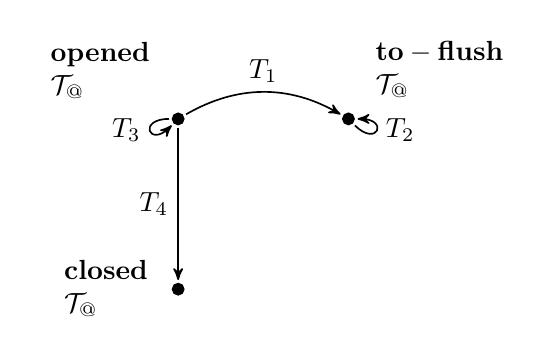
\begin{tikzpicture}[modal]
    \node[point] (to-flush) [label=135:{$\begin{array}{l}\mathbf{opened} \\ \mathcal{T}_@\end{array}$}] {};
    \node[point] (opened) [right=of to-flush, label=60:{$\begin{array}{l}\mathbf{to-flush}\\\mathcal{T}_@  
    \end{array}$}] {};
    \node[point](closed) [below=of to-flush, label=180:{$\begin{array}{l}\mathbf{closed}\\\mathcal{T}_@ 
    \end{array}$}] {};
    \path[->] (to-flush) edge[bend left] node[above]{$T_1$} (opened);
    \path[->] (opened) edge[reflexive right,out=-45,in=0,looseness=18] node[right] {$T_2$} (opened);
    \path[->] (to-flush) edge[reflexive left,out=180,in=225,looseness=18] node[left] {$T_3$} (to-flush);
     \path[->] (to-flush) edge node[left] {$T_4$} (closed);
\end{tikzpicture}
    \caption{STS for Distributed File Protocol}
    \label{fig:enter-label}
\end{figure}
\column{.45\textwidth}
\begin{figure}
    \centering
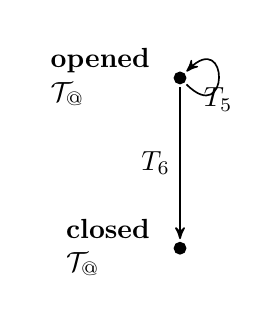
\begin{tikzpicture}[modal]
    \node[point] (opened) [label=left:{$\begin{array}{l}\mathbf{opened}\\ \mathcal{T}_@\end{array}$}] {};
     \node[point](closed) [below=of opened, label=180:{$\begin{array}{l}\mathbf{closed}\\\mathcal{T}_@ 
    \end{array}$}] {};
    \path[->] (opened) edge[reflexive right,out=-45,in=45,looseness=18] node[below] {$T_5$} (opened);
      \path[->] (opened) edge node[left] {$T_6$} (closed);
\end{tikzpicture}
    \caption{STS for Traditional File Protocol}
    \label{fig:enter-label}
    \end{figure}
\end{columns}
\begin{block}{Interacting with \textbf{STS}es}
 Modelling interactions of a client with a state machine via \emph{token exchange}
\end{block}
\end{frame}
%------------------------------------------------
\begin{frame}{Defining \textbf{STS}es}\scriptsize
\begin{definition}[\textbf{STS} Definition following CaReSL's presentation~\cite{turon13b}]
An STS $\pi$ is given by:
\begin{enumerate}
\item a set of states $\mathcal{S}$,
\item a map from a state set of tokens $\mathcal{T} : \mathcal{S} \rightarrow \mathsf{TokSet}$,
\item a transition relation $\leadsto$ on states, which is then lifted to pairs of a state and token set:
    \[(s;T)\leadsto(s';T') \triangleq s\leadsto s' \land \mathcal{T}(s)\uplus T = \mathcal{T}(s')\uplus T'\]
\item an interpretation mapping states to state assertions $\varphi :
    \mathcal{S}\rightarrow \mathsf{Prop}$.
    \end{enumerate}
\end{definition}
\end{frame}
\begin{frame}{Propositional Kripke Model}\scriptsize
     \begin{definition}[(Propositional) Kripke Model~\cite{hughes1996new}]
    A Kripke model $\mathfrak{M}$ is a triple $(W,R,V)$ where
    \begin{itemize}
        \item $W$ is a set of ``worlds''
        \item $R\subseteq W\times W$ is a relation called the \emph{accessibility} relation between worlds
        \item $V : \mathsf{PropVar} \rightarrow \mathcal{P}(W)$ gives for each propositional variable $p$ a set of worlds $V(p)$ where $p$ is considered true
    \end{itemize}
\end{definition}
\end{frame}
\begin{frame}{Bisimulations over Kripke Models}\scriptsize
\begin{definition}[(Propositional) Bisimulation of Kripke Structures: $\mathfrak{M}\sim\mathfrak{M}'$.]
    A \emph{bisimulation} between (multimodal) Kripke structures $(W,R_{i\in I},V)$ and $(W',R'_{i\in I},V')$ is a relation $E\subseteq W\times W'$ satisfying:
 \begin{itemize}
     \item If $w \; E \;w'$, then $w$ and $w'$ satisfy the same propositional variables.
     \item If $w \; E \;w'$ and $w \; R \; v$, then there exists $v'\in W'$ such that $v\;E\;v'$ and $w'\;R'\;v'$
       \item If $w \; E \;w'$ and $w'\;R'\;v'$, then there exists $v\in W$ such that $v\;R\;v'$ and $w\;R\;v$
    \end{itemize}   
\end{definition}
\end{frame}

\section{Motivation}
\subsection{Indistinguishability of Machines}
\begin{frame}{Intuition on Bisimulations over \textbf{STS}es}\scriptsize
\begin{columns}[c]
\column{0.45\textwidth}
\begin{figure}
    \centering
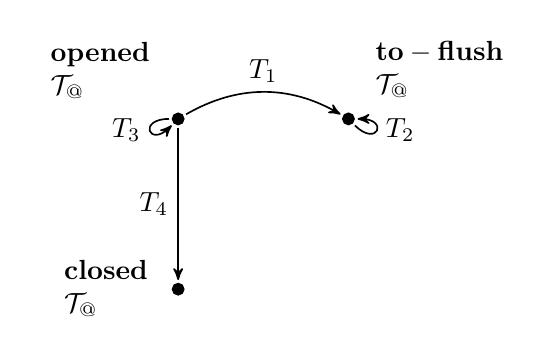
\begin{tikzpicture}[modal]
    \node[point] (to-flush) [label=135:{$\begin{array}{l}\mathbf{opened} \\ \mathcal{T}_@\end{array}$}] {};
    \node[point] (opened) [right=of to-flush, label=60:{$\begin{array}{l}\mathbf{to-flush}\\\mathcal{T}_@  
    \end{array}$}] {};
    \node[point](closed) [below=of to-flush, label=180:{$\begin{array}{l}\mathbf{closed}\\\mathcal{T}_@ 
    \end{array}$}] {};
    \path[->] (to-flush) edge[bend left] node[above]{$T_1$} (opened);
    \path[->] (opened) edge[reflexive right,out=-45,in=0,looseness=18] node[right] {$T_2$} (opened);
    \path[->] (to-flush) edge[reflexive left,out=180,in=225,looseness=18] node[left] {$T_3$} (to-flush);
     \path[->] (to-flush) edge node[left] {$T_4$} (closed);
\end{tikzpicture}
   % \caption{Caption}
    \label{fig:enter-label}
\end{figure}
\column{.45\textwidth}
\begin{figure}
    \centering
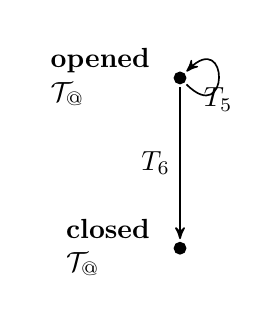
\begin{tikzpicture}[modal]
    \node[point] (opened) [label=left:{$\begin{array}{l}\mathbf{opened}\\ \mathcal{T}_@\end{array}$}] {};
     \node[point](closed) [below=of opened, label=180:{$\begin{array}{l}\mathbf{closed}\\\mathcal{T}_@  
    \end{array}$}] {};
    \path[->] (opened) edge[reflexive right,out=-45,in=45,looseness=18] node[below] {$T_5$} (opened);
      \path[->] (opened) edge node[left] {$T_6$} (closed);
\end{tikzpicture}
   % \caption{Caption}
    \label{fig:enter-label}
    \end{figure}
\end{columns}
\begin{itemize}
    \item More than just relating \textbf{STS}es in representation invariants per state.
    \item Bisimilar states can have different representation invariants.
    \end{itemize}
    \begin{alertblock}{Proof Indistinguishability}
        Knowing the proof of a client against the right (target STS conventionally $\pi'$)  \emph{enables} deducing the proof against the bisimilar on the left (source STS conventionally $\pi$).
    \end{alertblock}   
\end{frame}
\begin{frame}{A Quick Tour on \textbf{STS} Assertions}\scriptsize
\begin{itemize}
    \item Invariants $\fbox{$\varphi$}^{\gamma}_{\pi}$,  client capability $\ownGhost{\gamma}{s;\mathsf{T}}$
\end{itemize}
\begin{figure}
\centering
\scriptsize
\[
\begin{array}{l}
 \inferrule[STSAlloc]{ }{
    \varphi(s) \vs \exists \gamma \ldotp \fbox{$\varphi$}^{\gamma}_{\pi} \ast \ownGhost{\gamma}{s;\mathsf{AllTokens}\setminus\mathcal{T}(s)}
}\\
 \inferrule[STSOpen]{ }{
 \fbox{$\varphi$}^{\gamma}_{\pi} \ast \ownGhost{\gamma}{s;\mathsf{T}} \vs (\exists \; s' \ldotp \ulcorner  (\mathsf{s}0, \mathsf{T}) \overset{\mathsf{rely}^{*}}{\sqsubseteq}_{\pi} (\mathsf{s}',\mathsf{T}) \urcorner \ast \varphi(s) \ast \forall \mathsf{sl}', \;\mathsf{T}' \ldotp
      \ulcorner (\mathsf{s'}, \mathsf{T}) \overset{\mathsf{guar.}^{*}}{\sqsubseteq}_{\pi} (\mathsf{sl}', \mathsf{T}') \urcorner \ast \varphi(\mathsf{sl}') \vs \ownGhost{\gamma}{\mathsf{sl};\mathsf{T}'} )
 } \\
 \inferrule[UpdIsl]{
        \alpha~\textrm{physically atomic}\\
        \forall s_0 \;\ldotp  \;((s;\mathsf{T})\;\overset{\mathsf{rely}^{*}}{\sqsubseteq}_\pi\;( s_0;\mathsf{T}))\; \vdash
        \triple{ \varphi(s_0)\ast P }{\alpha}{ \exists s' \;, \;\mathsf{T}'\;\ldotp \; (s_0;\mathsf{T})\; \overset{\mathsf{guar}^{*}}{\sqsubseteq}_\pi \;(s';\mathsf{T}') \ast 
        \varphi(s')\ast Q}
    }{
      \fbox{$\varphi$}^{\gamma}_{\pi} \vdash
      \triple{ \ownGhost{\gamma}{s;\mathsf{T}} \ast P }
            {\alpha}
        { \exists \; s', \mathsf{T}' \ldotp \ownGhost{\gamma}{s';\mathsf{T}'} \ast Q }
    }
 \end{array}
\]
\vspace{-1em}
\caption{Iris STS Library ~\cite{Jung2015Iris} simplified with \textsf{later modality} and \textsf{invariant masks} omitted}
  \label{fig:stslib}
\end{figure}
\end{frame}
\section{Logic}
\subsection{Iris \textbf{STS} Library}
\begin{frame}{Decomposing Bisimilarity in \textbf{STS}es}\scriptsize
\begin{columns}
\column{0.4\textwidth}
The bisimulation ($\mathcal{M}(\pi,\pi',\varphi,\varphi',s,\mathsf{T},\mathsf{U})$) between two state machines, $\pi$ and $\pi'$ is composed of 
\begin{itemize}
\item The source STS -- $\pi$
\item The target STS -- $\pi'$
\item The source STS's state interpretation function -- $\varphi$
\item The target STS's state interpretation function -- $\varphi'$
    \item Token Embedding -- $\epsilon_{\mathcal{S}} : \;\; \mathcal{S}(\pi) \mapsto \mathcal{S}(\pi')$
    \item State Embedding -- $\epsilon_{\mathcal{T}} :\;\;  \mathcal{T}(\pi) \mapsto \mathcal{T}(\pi')$
    \item The Law of Rely 
    \item The Law of Guarantee
    \item The Law of Tolerance
    \item The state of source STS from which bisimulation is considered against any client interference with the token set $T$
\end{itemize}
\column{0.59\textwidth}
\begin{alertblock}{Proof Translation}
     Obtain a proof rule utilizing the bisimulation to translate proofs between bisimilar state machines!
\end{alertblock}
\end{columns}
\end{frame}
\subsection{Understanding Bisimulations}

\begin{frame}{Embeddings for Tokens and States}\scriptsize
\begin{columns}[c]
\column{0.4\textwidth}
\begin{figure}
    \centering
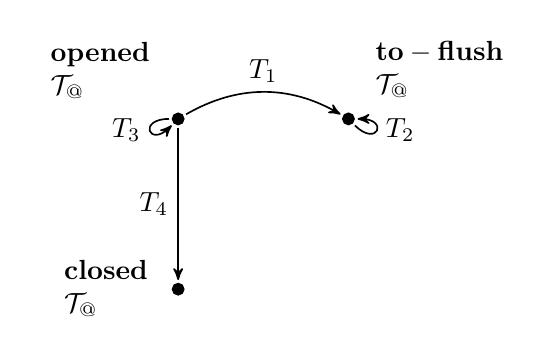
\begin{tikzpicture}[modal]
    \node[point] (to-flush) [label=135:{$\begin{array}{l}\mathbf{opened} \\ \mathcal{T}_@\end{array}$}] {};
    \node[point] (opened) [right=of to-flush, label=60:{$\begin{array}{l}\mathbf{to-flush}\\\mathcal{T}_@ 
    \end{array}$}] {};
    \node[point](closed) [below=of to-flush, label=180:{$\begin{array}{l}\mathbf{closed}\\\mathcal{T}_@  
    \end{array}$}] {};
    \path[->] (to-flush) edge[bend left] node[above]{$T_1$} (opened);
    \path[->] (opened) edge[reflexive right,out=-45,in=0,looseness=18] node[right] {$T_2$} (opened);
    \path[->] (to-flush) edge[reflexive left,out=180,in=225,looseness=18] node[left] {$T_3$} (to-flush);
     \path[->] (to-flush) edge node[left] {$T_4$} (closed);
\end{tikzpicture}
 %   \caption{Caption}
    \label{fig:enter-label}
\end{figure}
\column{.2\textwidth}
\begin{figure}
    \centering
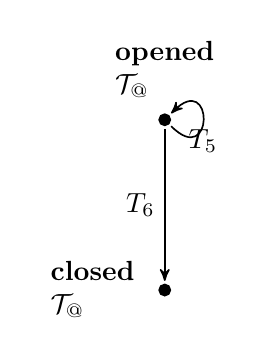
\begin{tikzpicture}[modal]
    \node[point] (opened) [label=above:{$\begin{array}{l}\mathbf{opened}\\ \mathcal{T}_@\end{array}$}] {};
     \node[point](closed) [below=of opened, label=180:{$\begin{array}{l}\mathbf{closed}\\\mathcal{T}_@ 
    \end{array}$}] {};
    \path[->] (opened) edge[reflexive right,out=-45,in=45,looseness=18] node[below] {$T_5$} (opened);
      \path[->] (opened) edge node[left] {$T_6$} (closed);
    
\end{tikzpicture}
  %  \caption{Caption}
    \label{fig:enter-label}
    \end{figure}
\column{0.39\textwidth}
\begin{itemize}
    \item How to impose \emph{indistinguishability} of behavior observed on \emph{bisimilar} states
    \item How to impose \emph{indistinguishability} over the steps taken between \emph{bisimilar} states
\end{itemize}
\end{columns}
\end{frame}
\begin{frame}{Embeddings for Tokens }\scriptsize
\begin{columns}[c]
\column{0.4\textwidth}
\begin{figure}
    \centering
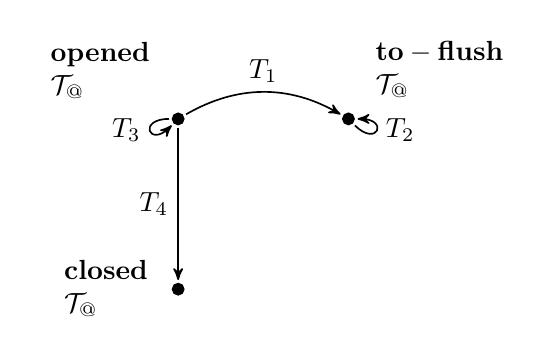
\begin{tikzpicture}[modal]
    \node[point] (to-flush) [label=135:{$\begin{array}{l}\mathbf{opened} \\ \mathcal{T}_@\end{array}$}] {};
    \node[point] (opened) [right=of to-flush, label=60:{$\begin{array}{l}\mathbf{to-flush}\\\mathcal{T}_@ 
    \end{array}$}] {};
    \node[point](closed) [below=of to-flush, label=180:{$\begin{array}{l}\mathbf{closed}\\\mathcal{T}_@  
    \end{array}$}] {};
    \path[->] (to-flush) edge[bend left] node[above]{$T_1$} (opened);
    \path[->] (opened) edge[reflexive right,out=-45,in=0,looseness=18] node[right] {$T_2$} (opened);
    \path[->] (to-flush) edge[reflexive left,out=180,in=225,looseness=18] node[left] {$T_3$} (to-flush);
     \path[->] (to-flush) edge node[left] {$T_4$} (closed);
\end{tikzpicture}
 %   \caption{Caption}
    \label{fig:enter-label}
\end{figure}
\column{.2\textwidth}
\begin{figure}
    \centering
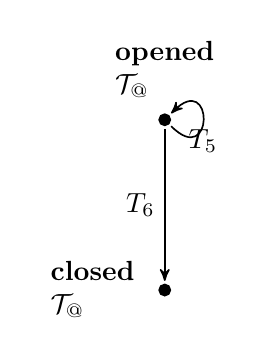
\begin{tikzpicture}[modal]
    \node[point] (opened) [label=above:{$\begin{array}{l}\mathbf{opened}\\ \mathcal{T}_@\end{array}$}] {};
     \node[point](closed) [below=of opened, label=180:{$\begin{array}{l}\mathbf{closed}\\\mathcal{T}_@ 
    \end{array}$}] {};
    \path[->] (opened) edge[reflexive right,out=-45,in=45,looseness=18] node[below] {$T_5$} (opened);
      \path[->] (opened) edge node[left] {$T_6$} (closed);
    
\end{tikzpicture}
  %  \caption{Caption}
    \label{fig:enter-label}
    \end{figure}
\column{0.39\textwidth}
\begin{itemize}
    \item Make \emph{token exchange} align with \emph{indistinguishability}: Embedding tokens (lifted $\epsilon_{\overline{\mathcal{T}}}$) $T_1$, $T_3$, and $T_2$ to $T_5$, and $T_4$ to $T_6$
\end{itemize}
\end{columns}
\end{frame}
\begin{frame}{Embeddings for State}\scriptsize
\begin{columns}[c]
\column{0.4\textwidth}
\begin{figure}
    \centering
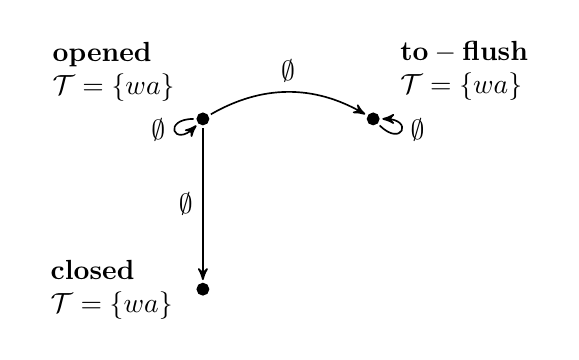
\begin{tikzpicture}[modal]
    \node[point] (to-flush) [label=135:{$\begin{array}{l}\mathbf{opened} \\ \mathcal{T}=\{wa\}\end{array}$}] {};
    \node[point] (opened) [right=of to-flush, label=60:{$\begin{array}{l}\mathbf{to-flush}\\\mathcal{T} = \{wa\} 
    \end{array}$}] {};
    \node[point](closed) [below=of to-flush, label=180:{$\begin{array}{l}\mathbf{closed}\\\mathcal{T} = \{wa\} 
    \end{array}$}] {};
    \path[->] (to-flush) edge[bend left] node[above]{$\emptyset$} (opened);
    \path[->] (opened) edge[reflexive right,out=-45,in=0,looseness=18] node[right] {$\emptyset$} (opened);
    \path[->] (to-flush) edge[reflexive left,out=180,in=225,looseness=18] node[left] {$\emptyset$} (to-flush);
     \path[->] (to-flush) edge node[left] {$\emptyset$} (closed);
\end{tikzpicture}
  %  \caption{Caption}
    \label{fig:enter-label}
\end{figure}
\column{.2\textwidth}
\begin{figure}
    \centering
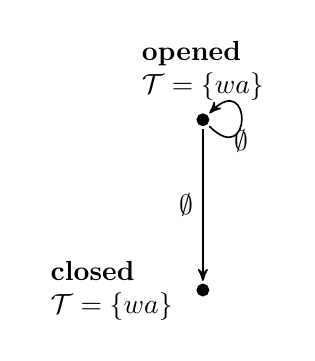
\begin{tikzpicture}[modal]
    \node[point] (opened) [label=above:{$\begin{array}{l}\mathbf{opened}\\ \mathcal{T}=\{wa\}\end{array}$}] {};
     \node[point](closed) [below=of opened, label=180:{$\begin{array}{l}\mathbf{closed}\\\mathcal{T} = \{wa\} 
    \end{array}$}] {};
    \path[->] (opened) edge[reflexive right,out=-45,in=45,looseness=18] node[below] {$\emptyset$} (opened);
      \path[->] (opened) edge node[left] {$\emptyset$} (closed);
\end{tikzpicture}
%    \caption{Caption}
    \label{fig:enter-label}
    \end{figure}
    \column{0.39\textwidth}
    \begin{itemize}
        \item Setting client interference aside, we would consider \textsf{opened} and \textsf{flushed} of the left state machine to be \emph{bisimilar} to \textsf{opened} of the right state machine
    \end{itemize}
\end{columns}
\end{frame}
\begin{frame}{A Quick Tour on the Represention of Laws - 1}\scriptsize
    \begin{figure}
\centering
 \scriptsize 
\tikzset {_n2izikt79/.code = {\pgfsetadditionalshadetransform{ \pgftransformshift{\pgfpoint{0 bp } { 0 bp }  }  \pgftransformrotate{0 }  \pgftransformscale{2 }  }}}
\pgfdeclarehorizontalshading{_s7jexb44p}{150bp}{rgb(0bp)=(0.27,0.28,0.3);
rgb(37.5bp)=(0.27,0.28,0.3);
rgb(62.5bp)=(0,0,0);
rgb(100bp)=(0,0,0)}

% Gradient Info
  
\tikzset {_9fn8o2jyc/.code = {\pgfsetadditionalshadetransform{ \pgftransformshift{\pgfpoint{0 bp } { 0 bp }  }  \pgftransformrotate{0 }  \pgftransformscale{2 }  }}}
\pgfdeclarehorizontalshading{_ua9wrsy9c}{150bp}{rgb(0bp)=(0.27,0.28,0.3);
rgb(37.5bp)=(0.27,0.28,0.3);
rgb(62.5bp)=(0,0,0);
rgb(100bp)=(0,0,0)}
\tikzset{every picture/.style={line width=0.75pt}} %set default line width to 0.75pt        

\begin{tikzpicture}[x=0.75pt,y=0.75pt,yscale=-0.75,xscale=0.75]
%uncomment if require: \path (0,1468); %set diagram left start at 0, and has height of 1468

%Flowchart: Terminator [id:dp6822294556237123] 
\draw   (85.4,178) -- (197.6,178) .. controls (212.18,178) and (224,188.52) .. (224,201.5) .. controls (224,214.48) and (212.18,225) .. (197.6,225) -- (85.4,225) .. controls (70.82,225) and (59,214.48) .. (59,201.5) .. controls (59,188.52) and (70.82,178) .. (85.4,178) -- cycle ;
%Flowchart: Terminator [id:dp14665687884367173] 
\draw   (84.56,253) -- (197.44,253) .. controls (212.11,253) and (224,263.52) .. (224,276.5) .. controls (224,289.48) and (212.11,300) .. (197.44,300) -- (84.56,300) .. controls (69.89,300) and (58,289.48) .. (58,276.5) .. controls (58,263.52) and (69.89,253) .. (84.56,253) -- cycle ;
%Shape: Circle [id:dp8811061876983324] 
\draw  [fill={rgb, 255:red, 0; green, 0; blue, 0 }  ,fill opacity=1 ] (183.95,61.38) .. controls (184.3,63.56) and (182.81,65.61) .. (180.62,65.95) .. controls (178.44,66.3) and (176.39,64.81) .. (176.05,62.62) .. controls (175.7,60.44) and (177.19,58.39) .. (179.38,58.05) .. controls (181.56,57.7) and (183.61,59.19) .. (183.95,61.38) -- cycle ;
%Shape: Circle [id:dp17791788002299502] 
\draw  [fill={rgb, 255:red, 0; green, 0; blue, 0 }  ,fill opacity=1 ] (102.45,61.38) .. controls (102.8,63.56) and (101.31,65.61) .. (99.12,65.95) .. controls (96.94,66.3) and (94.89,64.81) .. (94.55,62.62) .. controls (94.2,60.44) and (95.69,58.39) .. (97.88,58.05) .. controls (100.06,57.7) and (102.11,59.19) .. (102.45,61.38) -- cycle ;
%Flowchart: Terminator [id:dp5184102396793047] 
\draw   (83.2,26) -- (198.8,26) .. controls (213.82,26) and (226,52.42) .. (226,85) .. controls (226,117.58) and (213.82,144) .. (198.8,144) -- (83.2,144) .. controls (68.18,144) and (56,117.58) .. (56,85) .. controls (56,52.42) and (68.18,26) .. (83.2,26) -- cycle ;
%Curve Lines [id:da25462232906323323] 
\draw    (108,72) .. controls (123.68,84.74) and (150.88,85.96) .. (175.5,72.82) ;
\draw [shift={(177,72)}, rotate = 150.75] [color={rgb, 255:red, 0; green, 0; blue, 0 }  ][line width=0.75]    (10.93,-3.29) .. controls (6.95,-1.4) and (3.31,-0.3) .. (0,0) .. controls (3.31,0.3) and (6.95,1.4) .. (10.93,3.29)   ;
%Flowchart: Terminator [id:dp5285972700896346] 
\draw   (295.28,29) -- (436.72,29) .. controls (455.1,29) and (470,51.39) .. (470,79) .. controls (470,106.61) and (455.1,129) .. (436.72,129) -- (295.28,129) .. controls (276.9,129) and (262,106.61) .. (262,79) .. controls (262,51.39) and (276.9,29) .. (295.28,29) -- cycle ;
%Shape: Circle [id:dp41692609213252685] 
\draw  [fill={rgb, 255:red, 0; green, 0; blue, 0 }  ,fill opacity=1 ] (317.5,96) .. controls (317.84,98.18) and (316.35,100.23) .. (314.17,100.57) .. controls (311.99,100.92) and (309.94,99.43) .. (309.6,97.25) .. controls (309.25,95.06) and (310.74,93.02) .. (312.93,92.67) .. controls (315.11,92.33) and (317.16,93.82) .. (317.5,96) -- cycle ;
%Curve Lines [id:da9154734647409228] 
\draw    (319,96) .. controls (365.04,89.07) and (357.16,88.02) .. (410.37,98.67) ;
\draw [shift={(412,99)}, rotate = 191.31] [color={rgb, 255:red, 0; green, 0; blue, 0 }  ][line width=0.75]    (10.93,-3.29) .. controls (6.95,-1.4) and (3.31,-0.3) .. (0,0) .. controls (3.31,0.3) and (6.95,1.4) .. (10.93,3.29)   ;
%Shape: Circle [id:dp47950732435753207] 
\draw  [fill={rgb, 255:red, 0; green, 0; blue, 0 }  ,fill opacity=1 ] (422,96) .. controls (422.34,98.18) and (420.85,100.23) .. (418.67,100.57) .. controls (416.49,100.92) and (414.44,99.43) .. (414.1,97.25) .. controls (413.75,95.06) and (415.24,93.02) .. (417.43,92.67) .. controls (419.61,92.33) and (421.66,93.82) .. (422,96) -- cycle ;
%Curve Lines [id:da7701997446029554] 
\draw [color={rgb, 255:red, 0; green, 0; blue, 0 }  ,draw opacity=1 ]   (441.66,271) .. controls (362,271) and (366.44,271) .. (345.72,271) ;
\draw [shift={(345.72,271)}, rotate = 360] [color={rgb, 255:red, 0; green, 0; blue, 0 }  ,draw opacity=1 ][line width=0.75]    (0,5.59) -- (0,-5.59)(-5.03,5.59) -- (-5.03,-5.59)   ;
\draw [shift={(441.66,271)}, rotate = 180] [color={rgb, 255:red, 0; green, 0; blue, 0 }  ,draw opacity=1 ][line width=0.75]    (0,5.59) -- (0,-5.59)(-5.03,5.59) -- (-5.03,-5.59)   ;
%Shape: Circle [id:dp7968250836601951] 
\draw  [fill={rgb, 255:red, 0; green, 0; blue, 0 }  ,fill opacity=1 ] (331.5,270) .. controls (331.84,272.18) and (330.35,274.23) .. (328.17,274.57) .. controls (325.99,274.92) and (323.94,273.43) .. (323.6,271.25) .. controls (323.25,269.06) and (324.74,267.02) .. (326.93,266.67) .. controls (329.11,266.33) and (331.16,267.82) .. (331.5,270) -- cycle ;
%Shape: Circle [id:dp7887383741800589] 
\draw  [fill={rgb, 255:red, 0; green, 0; blue, 0 }  ,fill opacity=1 ] (462.5,270) .. controls (462.84,272.18) and (461.35,274.23) .. (459.17,274.57) .. controls (456.99,274.92) and (454.94,273.43) .. (454.6,271.25) .. controls (454.25,269.06) and (455.74,267.02) .. (457.93,266.67) .. controls (460.11,266.33) and (462.16,267.82) .. (462.5,270) -- cycle ;
%Shape: Circle [id:dp34594755012909295] 
\draw  [fill={rgb, 255:red, 0; green, 0; blue, 0 }  ,fill opacity=1 ] (319.05,157.31) .. controls (319.39,159.49) and (317.9,161.54) .. (315.72,161.89) .. controls (313.54,162.23) and (311.49,160.74) .. (311.15,158.56) .. controls (310.8,156.37) and (312.29,154.33) .. (314.47,153.98) .. controls (316.66,153.64) and (318.7,155.13) .. (319.05,157.31) -- cycle ;
%Straight Lines [id:da012219441875116921] 
\draw  [dash pattern={on 0.75pt off 0.75pt}]  (663.93,126.67) .. controls (662.29,124.98) and (662.32,123.31) .. (664.01,121.67) .. controls (665.7,120.03) and (665.73,118.36) .. (664.1,116.67) .. controls (662.46,114.98) and (662.49,113.31) .. (664.18,111.67) .. controls (665.87,110.03) and (665.9,108.36) .. (664.27,106.67) .. controls (662.63,104.98) and (662.66,103.31) .. (664.35,101.68) .. controls (666.04,100.04) and (666.07,98.37) .. (664.44,96.68) .. controls (662.81,94.99) and (662.84,93.32) .. (664.53,91.68) .. controls (666.22,90.04) and (666.25,88.37) .. (664.61,86.68) .. controls (662.98,84.99) and (663.01,83.32) .. (664.7,81.68) .. controls (666.39,80.04) and (666.42,78.37) .. (664.78,76.68) .. controls (663.15,74.99) and (663.18,73.32) .. (664.87,71.68) .. controls (666.56,70.04) and (666.59,68.37) .. (664.95,66.68) -- (665,64) -- (665,64) ;
%Curve Lines [id:da14562814262188062] 
\draw [color={rgb, 255:red, 0; green, 0; blue, 0 }  ,draw opacity=1 ]   (647,279.49) .. controls (647,266.67) and (647,259.01) .. (647,227.17) ;
\draw [shift={(647,227.17)}, rotate = 90] [color={rgb, 255:red, 0; green, 0; blue, 0 }  ,draw opacity=1 ][line width=0.75]    (0,5.59) -- (0,-5.59)(-5.03,5.59) -- (-5.03,-5.59)   ;
\draw [shift={(647,279.49)}, rotate = 270] [color={rgb, 255:red, 0; green, 0; blue, 0 }  ,draw opacity=1 ][line width=0.75]    (0,5.59) -- (0,-5.59)(-5.03,5.59) -- (-5.03,-5.59)   ;
%Flowchart: Terminator [id:dp8041546240843622] 
\draw   (289.08,244) -- (348.92,244) .. controls (356.7,244) and (363,257.21) .. (363,273.5) .. controls (363,289.79) and (356.7,303) .. (348.92,303) -- (289.08,303) .. controls (281.3,303) and (275,289.79) .. (275,273.5) .. controls (275,257.21) and (281.3,244) .. (289.08,244) -- cycle ;
%Flowchart: Terminator [id:dp42463689879734434] 
\draw   (438.08,244) -- (497.92,244) .. controls (505.7,244) and (512,257.21) .. (512,273.5) .. controls (512,289.79) and (505.7,303) .. (497.92,303) -- (438.08,303) .. controls (430.3,303) and (424,289.79) .. (424,273.5) .. controls (424,257.21) and (430.3,244) .. (438.08,244) -- cycle ;
%Shape: Circle [id:dp7924872921588482] 
\draw  [fill={rgb, 255:red, 0; green, 0; blue, 0 }  ,fill opacity=1 ] (557.45,124.38) .. controls (557.8,126.56) and (556.31,128.61) .. (554.12,128.95) .. controls (551.94,129.3) and (549.89,127.81) .. (549.55,125.62) .. controls (549.2,123.44) and (550.69,121.39) .. (552.88,121.05) .. controls (555.06,120.7) and (557.11,122.19) .. (557.45,124.38) -- cycle ;
%Straight Lines [id:da3112366150868817] 
\draw    (553,134.5) -- (553,201.5) ;
\draw [shift={(553,201.5)}, rotate = 270] [color={rgb, 255:red, 0; green, 0; blue, 0 }  ][line width=0.75]    (0,5.59) -- (0,-5.59)(17.64,-4.9) .. controls (13.66,-2.3) and (10.02,-0.67) .. (6.71,0) .. controls (10.02,0.67) and (13.66,2.3) .. (17.64,4.9)(10.93,-4.9) .. controls (6.95,-2.3) and (3.31,-0.67) .. (0,0) .. controls (3.31,0.67) and (6.95,2.3) .. (10.93,4.9)   ;
\draw [shift={(553,134.5)}, rotate = 90] [color={rgb, 255:red, 0; green, 0; blue, 0 }  ][line width=0.75]    (0,5.59) -- (0,-5.59)(17.64,-4.9) .. controls (13.66,-2.3) and (10.02,-0.67) .. (6.71,0) .. controls (10.02,0.67) and (13.66,2.3) .. (17.64,4.9)(10.93,-4.9) .. controls (6.95,-2.3) and (3.31,-0.67) .. (0,0) .. controls (3.31,0.67) and (6.95,2.3) .. (10.93,4.9)   ;
%Flowchart: Terminator [id:dp8577436650377137] 
\draw   (507.44,103) -- (581.56,103) .. controls (591.19,103) and (599,114.05) .. (599,127.69) .. controls (599,141.32) and (591.19,152.38) .. (581.56,152.38) -- (507.44,152.38) .. controls (497.81,152.38) and (490,141.32) .. (490,127.69) .. controls (490,114.05) and (497.81,103) .. (507.44,103) -- cycle ;
%Flowchart: Terminator [id:dp5790671492690609] 
\draw   (648.28,20) -- (738.72,20) .. controls (750.47,20) and (760,30.97) .. (760,44.5) .. controls (760,58.03) and (750.47,69) .. (738.72,69) -- (648.28,69) .. controls (636.53,69) and (627,58.03) .. (627,44.5) .. controls (627,30.97) and (636.53,20) .. (648.28,20) -- cycle ;
%Straight Lines [id:da557442761280283] 
\draw  [dash pattern={on 0.75pt off 0.75pt}]  (720.5,127) .. controls (718.85,125.32) and (718.86,123.65) .. (720.54,122) .. controls (722.22,120.35) and (722.23,118.68) .. (720.58,117) .. controls (718.93,115.32) and (718.94,113.65) .. (720.62,112) .. controls (722.3,110.35) and (722.31,108.68) .. (720.66,107) .. controls (719.01,105.33) and (719.02,103.66) .. (720.69,102) .. controls (722.37,100.35) and (722.38,98.68) .. (720.73,97) .. controls (719.08,95.32) and (719.09,93.65) .. (720.77,92) .. controls (722.45,90.35) and (722.46,88.68) .. (720.81,87) .. controls (719.16,85.32) and (719.17,83.65) .. (720.85,82) .. controls (722.53,80.35) and (722.54,78.68) .. (720.89,77) .. controls (719.24,75.32) and (719.25,73.65) .. (720.93,72) .. controls (722.61,70.35) and (722.62,68.68) .. (720.97,67) -- (721,62.5) -- (721,62.5) ;
%Flowchart: Terminator [id:dp13592197897622604] 
\draw   (648.28,117) -- (738.72,117) .. controls (750.47,117) and (760,128.08) .. (760,141.75) .. controls (760,155.42) and (750.47,166.5) .. (738.72,166.5) -- (648.28,166.5) .. controls (636.53,166.5) and (627,155.42) .. (627,141.75) .. controls (627,128.08) and (636.53,117) .. (648.28,117) -- cycle ;
%Shape: Circle [id:dp7995856620691222] 
\draw  [fill={rgb, 255:red, 0; green, 0; blue, 0 }  ,fill opacity=1 ] (668.5,130) .. controls (668.84,132.18) and (667.35,134.23) .. (665.17,134.57) .. controls (662.99,134.92) and (660.94,133.43) .. (660.6,131.25) .. controls (660.25,129.06) and (661.74,127.02) .. (663.93,126.67) .. controls (666.11,126.33) and (668.16,127.82) .. (668.5,130) -- cycle ;
%Shape: Circle [id:dp032836164451744976] 
\draw  [fill={rgb, 255:red, 0; green, 0; blue, 0 }  ,fill opacity=1 ] (725.07,130.33) .. controls (725.42,132.51) and (723.93,134.56) .. (721.75,134.9) .. controls (719.56,135.25) and (717.52,133.76) .. (717.17,131.57) .. controls (716.83,129.39) and (718.32,127.34) .. (720.5,127) .. controls (722.68,126.66) and (724.73,128.15) .. (725.07,130.33) -- cycle ;
%Flowchart: Terminator [id:dp2731298339516455] 
\draw   (634.36,192) -- (733.64,192) .. controls (746.54,192) and (757,200.66) .. (757,211.35) .. controls (757,222.04) and (746.54,230.71) .. (733.64,230.71) -- (634.36,230.71) .. controls (621.46,230.71) and (611,222.04) .. (611,211.35) .. controls (611,200.66) and (621.46,192) .. (634.36,192) -- cycle ;
%Flowchart: Terminator [id:dp42354682334110194] 
\draw   (608.48,276.5) -- (729.52,276.5) .. controls (745.25,276.5) and (758,286.01) .. (758,297.75) .. controls (758,309.49) and (745.25,319) .. (729.52,319) -- (608.48,319) .. controls (592.75,319) and (580,309.49) .. (580,297.75) .. controls (580,286.01) and (592.75,276.5) .. (608.48,276.5) -- cycle ;
%Shape: Circle [id:dp07103980451569458] 
\draw  [fill={rgb, 255:red, 0; green, 0; blue, 0 }  ,fill opacity=1 ] (651.5,293.71) .. controls (651.84,295.89) and (650.35,297.94) .. (648.17,298.28) .. controls (645.99,298.62) and (643.94,297.13) .. (643.6,294.95) .. controls (643.25,292.77) and (644.74,290.72) .. (646.93,290.38) .. controls (649.11,290.03) and (651.16,291.52) .. (651.5,293.71) -- cycle ;
%Shape: Circle [id:dp21119276076705584] 
\draw  [fill={rgb, 255:red, 0; green, 0; blue, 0 }  ,fill opacity=1 ] (726.07,293.03) .. controls (726.42,295.22) and (724.93,297.26) .. (722.75,297.61) .. controls (720.56,297.95) and (718.52,296.46) .. (718.17,294.28) .. controls (717.83,292.1) and (719.32,290.05) .. (721.5,289.71) .. controls (723.68,289.36) and (725.73,290.85) .. (726.07,293.03) -- cycle ;
%Curve Lines [id:da8088255036703353] 
\draw [color={rgb, 255:red, 0; green, 0; blue, 0 }  ,draw opacity=1 ]   (726.38,280.66) .. controls (742.58,260.19) and (738.77,229.36) .. (651.07,222.78) ;
\draw [shift={(651.07,222.78)}, rotate = 3.69] [color={rgb, 255:red, 0; green, 0; blue, 0 }  ,draw opacity=1 ][line width=0.75]    (0,5.59) -- (0,-5.59)(-5.03,5.59) -- (-5.03,-5.59)   ;
\draw [shift={(726.38,280.66)}, rotate = 314.29] [color={rgb, 255:red, 0; green, 0; blue, 0 }  ,draw opacity=1 ][line width=0.75]    (0,5.59) -- (0,-5.59)(-5.03,5.59) -- (-5.03,-5.59)   ;
%Shape: Circle [id:dp1496083197283049] 
\draw  [fill={rgb, 255:red, 0; green, 0; blue, 0 }  ,fill opacity=1 ] (668.5,56) .. controls (668.84,58.18) and (667.35,60.23) .. (665.17,60.57) .. controls (662.99,60.92) and (660.94,59.43) .. (660.6,57.25) .. controls (660.25,55.06) and (661.74,53.02) .. (663.93,52.67) .. controls (666.11,52.33) and (668.16,53.82) .. (668.5,56) -- cycle ;
%Shape: Circle [id:dp5013810079001233] 
\draw  [fill={rgb, 255:red, 0; green, 0; blue, 0 }  ,fill opacity=1 ] (723.5,56) .. controls (723.84,58.18) and (722.35,60.23) .. (720.17,60.57) .. controls (717.99,60.92) and (715.94,59.43) .. (715.6,57.25) .. controls (715.25,55.06) and (716.74,53.02) .. (718.93,52.67) .. controls (721.11,52.33) and (723.16,53.82) .. (723.5,56) -- cycle ;
%Shape: Circle [id:dp6827215473552395] 
\draw  [fill={rgb, 255:red, 0; green, 0; blue, 0 }  ,fill opacity=1 ] (650.5,211.71) .. controls (650.84,213.89) and (649.35,215.94) .. (647.17,216.28) .. controls (644.99,216.62) and (642.94,215.13) .. (642.6,212.95) .. controls (642.25,210.77) and (643.74,208.72) .. (645.93,208.38) .. controls (648.11,208.03) and (650.16,209.52) .. (650.5,211.71) -- cycle ;
%Shape: Regular Polygon [id:dp34726153491144385] 
\path  [shading=_s7jexb44p,_n2izikt79] (365.5,152.75) -- (356.63,168.12) -- (338.88,168.12) -- (330,152.75) -- (338.88,137.38) -- (356.63,137.38) -- cycle ; % for fading 
 \draw   (365.5,152.75) -- (356.63,168.12) -- (338.88,168.12) -- (330,152.75) -- (338.88,137.38) -- (356.63,137.38) -- cycle ; % for border 

%Shape: Regular Polygon [id:dp504474767758126] 
\path  [shading=_ua9wrsy9c,_9fn8o2jyc] (418.75,152.75) -- (413.19,166.19) -- (399.75,171.75) -- (386.31,166.19) -- (380.75,152.75) -- (386.31,139.31) -- (399.75,133.75) -- (413.19,139.31) -- cycle ; % for fading 
 \draw   (418.75,152.75) -- (413.19,166.19) -- (399.75,171.75) -- (386.31,166.19) -- (380.75,152.75) -- (386.31,139.31) -- (399.75,133.75) -- (413.19,139.31) -- cycle ; % for border 

%Shape: Regular Polygon [id:dp2404141286640462] 
\draw  [fill={rgb, 255:red, 255; green, 255; blue, 255 }  ,fill opacity=1 ] (336.13,198.38) -- (330.63,211.63) -- (317.38,217.13) -- (304.12,211.63) -- (298.63,198.38) -- (304.12,185.12) -- (317.38,179.63) -- (330.63,185.12) -- cycle ;
%Shape: Regular Polygon [id:dp4573777592505157] 
\draw  [color={rgb, 255:red, 0; green, 0; blue, 0 }  ,draw opacity=1 ][fill={rgb, 255:red, 255; green, 255; blue, 255 }  ,fill opacity=1 ] (391,198.38) -- (381.19,215.37) -- (361.56,215.37) -- (351.75,198.38) -- (361.56,181.38) -- (381.19,181.38) -- cycle ;
%Flowchart: Terminator [id:dp5008847585485463] 
\draw   (510.44,25) -- (584.56,25) .. controls (594.19,25) and (602,36.05) .. (602,49.69) .. controls (602,63.32) and (594.19,74.38) .. (584.56,74.38) -- (510.44,74.38) .. controls (500.81,74.38) and (493,63.32) .. (493,49.69) .. controls (493,36.05) and (500.81,25) .. (510.44,25) -- cycle ;
%Shape: Circle [id:dp48786584141259204] 
\draw  [fill={rgb, 255:red, 0; green, 0; blue, 0 }  ,fill opacity=1 ] (557.45,48.38) .. controls (557.8,50.56) and (556.31,52.61) .. (554.12,52.95) .. controls (551.94,53.3) and (549.89,51.81) .. (549.55,49.62) .. controls (549.2,47.44) and (550.69,45.39) .. (552.88,45.05) .. controls (555.06,44.7) and (557.11,46.19) .. (557.45,48.38) -- cycle ;
%Straight Lines [id:da3732059402424506] 
\draw  [dash pattern={on 0.75pt off 0.75pt}]  (552.88,119.05) .. controls (551.24,117.36) and (551.27,115.69) .. (552.96,114.05) .. controls (554.65,112.41) and (554.68,110.74) .. (553.05,109.05) .. controls (551.41,107.36) and (551.44,105.69) .. (553.13,104.05) .. controls (554.82,102.41) and (554.85,100.74) .. (553.22,99.05) .. controls (551.59,97.36) and (551.62,95.69) .. (553.31,94.05) .. controls (555,92.41) and (555.03,90.74) .. (553.39,89.05) .. controls (551.76,87.36) and (551.79,85.69) .. (553.48,84.05) .. controls (555.17,82.41) and (555.2,80.74) .. (553.56,79.05) .. controls (551.93,77.36) and (551.96,75.69) .. (553.65,74.06) .. controls (555.34,72.42) and (555.37,70.75) .. (553.73,69.06) .. controls (552.1,67.37) and (552.13,65.7) .. (553.82,64.06) .. controls (555.51,62.42) and (555.54,60.75) .. (553.91,59.06) -- (553.95,56.38) -- (553.95,56.38) ;

% Text Nodex
\draw (74,184.8) node [anchor=north west][inner sep=0.75pt]  [font=\scriptsize] [align=left] {$\displaystyle \mathcal{T}( \pi )$};
% Text Node
\draw (173,184.31) node [anchor=north west][inner sep=0.75pt]  [font=\scriptsize] [align=left] {$\displaystyle \mathcal{T}( \pi ')$};
% Text Node
\draw (169,262) node [anchor=north west][inner sep=0.75pt]  [font=\scriptsize] [align=left] {$\displaystyle \mathcal{S}( \pi ')$};
% Text Node
\draw (74,262) node [anchor=north west][inner sep=0.75pt]  [font=\scriptsize] [align=left] {$\displaystyle \mathcal{S}( \pi )$};
% Text Node
\draw (162,116) node [anchor=north west][inner sep=0.75pt]  [font=\scriptsize] [align=left] {$\displaystyle \mathcal{S}( \pi ')$};
% Text Node
\draw (82,115) node [anchor=north west][inner sep=0.75pt]  [font=\scriptsize] [align=left] {$\displaystyle \mathcal{S}( \pi )$};
% Text Node
\draw (97,42) node    {$s$};
% Text Node
\draw (180,43) node    {$s'$};
% Text Node
\draw (140,95) node    {$\epsilon_{\mathcal{S}}$};
% Text Node
\draw (288,34) node [anchor=north west][inner sep=0.75pt]  [font=\scriptsize] [align=left] {$\displaystyle \mathcal{T}( \pi )$};
% Text Node
\draw (403,34) node [anchor=north west][inner sep=0.75pt]  [font=\scriptsize] [align=left] {$\displaystyle \mathcal{T}( \pi ')$};
% Text Node
\draw (301,98) node  [font=\scriptsize]  {$T$};
% Text Node
\draw (361,79) node  [font=\scriptsize]  {$\epsilon_{\overline{\mathcal{T}}}$};
% Text Node
\draw (435,96) node  [font=\scriptsize]  {$T'$};
% Text Node
\draw (329,286) node  [font=\scriptsize]  {$T$};
% Text Node
\draw (460,282) node    {$s$};
% Text Node
\draw (16,26) node [anchor=north west][inner sep=0.75pt]  [color={rgb, 255:red, 0; green, 0; blue, 0 }  ,opacity=1 ] [align=left] {1};
% Text Node
\draw (243,26) node [anchor=north west][inner sep=0.75pt]  [color={rgb, 255:red, 0; green, 0; blue, 0 }  ,opacity=1 ] [align=left] {2};
% Text Node
\draw (18,175) node [anchor=north west][inner sep=0.75pt]  [color={rgb, 255:red, 0; green, 0; blue, 0 }  ,opacity=1 ] [align=left] {3};
% Text Node
\draw (255,145) node [anchor=north west][inner sep=0.75pt]  [color={rgb, 255:red, 0; green, 0; blue, 0 }  ,opacity=1 ] [align=left] {4};
% Text Node
\draw (18,264) node [anchor=north west][inner sep=0.75pt]  [color={rgb, 255:red, 0; green, 0; blue, 0 }  ,opacity=1 ] [align=left] {6};
% Text Node
\draw (248,265) node [anchor=north west][inner sep=0.75pt]  [color={rgb, 255:red, 0; green, 0; blue, 0 }  ,opacity=1 ] [align=left] {11};
% Text Node
\draw (607,25) node [anchor=north west][inner sep=0.75pt]  [color={rgb, 255:red, 0; green, 0; blue, 0 }  ,opacity=1 ] [align=left] {7};
% Text Node
\draw (592,180) node [anchor=north west][inner sep=0.75pt]  [color={rgb, 255:red, 0; green, 0; blue, 0 }  ,opacity=1 ] [align=left] {8};
% Text Node
\draw  [color={rgb, 255:red, 255; green, 255; blue, 255 }  ,draw opacity=1 ][fill={rgb, 255:red, 255; green, 255; blue, 255 }  ,fill opacity=1 ]  (686, 87) circle [x radius= 9.9, y radius= 12.73]   ;
\draw (678,77) node [anchor=north west][inner sep=0.75pt]  [font=\scriptsize] [align=left] {$\overset{\mathsf{guar.}^{*}}{\sqsubseteq}_{\pi}$};
% Text Node
\draw  [color={rgb, 255:red, 255; green, 255; blue, 255 }  ,draw opacity=1 ][fill={rgb, 255:red, 255; green, 255; blue, 255 }  ,fill opacity=1 ]  (667.5, 251) circle [x radius= 9.19, y radius= 12.73]   ;
\draw (660,241) node [anchor=north west][inner sep=0.75pt]  [font=\scriptsize] [align=left] {$\overset{\mathsf{rely.}^{*}}{\sqsubseteq}_{\pi}$};
% Text Node
\draw (278,261.29) node [anchor=north west][inner sep=0.75pt]  [font=\scriptsize] [align=left] {$\displaystyle \mathcal{T}( \pi )$};
% Text Node
\draw (476,262) node [anchor=north west][inner sep=0.75pt]  [font=\scriptsize] [align=left] {$\displaystyle \mathcal{S}( \pi )$};
% Text Node
\draw (498,115) node [anchor=north west][inner sep=0.75pt]  [font=\scriptsize] [align=left] {$\displaystyle \mathcal{S}( \pi )$};
% Text Node
\draw (572,123) node    {$s$};
% Text Node
\draw (527,210) node [anchor=north west][inner sep=0.75pt]  [font=\scriptsize] [align=left] {$\mathsf{Inv}( s )$};
% Text Node
\draw (526,162) node [anchor=north west][inner sep=0.75pt]  [font=\scriptsize] [align=left] {$\displaystyle \varphi $};
% Text Node
\draw (474,23) node [anchor=north west][inner sep=0.75pt]  [color={rgb, 255:red, 0; green, 0; blue, 0 }  ,opacity=1 ] [align=left] {9};
% Text Node
\draw (650,23.29) node [anchor=north west][inner sep=0.75pt]  [font=\scriptsize] [align=left] {$\displaystyle \mathcal{T}( \pi )$};
% Text Node
\draw (705,24) node [anchor=north west][inner sep=0.75pt]  [font=\scriptsize] [align=left] {$\displaystyle \mathcal{T}( \pi )$};
% Text Node
\draw (653,55) node  [font=\scriptsize]  {$T$};
% Text Node
\draw (738,56) node  [font=\scriptsize]  {$T'$};
% Text Node
\draw (639,142) node [anchor=north west][inner sep=0.75pt]  [font=\scriptsize] [align=left] {$\displaystyle \mathcal{S}( \pi )$};
% Text Node
\draw (712,142) node [anchor=north west][inner sep=0.75pt]  [font=\scriptsize] [align=left] {$\displaystyle \mathcal{S}( \pi )$};
% Text Node
\draw (655,128) node    {$s$};
% Text Node
\draw (734,128) node    {$s'$};
% Text Node
\draw (721,201) node [anchor=north west][inner sep=0.75pt]  [font=\scriptsize] [align=left] {$\displaystyle \mathcal{T}( \pi )$};
% Text Node
\draw (633,212.71) node  [font=\scriptsize]  {$T$};
% Text Node
\draw (585,286.71) node [anchor=north west][inner sep=0.75pt]  [font=\scriptsize] [align=left] {$\displaystyle \mathcal{S}( \pi )$};
% Text Node
\draw (635,292.71) node    {$s$};
% Text Node
\draw (737,292.71) node    {$s'$};
% Text Node
\draw (254,186) node [anchor=north west][inner sep=0.75pt]  [color={rgb, 255:red, 0; green, 0; blue, 0 }  ,opacity=1 ] [align=left] {5};
% Text Node
\draw (310.12,187.12) node [anchor=north west][inner sep=0.75pt]  [color={rgb, 255:red, 0; green, 0; blue, 0 }  ,opacity=1 ] [align=left] {n};
% Text Node
\draw (363.12,187.12) node [anchor=north west][inner sep=0.75pt]  [color={rgb, 255:red, 0; green, 0; blue, 0 }  ,opacity=1 ] [align=left] {n};
% Text Node
\draw (499.62,38) node [anchor=north west][inner sep=0.75pt]  [font=\scriptsize] [align=left] {$\displaystyle \mathcal{T}( \pi )$};
% Text Node
\draw (571,50) node  [font=\scriptsize]  {$T$};
\end{tikzpicture}
\end{figure}
\end{frame}
\begin{frame}{A Quick Tour on the Represention of Laws - 2}\scriptsize
    \begin{figure}
\centering
\tikzset{every picture/.style={line width=0.75pt}} %set default line width to 0.75pt        
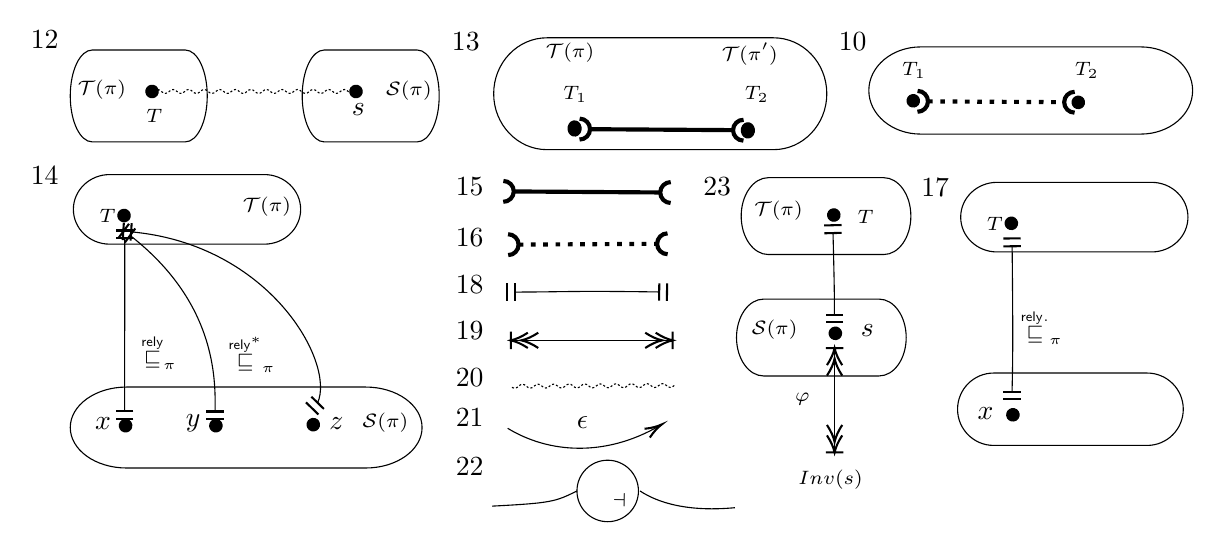
\begin{tikzpicture}[x=0.75pt,y=0.75pt,yscale=-0.75,xscale=0.75]
%uncomment if require: \path (0,1468); %set diagram left start at 0, and has height of 1468

%Straight Lines [id:da9328135073401951] 
\draw [line width=1.5]  [dash pattern={on 1.69pt off 2.76pt}]  (596,452) -- (683.5,452.5) ;
\draw [shift={(683.5,452.5)}, rotate = 0.33] [color={rgb, 255:red, 0; green, 0; blue, 0 }  ][line width=1.5]      (6.71,-6.71) .. controls (3.01,-6.71) and (0,-3.7) .. (0,0) .. controls (0,3.7) and (3.01,6.71) .. (6.71,6.71) ;
\draw [shift={(596,452)}, rotate = 180.33] [color={rgb, 255:red, 0; green, 0; blue, 0 }  ][line width=1.5]      (6.71,-6.71) .. controls (3.01,-6.71) and (0,-3.7) .. (0,0) .. controls (0,3.7) and (3.01,6.71) .. (6.71,6.71) ;
%Shape: Circle [id:dp7632404870091996] 
\draw  [fill={rgb, 255:red, 0; green, 0; blue, 0 }  ,fill opacity=1 ] (696.5,452) .. controls (696.84,454.18) and (695.35,456.23) .. (693.17,456.57) .. controls (690.99,456.92) and (688.94,455.43) .. (688.6,453.25) .. controls (688.25,451.06) and (689.74,449.02) .. (691.93,448.67) .. controls (694.11,448.33) and (696.16,449.82) .. (696.5,452) -- cycle ;
%Shape: Circle [id:dp90868974814637] 
\draw  [fill={rgb, 255:red, 0; green, 0; blue, 0 }  ,fill opacity=1 ] (590.5,451) .. controls (590.84,453.18) and (589.35,455.23) .. (587.17,455.57) .. controls (584.99,455.92) and (582.94,454.43) .. (582.6,452.25) .. controls (582.25,450.06) and (583.74,448.02) .. (585.93,447.67) .. controls (588.11,447.33) and (590.16,448.82) .. (590.5,451) -- cycle ;
%Flowchart: Terminator [id:dp875515007021243] 
\draw   (591.28,417) -- (732.72,417) .. controls (751.1,417) and (766,429.54) .. (766,445) .. controls (766,460.46) and (751.1,473) .. (732.72,473) -- (591.28,473) .. controls (572.9,473) and (558,460.46) .. (558,445) .. controls (558,429.54) and (572.9,417) .. (591.28,417) -- cycle ;
%Shape: Circle [id:dp796186542549407] 
\draw  [fill={rgb, 255:red, 0; green, 0; blue, 0 }  ,fill opacity=1 ] (101.5,445) .. controls (101.84,447.18) and (100.35,449.23) .. (98.17,449.57) .. controls (95.99,449.92) and (93.94,448.43) .. (93.6,446.25) .. controls (93.25,444.06) and (94.74,442.02) .. (96.93,441.67) .. controls (99.11,441.33) and (101.16,442.82) .. (101.5,445) -- cycle ;
%Shape: Circle [id:dp7226784795417869] 
\draw  [fill={rgb, 255:red, 0; green, 0; blue, 0 }  ,fill opacity=1 ] (232.5,445) .. controls (232.84,447.18) and (231.35,449.23) .. (229.17,449.57) .. controls (226.99,449.92) and (224.94,448.43) .. (224.6,446.25) .. controls (224.25,444.06) and (225.74,442.02) .. (227.93,441.67) .. controls (230.11,441.33) and (232.16,442.82) .. (232.5,445) -- cycle ;
%Straight Lines [id:da6908638188904181] 
\draw [line width=1.5]    (378.9,469.85) -- (470.78,470.46) ;
\draw [shift={(470.78,470.46)}, rotate = 0.38] [color={rgb, 255:red, 0; green, 0; blue, 0 }  ][line width=1.5]      (6.71,-6.71) .. controls (3.01,-6.71) and (0,-3.7) .. (0,0) .. controls (0,3.7) and (3.01,6.71) .. (6.71,6.71) ;
\draw [shift={(378.9,469.85)}, rotate = 180.38] [color={rgb, 255:red, 0; green, 0; blue, 0 }  ][line width=1.5]      (6.71,-6.71) .. controls (3.01,-6.71) and (0,-3.7) .. (0,0) .. controls (0,3.7) and (3.01,6.71) .. (6.71,6.71) ;
%Shape: Ellipse [id:dp7488885775277001] 
\draw  [fill={rgb, 255:red, 0; green, 0; blue, 0 }  ,fill opacity=1 ] (484.43,469.85) .. controls (484.79,472.51) and (483.22,475.01) .. (480.93,475.42) .. controls (478.64,475.84) and (476.49,474.03) .. (476.13,471.37) .. controls (475.77,468.71) and (477.33,466.22) .. (479.62,465.8) .. controls (481.91,465.38) and (484.06,467.2) .. (484.43,469.85) -- cycle ;
%Shape: Ellipse [id:dp7887392968433244] 
\draw  [fill={rgb, 255:red, 0; green, 0; blue, 0 }  ,fill opacity=1 ] (373.13,468.64) .. controls (373.49,471.29) and (371.92,473.79) .. (369.63,474.21) .. controls (367.34,474.63) and (365.19,472.81) .. (364.83,470.15) .. controls (364.47,467.5) and (366.03,465) .. (368.32,464.58) .. controls (370.61,464.16) and (372.76,465.98) .. (373.13,468.64) -- cycle ;
%Flowchart: Terminator [id:dp16704563639043535] 
\draw   (351.24,411.14) -- (496.76,411.14) .. controls (515.67,411.14) and (531,427.23) .. (531,447.07) .. controls (531,466.91) and (515.67,483) .. (496.76,483) -- (351.24,483) .. controls (332.33,483) and (317,466.91) .. (317,447.07) .. controls (317,427.23) and (332.33,411.14) .. (351.24,411.14) -- cycle ;
%Flowchart: Terminator [id:dp13936933899200565] 
\draw   (59.08,419) -- (118.92,419) .. controls (126.7,419) and (133,432.21) .. (133,448.5) .. controls (133,464.79) and (126.7,478) .. (118.92,478) -- (59.08,478) .. controls (51.3,478) and (45,464.79) .. (45,448.5) .. controls (45,432.21) and (51.3,419) .. (59.08,419) -- cycle ;
%Flowchart: Terminator [id:dp36692337156365196] 
\draw   (208.08,419) -- (267.92,419) .. controls (275.7,419) and (282,432.21) .. (282,448.5) .. controls (282,464.79) and (275.7,478) .. (267.92,478) -- (208.08,478) .. controls (200.3,478) and (194,464.79) .. (194,448.5) .. controls (194,432.21) and (200.3,419) .. (208.08,419) -- cycle ;
%Straight Lines [id:da7107659391940848] 
\draw  [dash pattern={on 0.75pt off 0.75pt}]  (228.55,445.62) .. controls (226.88,447.29) and (225.22,447.29) .. (223.55,445.62) .. controls (221.88,443.95) and (220.22,443.95) .. (218.55,445.62) .. controls (216.88,447.29) and (215.22,447.29) .. (213.55,445.62) .. controls (211.88,443.95) and (210.22,443.95) .. (208.55,445.62) .. controls (206.88,447.29) and (205.22,447.29) .. (203.55,445.62) .. controls (201.88,443.95) and (200.22,443.95) .. (198.55,445.62) .. controls (196.88,447.29) and (195.22,447.29) .. (193.55,445.62) .. controls (191.88,443.95) and (190.22,443.95) .. (188.55,445.62) .. controls (186.88,447.29) and (185.22,447.29) .. (183.55,445.62) .. controls (181.88,443.95) and (180.22,443.95) .. (178.55,445.62) .. controls (176.88,447.29) and (175.22,447.29) .. (173.55,445.62) .. controls (171.88,443.95) and (170.22,443.95) .. (168.55,445.62) .. controls (166.88,447.29) and (165.22,447.29) .. (163.55,445.62) .. controls (161.88,443.95) and (160.22,443.95) .. (158.55,445.62) .. controls (156.88,447.29) and (155.22,447.29) .. (153.55,445.62) .. controls (151.88,443.95) and (150.22,443.95) .. (148.55,445.62) .. controls (146.88,447.29) and (145.22,447.29) .. (143.55,445.62) .. controls (141.88,443.95) and (140.22,443.95) .. (138.55,445.62) .. controls (136.88,447.29) and (135.22,447.29) .. (133.55,445.62) .. controls (131.88,443.95) and (130.22,443.95) .. (128.55,445.62) .. controls (126.88,447.29) and (125.22,447.29) .. (123.55,445.62) .. controls (121.88,443.95) and (120.22,443.95) .. (118.55,445.62) .. controls (116.88,447.29) and (115.22,447.29) .. (113.55,445.62) .. controls (111.88,443.95) and (110.22,443.95) .. (108.55,445.62) .. controls (106.88,447.29) and (105.22,447.29) .. (103.55,445.62) .. controls (101.88,443.95) and (100.22,443.95) .. (98.55,445.62) -- (97.55,445.62) -- (97.55,445.62) ;
%Curve Lines [id:da9083724795689618] 
\draw [color={rgb, 255:red, 0; green, 0; blue, 0 }  ,draw opacity=1 ]   (79.93,651.07) .. controls (79.94,629.59) and (80,576.57) .. (80,539.98) ;
\draw [shift={(80,539.98)}, rotate = 90] [color={rgb, 255:red, 0; green, 0; blue, 0 }  ,draw opacity=1 ][line width=0.75]    (0,5.59) -- (0,-5.59)(-5.03,5.59) -- (-5.03,-5.59)   ;
\draw [shift={(79.93,651.07)}, rotate = 270] [color={rgb, 255:red, 0; green, 0; blue, 0 }  ,draw opacity=1 ][line width=0.75]    (0,5.59) -- (0,-5.59)(-5.03,5.59) -- (-5.03,-5.59)   ;
%Flowchart: Terminator [id:dp07206252567376059] 
\draw   (70.36,499) -- (169.64,499) .. controls (182.54,499) and (193,509.01) .. (193,521.35) .. controls (193,533.7) and (182.54,543.71) .. (169.64,543.71) -- (70.36,543.71) .. controls (57.46,543.71) and (47,533.7) .. (47,521.35) .. controls (47,509.01) and (57.46,499) .. (70.36,499) -- cycle ;
%Flowchart: Terminator [id:dp391038134175286] 
\draw   (81.16,635.5) -- (234.84,635.5) .. controls (254.81,635.5) and (271,647.14) .. (271,661.5) .. controls (271,675.86) and (254.81,687.5) .. (234.84,687.5) -- (81.16,687.5) .. controls (61.19,687.5) and (45,675.86) .. (45,661.5) .. controls (45,647.14) and (61.19,635.5) .. (81.16,635.5) -- cycle ;
%Shape: Circle [id:dp11812977880680564] 
\draw  [fill={rgb, 255:red, 0; green, 0; blue, 0 }  ,fill opacity=1 ] (84.5,659.71) .. controls (84.84,661.89) and (83.35,663.94) .. (81.17,664.28) .. controls (78.99,664.62) and (76.94,663.13) .. (76.6,660.95) .. controls (76.25,658.77) and (77.74,656.72) .. (79.93,656.38) .. controls (82.11,656.03) and (84.16,657.52) .. (84.5,659.71) -- cycle ;
%Shape: Circle [id:dp8667025155279595] 
\draw  [fill={rgb, 255:red, 0; green, 0; blue, 0 }  ,fill opacity=1 ] (205.07,659.03) .. controls (205.42,661.22) and (203.93,663.26) .. (201.75,663.61) .. controls (199.56,663.95) and (197.52,662.46) .. (197.17,660.28) .. controls (196.83,658.1) and (198.32,656.05) .. (200.5,655.71) .. controls (202.68,655.36) and (204.73,656.85) .. (205.07,659.03) -- cycle ;
%Curve Lines [id:da7282829851271138] 
\draw [color={rgb, 255:red, 0; green, 0; blue, 0 }  ,draw opacity=1 ]   (203.92,645.62) .. controls (215.41,619.66) and (172.96,543.74) .. (84.09,535.81) ;
\draw [shift={(84.09,535.81)}, rotate = 3.69] [color={rgb, 255:red, 0; green, 0; blue, 0 }  ,draw opacity=1 ][line width=0.75]    (0,5.59) -- (0,-5.59)(-5.03,5.59) -- (-5.03,-5.59)   ;
\draw [shift={(203.92,645.62)}, rotate = 314.29] [color={rgb, 255:red, 0; green, 0; blue, 0 }  ,draw opacity=1 ][line width=0.75]    (0,5.59) -- (0,-5.59)(-5.03,5.59) -- (-5.03,-5.59)   ;
%Shape: Circle [id:dp5057910563978223] 
\draw  [fill={rgb, 255:red, 0; green, 0; blue, 0 }  ,fill opacity=1 ] (83.5,524.71) .. controls (83.84,526.89) and (82.35,528.94) .. (80.17,529.28) .. controls (77.99,529.62) and (75.94,528.13) .. (75.6,525.95) .. controls (75.25,523.77) and (76.74,521.72) .. (78.93,521.38) .. controls (81.11,521.03) and (83.16,522.52) .. (83.5,524.71) -- cycle ;
%Shape: Circle [id:dp2925574702853124] 
\draw  [fill={rgb, 255:red, 0; green, 0; blue, 0 }  ,fill opacity=1 ] (142.5,659.71) .. controls (142.84,661.89) and (141.35,663.94) .. (139.17,664.28) .. controls (136.99,664.62) and (134.94,663.13) .. (134.6,660.95) .. controls (134.25,658.77) and (135.74,656.72) .. (137.93,656.38) .. controls (140.11,656.03) and (142.16,657.52) .. (142.5,659.71) -- cycle ;
%Curve Lines [id:da17877027559235592] 
\draw [color={rgb, 255:red, 0; green, 0; blue, 0 }  ,draw opacity=1 ]   (138.01,651.22) .. controls (138.44,630.28) and (138.56,580.99) .. (83.44,538.12) ;
\draw [shift={(83.44,538.12)}, rotate = 36.58] [color={rgb, 255:red, 0; green, 0; blue, 0 }  ,draw opacity=1 ][line width=0.75]    (0,5.59) -- (0,-5.59)(-5.03,5.59) -- (-5.03,-5.59)   ;
\draw [shift={(138.01,651.22)}, rotate = 270] [color={rgb, 255:red, 0; green, 0; blue, 0 }  ,draw opacity=1 ][line width=0.75]    (0,5.59) -- (0,-5.59)(-5.03,5.59) -- (-5.03,-5.59)   ;
%Curve Lines [id:da7822666581011481] 
\draw    (316,712) .. controls (354,710) and (356.5,709.25) .. (370.5,702.25) ;
%Curve Lines [id:da6963621325934628] 
\draw    (411,702.25) .. controls (432,716) and (461,714) .. (472,713) ;
%Shape: Circle [id:dp8782758091128671] 
\draw   (370.5,702.25) .. controls (370.5,691.34) and (379.34,682.5) .. (390.25,682.5) .. controls (401.16,682.5) and (410,691.34) .. (410,702.25) .. controls (410,713.16) and (401.16,722) .. (390.25,722) .. controls (379.34,722) and (370.5,713.16) .. (370.5,702.25) -- cycle ;
%Curve Lines [id:da6439926080689418] 
\draw [color={rgb, 255:red, 0; green, 0; blue, 0 }  ,draw opacity=1 ]   (650.03,638.4) .. controls (650.19,625.91) and (650.86,618.24) .. (650.05,545.06) ;
\draw [shift={(650.05,545.06)}, rotate = 89.34] [color={rgb, 255:red, 0; green, 0; blue, 0 }  ,draw opacity=1 ][line width=0.75]    (0,5.59) -- (0,-5.59)(-5.03,5.59) -- (-5.03,-5.59)   ;
\draw [shift={(650.03,638.4)}, rotate = 270] [color={rgb, 255:red, 0; green, 0; blue, 0 }  ,draw opacity=1 ][line width=0.75]    (0,5.59) -- (0,-5.59)(-5.03,5.59) -- (-5.03,-5.59)   ;
%Flowchart: Terminator [id:dp5946273431848408] 
\draw   (640.36,504) -- (739.64,504) .. controls (752.54,504) and (763,514.01) .. (763,526.35) .. controls (763,538.7) and (752.54,548.71) .. (739.64,548.71) -- (640.36,548.71) .. controls (627.46,548.71) and (617,538.7) .. (617,526.35) .. controls (617,514.01) and (627.46,504) .. (640.36,504) -- cycle ;
%Flowchart: Terminator [id:dp5352037800017746] 
\draw   (638.2,626.5) -- (736.8,626.5) .. controls (749.61,626.5) and (760,636.91) .. (760,649.75) .. controls (760,662.59) and (749.61,673) .. (736.8,673) -- (638.2,673) .. controls (625.39,673) and (615,662.59) .. (615,649.75) .. controls (615,636.91) and (625.39,626.5) .. (638.2,626.5) -- cycle ;
%Shape: Circle [id:dp7028169198049876] 
\draw  [fill={rgb, 255:red, 0; green, 0; blue, 0 }  ,fill opacity=1 ] (654.5,652.71) .. controls (654.84,654.89) and (653.35,656.94) .. (651.17,657.28) .. controls (648.99,657.62) and (646.94,656.13) .. (646.6,653.95) .. controls (646.25,651.77) and (647.74,649.72) .. (649.93,649.38) .. controls (652.11,649.03) and (654.16,650.52) .. (654.5,652.71) -- cycle ;
%Shape: Circle [id:dp9682999612019707] 
\draw  [fill={rgb, 255:red, 0; green, 0; blue, 0 }  ,fill opacity=1 ] (653.5,529.71) .. controls (653.84,531.89) and (652.35,533.94) .. (650.17,534.28) .. controls (647.99,534.62) and (645.94,533.13) .. (645.6,530.95) .. controls (645.25,528.77) and (646.74,526.72) .. (648.93,526.38) .. controls (651.11,526.03) and (653.16,527.52) .. (653.5,529.71) -- cycle ;
%Straight Lines [id:da21744917459599944] 
\draw [line width=1.5]    (329.9,509.85) -- (424,510.5) ;
\draw [shift={(424,510.5)}, rotate = 0.39] [color={rgb, 255:red, 0; green, 0; blue, 0 }  ][line width=1.5]      (6.71,-6.71) .. controls (3.01,-6.71) and (0,-3.7) .. (0,0) .. controls (0,3.7) and (3.01,6.71) .. (6.71,6.71) ;
\draw [shift={(329.9,509.85)}, rotate = 180.39] [color={rgb, 255:red, 0; green, 0; blue, 0 }  ][line width=1.5]      (6.71,-6.71) .. controls (3.01,-6.71) and (0,-3.7) .. (0,0) .. controls (0,3.7) and (3.01,6.71) .. (6.71,6.71) ;
%Straight Lines [id:da16257929947618766] 
\draw [line width=1.5]  [dash pattern={on 1.69pt off 2.76pt}]  (333,544) -- (422,543.5) ;
\draw [shift={(422,543.5)}, rotate = 359.68] [color={rgb, 255:red, 0; green, 0; blue, 0 }  ][line width=1.5]      (6.71,-6.71) .. controls (3.01,-6.71) and (0,-3.7) .. (0,0) .. controls (0,3.7) and (3.01,6.71) .. (6.71,6.71) ;
\draw [shift={(333,544)}, rotate = 179.68] [color={rgb, 255:red, 0; green, 0; blue, 0 }  ][line width=1.5]      (6.71,-6.71) .. controls (3.01,-6.71) and (0,-3.7) .. (0,0) .. controls (0,3.7) and (3.01,6.71) .. (6.71,6.71) ;
%Curve Lines [id:da8676022514493338] 
\draw [color={rgb, 255:red, 0; green, 0; blue, 0 }  ,draw opacity=1 ]   (423.32,574.42) .. controls (366.64,573.6) and (363.08,574.42) .. (330.77,574.49) ;
\draw [shift={(330.77,574.49)}, rotate = 360] [color={rgb, 255:red, 0; green, 0; blue, 0 }  ,draw opacity=1 ][line width=0.75]    (0,5.59) -- (0,-5.59)(-5.03,5.59) -- (-5.03,-5.59)   ;
\draw [shift={(423.32,574.42)}, rotate = 180.88] [color={rgb, 255:red, 0; green, 0; blue, 0 }  ,draw opacity=1 ][line width=0.75]    (0,5.59) -- (0,-5.59)(-5.03,5.59) -- (-5.03,-5.59)   ;
%Straight Lines [id:da5957423543666296] 
\draw    (328,605.5) -- (432,605.5) ;
\draw [shift={(432,605.5)}, rotate = 180] [color={rgb, 255:red, 0; green, 0; blue, 0 }  ][line width=0.75]    (0,5.59) -- (0,-5.59)(17.64,-4.9) .. controls (13.66,-2.3) and (10.02,-0.67) .. (6.71,0) .. controls (10.02,0.67) and (13.66,2.3) .. (17.64,4.9)(10.93,-4.9) .. controls (6.95,-2.3) and (3.31,-0.67) .. (0,0) .. controls (3.31,0.67) and (6.95,2.3) .. (10.93,4.9)   ;
\draw [shift={(328,605.5)}, rotate = 0] [color={rgb, 255:red, 0; green, 0; blue, 0 }  ][line width=0.75]    (0,5.59) -- (0,-5.59)(17.64,-4.9) .. controls (13.66,-2.3) and (10.02,-0.67) .. (6.71,0) .. controls (10.02,0.67) and (13.66,2.3) .. (17.64,4.9)(10.93,-4.9) .. controls (6.95,-2.3) and (3.31,-0.67) .. (0,0) .. controls (3.31,0.67) and (6.95,2.3) .. (10.93,4.9)   ;
%Curve Lines [id:da08316429581034357] 
\draw    (326,662) .. controls (352.6,678.25) and (388.89,680.44) .. (423.42,660.43) ;
\draw [shift={(425,659.5)}, rotate = 149.04] [color={rgb, 255:red, 0; green, 0; blue, 0 }  ][line width=0.75]    (10.93,-3.29) .. controls (6.95,-1.4) and (3.31,-0.3) .. (0,0) .. controls (3.31,0.3) and (6.95,1.4) .. (10.93,3.29)   ;
%Straight Lines [id:da5364075364264385] 
\draw  [dash pattern={on 0.75pt off 0.75pt}]  (433,634.5) .. controls (431.34,636.17) and (429.67,636.18) .. (428,634.52) .. controls (426.33,632.87) and (424.66,632.88) .. (423,634.55) .. controls (421.34,636.22) and (419.67,636.23) .. (418,634.57) .. controls (416.33,632.92) and (414.66,632.93) .. (413,634.6) .. controls (411.34,636.27) and (409.67,636.28) .. (408,634.62) .. controls (406.33,632.96) and (404.66,632.97) .. (403,634.64) .. controls (401.34,636.31) and (399.67,636.32) .. (398,634.67) .. controls (396.33,633.01) and (394.66,633.02) .. (393,634.69) .. controls (391.34,636.36) and (389.67,636.37) .. (388,634.71) .. controls (386.33,633.06) and (384.66,633.07) .. (383,634.74) .. controls (381.34,636.41) and (379.67,636.42) .. (378,634.76) .. controls (376.33,633.11) and (374.66,633.12) .. (373,634.79) .. controls (371.34,636.46) and (369.67,636.47) .. (368,634.81) .. controls (366.33,633.15) and (364.66,633.16) .. (363,634.83) .. controls (361.34,636.5) and (359.67,636.51) .. (358,634.86) .. controls (356.33,633.2) and (354.66,633.21) .. (353,634.88) .. controls (351.34,636.55) and (349.67,636.56) .. (348,634.9) .. controls (346.33,633.25) and (344.66,633.26) .. (343,634.93) .. controls (341.34,636.6) and (339.67,636.61) .. (338,634.95) .. controls (336.33,633.3) and (334.66,633.31) .. (333,634.98) .. controls (331.34,636.65) and (329.67,636.66) .. (328,635) -- (328,635) -- (328,635) ;
%Shape: Circle [id:dp5741933897518225] 
\draw  [fill={rgb, 255:red, 0; green, 0; blue, 0 }  ,fill opacity=1 ] (540.45,600.38) .. controls (540.8,602.56) and (539.31,604.61) .. (537.12,604.95) .. controls (534.94,605.3) and (532.89,603.81) .. (532.55,601.62) .. controls (532.2,599.44) and (533.69,597.39) .. (535.88,597.05) .. controls (538.06,596.7) and (540.11,598.19) .. (540.45,600.38) -- cycle ;
%Straight Lines [id:da11633558579225434] 
\draw    (536,610.5) -- (536,677.5) ;
\draw [shift={(536,677.5)}, rotate = 270] [color={rgb, 255:red, 0; green, 0; blue, 0 }  ][line width=0.75]    (0,5.59) -- (0,-5.59)(17.64,-4.9) .. controls (13.66,-2.3) and (10.02,-0.67) .. (6.71,0) .. controls (10.02,0.67) and (13.66,2.3) .. (17.64,4.9)(10.93,-4.9) .. controls (6.95,-2.3) and (3.31,-0.67) .. (0,0) .. controls (3.31,0.67) and (6.95,2.3) .. (10.93,4.9)   ;
\draw [shift={(536,610.5)}, rotate = 90] [color={rgb, 255:red, 0; green, 0; blue, 0 }  ][line width=0.75]    (0,5.59) -- (0,-5.59)(17.64,-4.9) .. controls (13.66,-2.3) and (10.02,-0.67) .. (6.71,0) .. controls (10.02,0.67) and (13.66,2.3) .. (17.64,4.9)(10.93,-4.9) .. controls (6.95,-2.3) and (3.31,-0.67) .. (0,0) .. controls (3.31,0.67) and (6.95,2.3) .. (10.93,4.9)   ;
%Flowchart: Terminator [id:dp18564493986257768] 
\draw   (490.44,579) -- (564.56,579) .. controls (574.19,579) and (582,590.05) .. (582,603.69) .. controls (582,617.32) and (574.19,628.38) .. (564.56,628.38) -- (490.44,628.38) .. controls (480.81,628.38) and (473,617.32) .. (473,603.69) .. controls (473,590.05) and (480.81,579) .. (490.44,579) -- cycle ;
%Flowchart: Terminator [id:dp5885594659003628] 
\draw   (493.44,501) -- (567.56,501) .. controls (577.19,501) and (585,512.05) .. (585,525.69) .. controls (585,539.32) and (577.19,550.38) .. (567.56,550.38) -- (493.44,550.38) .. controls (483.81,550.38) and (476,539.32) .. (476,525.69) .. controls (476,512.05) and (483.81,501) .. (493.44,501) -- cycle ;
%Shape: Circle [id:dp4446972352348635] 
\draw  [fill={rgb, 255:red, 0; green, 0; blue, 0 }  ,fill opacity=1 ] (539.45,524.38) .. controls (539.8,526.56) and (538.31,528.61) .. (536.12,528.95) .. controls (533.94,529.3) and (531.89,527.81) .. (531.55,525.62) .. controls (531.2,523.44) and (532.69,521.39) .. (534.88,521.05) .. controls (537.06,520.7) and (539.11,522.19) .. (539.45,524.38) -- cycle ;
%Curve Lines [id:da1173213301666387] 
\draw [color={rgb, 255:red, 0; green, 0; blue, 0 }  ,draw opacity=1 ]   (535.88,588.94) .. controls (535.89,576.8) and (535.88,571.59) .. (534.99,536.58) ;
\draw [shift={(534.99,536.58)}, rotate = 88.54] [color={rgb, 255:red, 0; green, 0; blue, 0 }  ,draw opacity=1 ][line width=0.75]    (0,5.59) -- (0,-5.59)(-5.03,5.59) -- (-5.03,-5.59)   ;
\draw [shift={(535.88,588.94)}, rotate = 270] [color={rgb, 255:red, 0; green, 0; blue, 0 }  ,draw opacity=1 ][line width=0.75]    (0,5.59) -- (0,-5.59)(-5.03,5.59) -- (-5.03,-5.59)   ;

% Text Node
\draw (587,432) node  [font=\scriptsize]  {$T_{1}{}$};
% Text Node
\draw (698,432) node  [font=\scriptsize]  {$T_{2}{}$};
% Text Node
\draw (537,406) node [anchor=north west][inner sep=0.75pt]  [color={rgb, 255:red, 0; green, 0; blue, 0 }  ,opacity=1 ] [align=left] {10};
% Text Node
\draw (99,461) node  [font=\scriptsize]  {$T$};
% Text Node
\draw (230,457) node    {$s$};
% Text Node
\draw (18,405) node [anchor=north west][inner sep=0.75pt]  [color={rgb, 255:red, 0; green, 0; blue, 0 }  ,opacity=1 ] [align=left] {12};
% Text Node
\draw (348.73,412.7) node [anchor=north west][inner sep=0.75pt]  [font=\scriptsize] [align=left] {$\displaystyle \mathcal{T}( \pi )$};
% Text Node
\draw (369.45,447.5) node  [font=\scriptsize]  {$T_{1}{}$};
% Text Node
\draw (486,447.5) node  [font=\scriptsize]  {$T_{2}{}$};
% Text Node
\draw (288.5,406.4) node [anchor=north west][inner sep=0.75pt]  [color={rgb, 255:red, 0; green, 0; blue, 0 }  ,opacity=1 ] [align=left] {13};
% Text Node
\draw (48,436.29) node [anchor=north west][inner sep=0.75pt]  [font=\scriptsize] [align=left] {$\displaystyle \mathcal{T}( \pi )$};
% Text Node
\draw (246,437) node [anchor=north west][inner sep=0.75pt]  [font=\scriptsize] [align=left] {$\displaystyle \mathcal{S}( \pi )$};
% Text Node
\draw (461.73,412.7) node [anchor=north west][inner sep=0.75pt]  [font=\scriptsize] [align=left] {$\displaystyle \mathcal{T}( \pi ')$};
% Text Node
\draw  [color={rgb, 255:red, 255; green, 255; blue, 255 }  ,draw opacity=1 ][fill={rgb, 255:red, 255; green, 255; blue, 255 }  ,fill opacity=1 ]  (96.5, 610) circle [x radius= 9.19, y radius= 12.73]   ;
\draw (89,600) node [anchor=north west][inner sep=0.75pt]  [font=\scriptsize] [align=left] {$\overset{\mathsf{rely}}{\sqsubseteq}_{\pi}$};
% Text Node
\draw (154,511.71) node [anchor=north west][inner sep=0.75pt]  [font=\scriptsize] [align=left] {$\displaystyle \mathcal{T}( \pi )$};
% Text Node
\draw (69,525.71) node  [font=\scriptsize]  {$T$};
% Text Node
\draw (231,650.71) node [anchor=north west][inner sep=0.75pt]  [font=\scriptsize] [align=left] {$\displaystyle \mathcal{S}( \pi )$};
% Text Node
\draw (66,658.71) node    {$x$};
% Text Node
\draw (216,658.71) node    {$z$};
% Text Node
\draw (124,658.71) node    {$y$};
% Text Node
\draw  [color={rgb, 255:red, 255; green, 255; blue, 255 }  ,draw opacity=1 ][fill={rgb, 255:red, 255; green, 255; blue, 255 }  ,fill opacity=1 ]  (152.5, 610) circle [x radius= 9.19, y radius= 12.73]   ;
\draw (145,600) node [anchor=north west][inner sep=0.75pt]  [font=\scriptsize] [align=left] {$\overset{\mathsf{rely}^{*}}{\sqsubseteq}_{\pi}$};
% Text Node
\draw (18,492) node [anchor=north west][inner sep=0.75pt]  [color={rgb, 255:red, 0; green, 0; blue, 0 }  ,opacity=1 ] [align=left] {14};
% Text Node
\draw (403.82,714.22) node [anchor=north west][inner sep=0.75pt]  [font=\scriptsize,rotate=-180.87] [align=left] {$\displaystyle \vdash $};
% Text Node
\draw (291,679) node [anchor=north west][inner sep=0.75pt]  [color={rgb, 255:red, 0; green, 0; blue, 0 }  ,opacity=1 ] [align=left] {22};
% Text Node
\draw  [color={rgb, 255:red, 255; green, 255; blue, 255 }  ,draw opacity=1 ][fill={rgb, 255:red, 255; green, 255; blue, 255 }  ,fill opacity=1 ]  (661.5, 594) circle [x radius= 9.19, y radius= 12.73]   ;
\draw (654,584) node [anchor=north west][inner sep=0.75pt]  [font=\scriptsize] [align=left] {$\overset{\mathsf{rely.}}{\sqsubseteq}_{\pi}$};
% Text Node
\draw (639,530.71) node  [font=\scriptsize]  {$T$};
% Text Node
\draw (633,652.71) node    {$x$};
% Text Node
\draw (590,500) node [anchor=north west][inner sep=0.75pt]  [color={rgb, 255:red, 0; green, 0; blue, 0 }  ,opacity=1 ] [align=left] {17};
% Text Node
\draw (374,658) node    {$\epsilon$};
% Text Node
\draw (291,499) node [anchor=north west][inner sep=0.75pt]  [color={rgb, 255:red, 0; green, 0; blue, 0 }  ,opacity=1 ] [align=left] {15};
% Text Node
\draw (291,532) node [anchor=north west][inner sep=0.75pt]  [color={rgb, 255:red, 0; green, 0; blue, 0 }  ,opacity=1 ] [align=left] {16};
% Text Node
\draw (291,562) node [anchor=north west][inner sep=0.75pt]  [color={rgb, 255:red, 0; green, 0; blue, 0 }  ,opacity=1 ] [align=left] {18};
% Text Node
\draw (291,592) node [anchor=north west][inner sep=0.75pt]  [color={rgb, 255:red, 0; green, 0; blue, 0 }  ,opacity=1 ] [align=left] {19};
% Text Node
\draw (291,622) node [anchor=north west][inner sep=0.75pt]  [color={rgb, 255:red, 0; green, 0; blue, 0 }  ,opacity=1 ] [align=left] {20};
% Text Node
\draw (291,648) node [anchor=north west][inner sep=0.75pt]  [color={rgb, 255:red, 0; green, 0; blue, 0 }  ,opacity=1 ] [align=left] {21};
% Text Node
\draw (481,591) node [anchor=north west][inner sep=0.75pt]  [font=\scriptsize] [align=left] {$\displaystyle \mathcal{S}( \pi )$};
% Text Node
\draw (557,599) node    {$s$};
% Text Node
\draw (511,687) node [anchor=north west][inner sep=0.75pt]  [font=\scriptsize] [align=left] {$\displaystyle Inv( s )$};
% Text Node
\draw (509,638) node [anchor=north west][inner sep=0.75pt]  [font=\scriptsize] [align=left] {$\displaystyle \varphi $};
% Text Node
\draw (450,499) node [anchor=north west][inner sep=0.75pt]  [color={rgb, 255:red, 0; green, 0; blue, 0 }  ,opacity=1 ] [align=left] {23};
% Text Node
\draw (482.62,514) node [anchor=north west][inner sep=0.75pt]  [font=\scriptsize] [align=left] {$\displaystyle \mathcal{T}( \pi )$};
% Text Node
\draw (556,526) node  [font=\scriptsize]  {$T$};
\end{tikzpicture}
\end{figure}
\end{frame}

\begin{frame}{We Need This} \scriptsize
\[
\inferrule[Bisim]{
	\pi\sim\pi'\quad\quad 
	q\; \epsilon_{\mathcal{S}} \;s \quad\quad q' \; \epsilon_{\mathcal{S}} \;s' \\
	\triple{\ownGhost{\gamma}{s;\epsilon_{\overline{\mathcal{T}}}(\mathcal{T})}_{\pi'} \ast P}{C}{\ownGhost{\gamma}{s';\mathsf{T}'}_{\pi'} \ast Q}
}{
	\fbox{$\varphi$}^{\gamma}_{\pi} \vdash
    \triple{\ownGhost{\gamma}{q;\mathsf{T}}_{\pi}\ast P}{C}{\ownGhost{\gamma}{q';\mathsf{T}'}_{\pi} \ast Q}
}
\]
\end{frame}
\begin{frame}{We Use This}\scriptsize
\[
\inferrule[UpdIsl]{
        \alpha~\textrm{physically atomic}\\
        \forall s_0 \;\ldotp  \;((s;\mathsf{T})\;\overset{\mathsf{rely}^{*}}{\sqsubseteq}_\pi\;( s_0;\mathsf{T}))\; \vdash
        \triple{ \varphi(s_0)\ast P }{\alpha}{ \exists s' \;, \;\mathsf{T}'\;\ldotp \; (s_0;\mathsf{T})\; \overset{\mathsf{guar}^{*}}{\sqsubseteq}_\pi \;(s';\mathsf{T}') \ast 
        \varphi(s')\ast Q}
    }{
      \fbox{$\varphi$}^{\gamma}_{\pi} \vdash
      \triple{ \ownGhost{\gamma}{s;\mathsf{T}} \ast P }
            {\alpha}
        { \exists \; s', \mathsf{T}' \ldotp \ownGhost{\gamma}{s';\mathsf{T}'} \ast Q }
    }
\]
\[
\inferrule[Bisim]{
	\pi\sim\pi'\quad\quad 
	q\; \epsilon_{\mathcal{S}} \;s \quad\quad q' \; \epsilon_{\mathcal{S}} \;s' \\
	\triple{\ownGhost{\gamma}{s;\epsilon_{\overline{\mathcal{T}}}(\mathcal{T})}_{\pi'} \ast P}{C}{\ownGhost{\gamma}{s';\mathsf{T}'}_{\pi'} \ast Q}
}{
	\fbox{$\varphi$}^{\gamma}_{\pi} \vdash
    \triple{\ownGhost{\gamma}{q;\mathsf{T}}_{\pi}\ast P}{C}{\ownGhost{\gamma}{q';\mathsf{T}'}_{\pi} \ast Q}
}
\]
\end{frame}
\begin{frame}{How? Obligation - 1}\scriptsize
\[
\inferrule[UpdIsl]{
        \alpha~\textrm{physically atomic}\\
        \forall s_0 \;\ldotp  \;\tcbhighmath[boxrule=2pt,arc=1pt,colback=blue!10!white,colframe=blue,
  drop fuzzy shadow=red]{((s;\mathsf{T})\;\overset{\mathsf{rely}^{*}}{\sqsubseteq}_\pi\;( s_0;\mathsf{T}))}\; \vdash
        \triple{ \varphi(s_0)\ast P }{\alpha}{ \exists s' \;, \;\mathsf{T}'\;\ldotp \; (s_0;\mathsf{T})\; \overset{\mathsf{guar}^{*}}{\sqsubseteq}_\pi \;(s';\mathsf{T}') \ast 
        \varphi(s')\ast Q}
    }{
      \fbox{$\varphi$}^{\gamma}_{\pi} \vdash
      \triple{ \ownGhost{\gamma}{s;\mathsf{T}}_{\pi} \ast P }
            {\alpha}
        { \exists \; s', \mathsf{T}' \ldotp \ownGhost{\gamma}{s';\mathsf{T}'}_{\pi} \ast Q }
    }
\]
\[
\inferrule[Bisim]{
	\pi\sim\pi'\quad\quad 
	q\; \epsilon_{\mathcal{S}} \;s \quad\quad q' \; \epsilon_{\mathcal{S}} \;s' \\
	\triple{\ownGhost{\gamma}{s;\epsilon_{\overline{\mathcal{T}}}(\mathcal{T})}_{\pi'} \ast P}{C}{\ownGhost{\gamma}{s';\mathsf{T}'}_{\pi'} \ast Q}
}{
	\fbox{$\varphi$}^{\gamma}_{\pi} \vdash
    \triple{\ownGhost{\gamma}{q;\mathsf{T}}_{\pi}\ast P}{C}{\ownGhost{\gamma}{q';\mathsf{T}'}_{\pi} \ast Q}
}
\]
\end{frame}
\begin{frame}{The Law of Rely}\scriptsize
 \begin{theorem}[The Law of Rely]\scriptsize
            \[
            \begin{array}{l}\forall s' .   (s;T) \overset{\mathsf{rely}^{*}}{\sqsubseteq}_{\pi}  (s';T) \leftrightarrow \\
           \quad\quad  (\forall_{s_1,s_1',T_1} \ldotp \epsilon_{\mathcal{S}}(s ,s_1) \rightarrow \epsilon_{\mathcal{S}}(s',s'_1) \rightarrow \epsilon_{\overline{\mathcal{T}}}(T,T_1) \rightarrow ( s_1; T_1) \overset{\mathsf{rely}^{*}}{\sqsubseteq}_{\pi'} (s'_1; T_1)
            \end{array}
           \]
     \end{theorem}
     \begin{itemize}
         \item We do not drop any client interference with capabilities $T$
         \item Indetification of the states that are tolerant to the client interference from which the STS can take steps (Guarantee)
         \item Bookkeeping of the client interference needed!  
         \item Identifying the valid \emph{pre} state
     \end{itemize}
\end{frame}
\begin{frame}{The Law of Rely}\scriptsize
\begin{figure}
\scriptsize
    \centering
\tikzset {_ofpsgqcy8/.code = {\pgfsetadditionalshadetransform{ \pgftransformshift{\pgfpoint{0 bp } { 0 bp }  }  \pgftransformrotate{0 }  \pgftransformscale{2 }  }}}
\pgfdeclarehorizontalshading{_myriwypn8}{150bp}{rgb(0bp)=(0.27,0.28,0.3);
rgb(37.5bp)=(0.27,0.28,0.3);
rgb(62.5bp)=(0,0,0);
rgb(100bp)=(0,0,0)}
\tikzset{every picture/.style={line width=0.75pt}} %set default line width to 0.75pt        

\begin{tikzpicture}[x=0.75pt,y=0.75pt,yscale=-0.7,xscale=0.7]
%uncomment if require: \path (0,368); %set diagram left start at 0, and has height of 368

%Shape: Circle [id:dp31461291036449346] 
\draw  [fill={rgb, 255:red, 0; green, 0; blue, 0 }  ,fill opacity=1 ] (68.95,258.38) .. controls (69.3,260.56) and (67.81,262.61) .. (65.62,262.95) .. controls (63.44,263.3) and (61.39,261.81) .. (61.05,259.62) .. controls (60.7,257.44) and (62.19,255.39) .. (64.38,255.05) .. controls (66.56,254.7) and (68.61,256.19) .. (68.95,258.38) -- cycle ;
%Shape: Circle [id:dp33974947625378027] 
\draw  [fill={rgb, 255:red, 0; green, 0; blue, 0 }  ,fill opacity=1 ] (108.95,83.38) .. controls (109.3,85.56) and (107.81,87.61) .. (105.62,87.95) .. controls (103.44,88.3) and (101.39,86.81) .. (101.05,84.62) .. controls (100.7,82.44) and (102.19,80.39) .. (104.38,80.05) .. controls (106.56,79.7) and (108.61,81.19) .. (108.95,83.38) -- cycle ;
%Curve Lines [id:da9654456846856758] 
\draw [color={rgb, 255:red, 0; green, 0; blue, 0 }  ,draw opacity=1 ]   (71.64,245.72) .. controls (95.83,214.69) and (100.93,152.38) .. (104.71,93.52) ;
\draw [shift={(104.71,93.52)}, rotate = 93.63] [color={rgb, 255:red, 0; green, 0; blue, 0 }  ,draw opacity=1 ][line width=0.75]    (0,5.59) -- (0,-5.59)(-5.03,5.59) -- (-5.03,-5.59)   ;
\draw [shift={(71.64,245.72)}, rotate = 313.03] [color={rgb, 255:red, 0; green, 0; blue, 0 }  ,draw opacity=1 ][line width=0.75]    (0,5.59) -- (0,-5.59)(-5.03,5.59) -- (-5.03,-5.59)   ;
%Curve Lines [id:da5554639324183348] 
\draw [color={rgb, 255:red, 0; green, 0; blue, 0 }  ,draw opacity=1 ]   (191.1,247.77) .. controls (232.5,213.78) and (203.12,112.5) .. (116.02,90.93) ;
\draw [shift={(116.02,90.93)}, rotate = 12.14] [color={rgb, 255:red, 0; green, 0; blue, 0 }  ,draw opacity=1 ][line width=0.75]    (0,5.59) -- (0,-5.59)(-5.03,5.59) -- (-5.03,-5.59)   ;
\draw [shift={(191.1,247.77)}, rotate = 327.14] [color={rgb, 255:red, 0; green, 0; blue, 0 }  ,draw opacity=1 ][line width=0.75]    (0,5.59) -- (0,-5.59)(-5.03,5.59) -- (-5.03,-5.59)   ;
%Flowchart: Terminator [id:dp3449465191729819] 
\draw   (92,5) -- (364,5) .. controls (399.35,5) and (428,32.31) .. (428,66) .. controls (428,99.69) and (399.35,127) .. (364,127) -- (92,127) .. controls (56.65,127) and (28,99.69) .. (28,66) .. controls (28,32.31) and (56.65,5) .. (92,5) -- cycle ;
%Flowchart: Terminator [id:dp4741510968252982] 
\draw   (91.33,223) -- (363.87,223) .. controls (399.29,223) and (428,250.31) .. (428,284) .. controls (428,317.69) and (399.29,345) .. (363.87,345) -- (91.33,345) .. controls (55.91,345) and (27.2,317.69) .. (27.2,284) .. controls (27.2,250.31) and (55.91,223) .. (91.33,223) -- cycle ;
%Curve Lines [id:da06836526078807603] 
\draw    (191,270) .. controls (198.92,304.65) and (301.91,303.04) .. (343.14,283.72) ;
\draw [shift={(344.38,283.13)}, rotate = 153.79] [color={rgb, 255:red, 0; green, 0; blue, 0 }  ][line width=0.75]    (10.93,-3.29) .. controls (6.95,-1.4) and (3.31,-0.3) .. (0,0) .. controls (3.31,0.3) and (6.95,1.4) .. (10.93,3.29)   ;
%Curve Lines [id:da5104481747535965] 
\draw    (69,268) .. controls (86.73,295.58) and (215.07,298.9) .. (250.45,278.93) ;
\draw [shift={(252,278)}, rotate = 147.53] [color={rgb, 255:red, 0; green, 0; blue, 0 }  ][line width=0.75]    (10.93,-3.29) .. controls (6.95,-1.4) and (3.31,-0.3) .. (0,0) .. controls (3.31,0.3) and (6.95,1.4) .. (10.93,3.29)   ;
%Curve Lines [id:da12451452612867331] 
\draw [color={rgb, 255:red, 0; green, 0; blue, 0 }  ,draw opacity=1 ]   (371.15,262.25) .. controls (446.11,230.22) and (428.82,105.64) .. (347.15,93.6) ;
\draw [shift={(347.15,93.6)}, rotate = 5.85] [color={rgb, 255:red, 0; green, 0; blue, 0 }  ,draw opacity=1 ][line width=0.75]    (0,5.59) -- (0,-5.59)(-5.03,5.59) -- (-5.03,-5.59)   ;
\draw [shift={(371.15,262.25)}, rotate = 340.36] [color={rgb, 255:red, 0; green, 0; blue, 0 }  ,draw opacity=1 ][line width=0.75]    (0,5.59) -- (0,-5.59)(-5.03,5.59) -- (-5.03,-5.59)   ;
%Curve Lines [id:da9919788095840558] 
\draw [color={rgb, 255:red, 0; green, 0; blue, 0 }  ,draw opacity=1 ]   (275.33,242.41) .. controls (305.58,200.83) and (350.93,142.01) .. (334.69,97.12) ;
\draw [shift={(334.69,97.12)}, rotate = 65.42] [color={rgb, 255:red, 0; green, 0; blue, 0 }  ,draw opacity=1 ][line width=0.75]    (0,5.59) -- (0,-5.59)(-5.03,5.59) -- (-5.03,-5.59)   ;
\draw [shift={(275.33,242.41)}, rotate = 305.79] [color={rgb, 255:red, 0; green, 0; blue, 0 }  ,draw opacity=1 ][line width=0.75]    (0,5.59) -- (0,-5.59)(-5.03,5.59) -- (-5.03,-5.59)   ;
%Straight Lines [id:da35317307415111254] 
\draw    (119.5,80) -- (323.01,60.19) ;
\draw [shift={(325,60)}, rotate = 174.44] [color={rgb, 255:red, 0; green, 0; blue, 0 }  ][line width=0.75]    (10.93,-3.29) .. controls (6.95,-1.4) and (3.31,-0.3) .. (0,0) .. controls (3.31,0.3) and (6.95,1.4) .. (10.93,3.29)   ;
%Shape: Regular Polygon [id:dp22598651457897012] 
\path  [shading=_myriwypn8,_ofpsgqcy8] (192.55,264.2) -- (186.99,277.63) -- (173.55,283.2) -- (160.12,277.63) -- (154.55,264.2) -- (160.12,250.76) -- (173.55,245.2) -- (186.99,250.76) -- cycle ; % for fading 
 \draw   (192.55,264.2) -- (186.99,277.63) -- (173.55,283.2) -- (160.12,277.63) -- (154.55,264.2) -- (160.12,250.76) -- (173.55,245.2) -- (186.99,250.76) -- cycle ; % for border 

%Shape: Regular Polygon [id:dp6390986486773769] 
\draw  [fill={rgb, 255:red, 255; green, 255; blue, 255 }  ,fill opacity=1 ] (362.13,74.38) -- (356.63,87.63) -- (343.38,93.13) -- (330.12,87.63) -- (324.63,74.38) -- (330.12,61.12) -- (343.38,55.63) -- (356.63,61.12) -- cycle ;
%Shape: Regular Polygon [id:dp6042023471043982] 
\draw  [fill={rgb, 255:red, 255; green, 255; blue, 255 }  ,fill opacity=1 ] (363.13,264.38) -- (357.63,277.63) -- (344.38,283.13) -- (331.12,277.63) -- (325.63,264.38) -- (331.12,251.12) -- (344.38,245.63) -- (357.63,251.12) -- cycle ;
%Shape: Regular Polygon [id:dp2660336147384734] 
\draw  [fill={rgb, 255:red, 255; green, 255; blue, 255 }  ,fill opacity=1 ] (290.13,264.38) -- (284.63,277.63) -- (271.38,283.13) -- (258.12,277.63) -- (252.63,264.38) -- (258.12,251.12) -- (271.38,245.63) -- (284.63,251.12) -- cycle ;

% Text Node
\draw (87,16) node [anchor=north west][inner sep=0.75pt]  [font=\scriptsize] [align=left] {$\displaystyle \mathcal{T}( \pi )$};
% Text Node
\draw (328,16) node [anchor=north west][inner sep=0.75pt]  [font=\scriptsize] [align=left] {$\displaystyle \mathcal{T}( \pi ')$};
% Text Node
\draw (253,321) node [anchor=north west][inner sep=0.75pt]  [font=\scriptsize] [align=left] {$\displaystyle \mathcal{S}( \pi ')$};
% Text Node
\draw (159,321) node [anchor=north west][inner sep=0.75pt]  [font=\scriptsize] [align=left] {$\displaystyle \mathcal{S}( \pi )$};
% Text Node
\draw (87,86) node  [font=\scriptsize]  {$T$};
% Text Node
\draw (377,67) node  [font=\scriptsize]  {$T_{1}$};
% Text Node
\draw (150,242) node    {$s'$};
% Text Node
\draw (50,260) node    {$s$};
% Text Node
\draw  [color={rgb, 255:red, 255; green, 255; blue, 255 }  ,draw opacity=1 ][fill={rgb, 255:red, 255; green, 255; blue, 255 }  ,fill opacity=1 ]  (124, 180) circle [x radius= 9.9, y radius= 12.73]   ;
\draw (118,173) node [anchor=north west][inner sep=0.75pt]  [font=\scriptsize] [align=left] {$\overset{\mathsf{rely}^{*}}{\sqsubseteq}_{\pi}$};
% Text Node
\draw  [color={rgb, 255:red, 255; green, 255; blue, 255 }  ,draw opacity=1 ][fill={rgb, 255:red, 255; green, 255; blue, 255 }  ,fill opacity=1 ]  (346.5, 180) circle [x radius= 9.19, y radius= 12.73]   ;
\draw (341,173) node [anchor=north west][inner sep=0.75pt]  [font=\scriptsize] [align=left] {$\overset{\mathsf{rely}^{*}}{\sqsubseteq}_{\pi'}$};
% Text Node
\draw (373,242) node    {$s'_{1}$};
% Text Node
\draw (300,242) node    {$s_{1}$};
% Text Node
\draw (116,302) node    {$\epsilon_{\mathcal{S}}$};
% Text Node
\draw (316,306) node    {$\epsilon_{\mathcal{S}}$};
% Text Node
\draw (205,51) node  [font=\scriptsize]  {$\epsilon_{\overline{\mathcal{T}}}$};
% Text Node
\draw (338.12,66.12) node [anchor=north west][inner sep=0.75pt]  [color={rgb, 255:red, 0; green, 0; blue, 0 }  ,opacity=1 ] [align=left] {n};
% Text Node
\draw (339.12,256.12) node [anchor=north west][inner sep=0.75pt]  [color={rgb, 255:red, 0; green, 0; blue, 0 }  ,opacity=1 ] [align=left] {n};
% Text Node
\draw (266.12,256.12) node [anchor=north west][inner sep=0.75pt]  [color={rgb, 255:red, 0; green, 0; blue, 0 }  ,opacity=1 ] [align=left] {n};


\end{tikzpicture}
    \caption{Embedding The Client Interface}
    \label{fig:enter-label}
\end{figure}
    
\end{frame}
\begin{frame}{The Law of Rely for a Bisimulation Instance} \scriptsize
    \begin{columns}
        \column{0.5\textwidth}
        \begin{figure}\scriptsize



% Gradient Info
  
\tikzset {_c4bheljij/.code = {\pgfsetadditionalshadetransform{ \pgftransformshift{\pgfpoint{0 bp } { 0 bp }  }  \pgftransformrotate{0 }  \pgftransformscale{2 }  }}}
\pgfdeclarehorizontalshading{_k7ws49962}{150bp}{rgb(0bp)=(0.27,0.28,0.3);
rgb(37.5bp)=(0.27,0.28,0.3);
rgb(62.5bp)=(0,0,0);
rgb(100bp)=(0,0,0)}

% Gradient Info
  
\tikzset {_fc5h1xsxi/.code = {\pgfsetadditionalshadetransform{ \pgftransformshift{\pgfpoint{0 bp } { 0 bp }  }  \pgftransformrotate{0 }  \pgftransformscale{2 }  }}}
\pgfdeclarehorizontalshading{_pdi0o7zm3}{150bp}{rgb(0bp)=(0.27,0.28,0.3);
rgb(37.5bp)=(0.27,0.28,0.3);
rgb(62.5bp)=(0,0,0);
rgb(100bp)=(0,0,0)}
\tikzset{every picture/.style={line width=0.75pt}} %set default line width to 0.75pt        

\begin{tikzpicture}[x=0.75pt,y=0.75pt,yscale=-0.7,xscale=0.7]
%uncomment if require: \path (0,363); %set diagram left start at 0, and has height of 363

%Shape: Circle [id:dp31461291036449346] 
\draw  [fill={rgb, 255:red, 0; green, 0; blue, 0 }  ,fill opacity=1 ] (68.95,256.38) .. controls (69.3,258.56) and (67.81,260.61) .. (65.62,260.95) .. controls (63.44,261.3) and (61.39,259.81) .. (61.05,257.62) .. controls (60.7,255.44) and (62.19,253.39) .. (64.38,253.05) .. controls (66.56,252.7) and (68.61,254.19) .. (68.95,256.38) -- cycle ;
%Shape: Circle [id:dp33974947625378027] 
\draw  [fill={rgb, 255:red, 0; green, 0; blue, 0 }  ,fill opacity=1 ] (108.95,83.38) .. controls (109.3,85.56) and (107.81,87.61) .. (105.62,87.95) .. controls (103.44,88.3) and (101.39,86.81) .. (101.05,84.62) .. controls (100.7,82.44) and (102.19,80.39) .. (104.38,80.05) .. controls (106.56,79.7) and (108.61,81.19) .. (108.95,83.38) -- cycle ;
%Curve Lines [id:da9654456846856758] 
\draw [color={rgb, 255:red, 0; green, 0; blue, 0 }  ,draw opacity=1 ]   (71.64,245.72) .. controls (95.83,214.69) and (100.93,152.38) .. (104.71,93.52) ;
\draw [shift={(104.71,93.52)}, rotate = 93.63] [color={rgb, 255:red, 0; green, 0; blue, 0 }  ,draw opacity=1 ][line width=0.75]    (0,5.59) -- (0,-5.59)(-5.03,5.59) -- (-5.03,-5.59)   ;
\draw [shift={(71.64,245.72)}, rotate = 313.03] [color={rgb, 255:red, 0; green, 0; blue, 0 }  ,draw opacity=1 ][line width=0.75]    (0,5.59) -- (0,-5.59)(-5.03,5.59) -- (-5.03,-5.59)   ;
%Curve Lines [id:da5554639324183348] 
\draw [color={rgb, 255:red, 0; green, 0; blue, 0 }  ,draw opacity=1 ]   (151.14,245.96) .. controls (192.75,211.44) and (175.03,97.88) .. (116.58,92.22) ;
\draw [shift={(116.58,92.22)}, rotate = 360] [color={rgb, 255:red, 0; green, 0; blue, 0 }  ,draw opacity=1 ][line width=0.75]    (0,5.59) -- (0,-5.59)(-5.03,5.59) -- (-5.03,-5.59)   ;
\draw [shift={(151.14,245.96)}, rotate = 327.14] [color={rgb, 255:red, 0; green, 0; blue, 0 }  ,draw opacity=1 ][line width=0.75]    (0,5.59) -- (0,-5.59)(-5.03,5.59) -- (-5.03,-5.59)   ;
%Flowchart: Terminator [id:dp3449465191729819] 
\draw   (92,5) -- (364,5) .. controls (399.35,5) and (428,32.31) .. (428,66) .. controls (428,99.69) and (399.35,127) .. (364,127) -- (92,127) .. controls (56.65,127) and (28,99.69) .. (28,66) .. controls (28,32.31) and (56.65,5) .. (92,5) -- cycle ;
%Flowchart: Terminator [id:dp4741510968252982] 
\draw   (92.13,220) -- (364.67,220) .. controls (400.09,220) and (428.8,247.31) .. (428.8,281) .. controls (428.8,314.69) and (400.09,342) .. (364.67,342) -- (92.13,342) .. controls (56.71,342) and (28,314.69) .. (28,281) .. controls (28,247.31) and (56.71,220) .. (92.13,220) -- cycle ;
%Curve Lines [id:da06836526078807603] 
\draw    (197.55,283.2) .. controls (205.47,317.85) and (302.04,303.3) .. (343.15,283.72) ;
\draw [shift={(344.38,283.13)}, rotate = 153.79] [color={rgb, 255:red, 0; green, 0; blue, 0 }  ][line width=0.75]    (10.93,-3.29) .. controls (6.95,-1.4) and (3.31,-0.3) .. (0,0) .. controls (3.31,0.3) and (6.95,1.4) .. (10.93,3.29)   ;
%Curve Lines [id:da5104481747535965] 
\draw    (128.55,283.2) .. controls (146.28,310.78) and (230.42,306.15) .. (264.48,285.93) ;
\draw [shift={(266,285)}, rotate = 147.53] [color={rgb, 255:red, 0; green, 0; blue, 0 }  ][line width=0.75]    (10.93,-3.29) .. controls (6.95,-1.4) and (3.31,-0.3) .. (0,0) .. controls (3.31,0.3) and (6.95,1.4) .. (10.93,3.29)   ;
%Curve Lines [id:da12451452612867331] 
\draw [color={rgb, 255:red, 0; green, 0; blue, 0 }  ,draw opacity=1 ]   (370.94,261.57) .. controls (441.35,219.52) and (402.87,110.4) .. (347.65,94.19) ;
\draw [shift={(347.65,94.19)}, rotate = 11.45] [color={rgb, 255:red, 0; green, 0; blue, 0 }  ,draw opacity=1 ][line width=0.75]    (0,5.59) -- (0,-5.59)(-5.03,5.59) -- (-5.03,-5.59)   ;
\draw [shift={(370.94,261.57)}, rotate = 332.42] [color={rgb, 255:red, 0; green, 0; blue, 0 }  ,draw opacity=1 ][line width=0.75]    (0,5.59) -- (0,-5.59)(-5.03,5.59) -- (-5.03,-5.59)   ;
%Curve Lines [id:da9919788095840558] 
\draw [color={rgb, 255:red, 0; green, 0; blue, 0 }  ,draw opacity=1 ]   (275.33,242.41) .. controls (305.58,200.83) and (350.93,142.01) .. (334.69,97.12) ;
\draw [shift={(334.69,97.12)}, rotate = 65.42] [color={rgb, 255:red, 0; green, 0; blue, 0 }  ,draw opacity=1 ][line width=0.75]    (0,5.59) -- (0,-5.59)(-5.03,5.59) -- (-5.03,-5.59)   ;
\draw [shift={(275.33,242.41)}, rotate = 305.79] [color={rgb, 255:red, 0; green, 0; blue, 0 }  ,draw opacity=1 ][line width=0.75]    (0,5.59) -- (0,-5.59)(-5.03,5.59) -- (-5.03,-5.59)   ;
%Straight Lines [id:da35317307415111254] 
\draw    (116.5,81) -- (316,71.1) ;
\draw [shift={(318,71)}, rotate = 177.16] [color={rgb, 255:red, 0; green, 0; blue, 0 }  ][line width=0.75]    (10.93,-3.29) .. controls (6.95,-1.4) and (3.31,-0.3) .. (0,0) .. controls (3.31,0.3) and (6.95,1.4) .. (10.93,3.29)   ;
%Shape: Regular Polygon [id:dp22598651457897012] 
\path  [shading=_k7ws49962,_c4bheljij] (216.55,264.2) -- (210.99,277.63) -- (197.55,283.2) -- (184.12,277.63) -- (178.55,264.2) -- (184.12,250.76) -- (197.55,245.2) -- (210.99,250.76) -- cycle ; % for fading 
 \draw   (216.55,264.2) -- (210.99,277.63) -- (197.55,283.2) -- (184.12,277.63) -- (178.55,264.2) -- (184.12,250.76) -- (197.55,245.2) -- (210.99,250.76) -- cycle ; % for border 

%Shape: Regular Polygon [id:dp6390986486773769] 
\draw  [fill={rgb, 255:red, 255; green, 255; blue, 255 }  ,fill opacity=1 ] (362.13,74.38) -- (356.63,87.63) -- (343.38,93.13) -- (330.12,87.63) -- (324.63,74.38) -- (330.12,61.12) -- (343.38,55.63) -- (356.63,61.12) -- cycle ;
%Shape: Regular Polygon [id:dp6042023471043982] 
\draw  [fill={rgb, 255:red, 255; green, 255; blue, 255 }  ,fill opacity=1 ] (363.13,264.38) -- (357.63,277.63) -- (344.38,283.13) -- (331.12,277.63) -- (325.63,264.38) -- (331.12,251.12) -- (344.38,245.63) -- (357.63,251.12) -- cycle ;
%Shape: Regular Polygon [id:dp2660336147384734] 
\draw  [fill={rgb, 255:red, 255; green, 255; blue, 255 }  ,fill opacity=1 ] (290.13,264.38) -- (284.63,277.63) -- (271.38,283.13) -- (258.12,277.63) -- (252.63,264.38) -- (258.12,251.12) -- (271.38,245.63) -- (284.63,251.12) -- cycle ;
%Shape: Regular Polygon [id:dp02781809642322708] 
\path  [shading=_pdi0o7zm3,_fc5h1xsxi] (147.55,264.2) -- (141.99,277.63) -- (128.55,283.2) -- (115.12,277.63) -- (109.55,264.2) -- (115.12,250.76) -- (128.55,245.2) -- (141.99,250.76) -- cycle ; % for fading 
 \draw   (147.55,264.2) -- (141.99,277.63) -- (128.55,283.2) -- (115.12,277.63) -- (109.55,264.2) -- (115.12,250.76) -- (128.55,245.2) -- (141.99,250.76) -- cycle ; % for border 

%Curve Lines [id:da5872418633997756] 
\draw [color={rgb, 255:red, 0; green, 0; blue, 0 }  ,draw opacity=1 ]   (223.12,251.93) .. controls (264.93,216.27) and (237.69,89.72) .. (115.72,91.89) ;
\draw [shift={(115.72,91.89)}, rotate = 357.78] [color={rgb, 255:red, 0; green, 0; blue, 0 }  ,draw opacity=1 ][line width=0.75]    (0,5.59) -- (0,-5.59)(-5.03,5.59) -- (-5.03,-5.59)   ;
\draw [shift={(223.12,251.93)}, rotate = 327.14] [color={rgb, 255:red, 0; green, 0; blue, 0 }  ,draw opacity=1 ][line width=0.75]    (0,5.59) -- (0,-5.59)(-5.03,5.59) -- (-5.03,-5.59)   ;

% Text Node
\draw (89,16) node [anchor=north west][inner sep=0.75pt]  [font=\scriptsize] [align=left] {$\displaystyle \mathcal{T}( \pi )$};
% Text Node
\draw (328,16) node [anchor=north west][inner sep=0.75pt]  [font=\scriptsize] [align=left] {$\displaystyle \mathcal{T}( \pi ')$};
% Text Node
\draw (252,321) node [anchor=north west][inner sep=0.75pt]  [font=\scriptsize] [align=left] {$\displaystyle \mathcal{S}( \pi ')$};
% Text Node
\draw (183,321) node [anchor=north west][inner sep=0.75pt]  [font=\scriptsize] [align=left] {$\displaystyle \mathcal{S}( \pi )$};
% Text Node
\draw (87,84) node  [font=\scriptsize]  {$\emptyset $};
% Text Node
\draw (377,67) node  [font=\scriptsize]  {$T_{1}$};
% Text Node
\draw (129,232) node    {$y$};
% Text Node
\draw (61,273) node    {$opened$};
% Text Node
\draw  [color={rgb, 255:red, 255; green, 255; blue, 255 }  ,draw opacity=1 ][fill={rgb, 255:red, 255; green, 255; blue, 255 }  ,fill opacity=1 ]  (116, 178) circle [x radius= 9.9, y radius= 12.73]   ;
\draw (110,171) node [anchor=north west][inner sep=0.75pt]  [font=\scriptsize] [align=left] {$\overset{\mathsf{rely}}{\sqsubseteq}_\pi$};
% Text Node
\draw  [color={rgb, 255:red, 255; green, 255; blue, 255 }  ,draw opacity=1 ][fill={rgb, 255:red, 255; green, 255; blue, 255 }  ,fill opacity=1 ]  (341.5, 178) circle [x radius= 9.19, y radius= 12.73]   ;
\draw (336,171) node [anchor=north west][inner sep=0.75pt]  [font=\scriptsize] [align=left] {$\overset{\mathsf{rely}^{*}}{\sqsubseteq}_{\pi'}$};
% Text Node
\draw (372,239) node    {$s'_{1}$};
% Text Node
\draw (300,239) node    {$s_{1}$};
% Text Node
\draw (156,313) node    {$\epsilon_{\mathcal{S}}$};
% Text Node
\draw (317,308) node    {$\epsilon_{\mathcal{S}}$};
% Text Node
\draw (207,56) node  [font=\scriptsize]  {$\epsilon_{\overline{\mathcal{T}}}$};
% Text Node
\draw (338.12,66.12) node [anchor=north west][inner sep=0.75pt]  [color={rgb, 255:red, 0; green, 0; blue, 0 }  ,opacity=1 ] [align=left] {n};
% Text Node
\draw (339.12,256.12) node [anchor=north west][inner sep=0.75pt]  [color={rgb, 255:red, 0; green, 0; blue, 0 }  ,opacity=1 ] [align=left] {n};
% Text Node
\draw (266.12,256.12) node [anchor=north west][inner sep=0.75pt]  [color={rgb, 255:red, 0; green, 0; blue, 0 }  ,opacity=1 ] [align=left] {n};
% Text Node
\draw (197,232) node    {$z$};
% Text Node
\draw  [color={rgb, 255:red, 255; green, 255; blue, 255 }  ,draw opacity=1 ][fill={rgb, 255:red, 255; green, 255; blue, 255 }  ,fill opacity=1 ]  (190, 178) circle [x radius= 9.9, y radius= 12.73]   ;
\draw (184,171) node [anchor=north west][inner sep=0.75pt]  [font=\scriptsize] [align=left] {$\overset{\mathsf{rely}^{*}}{\sqsubseteq}_\pi$};


\end{tikzpicture}
      %      \caption{Caption}
            \label{fig:enter-label}
        \end{figure}
\column{0.3\textwidth}
\begin{figure}
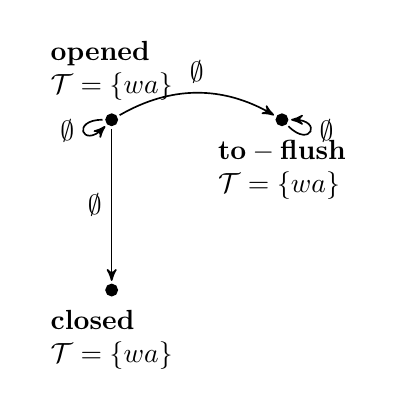
\begin{tikzpicture}[modal]
    \node[point] (to-flush) [label=90:{$\begin{array}{l}\mathbf{opened} \\ \mathcal{T}=\{wa\}\end{array}$}] {};
    \node[point] (opened) [right=of to-flush, label=270:{$\begin{array}{l}\mathbf{to-flush}\\\mathcal{T} = \{wa\} 
    \end{array}$}] {};
    \node[point](closed) [below=of to-flush, label=270:{$\begin{array}{l}\mathbf{closed}\\\mathcal{T} = \{wa\} 
    \end{array}$}] {};
    \path[->] (to-flush) edge[bend left] node[above]{$\emptyset$} (opened);
    \path[->] (opened) edge[reflexive right,out=-45,in=0,looseness=18] node[right] {$\emptyset$} (opened);
    \path[->] (to-flush) edge[reflexive left,out=180,in=225,looseness=18] node[left] {$\emptyset$} (to-flush);
     \path[->] (to-flush) edge node[left] {$\emptyset$} (closed);
\end{tikzpicture}
  %  \caption{Caption}
    \label{fig:enter-label}
\end{figure}
\column{.19\textwidth}
\begin{figure}
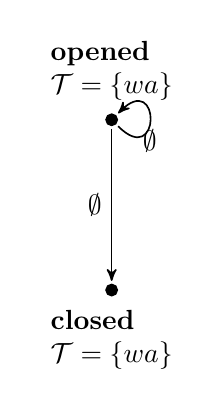
\begin{tikzpicture}[modal]
    \node[point] (opened) [label=above:{$\begin{array}{l}\mathbf{opened}\\ \mathcal{T}=\{wa\}\end{array}$}] {};
     \node[point](closed) [below=of opened, label=270:{$\begin{array}{l}\mathbf{closed}\\\mathcal{T} = \{wa\} 
    \end{array}$}] {};
    \path[->] (opened) edge[reflexive right,out=-45,in=45,looseness=18] node[below] {$\emptyset$} (opened);
      \path[->] (opened) edge node[left] {$\emptyset$} (closed);
\end{tikzpicture}
%    \caption{Caption}
    \label{fig:enter-label}
    \end{figure}
    \end{columns}
\end{frame}
\begin{frame}{We Need This}\scriptsize
\[
\inferrule[UpdIsl]{
        \alpha~\textrm{physically atomic}\\
        \forall s_0 \;\ldotp  \;((s;\mathsf{T})\;\overset{\mathsf{rely}^{*}}{\sqsubseteq}_\pi\;( s_0;\mathsf{T}))\; \vdash
        \triple{ \varphi(s_0)\ast P }{\alpha}{ \exists s' \;, \;\mathsf{T}'\;\ldotp \; (s_0;\mathsf{T})\; \overset{\mathsf{guar}^{*}}{\sqsubseteq}_\pi \;(s';\mathsf{T}') \ast 
        \varphi(s')\ast Q}
    }{
      \fbox{$\varphi$}^{\gamma}_{\pi} \vdash
      \triple{ \ownGhost{\gamma}{s;\mathsf{T}}_{\pi} \ast P }
            {\alpha}
        { \exists \; s', \mathsf{T}' \ldotp \ownGhost{\gamma}{s';\mathsf{T}'}_{\pi} \ast Q }
    }
\]
\[
\inferrule[Bisim]{
	\pi\sim\pi'\quad\quad 
	q\; \epsilon_{\mathcal{S}} \;s \quad\quad q' \; \epsilon_{\mathcal{S}} \;s' \\
	\triple{\ownGhost{\gamma}{s;\epsilon_{\overline{\mathcal{T}}}(\mathcal{T})}_{\pi'} \ast P}{C}{\ownGhost{\gamma}{s';\mathsf{T}'}_{\pi'} \ast Q}
}{
	\fbox{$\varphi$}^{\gamma}_{\pi} \vdash
    \triple{\ownGhost{\gamma}{q;\mathsf{T}}_{\pi}\ast P}{C}{\ownGhost{\gamma}{q';\mathsf{T}'}_{\pi} \ast Q}
}
\]
\end{frame}
\begin{frame}{How? Obligation - 2}\scriptsize
\[
\inferrule[UpdIsl]{
        \alpha~\textrm{physically atomic}\\
        \forall s_0 \;\ldotp  \;((s;\mathsf{T})\;\overset{\mathsf{rely}^{*}}{\sqsubseteq}_\pi\;( s_0;\mathsf{T}))\; \vdash
        \triple{ \varphi(s_0)\ast P }{\alpha}{ \exists s' \;, \;\mathsf{T}'\;\ldotp \; \tcbhighmath[boxrule=2pt,arc=1pt,colback=blue!10!white,colframe=blue,
  drop fuzzy shadow=red]{(s_0;\mathsf{T})\; \overset{\mathsf{guar}^{*}}{\sqsubseteq}_\pi \;(s';\mathsf{T}') } \ast 
        \varphi(s')\ast Q}
    }{
      \fbox{$\varphi$}^{\gamma}_{\pi} \vdash
      \triple{ \ownGhost{\gamma}{s;\mathsf{T}}_{\pi} \ast P }
            {\alpha}
        { \exists \; s', \mathsf{T}' \ldotp \ownGhost{\gamma}{s';\mathsf{T}'}_{\pi} \ast Q }
    }
\]
\[
\inferrule[Bisim]{
	\pi\sim\pi'\quad\quad 
	q\; \epsilon_{\mathcal{S}} \;s \quad\quad q' \; \epsilon_{\mathcal{S}} \;s' \\
	\triple{\ownGhost{\gamma}{s;\epsilon_{\overline{\mathcal{T}}}(\mathcal{T})}_{\pi'} \ast P}{C}{\ownGhost{\gamma}{s';\mathsf{T}'}_{\pi'} \ast Q}
}{
	\fbox{$\varphi$}^{\gamma}_{\pi} \vdash
    \triple{\ownGhost{\gamma}{q;\mathsf{T}}_{\pi}\ast P}{C}{\ownGhost{\gamma}{q';\mathsf{T}'}_{\pi} \ast Q}
}
\]
\end{frame}
\begin{frame}{The Law of Guarantee}\scriptsize
    \begin{theorem}[Guarantee Bisim without Invariants] 
\[
\begin{array}{l}
\forall_{q',q, T'} \ldotp 
    \epsilon_{\overline{\mathcal{T}}} ( T) \equiv T' \rightarrow \epsilon_{\mathcal{S}}(s,q)
\rightarrow   (q;T')\overset{\mathsf{rely}^{*}}{\sqsubseteq}_{\pi'}(q';T') \rightarrow  \\
\quad\quad\quad\quad \forall_{q'',T''}\ldotp (q';T')\overset{\mathsf{guar.}}{\sqsubseteq}_{\pi'}(q'';T'') \rightarrow  \\
\quad\quad\quad\quad\quad\quad \exists_{s',s'',T'_0,T''_0} \ldotp (s';T'_0) \overset{\mathsf{guar.}}{\sqsubseteq}_{\pi} (s'';T''_0) \land \\ \quad\quad\quad\quad\quad\quad\quad\quad \epsilon_{\mathcal{S}}(s')=q' \land \epsilon_{\mathcal{S}}(s'') = q'' \land \epsilon_{\overline{\mathcal{T}}}(T'_0) \equiv T' \land \epsilon_{\overline{\mathcal{T}}}(T''_0) \equiv T''
 \end{array}
\]
\end{theorem}
\begin{itemize}
    \item \emph{Under the embedded client interference}, the steps taken by the target STS must be countered by a one in the source STS
    \item From target STS to source STS
    \item Identifying the valid \emph{post} state 
\end{itemize}
\end{frame}
\begin{frame}{The Law of Guarantee}\scriptsize
    
\begin{figure}
% Gradient Info
  \scriptsize
\centering





% Gradient Info
  
\tikzset {_jj1caqhkd/.code = {\pgfsetadditionalshadetransform{ \pgftransformshift{\pgfpoint{0 bp } { 0 bp }  }  \pgftransformrotate{0 }  \pgftransformscale{2 }  }}}
\pgfdeclarehorizontalshading{_k63sulqoe}{150bp}{rgb(0bp)=(0.27,0.28,0.3);
rgb(37.5bp)=(0.27,0.28,0.3);
rgb(62.5bp)=(0,0,0);
rgb(100bp)=(0,0,0)}

% Gradient Info
  
\tikzset {_9fqc921fc/.code = {\pgfsetadditionalshadetransform{ \pgftransformshift{\pgfpoint{0 bp } { 0 bp }  }  \pgftransformrotate{0 }  \pgftransformscale{2 }  }}}
\pgfdeclarehorizontalshading{_sfbqmua1b}{150bp}{rgb(0bp)=(0.27,0.28,0.3);
rgb(37.5bp)=(0.27,0.28,0.3);
rgb(62.5bp)=(0,0,0);
rgb(100bp)=(0,0,0)}

% Gradient Info
  
\tikzset {_0uh9db9h5/.code = {\pgfsetadditionalshadetransform{ \pgftransformshift{\pgfpoint{0 bp } { 0 bp }  }  \pgftransformrotate{0 }  \pgftransformscale{2 }  }}}
\pgfdeclarehorizontalshading{_k793wksx7}{150bp}{rgb(0bp)=(0.27,0.28,0.3);
rgb(37.5bp)=(0.27,0.28,0.3);
rgb(62.5bp)=(0,0,0);
rgb(100bp)=(0,0,0)}

% Gradient Info
  
\tikzset {_n8bsq1qhs/.code = {\pgfsetadditionalshadetransform{ \pgftransformshift{\pgfpoint{0 bp } { 0 bp }  }  \pgftransformrotate{0 }  \pgftransformscale{2 }  }}}
\pgfdeclarehorizontalshading{_zrmrqqjtm}{150bp}{rgb(0bp)=(0.27,0.28,0.3);
rgb(37.5bp)=(0.27,0.28,0.3);
rgb(62.5bp)=(0,0,0);
rgb(100bp)=(0,0,0)}
\tikzset{every picture/.style={line width=0.75pt}} %set default line width to 0.75pt        

\begin{tikzpicture}[x=0.75pt,y=0.75pt,yscale=-0.7,xscale=0.7]
%uncomment if require: \path (0,393); %set diagram left start at 0, and has height of 393

%Shape: Circle [id:dp43870864910047014] 
\draw  [fill={rgb, 255:red, 0; green, 0; blue, 0 }  ,fill opacity=1 ] (305.95,298.38) .. controls (306.3,300.56) and (304.81,302.61) .. (302.62,302.95) .. controls (300.44,303.3) and (298.39,301.81) .. (298.05,299.62) .. controls (297.7,297.44) and (299.19,295.39) .. (301.38,295.05) .. controls (303.56,294.7) and (305.61,296.19) .. (305.95,298.38) -- cycle ;
%Curve Lines [id:da9888158968931531] 
\draw [color={rgb, 255:red, 0; green, 0; blue, 0 }  ,draw opacity=1 ]   (278.88,218.21) .. controls (225.98,197.33) and (221.67,119.63) .. (315.64,94.13) ;
\draw [shift={(315.64,94.13)}, rotate = 166.16] [color={rgb, 255:red, 0; green, 0; blue, 0 }  ,draw opacity=1 ][line width=0.75]    (0,5.59) -- (0,-5.59)(-5.03,5.59) -- (-5.03,-5.59)   ;
\draw [shift={(278.88,218.21)}, rotate = 197.1] [color={rgb, 255:red, 0; green, 0; blue, 0 }  ,draw opacity=1 ][line width=0.75]    (0,5.59) -- (0,-5.59)(-5.03,5.59) -- (-5.03,-5.59)   ;
%Straight Lines [id:da6126973711466699] 
\draw  [dash pattern={on 0.75pt off 0.75pt}]  (458.63,110.63) .. controls (460.19,112.4) and (460.09,114.06) .. (458.32,115.62) .. controls (456.55,117.18) and (456.45,118.84) .. (458.01,120.61) .. controls (459.57,122.38) and (459.47,124.04) .. (457.7,125.6) .. controls (455.93,127.16) and (455.83,128.82) .. (457.39,130.59) .. controls (458.96,132.36) and (458.86,134.02) .. (457.09,135.59) .. controls (455.32,137.15) and (455.22,138.81) .. (456.78,140.58) .. controls (458.34,142.35) and (458.24,144.01) .. (456.47,145.57) .. controls (454.7,147.13) and (454.6,148.79) .. (456.16,150.56) .. controls (457.72,152.33) and (457.62,153.99) .. (455.85,155.55) .. controls (454.08,157.11) and (453.98,158.77) .. (455.54,160.54) .. controls (457.1,162.31) and (457,163.97) .. (455.23,165.53) .. controls (453.46,167.09) and (453.36,168.75) .. (454.92,170.52) .. controls (456.48,172.29) and (456.38,173.95) .. (454.61,175.51) .. controls (452.84,177.07) and (452.74,178.73) .. (454.3,180.5) .. controls (455.86,182.27) and (455.76,183.93) .. (453.99,185.49) .. controls (452.22,187.05) and (452.12,188.71) .. (453.68,190.48) .. controls (455.24,192.25) and (455.14,193.91) .. (453.37,195.47) .. controls (451.6,197.03) and (451.5,198.69) .. (453.06,200.46) .. controls (454.62,202.23) and (454.52,203.89) .. (452.75,205.45) .. controls (450.98,207.01) and (450.88,208.67) .. (452.44,210.44) -- (452.32,212.38) -- (452.32,212.38) ;
%Straight Lines [id:da7211161672050015] 
\draw    (302,299) -- (302.51,250.37) ;
\draw [shift={(302.53,248.37)}, rotate = 90.6] [color={rgb, 255:red, 0; green, 0; blue, 0 }  ][line width=0.75]    (10.93,-3.29) .. controls (6.95,-1.4) and (3.31,-0.3) .. (0,0) .. controls (3.31,0.3) and (6.95,1.4) .. (10.93,3.29)   ;
%Curve Lines [id:da2226472034778313] 
\draw [color={rgb, 255:red, 0; green, 0; blue, 0 }  ,draw opacity=1 ]   (349.49,213.15) .. controls (308.98,187.97) and (307.96,149.19) .. (318.78,105.74) ;
\draw [shift={(318.78,105.74)}, rotate = 104.89] [color={rgb, 255:red, 0; green, 0; blue, 0 }  ,draw opacity=1 ][line width=0.75]    (0,5.59) -- (0,-5.59)(-5.03,5.59) -- (-5.03,-5.59)   ;
\draw [shift={(349.49,213.15)}, rotate = 209.03] [color={rgb, 255:red, 0; green, 0; blue, 0 }  ,draw opacity=1 ][line width=0.75]    (0,5.59) -- (0,-5.59)(-5.03,5.59) -- (-5.03,-5.59)   ;
%Straight Lines [id:da6718822924381407] 
\draw [line width=1.5]  [dash pattern={on 1.69pt off 2.76pt}]  (124,109) -- (172,109) ;
\draw [shift={(172,109)}, rotate = 0] [color={rgb, 255:red, 0; green, 0; blue, 0 }  ][line width=1.5]      (6.71,-6.71) .. controls (3.01,-6.71) and (0,-3.7) .. (0,0) .. controls (0,3.7) and (3.01,6.71) .. (6.71,6.71) ;
\draw [shift={(124,109)}, rotate = 180] [color={rgb, 255:red, 0; green, 0; blue, 0 }  ][line width=1.5]      (6.71,-6.71) .. controls (3.01,-6.71) and (0,-3.7) .. (0,0) .. controls (0,3.7) and (3.01,6.71) .. (6.71,6.71) ;
%Straight Lines [id:da6734208132149195] 
\draw  [dash pattern={on 0.75pt off 0.75pt}]  (195.56,121.23) .. controls (196.92,123.16) and (196.64,124.8) .. (194.71,126.15) .. controls (192.78,127.51) and (192.5,129.15) .. (193.85,131.08) .. controls (195.21,133.01) and (194.93,134.65) .. (193,136.01) .. controls (191.07,137.36) and (190.79,139) .. (192.14,140.93) .. controls (193.49,142.86) and (193.21,144.5) .. (191.28,145.86) .. controls (189.35,147.22) and (189.07,148.86) .. (190.43,150.79) .. controls (191.78,152.72) and (191.5,154.36) .. (189.57,155.71) .. controls (187.64,157.07) and (187.36,158.71) .. (188.72,160.64) .. controls (190.07,162.57) and (189.79,164.21) .. (187.86,165.56) .. controls (185.93,166.92) and (185.65,168.56) .. (187.01,170.49) .. controls (188.36,172.42) and (188.08,174.06) .. (186.15,175.42) .. controls (184.22,176.77) and (183.94,178.41) .. (185.29,180.34) .. controls (186.65,182.27) and (186.37,183.91) .. (184.44,185.27) .. controls (182.51,186.63) and (182.23,188.27) .. (183.58,190.2) .. controls (184.94,192.13) and (184.66,193.77) .. (182.73,195.12) .. controls (180.8,196.48) and (180.52,198.12) .. (181.87,200.05) .. controls (183.23,201.98) and (182.95,203.62) .. (181.02,204.97) .. controls (179.09,206.33) and (178.81,207.97) .. (180.16,209.9) .. controls (181.51,211.83) and (181.23,213.47) .. (179.3,214.83) .. controls (177.37,216.18) and (177.09,217.82) .. (178.45,219.75) .. controls (179.8,221.68) and (179.52,223.32) .. (177.59,224.68) .. controls (175.66,226.04) and (175.38,227.68) .. (176.74,229.61) .. controls (178.09,231.54) and (177.81,233.18) .. (175.88,234.53) .. controls (173.95,235.89) and (173.67,237.53) .. (175.03,239.46) .. controls (176.38,241.39) and (176.1,243.03) .. (174.17,244.38) .. controls (172.24,245.74) and (171.96,247.38) .. (173.32,249.31) .. controls (174.67,251.24) and (174.39,252.88) .. (172.46,254.24) .. controls (170.53,255.59) and (170.25,257.23) .. (171.6,259.16) -- (171.5,259.76) -- (171.5,259.76) ;
%Straight Lines [id:da14467646434184522] 
\draw  [dash pattern={on 0.75pt off 0.75pt}]  (82.75,119.12) .. controls (84.65,120.51) and (84.9,122.16) .. (83.51,124.06) .. controls (82.12,125.96) and (82.37,127.61) .. (84.27,129) .. controls (86.17,130.39) and (86.42,132.04) .. (85.03,133.94) .. controls (83.64,135.85) and (83.89,137.5) .. (85.8,138.89) .. controls (87.7,140.28) and (87.95,141.93) .. (86.56,143.83) .. controls (85.17,145.73) and (85.42,147.38) .. (87.32,148.77) .. controls (89.22,150.16) and (89.47,151.81) .. (88.08,153.71) .. controls (86.69,155.61) and (86.94,157.26) .. (88.84,158.65) .. controls (90.74,160.04) and (90.99,161.69) .. (89.6,163.59) .. controls (88.21,165.49) and (88.46,167.14) .. (90.36,168.54) .. controls (92.27,169.93) and (92.52,171.57) .. (91.13,173.48) .. controls (89.74,175.38) and (89.99,177.03) .. (91.89,178.42) .. controls (93.79,179.81) and (94.04,181.46) .. (92.65,183.36) .. controls (91.26,185.26) and (91.51,186.91) .. (93.41,188.3) .. controls (95.31,189.69) and (95.56,191.34) .. (94.17,193.24) .. controls (92.78,195.14) and (93.03,196.79) .. (94.93,198.19) .. controls (96.83,199.58) and (97.08,201.23) .. (95.69,203.13) .. controls (94.3,205.04) and (94.55,206.68) .. (96.46,208.07) .. controls (98.36,209.46) and (98.61,211.11) .. (97.22,213.01) .. controls (95.83,214.91) and (96.08,216.56) .. (97.98,217.95) .. controls (99.88,219.34) and (100.13,220.99) .. (98.74,222.89) .. controls (97.35,224.79) and (97.6,226.44) .. (99.5,227.84) .. controls (101.4,229.23) and (101.65,230.88) .. (100.26,232.78) .. controls (98.87,234.69) and (99.12,236.33) .. (101.03,237.72) .. controls (102.93,239.11) and (103.18,240.76) .. (101.79,242.66) .. controls (100.4,244.56) and (100.65,246.21) .. (102.55,247.6) .. controls (104.45,248.99) and (104.7,250.64) .. (103.31,252.54) .. controls (101.92,254.44) and (102.17,256.09) .. (104.07,257.49) .. controls (105.97,258.88) and (106.22,260.53) .. (104.83,262.43) -- (105.5,266.76) -- (105.5,266.76) ;
%Flowchart: Terminator [id:dp05466038201614887] 
\draw   (94.16,15) -- (417.84,15) .. controls (459.9,15) and (494,41.86) .. (494,75) .. controls (494,108.14) and (459.9,135) .. (417.84,135) -- (94.16,135) .. controls (52.1,135) and (18,108.14) .. (18,75) .. controls (18,41.86) and (52.1,15) .. (94.16,15) -- cycle ;
%Straight Lines [id:da646760238778985] 
\draw  [dash pattern={on 0.75pt off 0.75pt}]  (357.44,110.44) .. controls (359.25,111.93) and (359.41,113.59) .. (357.91,115.41) .. controls (356.41,117.22) and (356.57,118.88) .. (358.38,120.39) .. controls (360.19,121.9) and (360.35,123.56) .. (358.85,125.37) .. controls (357.35,127.18) and (357.51,128.84) .. (359.32,130.35) .. controls (361.13,131.85) and (361.29,133.51) .. (359.79,135.32) .. controls (358.29,137.13) and (358.45,138.79) .. (360.26,140.3) .. controls (362.08,141.8) and (362.24,143.46) .. (360.74,145.28) .. controls (359.24,147.09) and (359.4,148.75) .. (361.21,150.26) .. controls (363.02,151.76) and (363.18,153.42) .. (361.68,155.23) .. controls (360.18,157.04) and (360.34,158.7) .. (362.15,160.21) .. controls (363.96,161.72) and (364.12,163.38) .. (362.62,165.19) .. controls (361.12,167) and (361.28,168.66) .. (363.09,170.17) .. controls (364.91,171.67) and (365.07,173.33) .. (363.57,175.15) .. controls (362.07,176.96) and (362.23,178.62) .. (364.04,180.12) .. controls (365.85,181.63) and (366.01,183.29) .. (364.51,185.1) .. controls (363.01,186.91) and (363.17,188.57) .. (364.98,190.08) .. controls (366.79,191.59) and (366.95,193.25) .. (365.45,195.06) .. controls (363.95,196.87) and (364.11,198.53) .. (365.92,200.03) .. controls (367.74,201.53) and (367.9,203.19) .. (366.4,205.01) .. controls (364.9,206.82) and (365.06,208.48) .. (366.87,209.99) .. controls (368.68,211.5) and (368.84,213.16) .. (367.34,214.97) -- (367.66,218.37) -- (367.66,218.37) ;
%Curve Lines [id:da402851755809829] 
\draw    (127,296) .. controls (403.61,359.68) and (553.81,292.92) .. (453.85,240.04) ;
\draw [shift={(452.32,239.25)}, rotate = 27.23] [color={rgb, 255:red, 0; green, 0; blue, 0 }  ][line width=0.75]    (10.93,-3.29) .. controls (6.95,-1.4) and (3.31,-0.3) .. (0,0) .. controls (3.31,0.3) and (6.95,1.4) .. (10.93,3.29)   ;
%Curve Lines [id:da9384548899500653] 
\draw    (193,297) .. controls (186.81,319.63) and (576.56,344.44) .. (381.1,242.8) ;
\draw [shift={(381.1,242.8)}, rotate = 27.47] [color={rgb, 255:red, 0; green, 0; blue, 0 }  ][line width=0.75]    (10.93,-3.29) .. controls (6.95,-1.4) and (3.31,-0.3) .. (0,0) .. controls (3.31,0.3) and (6.95,1.4) .. (10.93,3.29)   ;
%Straight Lines [id:da27317164230230584] 
\draw [line width=1.5]  [dash pattern={on 1.69pt off 2.76pt}]  (371.5,106) -- (418.5,106) ;
\draw [shift={(418.5,106)}, rotate = 0] [color={rgb, 255:red, 0; green, 0; blue, 0 }  ][line width=1.5]      (6.71,-6.71) .. controls (3.01,-6.71) and (0,-3.7) .. (0,0) .. controls (0,3.7) and (3.01,6.71) .. (6.71,6.71) ;
\draw [shift={(371.5,106)}, rotate = 180] [color={rgb, 255:red, 0; green, 0; blue, 0 }  ][line width=1.5]      (6.71,-6.71) .. controls (3.01,-6.71) and (0,-3.7) .. (0,0) .. controls (0,3.7) and (3.01,6.71) .. (6.71,6.71) ;
%Curve Lines [id:da6244413086376972] 
\draw    (48,92) .. controls (10.19,11.4) and (320.37,53.57) .. (425.43,90.44) ;
\draw [shift={(427,91)}, rotate = 199.67] [color={rgb, 255:red, 0; green, 0; blue, 0 }  ][line width=0.75]    (10.93,-3.29) .. controls (6.95,-1.4) and (3.31,-0.3) .. (0,0) .. controls (3.31,0.3) and (6.95,1.4) .. (10.93,3.29)   ;
%Curve Lines [id:da2024567097605494] 
\draw    (168,91) .. controls (66.03,35.56) and (271.32,73.23) .. (321.53,84.66) ;
\draw [shift={(323,85)}, rotate = 193.04] [color={rgb, 255:red, 0; green, 0; blue, 0 }  ][line width=0.75]    (10.93,-3.29) .. controls (6.95,-1.4) and (3.31,-0.3) .. (0,0) .. controls (3.31,0.3) and (6.95,1.4) .. (10.93,3.29)   ;
%Shape: Regular Polygon [id:dp6148802272069613] 
\path  [shading=_k63sulqoe,_jj1caqhkd] (321.53,229.37) -- (315.97,242.8) -- (302.53,248.37) -- (289.1,242.8) -- (283.53,229.37) -- (289.1,215.93) -- (302.53,210.37) -- (315.97,215.93) -- cycle ; % for fading 
 \draw   (321.53,229.37) -- (315.97,242.8) -- (302.53,248.37) -- (289.1,242.8) -- (283.53,229.37) -- (289.1,215.93) -- (302.53,210.37) -- (315.97,215.93) -- cycle ; % for border 

%Shape: Regular Polygon [id:dp3436355559475792] 
\path  [shading=_sfbqmua1b,_9fqc921fc] (386.66,229.37) -- (381.1,242.8) -- (367.66,248.37) -- (354.23,242.8) -- (348.66,229.37) -- (354.23,215.93) -- (367.66,210.37) -- (381.1,215.93) -- cycle ; % for fading 
 \draw   (386.66,229.37) -- (381.1,242.8) -- (367.66,248.37) -- (354.23,242.8) -- (348.66,229.37) -- (354.23,215.93) -- (367.66,210.37) -- (381.1,215.93) -- cycle ; % for border 

%Shape: Regular Polygon [id:dp9465055730522687] 
\path  [shading=_k793wksx7,_0uh9db9h5] (457.89,225.81) -- (452.32,239.25) -- (438.89,244.81) -- (425.45,239.25) -- (419.89,225.81) -- (425.45,212.38) -- (438.89,206.81) -- (452.32,212.38) -- cycle ; % for fading 
 \draw   (457.89,225.81) -- (452.32,239.25) -- (438.89,244.81) -- (425.45,239.25) -- (419.89,225.81) -- (425.45,212.38) -- (438.89,206.81) -- (452.32,212.38) -- cycle ; % for border 

%Shape: Regular Polygon [id:dp3394005239623432] 
\draw  [fill={rgb, 255:red, 255; green, 255; blue, 255 }  ,fill opacity=1 ] (464.13,106.38) -- (458.63,119.63) -- (445.38,125.13) -- (432.12,119.63) -- (426.63,106.38) -- (432.12,93.12) -- (445.38,87.63) -- (458.63,93.12) -- cycle ;
%Shape: Regular Polygon [id:dp9494011810300369] 
\path  [shading=_zrmrqqjtm,_n8bsq1qhs] (363,106) -- (357.44,119.44) -- (344,125) -- (330.56,119.44) -- (325,106) -- (330.56,92.56) -- (344,87) -- (357.44,92.56) -- cycle ; % for fading 
 \draw   (363,106) -- (357.44,119.44) -- (344,125) -- (330.56,119.44) -- (325,106) -- (330.56,92.56) -- (344,87) -- (357.44,92.56) -- cycle ; % for border 

%Shape: Regular Polygon [id:dp8863869044054484] 
\draw  [color={rgb, 255:red, 0; green, 0; blue, 0 }  ,draw opacity=1 ][fill={rgb, 255:red, 255; green, 255; blue, 255 }  ,fill opacity=1 ] (115,109.5) -- (104.25,128.12) -- (82.75,128.12) -- (72,109.5) -- (82.75,90.88) -- (104.25,90.88) -- cycle ;
%Shape: Regular Polygon [id:dp44541542413755164] 
\draw  [color={rgb, 255:red, 0; green, 0; blue, 0 }  ,draw opacity=1 ][fill={rgb, 255:red, 255; green, 255; blue, 255 }  ,fill opacity=1 ] (228,111.5) -- (217.19,130.23) -- (195.56,130.23) -- (184.75,111.5) -- (195.56,92.77) -- (217.19,92.77) -- cycle ;
%Flowchart: Terminator [id:dp6249808143221018] 
\draw   (103.68,184) -- (425.32,184) .. controls (467.12,184) and (501,216.68) .. (501,257) .. controls (501,297.32) and (467.12,330) .. (425.32,330) -- (103.68,330) .. controls (61.88,330) and (28,297.32) .. (28,257) .. controls (28,216.68) and (61.88,184) .. (103.68,184) -- cycle ;
%Shape: Regular Polygon [id:dp254645070425094] 
\draw  [color={rgb, 255:red, 0; green, 0; blue, 0 }  ,draw opacity=1 ][fill={rgb, 255:red, 255; green, 255; blue, 255 }  ,fill opacity=1 ] (137.75,277.38) -- (127,296) -- (105.5,296) -- (94.75,277.38) -- (105.5,258.76) -- (127,258.76) -- cycle ;
%Shape: Regular Polygon [id:dp8316067504539726] 
\draw  [color={rgb, 255:red, 0; green, 0; blue, 0 }  ,draw opacity=1 ][fill={rgb, 255:red, 255; green, 255; blue, 255 }  ,fill opacity=1 ] (203.75,278.38) -- (193,297) -- (171.5,297) -- (160.75,278.38) -- (171.5,259.76) -- (193,259.76) -- cycle ;

% Text Node
\draw (191,21) node [anchor=north west][inner sep=0.75pt]  [font=\scriptsize] [align=left] {$\displaystyle \mathcal{T}( \pi )$};
% Text Node
\draw (318,21) node [anchor=north west][inner sep=0.75pt]  [font=\scriptsize] [align=left] {$\displaystyle \mathcal{T}( \pi ')$};
% Text Node
\draw (53,263) node [anchor=north west][inner sep=0.75pt]  [font=\scriptsize] [align=left] {$\displaystyle \mathcal{S}( \pi )$};
% Text Node
\draw (53,217) node [anchor=north west][inner sep=0.75pt]  [font=\scriptsize] [align=left] {$\displaystyle \mathcal{S}( \pi ')$};
% Text Node
\draw (323,297) node  [font=\scriptsize]  {$s$};
% Text Node
\draw (381,201) node  [font=\scriptsize]  {$q'$};
% Text Node
\draw (236,96) node  [font=\scriptsize]  {$T'_{0}$};
% Text Node
\draw (302,197) node  [font=\scriptsize]  {$q$};
% Text Node
\draw (432,196) node  [font=\scriptsize]  {$q''$};
% Text Node
\draw (290,274) node  [font=\scriptsize]  {$\epsilon_{\mathcal{S}}$};
% Text Node
\draw  [color={rgb, 255:red, 255; green, 255; blue, 255 }  ,draw opacity=1 ][fill={rgb, 255:red, 255; green, 255; blue, 255 }  ,fill opacity=1 ]  (261, 156) circle [x radius= 9.9, y radius= 12.73]   ;
\draw (253,146) node [anchor=north west][inner sep=0.75pt]  [font=\scriptsize] [align=left] {$\overset{\mathsf{rely}^{*}}{\sqsubseteq}_{\pi'}$};
% Text Node
\draw (369,86) node  [font=\scriptsize]  {$T'$};
% Text Node
\draw (461,81) node  [font=\scriptsize]  {$T''$};
% Text Node
\draw (118,63) node  [font=\scriptsize]  {$\epsilon_{\overline{\mathcal{T}}}$};
% Text Node
\draw (210,260) node  [font=\scriptsize]  {$s'$};
% Text Node
\draw (143,260) node  [font=\scriptsize]  {$s''$};
% Text Node
\draw (469,268) node  [font=\scriptsize]  {$\epsilon_{\mathcal{S}}$};
% Text Node
\draw  [color={rgb, 255:red, 255; green, 255; blue, 255 }  ,draw opacity=1 ][fill={rgb, 255:red, 255; green, 255; blue, 255 }  ,fill opacity=1 ]  (118, 155) circle [x radius= 9.9, y radius= 12.73]   ;
\draw (110,145) node [anchor=north west][inner sep=0.75pt]  [font=\scriptsize] [align=left] {$\overset{\mathsf{guar}^{*}}{\sqsubseteq}_{\pi}$};
% Text Node
\draw  [color={rgb, 255:red, 255; green, 255; blue, 255 }  ,draw opacity=1 ][fill={rgb, 255:red, 255; green, 255; blue, 255 }  ,fill opacity=1 ]  (379, 155) circle [x radius= 9.9, y radius= 12.73]   ;
\draw (371,145) node [anchor=north west][inner sep=0.75pt]  [font=\scriptsize] [align=left] {$\overset{\mathsf{guar}^{*}}{\sqsubseteq}_{\pi'}$};
% Text Node
\draw (410,276) node  [font=\scriptsize]  {$\epsilon_{\mathcal{S}}$};
% Text Node
\draw (437.12,95.12) node [anchor=north west][inner sep=0.75pt]  [font=\scriptsize,color={rgb, 255:red, 0; green, 0; blue, 0 }  ,opacity=1 ] [align=left] {n};
% Text Node
\draw (78.12,100.12) node [anchor=north west][inner sep=0.75pt]  [font=\scriptsize,color={rgb, 255:red, 0; green, 0; blue, 0 }  ,opacity=1 ] [align=left] {n+1};
% Text Node
\draw (192.12,102.12) node [anchor=north west][inner sep=0.75pt]  [font=\scriptsize,color={rgb, 255:red, 0; green, 0; blue, 0 }  ,opacity=1 ] [align=left] {n+1};
% Text Node
\draw (168.12,270.12) node [anchor=north west][inner sep=0.75pt]  [font=\scriptsize,color={rgb, 255:red, 0; green, 0; blue, 0 }  ,opacity=1 ] [align=left] {n+1};
% Text Node
\draw (101.12,269.12) node [anchor=north west][inner sep=0.75pt]  [font=\scriptsize,color={rgb, 255:red, 0; green, 0; blue, 0 }  ,opacity=1 ] [align=left] {n+1};


\end{tikzpicture}
    \caption{Embedding the Guarantee Steps of Target STS}
    \label{fig:enter-label}
\end{figure} 

\end{frame}
\begin{frame}{The Law of Guarantee for the Bisimulation Instance}\scriptsize
    
\begin{columns}
\column{0.58\textwidth}    
\begin{figure}
  \scriptsize



% Gradient Info
  
\tikzset {_lr538qk06/.code = {\pgfsetadditionalshadetransform{ \pgftransformshift{\pgfpoint{0 bp } { 0 bp }  }  \pgftransformrotate{0 }  \pgftransformscale{2 }  }}}
\pgfdeclarehorizontalshading{_661kcafi6}{150bp}{rgb(0bp)=(0.27,0.28,0.3);
rgb(37.5bp)=(0.27,0.28,0.3);
rgb(62.5bp)=(0,0,0);
rgb(100bp)=(0,0,0)}

% Gradient Info
  
\tikzset {_x3qr0her1/.code = {\pgfsetadditionalshadetransform{ \pgftransformshift{\pgfpoint{0 bp } { 0 bp }  }  \pgftransformrotate{0 }  \pgftransformscale{2 }  }}}
\pgfdeclarehorizontalshading{_7p2w1vnp7}{150bp}{rgb(0bp)=(0.27,0.28,0.3);
rgb(37.5bp)=(0.27,0.28,0.3);
rgb(62.5bp)=(0,0,0);
rgb(100bp)=(0,0,0)}

% Gradient Info
  
\tikzset {_zc06ne93s/.code = {\pgfsetadditionalshadetransform{ \pgftransformshift{\pgfpoint{0 bp } { 0 bp }  }  \pgftransformrotate{0 }  \pgftransformscale{2 }  }}}
\pgfdeclarehorizontalshading{_xtllwjaa8}{150bp}{rgb(0bp)=(0.27,0.28,0.3);
rgb(37.5bp)=(0.27,0.28,0.3);
rgb(62.5bp)=(0,0,0);
rgb(100bp)=(0,0,0)}

% Gradient Info
  
\tikzset {_dho4c2mau/.code = {\pgfsetadditionalshadetransform{ \pgftransformshift{\pgfpoint{0 bp } { 0 bp }  }  \pgftransformrotate{0 }  \pgftransformscale{2 }  }}}
\pgfdeclarehorizontalshading{_7fhd5s1x1}{150bp}{rgb(0bp)=(0.27,0.28,0.3);
rgb(37.5bp)=(0.27,0.28,0.3);
rgb(62.5bp)=(0,0,0);
rgb(100bp)=(0,0,0)}
\tikzset{every picture/.style={line width=0.75pt}} %set default line width to 0.75pt        

\begin{tikzpicture}[x=0.75pt,y=0.75pt,yscale=-0.7,xscale=0.7]
%uncomment if require: \path (0,393); %set diagram left start at 0, and has height of 393

%Shape: Circle [id:dp43870864910047014] 
\draw  [fill={rgb, 255:red, 0; green, 0; blue, 0 }  ,fill opacity=1 ] (304.95,332.38) .. controls (305.3,334.56) and (303.81,336.61) .. (301.62,336.95) .. controls (299.44,337.3) and (297.39,335.81) .. (297.05,333.62) .. controls (296.7,331.44) and (298.19,329.39) .. (300.38,329.05) .. controls (302.56,328.7) and (304.61,330.19) .. (304.95,332.38) -- cycle ;
%Curve Lines [id:da9888158968931531] 
\draw [color={rgb, 255:red, 0; green, 0; blue, 0 }  ,draw opacity=1 ]   (277.9,244.24) .. controls (225.5,224.19) and (229.15,159.77) .. (315.02,120.76) ;
\draw [shift={(315.02,120.76)}, rotate = 156.61] [color={rgb, 255:red, 0; green, 0; blue, 0 }  ,draw opacity=1 ][line width=0.75]    (0,5.59) -- (0,-5.59)(-5.03,5.59) -- (-5.03,-5.59)   ;
\draw [shift={(277.9,244.24)}, rotate = 197.1] [color={rgb, 255:red, 0; green, 0; blue, 0 }  ,draw opacity=1 ][line width=0.75]    (0,5.59) -- (0,-5.59)(-5.03,5.59) -- (-5.03,-5.59)   ;
%Straight Lines [id:da6126973711466699] 
\draw  [dash pattern={on 0.75pt off 0.75pt}]  (457.63,136.63) .. controls (459.2,138.39) and (459.11,140.06) .. (457.35,141.63) .. controls (455.59,143.2) and (455.49,144.86) .. (457.06,146.62) .. controls (458.63,148.38) and (458.53,150.04) .. (456.77,151.61) .. controls (455.01,153.18) and (454.91,154.84) .. (456.48,156.6) .. controls (458.05,158.36) and (457.96,160.02) .. (456.2,161.59) .. controls (454.44,163.16) and (454.34,164.82) .. (455.91,166.58) .. controls (457.48,168.34) and (457.38,170.01) .. (455.62,171.58) .. controls (453.86,173.15) and (453.77,174.81) .. (455.34,176.57) .. controls (456.91,178.33) and (456.81,179.99) .. (455.05,181.56) .. controls (453.29,183.13) and (453.19,184.79) .. (454.76,186.55) .. controls (456.33,188.31) and (456.24,189.97) .. (454.48,191.54) .. controls (452.72,193.11) and (452.62,194.77) .. (454.19,196.53) .. controls (455.76,198.29) and (455.66,199.96) .. (453.9,201.53) .. controls (452.14,203.1) and (452.04,204.76) .. (453.61,206.52) .. controls (455.18,208.28) and (455.09,209.94) .. (453.33,211.51) .. controls (451.57,213.08) and (451.47,214.74) .. (453.04,216.5) .. controls (454.61,218.26) and (454.51,219.92) .. (452.75,221.49) .. controls (450.99,223.06) and (450.9,224.72) .. (452.47,226.48) .. controls (454.04,228.24) and (453.94,229.91) .. (452.18,231.48) .. controls (450.42,233.05) and (450.32,234.71) .. (451.89,236.47) .. controls (453.46,238.23) and (453.36,239.89) .. (451.6,241.46) -- (451.32,246.38) -- (451.32,246.38) ;
%Straight Lines [id:da7211161672050015] 
\draw    (301,333) -- (301.51,284.37) ;
\draw [shift={(301.53,282.37)}, rotate = 90.6] [color={rgb, 255:red, 0; green, 0; blue, 0 }  ][line width=0.75]    (10.93,-3.29) .. controls (6.95,-1.4) and (3.31,-0.3) .. (0,0) .. controls (3.31,0.3) and (6.95,1.4) .. (10.93,3.29)   ;
%Curve Lines [id:da2226472034778313] 
\draw [color={rgb, 255:red, 0; green, 0; blue, 0 }  ,draw opacity=1 ]   (350.77,246.73) .. controls (297.82,222.29) and (298.53,174.59) .. (317.22,131.03) ;
\draw [shift={(317.22,131.03)}, rotate = 114.54] [color={rgb, 255:red, 0; green, 0; blue, 0 }  ,draw opacity=1 ][line width=0.75]    (0,5.59) -- (0,-5.59)(-5.03,5.59) -- (-5.03,-5.59)   ;
\draw [shift={(350.77,246.73)}, rotate = 202.13] [color={rgb, 255:red, 0; green, 0; blue, 0 }  ,draw opacity=1 ][line width=0.75]    (0,5.59) -- (0,-5.59)(-5.03,5.59) -- (-5.03,-5.59)   ;
%Straight Lines [id:da6718822924381407] 
\draw [line width=1.5]  [dash pattern={on 1.69pt off 2.76pt}]  (123,126) -- (171,126) ;
\draw [shift={(171,126)}, rotate = 0] [color={rgb, 255:red, 0; green, 0; blue, 0 }  ][line width=1.5]      (6.71,-6.71) .. controls (3.01,-6.71) and (0,-3.7) .. (0,0) .. controls (0,3.7) and (3.01,6.71) .. (6.71,6.71) ;
\draw [shift={(123,126)}, rotate = 180] [color={rgb, 255:red, 0; green, 0; blue, 0 }  ][line width=1.5]      (6.71,-6.71) .. controls (3.01,-6.71) and (0,-3.7) .. (0,0) .. controls (0,3.7) and (3.01,6.71) .. (6.71,6.71) ;
%Straight Lines [id:da6734208132149195] 
\draw  [dash pattern={on 0.75pt off 0.75pt}]  (194.56,147.23) .. controls (195.93,149.14) and (195.66,150.79) .. (193.75,152.16) .. controls (191.84,153.54) and (191.57,155.19) .. (192.94,157.1) .. controls (194.31,159.01) and (194.04,160.66) .. (192.13,162.03) .. controls (190.22,163.4) and (189.95,165.05) .. (191.32,166.96) .. controls (192.69,168.87) and (192.42,170.52) .. (190.51,171.9) .. controls (188.6,173.27) and (188.33,174.92) .. (189.7,176.83) .. controls (191.07,178.74) and (190.8,180.39) .. (188.89,181.77) .. controls (186.98,183.14) and (186.71,184.79) .. (188.08,186.7) .. controls (189.45,188.61) and (189.18,190.26) .. (187.27,191.63) .. controls (185.36,193.01) and (185.09,194.66) .. (186.46,196.57) .. controls (187.83,198.48) and (187.56,200.13) .. (185.65,201.5) .. controls (183.74,202.87) and (183.47,204.52) .. (184.84,206.43) .. controls (186.21,208.34) and (185.94,209.99) .. (184.03,211.37) .. controls (182.12,212.74) and (181.85,214.39) .. (183.22,216.3) .. controls (184.59,218.21) and (184.32,219.86) .. (182.41,221.24) .. controls (180.5,222.61) and (180.23,224.26) .. (181.6,226.17) .. controls (182.97,228.08) and (182.7,229.73) .. (180.79,231.1) .. controls (178.88,232.48) and (178.61,234.13) .. (179.98,236.04) .. controls (181.35,237.95) and (181.08,239.6) .. (179.17,240.97) .. controls (177.26,242.35) and (176.99,244) .. (178.36,245.91) .. controls (179.73,247.82) and (179.46,249.47) .. (177.55,250.84) .. controls (175.64,252.21) and (175.37,253.86) .. (176.74,255.77) .. controls (178.11,257.68) and (177.84,259.33) .. (175.93,260.71) .. controls (174.02,262.08) and (173.75,263.73) .. (175.12,265.64) .. controls (176.49,267.55) and (176.22,269.2) .. (174.31,270.58) .. controls (172.4,271.95) and (172.13,273.6) .. (173.5,275.51) .. controls (174.87,277.42) and (174.6,279.07) .. (172.69,280.44) .. controls (170.78,281.82) and (170.51,283.47) .. (171.88,285.38) .. controls (173.25,287.29) and (172.98,288.94) .. (171.07,290.31) -- (170.5,293.76) -- (170.5,293.76) ;
%Straight Lines [id:da14467646434184522] 
\draw  [dash pattern={on 0.75pt off 0.75pt}]  (81.75,145.12) .. controls (83.65,146.51) and (83.9,148.16) .. (82.51,150.06) .. controls (81.12,151.96) and (81.37,153.61) .. (83.27,155) .. controls (85.17,156.39) and (85.42,158.04) .. (84.03,159.94) .. controls (82.64,161.85) and (82.89,163.5) .. (84.8,164.89) .. controls (86.7,166.28) and (86.95,167.93) .. (85.56,169.83) .. controls (84.17,171.73) and (84.42,173.38) .. (86.32,174.77) .. controls (88.22,176.16) and (88.47,177.81) .. (87.08,179.71) .. controls (85.69,181.61) and (85.94,183.26) .. (87.84,184.65) .. controls (89.74,186.04) and (89.99,187.69) .. (88.6,189.59) .. controls (87.21,191.49) and (87.46,193.14) .. (89.36,194.54) .. controls (91.27,195.93) and (91.52,197.57) .. (90.13,199.48) .. controls (88.74,201.38) and (88.99,203.03) .. (90.89,204.42) .. controls (92.79,205.81) and (93.04,207.46) .. (91.65,209.36) .. controls (90.26,211.26) and (90.51,212.91) .. (92.41,214.3) .. controls (94.31,215.69) and (94.56,217.34) .. (93.17,219.24) .. controls (91.78,221.14) and (92.03,222.79) .. (93.93,224.19) .. controls (95.83,225.58) and (96.08,227.23) .. (94.69,229.13) .. controls (93.3,231.04) and (93.55,232.68) .. (95.46,234.07) .. controls (97.36,235.46) and (97.61,237.11) .. (96.22,239.01) .. controls (94.83,240.91) and (95.08,242.56) .. (96.98,243.95) .. controls (98.88,245.34) and (99.13,246.99) .. (97.74,248.89) .. controls (96.35,250.79) and (96.6,252.44) .. (98.5,253.84) .. controls (100.4,255.23) and (100.65,256.88) .. (99.26,258.78) .. controls (97.87,260.69) and (98.12,262.33) .. (100.03,263.72) .. controls (101.93,265.11) and (102.18,266.76) .. (100.79,268.66) .. controls (99.4,270.56) and (99.65,272.21) .. (101.55,273.6) .. controls (103.45,274.99) and (103.7,276.64) .. (102.31,278.54) .. controls (100.92,280.44) and (101.17,282.09) .. (103.07,283.49) .. controls (104.97,284.88) and (105.22,286.53) .. (103.83,288.43) -- (104.5,292.76) -- (104.5,292.76) ;
%Flowchart: Terminator [id:dp05466038201614887] 
\draw   (93.16,23.5) -- (416.84,23.5) .. controls (458.9,23.5) and (493,54.5) .. (493,92.75) .. controls (493,131) and (458.9,162) .. (416.84,162) -- (93.16,162) .. controls (51.1,162) and (17,131) .. (17,92.75) .. controls (17,54.5) and (51.1,23.5) .. (93.16,23.5) -- cycle ;
%Straight Lines [id:da646760238778985] 
\draw  [dash pattern={on 0.75pt off 0.75pt}]  (356.44,136.44) .. controls (358.25,137.93) and (358.41,139.59) .. (356.91,141.41) .. controls (355.41,143.22) and (355.57,144.88) .. (357.38,146.39) .. controls (359.19,147.9) and (359.35,149.56) .. (357.85,151.37) .. controls (356.35,153.18) and (356.51,154.84) .. (358.32,156.35) .. controls (360.13,157.85) and (360.29,159.51) .. (358.79,161.32) .. controls (357.29,163.13) and (357.45,164.79) .. (359.26,166.3) .. controls (361.08,167.8) and (361.24,169.46) .. (359.74,171.28) .. controls (358.24,173.09) and (358.4,174.75) .. (360.21,176.26) .. controls (362.02,177.76) and (362.18,179.42) .. (360.68,181.23) .. controls (359.18,183.04) and (359.34,184.7) .. (361.15,186.21) .. controls (362.96,187.72) and (363.12,189.38) .. (361.62,191.19) .. controls (360.12,193) and (360.28,194.66) .. (362.09,196.17) .. controls (363.91,197.67) and (364.07,199.33) .. (362.57,201.15) .. controls (361.07,202.96) and (361.23,204.62) .. (363.04,206.12) .. controls (364.85,207.63) and (365.01,209.29) .. (363.51,211.1) .. controls (362.01,212.91) and (362.17,214.57) .. (363.98,216.08) .. controls (365.79,217.59) and (365.95,219.25) .. (364.45,221.06) .. controls (362.95,222.87) and (363.11,224.53) .. (364.92,226.03) .. controls (366.74,227.53) and (366.9,229.19) .. (365.4,231.01) .. controls (363.9,232.82) and (364.06,234.48) .. (365.87,235.99) .. controls (367.68,237.5) and (367.84,239.16) .. (366.34,240.97) -- (366.66,244.37) -- (366.66,244.37) ;
%Curve Lines [id:da402851755809829] 
\draw    (126,330) .. controls (402.61,393.68) and (552.81,326.92) .. (452.85,274.04) ;
\draw [shift={(451.32,273.25)}, rotate = 27.23] [color={rgb, 255:red, 0; green, 0; blue, 0 }  ][line width=0.75]    (10.93,-3.29) .. controls (6.95,-1.4) and (3.31,-0.3) .. (0,0) .. controls (3.31,0.3) and (6.95,1.4) .. (10.93,3.29)   ;
%Curve Lines [id:da9384548899500653] 
\draw    (192,331) .. controls (185.81,353.63) and (575.56,378.44) .. (380.1,276.8) ;
\draw [shift={(380.1,276.8)}, rotate = 27.47] [color={rgb, 255:red, 0; green, 0; blue, 0 }  ][line width=0.75]    (10.93,-3.29) .. controls (6.95,-1.4) and (3.31,-0.3) .. (0,0) .. controls (3.31,0.3) and (6.95,1.4) .. (10.93,3.29)   ;
%Straight Lines [id:da27317164230230584] 
\draw [line width=1.5]  [dash pattern={on 1.69pt off 2.76pt}]  (370.5,123) -- (417.5,123) ;
\draw [shift={(417.5,123)}, rotate = 0] [color={rgb, 255:red, 0; green, 0; blue, 0 }  ][line width=1.5]      (6.71,-6.71) .. controls (3.01,-6.71) and (0,-3.7) .. (0,0) .. controls (0,3.7) and (3.01,6.71) .. (6.71,6.71) ;
\draw [shift={(370.5,123)}, rotate = 180] [color={rgb, 255:red, 0; green, 0; blue, 0 }  ][line width=1.5]      (6.71,-6.71) .. controls (3.01,-6.71) and (0,-3.7) .. (0,0) .. controls (0,3.7) and (3.01,6.71) .. (6.71,6.71) ;
%Curve Lines [id:da6244413086376972] 
\draw    (47,109) .. controls (9,28) and (246,36) .. (426,108) ;
\draw [shift={(426,108)}, rotate = 201.8] [color={rgb, 255:red, 0; green, 0; blue, 0 }  ][line width=0.75]    (10.93,-3.29) .. controls (6.95,-1.4) and (3.31,-0.3) .. (0,0) .. controls (3.31,0.3) and (6.95,1.4) .. (10.93,3.29)   ;
%Curve Lines [id:da2024567097605494] 
\draw    (167,108) .. controls (19.5,51.5) and (164.5,35.5) .. (322,102) ;
\draw [shift={(322,102)}, rotate = 202.89] [color={rgb, 255:red, 0; green, 0; blue, 0 }  ][line width=0.75]    (10.93,-3.29) .. controls (6.95,-1.4) and (3.31,-0.3) .. (0,0) .. controls (3.31,0.3) and (6.95,1.4) .. (10.93,3.29)   ;
%Shape: Regular Polygon [id:dp6148802272069613] 
\path  [shading=_661kcafi6,_lr538qk06] (320.53,263.37) -- (314.97,276.8) -- (301.53,282.37) -- (288.1,276.8) -- (282.53,263.37) -- (288.1,249.93) -- (301.53,244.37) -- (314.97,249.93) -- cycle ; % for fading 
 \draw   (320.53,263.37) -- (314.97,276.8) -- (301.53,282.37) -- (288.1,276.8) -- (282.53,263.37) -- (288.1,249.93) -- (301.53,244.37) -- (314.97,249.93) -- cycle ; % for border 

%Shape: Regular Polygon [id:dp3436355559475792] 
\path  [shading=_7p2w1vnp7,_x3qr0her1] (385.66,263.37) -- (380.1,276.8) -- (366.66,282.37) -- (353.23,276.8) -- (347.66,263.37) -- (353.23,249.93) -- (366.66,244.37) -- (380.1,249.93) -- cycle ; % for fading 
 \draw   (385.66,263.37) -- (380.1,276.8) -- (366.66,282.37) -- (353.23,276.8) -- (347.66,263.37) -- (353.23,249.93) -- (366.66,244.37) -- (380.1,249.93) -- cycle ; % for border 

%Shape: Regular Polygon [id:dp9465055730522687] 
\path  [shading=_xtllwjaa8,_zc06ne93s] (456.89,259.81) -- (451.32,273.25) -- (437.89,278.81) -- (424.45,273.25) -- (418.89,259.81) -- (424.45,246.38) -- (437.89,240.81) -- (451.32,246.38) -- cycle ; % for fading 
 \draw   (456.89,259.81) -- (451.32,273.25) -- (437.89,278.81) -- (424.45,273.25) -- (418.89,259.81) -- (424.45,246.38) -- (437.89,240.81) -- (451.32,246.38) -- cycle ; % for border 

%Shape: Regular Polygon [id:dp3394005239623432] 
\draw  [fill={rgb, 255:red, 255; green, 255; blue, 255 }  ,fill opacity=1 ] (463.13,123.38) -- (457.63,136.63) -- (444.38,142.13) -- (431.12,136.63) -- (425.63,123.38) -- (431.12,110.12) -- (444.38,104.63) -- (457.63,110.12) -- cycle ;
%Shape: Regular Polygon [id:dp9494011810300369] 
\path  [shading=_7fhd5s1x1,_dho4c2mau] (362,123) -- (356.44,136.44) -- (343,142) -- (329.56,136.44) -- (324,123) -- (329.56,109.56) -- (343,104) -- (356.44,109.56) -- cycle ; % for fading 
 \draw   (362,123) -- (356.44,136.44) -- (343,142) -- (329.56,136.44) -- (324,123) -- (329.56,109.56) -- (343,104) -- (356.44,109.56) -- cycle ; % for border 

%Shape: Regular Polygon [id:dp8863869044054484] 
\draw  [color={rgb, 255:red, 0; green, 0; blue, 0 }  ,draw opacity=1 ][fill={rgb, 255:red, 255; green, 255; blue, 255 }  ,fill opacity=1 ] (114,126.5) -- (103.25,145.12) -- (81.75,145.12) -- (71,126.5) -- (81.75,107.88) -- (103.25,107.88) -- cycle ;
%Shape: Regular Polygon [id:dp44541542413755164] 
\draw  [color={rgb, 255:red, 0; green, 0; blue, 0 }  ,draw opacity=1 ][fill={rgb, 255:red, 255; green, 255; blue, 255 }  ,fill opacity=1 ] (227,128.5) -- (216.19,147.23) -- (194.56,147.23) -- (183.75,128.5) -- (194.56,109.77) -- (216.19,109.77) -- cycle ;
%Flowchart: Terminator [id:dp6249808143221018] 
\draw   (102.68,218) -- (424.32,218) .. controls (466.12,218) and (500,250.68) .. (500,291) .. controls (500,331.32) and (466.12,364) .. (424.32,364) -- (102.68,364) .. controls (60.88,364) and (27,331.32) .. (27,291) .. controls (27,250.68) and (60.88,218) .. (102.68,218) -- cycle ;
%Shape: Regular Polygon [id:dp254645070425094] 
\draw  [color={rgb, 255:red, 0; green, 0; blue, 0 }  ,draw opacity=1 ][fill={rgb, 255:red, 255; green, 255; blue, 255 }  ,fill opacity=1 ] (136.75,311.38) -- (126,330) -- (104.5,330) -- (93.75,311.38) -- (104.5,292.76) -- (126,292.76) -- cycle ;
%Shape: Regular Polygon [id:dp8316067504539726] 
\draw  [color={rgb, 255:red, 0; green, 0; blue, 0 }  ,draw opacity=1 ][fill={rgb, 255:red, 255; green, 255; blue, 255 }  ,fill opacity=1 ] (202.75,312.38) -- (192,331) -- (170.5,331) -- (159.75,312.38) -- (170.5,293.76) -- (192,293.76) -- cycle ;
%Straight Lines [id:da3235170560956031] 
\draw    (175.5,88.5) -- (319.52,111.19) ;
\draw [shift={(321.5,111.5)}, rotate = 188.95] [color={rgb, 255:red, 0; green, 0; blue, 0 }  ][line width=0.75]    (10.93,-3.29) .. controls (6.95,-1.4) and (3.31,-0.3) .. (0,0) .. controls (3.31,0.3) and (6.95,1.4) .. (10.93,3.29)   ;
%Shape: Circle [id:dp762124246088761] 
\draw  [fill={rgb, 255:red, 0; green, 0; blue, 0 }  ,fill opacity=1 ] (169.5,85) .. controls (169.84,87.18) and (168.35,89.23) .. (166.17,89.57) .. controls (163.99,89.92) and (161.94,88.43) .. (161.6,86.25) .. controls (161.25,84.06) and (162.74,82.02) .. (164.93,81.67) .. controls (167.11,81.33) and (169.16,82.82) .. (169.5,85) -- cycle ;

% Text Node
\draw (193,29) node [anchor=north west][inner sep=0.75pt]  [font=\scriptsize] [align=left] {$\displaystyle \mathcal{T}( \pi )$};
% Text Node
\draw (331,29) node [anchor=north west][inner sep=0.75pt]  [font=\scriptsize] [align=left] {$\displaystyle \mathcal{T}( \pi ')$};
% Text Node
\draw (52,297) node [anchor=north west][inner sep=0.75pt]  [font=\scriptsize] [align=left] {$\displaystyle \mathcal{S}( \pi )$};
% Text Node
\draw (52,251) node [anchor=north west][inner sep=0.75pt]  [font=\scriptsize] [align=left] {$\displaystyle \mathcal{S}( \pi ')$};
% Text Node
\draw (328,331) node  [font=\scriptsize]  {$opened$};
% Text Node
\draw (55,123) node  [font=\scriptsize]  {$T''_{0}$};
% Text Node
\draw (380,235) node  [font=\scriptsize]  {$q'$};
% Text Node
\draw (235,113) node  [font=\scriptsize]  {$T'_{0}$};
% Text Node
\draw (301,231) node  [font=\scriptsize]  {$q$};
% Text Node
\draw (431,230) node  [font=\scriptsize]  {$q''$};
% Text Node
\draw (289,308) node  [font=\scriptsize]  {$\epsilon_{\mathcal{S}}$};
% Text Node
\draw  [color={rgb, 255:red, 255; green, 255; blue, 255 }  ,draw opacity=1 ][fill={rgb, 255:red, 255; green, 255; blue, 255 }  ,fill opacity=1 ]  (264, 194) circle [x radius= 9.9, y radius= 12.73]   ;
\draw (256,184) node [anchor=north west][inner sep=0.75pt]  [font=\scriptsize] [align=left] {$\overset{\mathsf{rely.}^{*}}{\sqsubseteq}_{\pi'}$};
% Text Node
\draw (368,103) node  [font=\scriptsize]  {$T'$};
% Text Node
\draw (460,98) node  [font=\scriptsize]  {$T''$};
% Text Node
\draw (95,80) node  [font=\scriptsize]  {$\epsilon_{\overline{\mathcal{T}}}$};
% Text Node
\draw (209,294) node  [font=\scriptsize]  {$s'$};
% Text Node
\draw (142,294) node  [font=\scriptsize]  {$s''$};
% Text Node
\draw (468,302) node  [font=\scriptsize]  {$\epsilon_{\mathcal{S}}$};
% Text Node
\draw  [color={rgb, 255:red, 255; green, 255; blue, 255 }  ,draw opacity=1 ][fill={rgb, 255:red, 255; green, 255; blue, 255 }  ,fill opacity=1 ]  (125, 194) circle [x radius= 9.9, y radius= 12.73]   ;
\draw (117,184) node [anchor=north west][inner sep=0.75pt]  [font=\scriptsize] [align=left] {$\overset{\mathsf{guar.}^{*}}{\sqsubseteq}_{\pi}$};
% Text Node
\draw  [color={rgb, 255:red, 255; green, 255; blue, 255 }  ,draw opacity=1 ][fill={rgb, 255:red, 255; green, 255; blue, 255 }  ,fill opacity=1 ]  (392, 194) circle [x radius= 9.9, y radius= 12.73]   ;
\draw (384,184) node [anchor=north west][inner sep=0.75pt]  [font=\scriptsize] [align=left] {$\overset{\mathsf{guar.}^{*}}{\sqsubseteq}_{\pi'}$};
% Text Node
\draw (409,310) node  [font=\scriptsize]  {$\epsilon_{\mathcal{S}}$};
% Text Node
\draw (55,52) node  [font=\scriptsize]  {$\epsilon_{\overline{\mathcal{T}}}$};
% Text Node
\draw (436.12,112.12) node [anchor=north west][inner sep=0.75pt]  [font=\scriptsize,color={rgb, 255:red, 0; green, 0; blue, 0 }  ,opacity=1 ] [align=left] {n};
% Text Node
\draw (77.12,117.12) node [anchor=north west][inner sep=0.75pt]  [font=\scriptsize,color={rgb, 255:red, 0; green, 0; blue, 0 }  ,opacity=1 ] [align=left] {n+1};
% Text Node
\draw (191.12,119.12) node [anchor=north west][inner sep=0.75pt]  [font=\scriptsize,color={rgb, 255:red, 0; green, 0; blue, 0 }  ,opacity=1 ] [align=left] {n+1};
% Text Node
\draw (167.12,304.12) node [anchor=north west][inner sep=0.75pt]  [font=\scriptsize,color={rgb, 255:red, 0; green, 0; blue, 0 }  ,opacity=1 ] [align=left] {n+1};
% Text Node
\draw (100.12,303.12) node [anchor=north west][inner sep=0.75pt]  [font=\scriptsize,color={rgb, 255:red, 0; green, 0; blue, 0 }  ,opacity=1 ] [align=left] {n+1};
% Text Node
\draw (166,72) node  [font=\scriptsize]  {$\emptyset $};
% Text Node
\draw (203,80) node  [font=\scriptsize]  {$\epsilon_{\overline{\mathcal{T}}}$};


\end{tikzpicture}
\end{figure}
\column{0.3\textwidth}
\begin{figure}\scriptsize
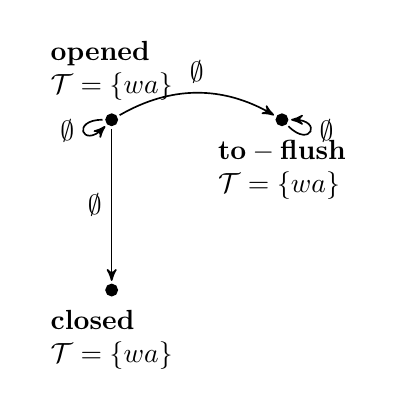
\begin{tikzpicture}[modal]
    \node[point] (to-flush) [label=90:{$\begin{array}{l}\mathbf{opened} \\ \mathcal{T}=\{wa\}\end{array}$}] {};
    \node[point] (opened) [right=of to-flush, label=270:{$\begin{array}{l}\mathbf{to-flush}\\\mathcal{T} = \{wa\} 
    \end{array}$}] {};
    \node[point](closed) [below=of to-flush, label=270:{$\begin{array}{l}\mathbf{closed}\\\mathcal{T} = \{wa\} 
    \end{array}$}] {};
    \path[->] (to-flush) edge[bend left] node[above]{$\emptyset$} (opened);
    \path[->] (opened) edge[reflexive right,out=-45,in=0,looseness=18] node[right] {$\emptyset$} (opened);
    \path[->] (to-flush) edge[reflexive left,out=180,in=225,looseness=18] node[left] {$\emptyset$} (to-flush);
     \path[->] (to-flush) edge node[left] {$\emptyset$} (closed);
\end{tikzpicture}
  %  \caption{Caption}
 %   \label{fig:enter-label}
\end{figure}
\column{.11\textwidth}
\begin{figure}
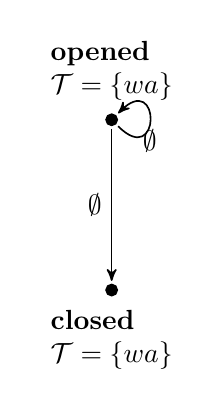
\begin{tikzpicture}[modal]
    \node[point] (opened) [label=above:{$\begin{array}{l}\mathbf{opened}\\ \mathcal{T}=\{wa\}\end{array}$}] {};
     \node[point](closed) [below=of opened, label=270:{$\begin{array}{l}\mathbf{closed}\\\mathcal{T} = \{wa\} 
    \end{array}$}] {};
    \path[->] (opened) edge[reflexive right,out=-45,in=45,looseness=18] node[below] {$\emptyset$} (opened);
      \path[->] (opened) edge node[left] {$\emptyset$} (closed);
\end{tikzpicture}
%    \caption{Caption}
  %  \label{fig:enter-label}
    \end{figure}
    \end{columns}
\end{frame}
\begin{frame}{The Law of Guarantee for the Bisimulation Instance}\scriptsize
    
\begin{columns}
\column{0.58\textwidth}    
\begin{figure}
  \scriptsize



% Gradient Info
  
\tikzset {_4bs8geb5j/.code = {\pgfsetadditionalshadetransform{ \pgftransformshift{\pgfpoint{0 bp } { 0 bp }  }  \pgftransformrotate{0 }  \pgftransformscale{2 }  }}}
\pgfdeclarehorizontalshading{_bawj7ymd1}{150bp}{rgb(0bp)=(0.27,0.28,0.3);
rgb(37.5bp)=(0.27,0.28,0.3);
rgb(62.5bp)=(0,0,0);
rgb(100bp)=(0,0,0)}

% Gradient Info
  
\tikzset {_v332v0wn3/.code = {\pgfsetadditionalshadetransform{ \pgftransformshift{\pgfpoint{0 bp } { 0 bp }  }  \pgftransformrotate{0 }  \pgftransformscale{2 }  }}}
\pgfdeclarehorizontalshading{_liwvvips9}{150bp}{rgb(0bp)=(0.27,0.28,0.3);
rgb(37.5bp)=(0.27,0.28,0.3);
rgb(62.5bp)=(0,0,0);
rgb(100bp)=(0,0,0)}

% Gradient Info
  
\tikzset {_xyfl2lkkh/.code = {\pgfsetadditionalshadetransform{ \pgftransformshift{\pgfpoint{0 bp } { 0 bp }  }  \pgftransformrotate{0 }  \pgftransformscale{2 }  }}}
\pgfdeclarehorizontalshading{_uw6ywtlyb}{150bp}{rgb(0bp)=(0.27,0.28,0.3);
rgb(37.5bp)=(0.27,0.28,0.3);
rgb(62.5bp)=(0,0,0);
rgb(100bp)=(0,0,0)}

% Gradient Info
  
\tikzset {_g59cot4l2/.code = {\pgfsetadditionalshadetransform{ \pgftransformshift{\pgfpoint{0 bp } { 0 bp }  }  \pgftransformrotate{0 }  \pgftransformscale{2 }  }}}
\pgfdeclarehorizontalshading{_66qjt1vaw}{150bp}{rgb(0bp)=(0.27,0.28,0.3);
rgb(37.5bp)=(0.27,0.28,0.3);
rgb(62.5bp)=(0,0,0);
rgb(100bp)=(0,0,0)}

% Gradient Info
  
\tikzset {_909rsdnoj/.code = {\pgfsetadditionalshadetransform{ \pgftransformshift{\pgfpoint{0 bp } { 0 bp }  }  \pgftransformrotate{0 }  \pgftransformscale{2 }  }}}
\pgfdeclarehorizontalshading{_pbbidlcsm}{150bp}{rgb(0bp)=(0.27,0.28,0.3);
rgb(37.5bp)=(0.27,0.28,0.3);
rgb(62.5bp)=(0,0,0);
rgb(100bp)=(0,0,0)}
\tikzset{every picture/.style={line width=0.75pt}} %set default line width to 0.75pt        

\begin{tikzpicture}[x=0.75pt,y=0.75pt,yscale=-0.7,xscale=0.7]
%uncomment if require: \path (0,393); %set diagram left start at 0, and has height of 393

%Shape: Circle [id:dp10374250889686953] 
\draw  [fill={rgb, 255:red, 0; green, 0; blue, 0 }  ,fill opacity=1 ] (281.95,341.38) .. controls (282.3,343.56) and (280.81,345.61) .. (278.62,345.95) .. controls (276.44,346.3) and (274.39,344.81) .. (274.05,342.62) .. controls (273.7,340.44) and (275.19,338.39) .. (277.38,338.05) .. controls (279.56,337.7) and (281.61,339.19) .. (281.95,341.38) -- cycle ;
%Straight Lines [id:da07625120306989985] 
\draw  [dash pattern={on 0.75pt off 0.75pt}]  (457.63,136.63) .. controls (459.2,138.39) and (459.11,140.06) .. (457.35,141.63) .. controls (455.59,143.2) and (455.49,144.86) .. (457.06,146.62) .. controls (458.63,148.38) and (458.53,150.04) .. (456.77,151.61) .. controls (455.01,153.18) and (454.91,154.84) .. (456.48,156.6) .. controls (458.05,158.36) and (457.96,160.02) .. (456.2,161.59) .. controls (454.44,163.16) and (454.34,164.82) .. (455.91,166.58) .. controls (457.48,168.34) and (457.38,170.01) .. (455.62,171.58) .. controls (453.86,173.15) and (453.77,174.81) .. (455.34,176.57) .. controls (456.91,178.33) and (456.81,179.99) .. (455.05,181.56) .. controls (453.29,183.13) and (453.19,184.79) .. (454.76,186.55) .. controls (456.33,188.31) and (456.24,189.97) .. (454.48,191.54) .. controls (452.72,193.11) and (452.62,194.77) .. (454.19,196.53) .. controls (455.76,198.29) and (455.66,199.96) .. (453.9,201.53) .. controls (452.14,203.1) and (452.04,204.76) .. (453.61,206.52) .. controls (455.18,208.28) and (455.09,209.94) .. (453.33,211.51) .. controls (451.57,213.08) and (451.47,214.74) .. (453.04,216.5) .. controls (454.61,218.26) and (454.51,219.92) .. (452.75,221.49) .. controls (450.99,223.06) and (450.9,224.72) .. (452.47,226.48) .. controls (454.04,228.24) and (453.94,229.91) .. (452.18,231.48) .. controls (450.42,233.05) and (450.32,234.71) .. (451.89,236.47) .. controls (453.46,238.23) and (453.36,239.89) .. (451.6,241.46) -- (451.32,246.38) -- (451.32,246.38) ;
%Straight Lines [id:da6002418923236006] 
\draw    (277.5,331.5) -- (277.02,285) ;
\draw [shift={(277,283)}, rotate = 89.41] [color={rgb, 255:red, 0; green, 0; blue, 0 }  ][line width=0.75]    (10.93,-3.29) .. controls (6.95,-1.4) and (3.31,-0.3) .. (0,0) .. controls (3.31,0.3) and (6.95,1.4) .. (10.93,3.29)   ;
%Straight Lines [id:da6415540969153894] 
\draw [line width=1.5]  [dash pattern={on 1.69pt off 2.76pt}]  (123,126) -- (171,126) ;
\draw [shift={(171,126)}, rotate = 0] [color={rgb, 255:red, 0; green, 0; blue, 0 }  ][line width=1.5]      (6.71,-6.71) .. controls (3.01,-6.71) and (0,-3.7) .. (0,0) .. controls (0,3.7) and (3.01,6.71) .. (6.71,6.71) ;
\draw [shift={(123,126)}, rotate = 180] [color={rgb, 255:red, 0; green, 0; blue, 0 }  ][line width=1.5]      (6.71,-6.71) .. controls (3.01,-6.71) and (0,-3.7) .. (0,0) .. controls (0,3.7) and (3.01,6.71) .. (6.71,6.71) ;
%Straight Lines [id:da14452474248555403] 
\draw  [dash pattern={on 0.75pt off 0.75pt}]  (194.56,147.23) .. controls (195.93,149.14) and (195.66,150.79) .. (193.75,152.16) .. controls (191.84,153.54) and (191.57,155.19) .. (192.94,157.1) .. controls (194.31,159.01) and (194.04,160.66) .. (192.13,162.03) .. controls (190.22,163.4) and (189.95,165.05) .. (191.32,166.96) .. controls (192.69,168.87) and (192.42,170.52) .. (190.51,171.9) .. controls (188.6,173.27) and (188.33,174.92) .. (189.7,176.83) .. controls (191.07,178.74) and (190.8,180.39) .. (188.89,181.77) .. controls (186.98,183.14) and (186.71,184.79) .. (188.08,186.7) .. controls (189.45,188.61) and (189.18,190.26) .. (187.27,191.63) .. controls (185.36,193.01) and (185.09,194.66) .. (186.46,196.57) .. controls (187.83,198.48) and (187.56,200.13) .. (185.65,201.5) .. controls (183.74,202.87) and (183.47,204.52) .. (184.84,206.43) .. controls (186.21,208.34) and (185.94,209.99) .. (184.03,211.37) .. controls (182.12,212.74) and (181.85,214.39) .. (183.22,216.3) .. controls (184.59,218.21) and (184.32,219.86) .. (182.41,221.24) .. controls (180.5,222.61) and (180.23,224.26) .. (181.6,226.17) .. controls (182.97,228.08) and (182.7,229.73) .. (180.79,231.1) .. controls (178.88,232.48) and (178.61,234.13) .. (179.98,236.04) .. controls (181.35,237.95) and (181.08,239.6) .. (179.17,240.97) .. controls (177.26,242.35) and (176.99,244) .. (178.36,245.91) .. controls (179.73,247.82) and (179.46,249.47) .. (177.55,250.84) .. controls (175.64,252.21) and (175.37,253.86) .. (176.74,255.77) .. controls (178.11,257.68) and (177.84,259.33) .. (175.93,260.71) .. controls (174.02,262.08) and (173.75,263.73) .. (175.12,265.64) .. controls (176.49,267.55) and (176.22,269.2) .. (174.31,270.58) .. controls (172.4,271.95) and (172.13,273.6) .. (173.5,275.51) .. controls (174.87,277.42) and (174.6,279.07) .. (172.69,280.44) .. controls (170.78,281.82) and (170.51,283.47) .. (171.88,285.38) .. controls (173.25,287.29) and (172.98,288.94) .. (171.07,290.31) -- (170.5,293.76) -- (170.5,293.76) ;
%Straight Lines [id:da5656199530045085] 
\draw  [dash pattern={on 0.75pt off 0.75pt}]  (81.75,145.12) .. controls (83.65,146.51) and (83.9,148.16) .. (82.51,150.06) .. controls (81.12,151.96) and (81.37,153.61) .. (83.27,155) .. controls (85.17,156.39) and (85.42,158.04) .. (84.03,159.94) .. controls (82.64,161.85) and (82.89,163.5) .. (84.8,164.89) .. controls (86.7,166.28) and (86.95,167.93) .. (85.56,169.83) .. controls (84.17,171.73) and (84.42,173.38) .. (86.32,174.77) .. controls (88.22,176.16) and (88.47,177.81) .. (87.08,179.71) .. controls (85.69,181.61) and (85.94,183.26) .. (87.84,184.65) .. controls (89.74,186.04) and (89.99,187.69) .. (88.6,189.59) .. controls (87.21,191.49) and (87.46,193.14) .. (89.36,194.54) .. controls (91.27,195.93) and (91.52,197.57) .. (90.13,199.48) .. controls (88.74,201.38) and (88.99,203.03) .. (90.89,204.42) .. controls (92.79,205.81) and (93.04,207.46) .. (91.65,209.36) .. controls (90.26,211.26) and (90.51,212.91) .. (92.41,214.3) .. controls (94.31,215.69) and (94.56,217.34) .. (93.17,219.24) .. controls (91.78,221.14) and (92.03,222.79) .. (93.93,224.19) .. controls (95.83,225.58) and (96.08,227.23) .. (94.69,229.13) .. controls (93.3,231.04) and (93.55,232.68) .. (95.46,234.07) .. controls (97.36,235.46) and (97.61,237.11) .. (96.22,239.01) .. controls (94.83,240.91) and (95.08,242.56) .. (96.98,243.95) .. controls (98.88,245.34) and (99.13,246.99) .. (97.74,248.89) .. controls (96.35,250.79) and (96.6,252.44) .. (98.5,253.84) .. controls (100.4,255.23) and (100.65,256.88) .. (99.26,258.78) .. controls (97.87,260.69) and (98.12,262.33) .. (100.03,263.72) .. controls (101.93,265.11) and (102.18,266.76) .. (100.79,268.66) .. controls (99.4,270.56) and (99.65,272.21) .. (101.55,273.6) .. controls (103.45,274.99) and (103.7,276.64) .. (102.31,278.54) .. controls (100.92,280.44) and (101.17,282.09) .. (103.07,283.49) .. controls (104.97,284.88) and (105.22,286.53) .. (103.83,288.43) -- (104.5,292.76) -- (104.5,292.76) ;
%Flowchart: Terminator [id:dp5142419597085324] 
\draw   (93.16,23.5) -- (416.84,23.5) .. controls (458.9,23.5) and (493,54.5) .. (493,92.75) .. controls (493,131) and (458.9,162) .. (416.84,162) -- (93.16,162) .. controls (51.1,162) and (17,131) .. (17,92.75) .. controls (17,54.5) and (51.1,23.5) .. (93.16,23.5) -- cycle ;
%Curve Lines [id:da3060130276973776] 
\draw    (126,330) .. controls (366.29,401.14) and (545.7,330.22) .. (466.71,264.49) ;
\draw [shift={(465.5,263.5)}, rotate = 38.83] [color={rgb, 255:red, 0; green, 0; blue, 0 }  ][line width=0.75]    (10.93,-3.29) .. controls (6.95,-1.4) and (3.31,-0.3) .. (0,0) .. controls (3.31,0.3) and (6.95,1.4) .. (10.93,3.29)   ;
%Curve Lines [id:da428030458846987] 
\draw    (192,331) .. controls (172.5,367.5) and (561.5,375.5) .. (406.53,277.37) ;
\draw [shift={(406.53,277.37)}, rotate = 32.34] [color={rgb, 255:red, 0; green, 0; blue, 0 }  ][line width=0.75]    (10.93,-3.29) .. controls (6.95,-1.4) and (3.31,-0.3) .. (0,0) .. controls (3.31,0.3) and (6.95,1.4) .. (10.93,3.29)   ;
%Straight Lines [id:da0908251053296587] 
\draw [line width=1.5]  [dash pattern={on 1.69pt off 2.76pt}]  (370.5,123) -- (417.5,123) ;
\draw [shift={(417.5,123)}, rotate = 0] [color={rgb, 255:red, 0; green, 0; blue, 0 }  ][line width=1.5]      (6.71,-6.71) .. controls (3.01,-6.71) and (0,-3.7) .. (0,0) .. controls (0,3.7) and (3.01,6.71) .. (6.71,6.71) ;
\draw [shift={(370.5,123)}, rotate = 180] [color={rgb, 255:red, 0; green, 0; blue, 0 }  ][line width=1.5]      (6.71,-6.71) .. controls (3.01,-6.71) and (0,-3.7) .. (0,0) .. controls (0,3.7) and (3.01,6.71) .. (6.71,6.71) ;
%Curve Lines [id:da7532522352524396] 
\draw    (47,109) .. controls (9,28) and (246,36) .. (426,108) ;
\draw [shift={(426,108)}, rotate = 201.8] [color={rgb, 255:red, 0; green, 0; blue, 0 }  ][line width=0.75]    (10.93,-3.29) .. controls (6.95,-1.4) and (3.31,-0.3) .. (0,0) .. controls (3.31,0.3) and (6.95,1.4) .. (10.93,3.29)   ;
%Curve Lines [id:da7544453249834986] 
\draw    (167,108) .. controls (19.5,51.5) and (164.5,35.5) .. (322,102) ;
\draw [shift={(322,102)}, rotate = 202.89] [color={rgb, 255:red, 0; green, 0; blue, 0 }  ][line width=0.75]    (10.93,-3.29) .. controls (6.95,-1.4) and (3.31,-0.3) .. (0,0) .. controls (3.31,0.3) and (6.95,1.4) .. (10.93,3.29)   ;
%Shape: Regular Polygon [id:dp20136629703946562] 
\path  [shading=_bawj7ymd1,_4bs8geb5j] (468.89,259.81) -- (463.32,273.25) -- (449.89,278.81) -- (436.45,273.25) -- (430.89,259.81) -- (436.45,246.38) -- (449.89,240.81) -- (463.32,246.38) -- cycle ; % for fading 
 \draw   (468.89,259.81) -- (463.32,273.25) -- (449.89,278.81) -- (436.45,273.25) -- (430.89,259.81) -- (436.45,246.38) -- (449.89,240.81) -- (463.32,246.38) -- cycle ; % for border 

%Shape: Regular Polygon [id:dp2786420024204732] 
\draw  [fill={rgb, 255:red, 255; green, 255; blue, 255 }  ,fill opacity=1 ] (463.13,123.38) -- (457.63,136.63) -- (444.38,142.13) -- (431.12,136.63) -- (425.63,123.38) -- (431.12,110.12) -- (444.38,104.63) -- (457.63,110.12) -- cycle ;
%Shape: Regular Polygon [id:dp33664108950971827] 
\path  [shading=_liwvvips9,_v332v0wn3] (362,123) -- (356.44,136.44) -- (343,142) -- (329.56,136.44) -- (324,123) -- (329.56,109.56) -- (343,104) -- (356.44,109.56) -- cycle ; % for fading 
 \draw   (362,123) -- (356.44,136.44) -- (343,142) -- (329.56,136.44) -- (324,123) -- (329.56,109.56) -- (343,104) -- (356.44,109.56) -- cycle ; % for border 

%Shape: Regular Polygon [id:dp2940478745108046] 
\draw  [color={rgb, 255:red, 0; green, 0; blue, 0 }  ,draw opacity=1 ][fill={rgb, 255:red, 255; green, 255; blue, 255 }  ,fill opacity=1 ] (114,126.5) -- (103.25,145.12) -- (81.75,145.12) -- (71,126.5) -- (81.75,107.88) -- (103.25,107.88) -- cycle ;
%Shape: Regular Polygon [id:dp5045566094380931] 
\draw  [color={rgb, 255:red, 0; green, 0; blue, 0 }  ,draw opacity=1 ][fill={rgb, 255:red, 255; green, 255; blue, 255 }  ,fill opacity=1 ] (227,128.5) -- (216.19,147.23) -- (194.56,147.23) -- (183.75,128.5) -- (194.56,109.77) -- (216.19,109.77) -- cycle ;
%Flowchart: Terminator [id:dp23019384616368277] 
\draw   (102.68,218) -- (424.32,218) .. controls (466.12,218) and (500,250.68) .. (500,291) .. controls (500,331.32) and (466.12,364) .. (424.32,364) -- (102.68,364) .. controls (60.88,364) and (27,331.32) .. (27,291) .. controls (27,250.68) and (60.88,218) .. (102.68,218) -- cycle ;
%Shape: Regular Polygon [id:dp6154837521257459] 
\draw  [color={rgb, 255:red, 0; green, 0; blue, 0 }  ,draw opacity=1 ][fill={rgb, 255:red, 255; green, 255; blue, 255 }  ,fill opacity=1 ] (136.75,311.38) -- (126,330) -- (104.5,330) -- (93.75,311.38) -- (104.5,292.76) -- (126,292.76) -- cycle ;
%Shape: Regular Polygon [id:dp863121896616676] 
\draw  [color={rgb, 255:red, 0; green, 0; blue, 0 }  ,draw opacity=1 ][fill={rgb, 255:red, 255; green, 255; blue, 255 }  ,fill opacity=1 ] (202.75,312.38) -- (192,331) -- (170.5,331) -- (159.75,312.38) -- (170.5,293.76) -- (192,293.76) -- cycle ;
%Straight Lines [id:da4794380943522847] 
\draw    (175.5,88.5) -- (319.52,111.19) ;
\draw [shift={(321.5,111.5)}, rotate = 188.95] [color={rgb, 255:red, 0; green, 0; blue, 0 }  ][line width=0.75]    (10.93,-3.29) .. controls (6.95,-1.4) and (3.31,-0.3) .. (0,0) .. controls (3.31,0.3) and (6.95,1.4) .. (10.93,3.29)   ;
%Shape: Circle [id:dp6767525726281827] 
\draw  [fill={rgb, 255:red, 0; green, 0; blue, 0 }  ,fill opacity=1 ] (169.5,85) .. controls (169.84,87.18) and (168.35,89.23) .. (166.17,89.57) .. controls (163.99,89.92) and (161.94,88.43) .. (161.6,86.25) .. controls (161.25,84.06) and (162.74,82.02) .. (164.93,81.67) .. controls (167.11,81.33) and (169.16,82.82) .. (169.5,85) -- cycle ;
%Curve Lines [id:da3464609398066154] 
\draw [color={rgb, 255:red, 0; green, 0; blue, 0 }  ,draw opacity=1 ]   (271.21,240.22) .. controls (172.61,234.85) and (221.06,91.62) .. (319.47,121.51) ;
\draw [shift={(319.47,121.51)}, rotate = 199.43] [color={rgb, 255:red, 0; green, 0; blue, 0 }  ,draw opacity=1 ][line width=0.75]    (0,5.59) -- (0,-5.59)(-5.03,5.59) -- (-5.03,-5.59)   ;
\draw [shift={(271.21,240.22)}, rotate = 179.74] [color={rgb, 255:red, 0; green, 0; blue, 0 }  ,draw opacity=1 ][line width=0.75]    (0,5.59) -- (0,-5.59)(-5.03,5.59) -- (-5.03,-5.59)   ;
%Shape: Regular Polygon [id:dp33983633461625784] 
\path  [shading=_uw6ywtlyb,_xyfl2lkkh] (296.53,259.37) -- (290.97,272.8) -- (277.53,278.37) -- (264.1,272.8) -- (258.53,259.37) -- (264.1,245.93) -- (277.53,240.37) -- (290.97,245.93) -- cycle ; % for fading 
 \draw   (296.53,259.37) -- (290.97,272.8) -- (277.53,278.37) -- (264.1,272.8) -- (258.53,259.37) -- (264.1,245.93) -- (277.53,240.37) -- (290.97,245.93) -- cycle ; % for border 

%Shape: Regular Polygon [id:dp8165294971663364] 
\path  [shading=_66qjt1vaw,_g59cot4l2] (369.53,259.37) -- (363.97,272.8) -- (350.53,278.37) -- (337.1,272.8) -- (331.53,259.37) -- (337.1,245.93) -- (350.53,240.37) -- (363.97,245.93) -- cycle ; % for fading 
 \draw   (369.53,259.37) -- (363.97,272.8) -- (350.53,278.37) -- (337.1,272.8) -- (331.53,259.37) -- (337.1,245.93) -- (350.53,240.37) -- (363.97,245.93) -- cycle ; % for border 

%Curve Lines [id:da47236597496369437] 
\draw [color={rgb, 255:red, 0; green, 0; blue, 0 }  ,draw opacity=1 ]   (328.35,247.29) .. controls (264.07,217.8) and (249.97,137.51) .. (319.63,123.76) ;
\draw [shift={(319.63,123.76)}, rotate = 171.45] [color={rgb, 255:red, 0; green, 0; blue, 0 }  ,draw opacity=1 ][line width=0.75]    (0,5.59) -- (0,-5.59)(-5.03,5.59) -- (-5.03,-5.59)   ;
\draw [shift={(328.35,247.29)}, rotate = 201.8] [color={rgb, 255:red, 0; green, 0; blue, 0 }  ,draw opacity=1 ][line width=0.75]    (0,5.59) -- (0,-5.59)(-5.03,5.59) -- (-5.03,-5.59)   ;
%Curve Lines [id:da03294131129754052] 
\draw [color={rgb, 255:red, 0; green, 0; blue, 0 }  ,draw opacity=1 ]   (387.84,242.71) .. controls (334.64,219.18) and (326.55,184.77) .. (341.31,146.21) ;
\draw [shift={(341.31,146.21)}, rotate = 112.86] [color={rgb, 255:red, 0; green, 0; blue, 0 }  ,draw opacity=1 ][line width=0.75]    (0,5.59) -- (0,-5.59)(-5.03,5.59) -- (-5.03,-5.59)   ;
\draw [shift={(387.84,242.71)}, rotate = 202.13] [color={rgb, 255:red, 0; green, 0; blue, 0 }  ,draw opacity=1 ][line width=0.75]    (0,5.59) -- (0,-5.59)(-5.03,5.59) -- (-5.03,-5.59)   ;
%Straight Lines [id:da6147928168538614] 
\draw  [dash pattern={on 0.75pt off 0.75pt}]  (352.44,136.44) .. controls (354.73,136.97) and (355.61,138.39) .. (355.08,140.68) .. controls (354.55,142.97) and (355.43,144.39) .. (357.72,144.92) .. controls (360.01,145.46) and (360.89,146.88) .. (360.36,149.17) .. controls (359.83,151.46) and (360.71,152.88) .. (363,153.41) .. controls (365.3,153.94) and (366.18,155.36) .. (365.65,157.66) .. controls (365.12,159.95) and (366,161.37) .. (368.29,161.9) .. controls (370.58,162.44) and (371.46,163.86) .. (370.93,166.15) .. controls (370.4,168.44) and (371.28,169.86) .. (373.57,170.39) .. controls (375.86,170.93) and (376.74,172.35) .. (376.21,174.64) .. controls (375.68,176.93) and (376.57,178.35) .. (378.86,178.88) .. controls (381.15,179.42) and (382.03,180.84) .. (381.5,183.13) .. controls (380.97,185.42) and (381.85,186.84) .. (384.14,187.37) .. controls (386.43,187.91) and (387.31,189.33) .. (386.78,191.62) .. controls (386.25,193.91) and (387.13,195.33) .. (389.42,195.86) .. controls (391.72,196.39) and (392.6,197.81) .. (392.07,200.11) .. controls (391.54,202.4) and (392.42,203.82) .. (394.71,204.35) .. controls (397,204.89) and (397.88,206.31) .. (397.35,208.6) .. controls (396.82,210.89) and (397.7,212.31) .. (399.99,212.84) .. controls (402.29,213.37) and (403.17,214.79) .. (402.64,217.09) .. controls (402.11,219.38) and (402.99,220.8) .. (405.28,221.33) .. controls (407.57,221.87) and (408.45,223.29) .. (407.92,225.58) .. controls (407.39,227.87) and (408.27,229.29) .. (410.56,229.82) .. controls (412.85,230.36) and (413.73,231.78) .. (413.2,234.07) .. controls (412.67,236.36) and (413.56,237.78) .. (415.85,238.31) .. controls (418.14,238.85) and (419.02,240.27) .. (418.49,242.56) -- (419.97,244.93) -- (419.97,244.93) ;
%Shape: Regular Polygon [id:dp410826442833196] 
\path  [shading=_pbbidlcsm,_909rsdnoj] (425.53,258.37) -- (419.97,271.8) -- (406.53,277.37) -- (393.1,271.8) -- (387.53,258.37) -- (393.1,244.93) -- (406.53,239.37) -- (419.97,244.93) -- cycle ; % for fading 
 \draw   (425.53,258.37) -- (419.97,271.8) -- (406.53,277.37) -- (393.1,271.8) -- (387.53,258.37) -- (393.1,244.93) -- (406.53,239.37) -- (419.97,244.93) -- cycle ; % for border 


% Text Node
\draw (193,29) node [anchor=north west][inner sep=0.75pt]  [font=\scriptsize] [align=left] {$\displaystyle \mathcal{T}( \pi )$};
% Text Node
\draw (331,29) node [anchor=north west][inner sep=0.75pt]  [font=\scriptsize] [align=left] {$\displaystyle \mathcal{T}( \pi ')$};
% Text Node
\draw (52,297) node [anchor=north west][inner sep=0.75pt]  [font=\scriptsize] [align=left] {$\displaystyle \mathcal{S}( \pi )$};
% Text Node
\draw (52,251) node [anchor=north west][inner sep=0.75pt]  [font=\scriptsize] [align=left] {$\displaystyle \mathcal{S}( \pi ')$};
% Text Node
\draw (305,339) node  [font=\scriptsize]  {$opened$};
% Text Node
\draw (55,123) node  [font=\scriptsize]  {$T''_{0}$};
% Text Node
\draw (235,113) node  [font=\scriptsize]  {$T'_{0}$};
% Text Node
\draw (443,230) node  [font=\scriptsize]  {$q''$};
% Text Node
\draw (266,311) node  [font=\scriptsize]  {$\epsilon_{\mathcal{S}}$};
% Text Node
\draw (368,103) node  [font=\scriptsize]  {$T'$};
% Text Node
\draw (460,98) node  [font=\scriptsize]  {$T''$};
% Text Node
\draw (95,80) node  [font=\scriptsize]  {$\epsilon_{\overline{\mathcal{T}}}$};
% Text Node
\draw (209,294) node  [font=\scriptsize]  {$s'$};
% Text Node
\draw (142,294) node  [font=\scriptsize]  {$s''$};
% Text Node
\draw (474,301) node  [font=\scriptsize]  {$\epsilon_{\mathcal{S}}$};
% Text Node
\draw  [color={rgb, 255:red, 255; green, 255; blue, 255 }  ,draw opacity=1 ][fill={rgb, 255:red, 255; green, 255; blue, 255 }  ,fill opacity=1 ]  (125, 189) circle [x radius= 9.9, y radius= 12.73]   ;
\draw (117,179) node [anchor=north west][inner sep=0.75pt]  [font=\scriptsize] [align=left] {$\overset{\mathsf{guar}^{*}}{\sqsubseteq}_{\pi}$};
% Text Node
\draw  [color={rgb, 255:red, 255; green, 255; blue, 255 }  ,draw opacity=1 ][fill={rgb, 255:red, 255; green, 255; blue, 255 }  ,fill opacity=1 ]  (408, 189) circle [x radius= 9.9, y radius= 12.73]   ;
\draw (400,179) node [anchor=north west][inner sep=0.75pt]  [font=\scriptsize] [align=left] {$\overset{\mathsf{guar}^{*}}{\sqsubseteq}_{\pi'}$};
% Text Node
\draw (417,312) node  [font=\scriptsize]  {$\epsilon_{\mathcal{S}}$};
% Text Node
\draw (55,52) node  [font=\scriptsize]  {$\epsilon_{\overline{\mathcal{T}}}$};
% Text Node
\draw (436.12,112.12) node [anchor=north west][inner sep=0.75pt]  [font=\scriptsize,color={rgb, 255:red, 0; green, 0; blue, 0 }  ,opacity=1 ] [align=left] {n};
% Text Node
\draw (77.12,117.12) node [anchor=north west][inner sep=0.75pt]  [font=\scriptsize,color={rgb, 255:red, 0; green, 0; blue, 0 }  ,opacity=1 ] [align=left] {n+1};
% Text Node
\draw (191.12,119.12) node [anchor=north west][inner sep=0.75pt]  [font=\scriptsize,color={rgb, 255:red, 0; green, 0; blue, 0 }  ,opacity=1 ] [align=left] {n+1};
% Text Node
\draw (167.12,304.12) node [anchor=north west][inner sep=0.75pt]  [font=\scriptsize,color={rgb, 255:red, 0; green, 0; blue, 0 }  ,opacity=1 ] [align=left] {n+1};
% Text Node
\draw (100.12,303.12) node [anchor=north west][inner sep=0.75pt]  [font=\scriptsize,color={rgb, 255:red, 0; green, 0; blue, 0 }  ,opacity=1 ] [align=left] {n+1};
% Text Node
\draw (166,72) node  [font=\scriptsize]  {$\emptyset $};
% Text Node
\draw (203,80) node  [font=\scriptsize]  {$\epsilon_{\overline{\mathcal{T}}}$};
% Text Node
\draw (305,294) node  [font=\scriptsize]  {$ \begin{array}{l}
x=\\
opened
\end{array}$};
% Text Node
\draw  [color={rgb, 255:red, 255; green, 255; blue, 255 }  ,draw opacity=1 ][fill={rgb, 255:red, 255; green, 255; blue, 255 }  ,fill opacity=1 ]  (291, 190) circle [x radius= 9.9, y radius= 12.73]   ;
\draw (283,180) node [anchor=north west][inner sep=0.75pt]  [font=\scriptsize] [align=left] {$\overset{\mathsf{rely}^{*}}{\sqsubseteq}_{\pi'}$};
% Text Node
\draw  [color={rgb, 255:red, 255; green, 255; blue, 255 }  ,draw opacity=1 ][fill={rgb, 255:red, 255; green, 255; blue, 255 }  ,fill opacity=1 ]  (240, 190) circle [x radius= 9.9, y radius= 12.73]   ;
\draw (232,180) node [anchor=north west][inner sep=0.75pt]  [font=\scriptsize] [align=left] {$\overset{\mathsf{rely}}{\sqsubseteq}_{\pi'}$};
% Text Node
\draw (334,230) node  [font=\scriptsize]  {$y$};
% Text Node
\draw (398,229) node  [font=\scriptsize]  {$z$};


\end{tikzpicture}
\end{figure}
\column{0.3\textwidth}
\begin{figure}\scriptsize
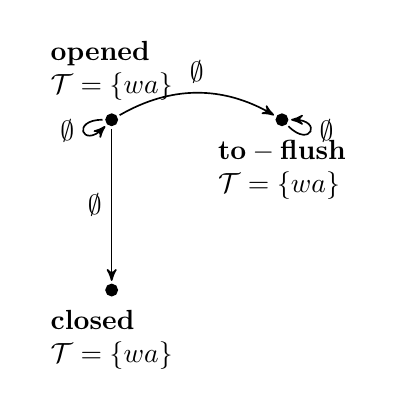
\begin{tikzpicture}[modal]
    \node[point] (to-flush) [label=90:{$\begin{array}{l}\mathbf{opened} \\ \mathcal{T}=\{wa\}\end{array}$}] {};
    \node[point] (opened) [right=of to-flush, label=270:{$\begin{array}{l}\mathbf{to-flush}\\\mathcal{T} = \{wa\} 
    \end{array}$}] {};
    \node[point](closed) [below=of to-flush, label=270:{$\begin{array}{l}\mathbf{closed}\\\mathcal{T} = \{wa\} 
    \end{array}$}] {};
    \path[->] (to-flush) edge[bend left] node[above]{$\emptyset$} (opened);
    \path[->] (opened) edge[reflexive right,out=-45,in=0,looseness=18] node[right] {$\emptyset$} (opened);
    \path[->] (to-flush) edge[reflexive left,out=180,in=225,looseness=18] node[left] {$\emptyset$} (to-flush);
     \path[->] (to-flush) edge node[left] {$\emptyset$} (closed);
\end{tikzpicture}
  %  \caption{Caption}
 %   \label{fig:enter-label}
\end{figure}
\column{.11\textwidth}
\begin{figure}
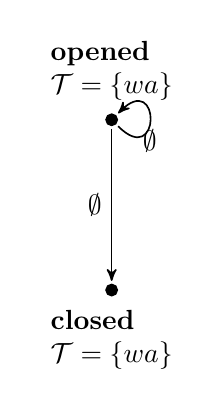
\begin{tikzpicture}[modal]
    \node[point] (opened) [label=above:{$\begin{array}{l}\mathbf{opened}\\ \mathcal{T}=\{wa\}\end{array}$}] {};
     \node[point](closed) [below=of opened, label=270:{$\begin{array}{l}\mathbf{closed}\\\mathcal{T} = \{wa\} 
    \end{array}$}] {};
    \path[->] (opened) edge[reflexive right,out=-45,in=45,looseness=18] node[below] {$\emptyset$} (opened);
      \path[->] (opened) edge node[left] {$\emptyset$} (closed);
\end{tikzpicture}
%    \caption{Caption}
  %  \label{fig:enter-label}
    \end{figure}
    \end{columns}
\end{frame}
\subsection{Invariants}
\begin{frame}{We Need This} \scriptsize
\[
\inferrule[UpdIsl]{
        \alpha~\textrm{physically atomic}\\
        \forall s_0 \;\ldotp  \;((s;\mathsf{T})\;\overset{\mathsf{rely}^{*}}{\sqsubseteq}_\pi\;( s_0;\mathsf{T}))\; \vdash
        \triple{ \varphi(s_0)\ast P }{\alpha}{ \exists s' \;, \;\mathsf{T}'\;\ldotp \; (s_0;\mathsf{T})\; \overset{\mathsf{guar}^{*}}{\sqsubseteq}_\pi \;(s';\mathsf{T}') \ast 
        \varphi(s')\ast Q}
    }{
      \fbox{$\varphi$}^{\gamma}_{\pi} \vdash
      \triple{ \ownGhost{\gamma}{s;\mathsf{T}}_{\pi} \ast P }
            {\alpha}
        { \exists \; s', \mathsf{T}' \ldotp \ownGhost{\gamma}{s';\mathsf{T}'}_{\pi} \ast Q }
    }
\]
\[
\inferrule[Bisim]{
	\pi\sim\pi'\quad\quad 
	q\; \epsilon_{\mathcal{S}} \;s \quad\quad q' \; \epsilon_{\mathcal{S}} \;s' \\
	\triple{\ownGhost{\gamma}{s;\epsilon_{\overline{\mathcal{T}}}(\mathcal{T})}_{\pi'} \ast P}{C}{\ownGhost{\gamma}{s';\mathsf{T}'}_{\pi'}\ast Q}
}{
	\fbox{$\varphi$}^{\gamma}_{\pi} \vdash
    \triple{\ownGhost{\gamma}{q;\mathsf{T}}_{\pi}\ast P}{C}{\ownGhost{\gamma}{q';\mathsf{T}'}_{\pi} \ast Q}
}
\]
\end{frame}
\begin{frame}{How? Obligation - 3} \scriptsize
\[
\inferrule[UpdIsl]{
        \alpha~\textrm{physically atomic}\\
        \forall s_0 \;\ldotp  \;((s;\mathsf{T})\;\overset{\mathsf{rely}^{*}}{\sqsubseteq}_\pi\;( s_0;\mathsf{T}))\; \vdash
        \triple{ \tcbhighmath[boxrule=2pt,arc=1pt,colback=blue!10!white,colframe=blue,
  drop fuzzy shadow=red]{\varphi(s_0)}\ast P }{\alpha}{ \exists s' \;, \;\mathsf{T}'\;\ldotp \; (s_0;\mathsf{T})\; \overset{\mathsf{guar}^{*}}{\sqsubseteq}_\pi \;(s';\mathsf{T}')  \ast 
        \varphi(s')\ast Q}
    }{
      \fbox{$\varphi$}^{\gamma}_{\pi} \vdash
      \triple{ \ownGhost{\gamma}{s;\mathsf{T}}_{\pi} \ast P }
            {\alpha}
        { \exists \; s', \mathsf{T}' \ldotp \ownGhost{\gamma}{s';\mathsf{T}'}_{\pi} \ast Q }
    }
\]
\[
\inferrule[Bisim]{
	\pi\sim\pi'\quad\quad 
	q\; \epsilon_{\mathcal{S}} \;s \quad\quad q' \; \epsilon_{\mathcal{S}} \;s' \\
	\triple{\ownGhost{\gamma}{s;\epsilon_{\overline{\mathcal{T}}}(\mathcal{T})}_{\pi'} \ast P}{C}{\ownGhost{\gamma}{s';\mathsf{T}'}_{\pi'} \ast Q}
}{
	\fbox{$\varphi$}^{\gamma}_{\pi} \vdash
    \triple{\ownGhost{\gamma}{q;\mathsf{T}}_{\pi}\ast P}{C}{\ownGhost{\gamma}{q';\mathsf{T}'}_{\pi} \ast Q}
}
\]
\end{frame}
\begin{frame}{How? Obligation - 4} \scriptsize
\[
\inferrule[UpdIsl]{
        \alpha~\textrm{physically atomic}\\
        \forall s_0 \;\ldotp  \;((s;\mathsf{T})\;\overset{\mathsf{rely}^{*}}{\sqsubseteq}_\pi\;( s_0;\mathsf{T}))\; \vdash
        \triple{ \tcbhighmath[boxrule=2pt,arc=1pt,colback=blue!10!white,colframe=blue,
  drop fuzzy shadow=red]{\varphi(s_0)}\ast P }{\alpha}{ \exists s' \;, \;\mathsf{T}'\;\ldotp \; (s_0;\mathsf{T})\; \overset{\mathsf{guar}^{*}}{\sqsubseteq}_\pi \;(s';\mathsf{T}')  \ast 
      \tcbhighmath[boxrule=2pt,arc=1pt,colback=blue!10!white,colframe=blue,
  drop fuzzy shadow=red]{  \varphi(s')}\ast Q}
    }{
      \fbox{$\varphi$}^{\gamma}_{\pi} \vdash
      \triple{ \ownGhost{\gamma}{s;\mathsf{T}}_{\pi} \ast P }
            {\alpha}
        { \exists \; s', \mathsf{T}' \ldotp \ownGhost{\gamma}{s';\mathsf{T}'}_{\pi}\ast Q }
    }
\]
\[
\inferrule[Bisim]{
	\pi\sim\pi'\quad\quad 
	q\; \epsilon_{\mathcal{S}} \;s \quad\quad q' \; \epsilon_{\mathcal{S}} \;s' \\
	\triple{\ownGhost{\gamma}{s;\epsilon_{\overline{\mathcal{T}}}(\mathcal{T})}_{\pi'} \ast P}{C}{\ownGhost{\gamma}{s';\mathsf{T}'}_{\pi'} \ast Q}
}{
	\fbox{$\varphi$}^{\gamma}_{\pi} \vdash
    \triple{\ownGhost{\gamma}{q;\mathsf{T}}_{\pi}\ast P}{C}{\ownGhost{\gamma}{q';\mathsf{T}'}_{\pi} \ast Q}
}
\]
\end{frame}
\begin{frame}{How? Intuition on Invariants in Bisimulation} \scriptsize
\[
\inferrule[UpdIsl]{
        \alpha~\textrm{physically atomic}\\
        \forall s_0 \;\ldotp  \;((s;\mathsf{T})\;\overset{\mathsf{rely}^{*}}{\sqsubseteq}_\pi\;( s_0;\mathsf{T}))\; \vdash
        \triple{ \tcbhighmath[boxrule=2pt,arc=1pt,colback=blue!10!white,colframe=blue,
  drop fuzzy shadow=red]{\varphi(s_0)}\ast P }{\alpha}{ \exists s' \;, \;\mathsf{T}'\;\ldotp \; (s_0;\mathsf{T})\; \overset{\mathsf{guar}^{*}}{\sqsubseteq}_\pi \;(s';\mathsf{T}')  \ast 
      \tcbhighmath[boxrule=2pt,arc=1pt,colback=blue!10!white,colframe=blue,
  drop fuzzy shadow=red]{  \varphi(s')}\ast Q}
    }{
      \fbox{$\varphi$}^{\gamma}_{\pi} \vdash
      \triple{ \ownGhost{\gamma}{s;\mathsf{T}} \ast P }
            {\alpha}
        { \exists \; s', \mathsf{T}' \ldotp \ownGhost{\gamma}{s';\mathsf{T}'}_{\pi} \ast Q }
    }
\]
\[
\inferrule[Bisim]{
	\pi\sim\pi'\quad\quad 
	q\; \epsilon_{\mathcal{S}} \;s \quad\quad q' \; \epsilon_{\mathcal{S}} \;s' \\
	\triple{\ownGhost{\gamma}{s;\epsilon_{\overline{\mathcal{T}}}(\mathcal{T})}_{\pi'} \ast P}{C}{\ownGhost{\gamma}{s';\mathsf{T}'}_{\pi'} \ast Q}
}{
	\fbox{$\varphi$}^{\gamma}_{\pi} \vdash
    \triple{\ownGhost{\gamma}{q;\mathsf{T}}_{\pi}\ast P}{C}{\ownGhost{\gamma}{q';\mathsf{T}'}_{\mathsf{\pi}} \ast Q}
}
\]
\begin{itemize}
    \item The post condition of the target state machine $\pi'$ implies the post condition of the source state machine $\pi$, e.g., \textsf{opened} 
    \item Applying \textsc{UpdIsl} would give 
    \begin{itemize}\scriptsize
        \item $\varphi'(\epsilon_{\mathcal{S}}(s0)) \;\vdash \;\exists \;s'\; \ldotp \varphi'(s')$ 
        \item \text{\scriptsize and precondition in the source STS} -- $\varphi(s0)$
        \end{itemize}
    \item To obtain $\exists\; s' \;\ldotp \;\varphi(s')$
\end{itemize}
\end{frame}
\begin{frame}{Invariants of File Protocols} \scriptsize
\begin{definition}[File Protocol Invariants]    
    \[
\varphi_{\mathsf{distributedfile}} \;(\;\ell\;, \;\mathsf{R}\;)( \;s \; )\;\triangleq \;
\left\{
\begin{array}{cc}
\mathsf{match}\; \mathsf{s} \; \mathsf{with}\\
  \mathsf{to-flush} \Rightarrow  &  \mathsf{R} \ast \exists \; \mathsf{fs} \ldotp \mathsf{isValidDirty}(\mathsf{fs}) \ast \\ & \quad\quad\quad\quad \ell \mapsto (\mathsf{fs}.id,\mathsf{fs}.\mathsf{status}=\mathsf{dirty})  \\
   \mathsf{opened} \Rightarrow  &  \mathsf{R} \ast \exists \; \mathsf{fs} \ldotp \mathsf{isValid}(\mathsf{fs}) \ast \\ & \quad\quad\quad\quad \ell \mapsto (\mathsf{fs}.id,\mathsf{fs}.\mathsf{status}=\mathsf{clean}) \\
   \mathsf{closed} \Rightarrow  & \exists \; \mathsf{fs} \ldotp \mathsf{isValidClosed}(\mathsf{fs}) \ast \\ & \quad\quad\quad\quad \ell \mapsto (\mathsf{fs}.id,\mathsf{fs}.\mathsf{status}=\textsf{closed}) 
\end{array}
\right\}
\]
\[
\varphi_{\mathsf{file}} \;(\;\ell \;\mathsf{R}\;)( \;s \;)\; \triangleq \;
\left\{
\begin{array}{cc}
\mathsf{match}\; \mathsf{s} \; \mathsf{with}\\
   \mathsf{opened} \Rightarrow  &  \mathsf{R} \ast \exists \; \mathsf{fs} \ldotp \mathsf{isValid}(\mathsf{fs}) \ast \ell \mapsto (\mathsf{fs}.id,\mathsf{fs}.\mathsf{status}=\mathsf{clean} \lor \mathsf{dirty}) \\
   \mathsf{closed} \Rightarrow  & \exists \; \mathsf{fs} \ldotp \mathsf{isValidClosed}(\mathsf{fs}) \ast \ell \mapsto (\mathsf{fs}.id,\mathsf{fs}.\mathsf{status}=\mathsf{closed}) 
\end{array}
\right\}
\]
\end{definition}
\end{frame}
\begin{frame}{The Law of Tolerance}\scriptsize
    \begin{columns}
        \column{0.5\textwidth}
        \begin{figure} \scriptsize
            \centering



\tikzset{every picture/.style={line width=0.75pt}} %set default line width to 0.75pt        

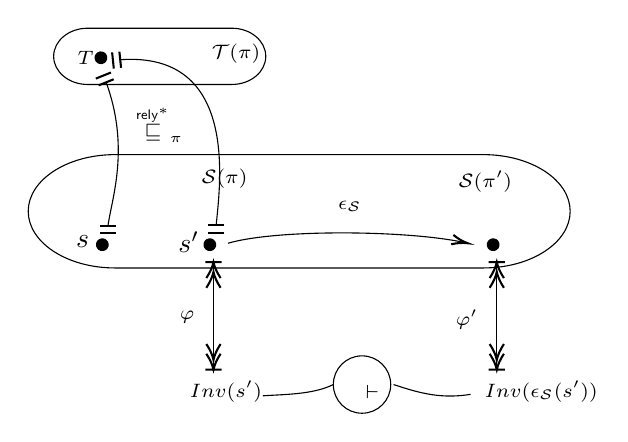
\begin{tikzpicture}[x=0.75pt,y=0.75pt,yscale=-0.7,xscale=0.7]
%uncomment if require: \path (0,1468); %set diagram left start at 0, and has height of 1468

%Flowchart: Terminator [id:dp22301279914040317] 
\draw   (74.36,7) -- (173.64,7) .. controls (186.54,7) and (197,15.66) .. (197,26.35) .. controls (197,37.04) and (186.54,45.71) .. (173.64,45.71) -- (74.36,45.71) .. controls (61.46,45.71) and (51,37.04) .. (51,26.35) .. controls (51,15.66) and (61.46,7) .. (74.36,7) -- cycle ;
%Shape: Circle [id:dp939381969148319] 
\draw  [fill={rgb, 255:red, 0; green, 0; blue, 0 }  ,fill opacity=1 ] (87.5,26.71) .. controls (87.84,28.89) and (86.35,30.94) .. (84.17,31.28) .. controls (81.99,31.62) and (79.94,30.13) .. (79.6,27.95) .. controls (79.25,25.77) and (80.74,23.72) .. (82.93,23.38) .. controls (85.11,23.03) and (87.16,24.52) .. (87.5,26.71) -- cycle ;
%Curve Lines [id:da42401110858121327] 
\draw    (195,260) .. controls (209,259) and (229.5,259.25) .. (243.5,252.25) ;
%Curve Lines [id:da6803449340568437] 
\draw    (285,252.25) .. controls (305,259) and (319,262) .. (338,259) ;
%Shape: Circle [id:dp26754492840946686] 
\draw   (243.5,252.25) .. controls (243.5,241.34) and (252.34,232.5) .. (263.25,232.5) .. controls (274.16,232.5) and (283,241.34) .. (283,252.25) .. controls (283,263.16) and (274.16,272) .. (263.25,272) .. controls (252.34,272) and (243.5,263.16) .. (243.5,252.25) -- cycle ;
%Shape: Circle [id:dp4879128442578984] 
\draw  [fill={rgb, 255:red, 0; green, 0; blue, 0 }  ,fill opacity=1 ] (88.45,155.38) .. controls (88.8,157.56) and (87.31,159.61) .. (85.12,159.95) .. controls (82.94,160.3) and (80.89,158.81) .. (80.55,156.62) .. controls (80.2,154.44) and (81.69,152.39) .. (83.88,152.05) .. controls (86.06,151.7) and (88.11,153.19) .. (88.45,155.38) -- cycle ;
%Straight Lines [id:da5560096365107592] 
\draw    (161,168) -- (161,242) ;
\draw [shift={(161,242)}, rotate = 270] [color={rgb, 255:red, 0; green, 0; blue, 0 }  ][line width=0.75]    (0,5.59) -- (0,-5.59)(17.64,-4.9) .. controls (13.66,-2.3) and (10.02,-0.67) .. (6.71,0) .. controls (10.02,0.67) and (13.66,2.3) .. (17.64,4.9)(10.93,-4.9) .. controls (6.95,-2.3) and (3.31,-0.67) .. (0,0) .. controls (3.31,0.67) and (6.95,2.3) .. (10.93,4.9)   ;
\draw [shift={(161,168)}, rotate = 90] [color={rgb, 255:red, 0; green, 0; blue, 0 }  ][line width=0.75]    (0,5.59) -- (0,-5.59)(17.64,-4.9) .. controls (13.66,-2.3) and (10.02,-0.67) .. (6.71,0) .. controls (10.02,0.67) and (13.66,2.3) .. (17.64,4.9)(10.93,-4.9) .. controls (6.95,-2.3) and (3.31,-0.67) .. (0,0) .. controls (3.31,0.67) and (6.95,2.3) .. (10.93,4.9)   ;
%Flowchart: Terminator [id:dp49277574426131254] 
\draw   (93.18,94) -- (346.82,94) .. controls (379.78,94) and (406.5,111.46) .. (406.5,133) .. controls (406.5,154.54) and (379.78,172) .. (346.82,172) -- (93.18,172) .. controls (60.22,172) and (33.5,154.54) .. (33.5,133) .. controls (33.5,111.46) and (60.22,94) .. (93.18,94) -- cycle ;
%Straight Lines [id:da9151239517191299] 
\draw    (356,168) -- (356,242) ;
\draw [shift={(356,242)}, rotate = 270] [color={rgb, 255:red, 0; green, 0; blue, 0 }  ][line width=0.75]    (0,5.59) -- (0,-5.59)(17.64,-4.9) .. controls (13.66,-2.3) and (10.02,-0.67) .. (6.71,0) .. controls (10.02,0.67) and (13.66,2.3) .. (17.64,4.9)(10.93,-4.9) .. controls (6.95,-2.3) and (3.31,-0.67) .. (0,0) .. controls (3.31,0.67) and (6.95,2.3) .. (10.93,4.9)   ;
\draw [shift={(356,168)}, rotate = 90] [color={rgb, 255:red, 0; green, 0; blue, 0 }  ][line width=0.75]    (0,5.59) -- (0,-5.59)(17.64,-4.9) .. controls (13.66,-2.3) and (10.02,-0.67) .. (6.71,0) .. controls (10.02,0.67) and (13.66,2.3) .. (17.64,4.9)(10.93,-4.9) .. controls (6.95,-2.3) and (3.31,-0.67) .. (0,0) .. controls (3.31,0.67) and (6.95,2.3) .. (10.93,4.9)   ;
%Shape: Circle [id:dp9779515779671326] 
\draw  [fill={rgb, 255:red, 0; green, 0; blue, 0 }  ,fill opacity=1 ] (357.45,155.38) .. controls (357.8,157.56) and (356.31,159.61) .. (354.12,159.95) .. controls (351.94,160.3) and (349.89,158.81) .. (349.55,156.62) .. controls (349.2,154.44) and (350.69,152.39) .. (352.88,152.05) .. controls (355.06,151.7) and (357.11,153.19) .. (357.45,155.38) -- cycle ;
%Curve Lines [id:da326005490226694] 
\draw [color={rgb, 255:red, 0; green, 0; blue, 0 }  ,draw opacity=1 ]   (88.4,142.88) .. controls (90.91,124.45) and (103.7,89.54) .. (87.12,44.23) ;
\draw [shift={(87.12,44.23)}, rotate = 68.14] [color={rgb, 255:red, 0; green, 0; blue, 0 }  ,draw opacity=1 ][line width=0.75]    (0,5.59) -- (0,-5.59)(-5.03,5.59) -- (-5.03,-5.59)   ;
\draw [shift={(88.4,142.88)}, rotate = 270] [color={rgb, 255:red, 0; green, 0; blue, 0 }  ,draw opacity=1 ][line width=0.75]    (0,5.59) -- (0,-5.59)(-5.03,5.59) -- (-5.03,-5.59)   ;
%Curve Lines [id:da4047980606263635] 
\draw [color={rgb, 255:red, 0; green, 0; blue, 0 }  ,draw opacity=1 ]   (162.85,142.67) .. controls (165.4,115.34) and (179.07,22.85) .. (96.82,28.67) ;
\draw [shift={(96.82,28.67)}, rotate = 354.07] [color={rgb, 255:red, 0; green, 0; blue, 0 }  ,draw opacity=1 ][line width=0.75]    (0,5.59) -- (0,-5.59)(-5.03,5.59) -- (-5.03,-5.59)   ;
\draw [shift={(162.85,142.67)}, rotate = 270] [color={rgb, 255:red, 0; green, 0; blue, 0 }  ,draw opacity=1 ][line width=0.75]    (0,5.59) -- (0,-5.59)(-5.03,5.59) -- (-5.03,-5.59)   ;
%Shape: Circle [id:dp361371334533938] 
\draw  [fill={rgb, 255:red, 0; green, 0; blue, 0 }  ,fill opacity=1 ] (162.45,155.38) .. controls (162.8,157.56) and (161.31,159.61) .. (159.12,159.95) .. controls (156.94,160.3) and (154.89,158.81) .. (154.55,156.62) .. controls (154.2,154.44) and (155.69,152.39) .. (157.88,152.05) .. controls (160.06,151.7) and (162.11,153.19) .. (162.45,155.38) -- cycle ;
%Curve Lines [id:da49697907238007244] 
\draw    (171,155) .. controls (204.49,145.15) and (295.22,145.97) .. (334.25,154.6) ;
\draw [shift={(336,155)}, rotate = 193.32] [color={rgb, 255:red, 0; green, 0; blue, 0 }  ][line width=0.75]    (10.93,-3.29) .. controls (6.95,-1.4) and (3.31,-0.3) .. (0,0) .. controls (3.31,0.3) and (6.95,1.4) .. (10.93,3.29)   ;

% Text Node
\draw (158,16) node [anchor=north west][inner sep=0.75pt]  [font=\scriptsize] [align=left] {$\displaystyle \mathcal{T}( \pi )$};
% Text Node
\draw (73,27.71) node  [font=\scriptsize]  {$T$};
% Text Node
\draw (143,248) node [anchor=north west][inner sep=0.75pt]  [font=\scriptsize] [align=left] {$Inv(s')$};
% Text Node
\draw (276.82,264.22) node [anchor=north west][inner sep=0.75pt]  [font=\scriptsize,rotate=-180.87] [align=left] {$ \dashv $};
% Text Node
\draw (151,102) node [anchor=north west][inner sep=0.75pt]  [font=\scriptsize] [align=left] {$\displaystyle \mathcal{S}( \pi )$};
% Text Node
\draw (71,154) node    {$s$};
% Text Node
\draw (136,200) node [anchor=north west][inner sep=0.75pt]  [font=\scriptsize] [align=left] {$\displaystyle \varphi $};
% Text Node
\draw (328,103) node [anchor=north west][inner sep=0.75pt]  [font=\scriptsize] [align=left] {$\displaystyle \mathcal{S}( \pi ')$};
% Text Node
\draw (346,248) node [anchor=north west][inner sep=0.75pt]  [font=\scriptsize] [align=left] {$Inv(\epsilon_{\mathcal{S}}(s'))$};
% Text Node
\draw (326,199) node [anchor=north west][inner sep=0.75pt]  [font=\scriptsize] [align=left] {$\varphi'$};
% Text Node
\draw (144,154) node    {$s'$};
% Text Node
\draw  [color={rgb, 255:red, 255; green, 255; blue, 255 }  ,draw opacity=1 ][fill={rgb, 255:red, 255; green, 255; blue, 255 }  ,fill opacity=1 ]  (114, 68) circle [x radius= 9.9, y radius= 12.73]   ;
\draw (106,58) node [anchor=north west][inner sep=0.75pt]  [font=\scriptsize] [align=left] {$\overset{\mathsf{rely}^{*}}{\sqsubseteq}_\pi$};
% Text Node
\draw  [color={rgb, 255:red, 255; green, 255; blue, 255 }  ,draw opacity=1 ][fill={rgb, 255:red, 255; green, 255; blue, 255 }  ,fill opacity=1 ]  (252.5, 134) circle [x radius= 9.19, y radius= 12.73]   ;
\draw (245,124) node [anchor=north west][inner sep=0.75pt]  [font=\scriptsize] [align=left] {$\epsilon_{\mathcal{S}}$};


\end{tikzpicture}
            \caption{The Law of Tolerance for a Valid Pre-Condition}
            \label{fig:enter-label}
        \end{figure}
        \column{0.49\textwidth}
        \begin{theorem}[The Law of Tolerance]
        \[\begin{array}{l} \forall \; s' \;\ldotp\;  (s \; \mathsf{T}) \;\overset{\mathsf{rely}^{*}}{\sqsubseteq}_{\pi} \;(s';\mathsf{T}) \leftrightarrow   \tcbhighmath[boxrule=2pt,arc=1pt,colback=blue!10!white,colframe=blue,
  drop fuzzy shadow=red]{\varphi(s') \;\vdash \;\varphi'(\epsilon_{\mathcal{S}}(s'))} \end{array}\]
        \end{theorem}
        \begin{itemize}
        \item The source STS's precondition for the embedded states is stronger
            \item $\varphi(\mathsf{flushed})$ of $\pi$ or $\varphi(\mathsf{opened})$ of $\pi$ implies $\varphi'(\textsf{opened})$ of $\pi'$
        \end{itemize}
    \end{columns}
\end{frame}
\begin{frame}{Revisiting the Law of Guarantee for Invariants}\scriptsize
    \begin{theorem}[The Law of Guarantee with Invariants]\scriptsize
\[\begin{array}{l}
\forall \;q' \; \ldotp \;(\epsilon_{\mathcal{S}}(s); \epsilon_{\overline{\mathcal{T}}}(\mathsf{T} )) \;  \overset{\mathsf{rely}^{*}}{\sqsubseteq}_{\pi'} (\epsilon_{\mathcal{S}}(q'); \epsilon_{\overline{\mathcal{T}}}(\mathsf{T} )) \rightarrow \\ 
  \quad\quad\quad\quad \forall \;q'' , \; \mathsf{T}'' \;\ldotp \;(q';\epsilon_{\overline{\mathcal{T}}}(\mathsf{T} )) \; \overset{\mathsf{guar}^{*}}{\sqsubseteq}_{\pi'} \; (q'';\mathsf{T}'') \rightarrow  \\
  \quad\quad\quad\quad\quad\quad\quad\quad \exists \;s' \; s'' \; \mathsf{T0}'\; \mathsf{T0}''\; \ldotp\; (s';\mathsf{T0}') \; \overset{\mathsf{guar}^{*}}{\sqsubseteq}_{\pi} \;(s'';\mathsf{T0}'') \; \land \\
   \quad\quad\quad\quad\quad\quad\quad\quad\quad\quad\quad\quad \epsilon_{\mathcal{S}} (s') = q' \land \epsilon_{\mathcal{S}}(s'') = q'' \land \\
   \quad\quad\quad\quad\quad\quad\quad\quad\quad\quad\quad\quad (\epsilon_{\overline{\mathcal{T}}}(\mathsf{T0}' )) = (\epsilon_{\overline{\mathcal{T}}} (\mathsf{T} )) \;\land \;(\epsilon_{\mathcal{T}} (\mathsf{T0}' )) = \mathsf{T}'' \; \land \\
   \quad\quad\quad\quad\quad\quad\quad\quad\quad\quad\quad\quad \tcbhighmath[boxrule=2pt,arc=1pt,colback=blue!10!white,colframe=blue,
  drop fuzzy shadow=red]{\varphi'(q'') \vdash \varphi(s'') } \end{array}\]
        \end{theorem}
\end{frame}
\begin{frame}{Revisiting the Law of Guarantee for Invariants}\scriptsize
    \begin{columns}
        \column{0.6\textwidth}
        \begin{figure} \scriptsize
            \centering



% Gradient Info
  
\tikzset {_v2r6i7h3k/.code = {\pgfsetadditionalshadetransform{ \pgftransformshift{\pgfpoint{0 bp } { 0 bp }  }  \pgftransformrotate{0 }  \pgftransformscale{2 }  }}}
\pgfdeclarehorizontalshading{_xdxsq1kjy}{150bp}{rgb(0bp)=(0.27,0.28,0.3);
rgb(37.5bp)=(0.27,0.28,0.3);
rgb(62.5bp)=(0,0,0);
rgb(100bp)=(0,0,0)}

% Gradient Info
  
\tikzset {_8tpvx65lk/.code = {\pgfsetadditionalshadetransform{ \pgftransformshift{\pgfpoint{0 bp } { 0 bp }  }  \pgftransformrotate{0 }  \pgftransformscale{2 }  }}}
\pgfdeclarehorizontalshading{_r4kd0mj13}{150bp}{rgb(0bp)=(0.27,0.28,0.3);
rgb(37.5bp)=(0.27,0.28,0.3);
rgb(62.5bp)=(0,0,0);
rgb(100bp)=(0,0,0)}

% Gradient Info
  
\tikzset {_s6dkg115a/.code = {\pgfsetadditionalshadetransform{ \pgftransformshift{\pgfpoint{0 bp } { 0 bp }  }  \pgftransformrotate{0 }  \pgftransformscale{2 }  }}}
\pgfdeclarehorizontalshading{_4fcmn0j9r}{150bp}{rgb(0bp)=(0.27,0.28,0.3);
rgb(37.5bp)=(0.27,0.28,0.3);
rgb(62.5bp)=(0,0,0);
rgb(100bp)=(0,0,0)}

% Gradient Info
  
\tikzset {_ip51364ax/.code = {\pgfsetadditionalshadetransform{ \pgftransformshift{\pgfpoint{0 bp } { 0 bp }  }  \pgftransformrotate{0 }  \pgftransformscale{2 }  }}}
\pgfdeclarehorizontalshading{_osg27xlmc}{150bp}{rgb(0bp)=(0.27,0.28,0.3);
rgb(37.5bp)=(0.27,0.28,0.3);
rgb(62.5bp)=(0,0,0);
rgb(100bp)=(0,0,0)}
\tikzset{every picture/.style={line width=0.75pt}} %set default line width to 0.75pt        

\begin{tikzpicture}[x=0.75pt,y=0.75pt,yscale=-0.7,xscale=0.7]
%uncomment if require: \path (0,711); %set diagram left start at 0, and has height of 711

%Shape: Circle [id:dp43870864910047014] 
\draw  [fill={rgb, 255:red, 0; green, 0; blue, 0 }  ,fill opacity=1 ] (305.95,298.38) .. controls (306.3,300.56) and (304.81,302.61) .. (302.62,302.95) .. controls (300.44,303.3) and (298.39,301.81) .. (298.05,299.62) .. controls (297.7,297.44) and (299.19,295.39) .. (301.38,295.05) .. controls (303.56,294.7) and (305.61,296.19) .. (305.95,298.38) -- cycle ;
%Curve Lines [id:da9888158968931531] 
\draw [color={rgb, 255:red, 0; green, 0; blue, 0 }  ,draw opacity=1 ]   (278.88,218.21) .. controls (225.98,197.33) and (221.67,119.63) .. (315.64,94.13) ;
\draw [shift={(315.64,94.13)}, rotate = 166.16] [color={rgb, 255:red, 0; green, 0; blue, 0 }  ,draw opacity=1 ][line width=0.75]    (0,5.59) -- (0,-5.59)(-5.03,5.59) -- (-5.03,-5.59)   ;
\draw [shift={(278.88,218.21)}, rotate = 197.1] [color={rgb, 255:red, 0; green, 0; blue, 0 }  ,draw opacity=1 ][line width=0.75]    (0,5.59) -- (0,-5.59)(-5.03,5.59) -- (-5.03,-5.59)   ;
%Straight Lines [id:da6126973711466699] 
\draw  [dash pattern={on 0.75pt off 0.75pt}]  (458.63,110.63) .. controls (460.19,112.4) and (460.09,114.06) .. (458.32,115.62) .. controls (456.55,117.18) and (456.45,118.84) .. (458.01,120.61) .. controls (459.57,122.38) and (459.47,124.04) .. (457.7,125.6) .. controls (455.93,127.16) and (455.83,128.82) .. (457.39,130.59) .. controls (458.96,132.36) and (458.86,134.02) .. (457.09,135.59) .. controls (455.32,137.15) and (455.22,138.81) .. (456.78,140.58) .. controls (458.34,142.35) and (458.24,144.01) .. (456.47,145.57) .. controls (454.7,147.13) and (454.6,148.79) .. (456.16,150.56) .. controls (457.72,152.33) and (457.62,153.99) .. (455.85,155.55) .. controls (454.08,157.11) and (453.98,158.77) .. (455.54,160.54) .. controls (457.1,162.31) and (457,163.97) .. (455.23,165.53) .. controls (453.46,167.09) and (453.36,168.75) .. (454.92,170.52) .. controls (456.48,172.29) and (456.38,173.95) .. (454.61,175.51) .. controls (452.84,177.07) and (452.74,178.73) .. (454.3,180.5) .. controls (455.86,182.27) and (455.76,183.93) .. (453.99,185.49) .. controls (452.22,187.05) and (452.12,188.71) .. (453.68,190.48) .. controls (455.24,192.25) and (455.14,193.91) .. (453.37,195.47) .. controls (451.6,197.03) and (451.5,198.69) .. (453.06,200.46) .. controls (454.62,202.23) and (454.52,203.89) .. (452.75,205.45) .. controls (450.98,207.01) and (450.88,208.67) .. (452.44,210.44) -- (452.32,212.38) -- (452.32,212.38) ;
%Straight Lines [id:da7211161672050015] 
\draw    (302,299) -- (302.51,250.37) ;
\draw [shift={(302.53,248.37)}, rotate = 90.6] [color={rgb, 255:red, 0; green, 0; blue, 0 }  ][line width=0.75]    (10.93,-3.29) .. controls (6.95,-1.4) and (3.31,-0.3) .. (0,0) .. controls (3.31,0.3) and (6.95,1.4) .. (10.93,3.29)   ;
%Curve Lines [id:da2226472034778313] 
\draw [color={rgb, 255:red, 0; green, 0; blue, 0 }  ,draw opacity=1 ]   (349.49,213.15) .. controls (308.98,187.97) and (307.96,149.19) .. (318.78,105.74) ;
\draw [shift={(318.78,105.74)}, rotate = 104.89] [color={rgb, 255:red, 0; green, 0; blue, 0 }  ,draw opacity=1 ][line width=0.75]    (0,5.59) -- (0,-5.59)(-5.03,5.59) -- (-5.03,-5.59)   ;
\draw [shift={(349.49,213.15)}, rotate = 209.03] [color={rgb, 255:red, 0; green, 0; blue, 0 }  ,draw opacity=1 ][line width=0.75]    (0,5.59) -- (0,-5.59)(-5.03,5.59) -- (-5.03,-5.59)   ;
%Straight Lines [id:da6718822924381407] 
\draw [line width=1.5]  [dash pattern={on 1.69pt off 2.76pt}]  (124,109) -- (172,109) ;
\draw [shift={(172,109)}, rotate = 0] [color={rgb, 255:red, 0; green, 0; blue, 0 }  ][line width=1.5]      (6.71,-6.71) .. controls (3.01,-6.71) and (0,-3.7) .. (0,0) .. controls (0,3.7) and (3.01,6.71) .. (6.71,6.71) ;
\draw [shift={(124,109)}, rotate = 180] [color={rgb, 255:red, 0; green, 0; blue, 0 }  ][line width=1.5]      (6.71,-6.71) .. controls (3.01,-6.71) and (0,-3.7) .. (0,0) .. controls (0,3.7) and (3.01,6.71) .. (6.71,6.71) ;
%Straight Lines [id:da6734208132149195] 
\draw  [dash pattern={on 0.75pt off 0.75pt}]  (195.56,121.23) .. controls (196.92,123.16) and (196.64,124.8) .. (194.71,126.15) .. controls (192.78,127.51) and (192.5,129.15) .. (193.85,131.08) .. controls (195.21,133.01) and (194.93,134.65) .. (193,136.01) .. controls (191.07,137.36) and (190.79,139) .. (192.14,140.93) .. controls (193.49,142.86) and (193.21,144.5) .. (191.28,145.86) .. controls (189.35,147.22) and (189.07,148.86) .. (190.43,150.79) .. controls (191.78,152.72) and (191.5,154.36) .. (189.57,155.71) .. controls (187.64,157.07) and (187.36,158.71) .. (188.72,160.64) .. controls (190.07,162.57) and (189.79,164.21) .. (187.86,165.56) .. controls (185.93,166.92) and (185.65,168.56) .. (187.01,170.49) .. controls (188.36,172.42) and (188.08,174.06) .. (186.15,175.42) .. controls (184.22,176.77) and (183.94,178.41) .. (185.29,180.34) .. controls (186.65,182.27) and (186.37,183.91) .. (184.44,185.27) .. controls (182.51,186.63) and (182.23,188.27) .. (183.58,190.2) .. controls (184.94,192.13) and (184.66,193.77) .. (182.73,195.12) .. controls (180.8,196.48) and (180.52,198.12) .. (181.87,200.05) .. controls (183.23,201.98) and (182.95,203.62) .. (181.02,204.97) .. controls (179.09,206.33) and (178.81,207.97) .. (180.16,209.9) .. controls (181.51,211.83) and (181.23,213.47) .. (179.3,214.83) .. controls (177.37,216.18) and (177.09,217.82) .. (178.45,219.75) .. controls (179.8,221.68) and (179.52,223.32) .. (177.59,224.68) .. controls (175.66,226.04) and (175.38,227.68) .. (176.74,229.61) .. controls (178.09,231.54) and (177.81,233.18) .. (175.88,234.53) .. controls (173.95,235.89) and (173.67,237.53) .. (175.03,239.46) .. controls (176.38,241.39) and (176.1,243.03) .. (174.17,244.38) .. controls (172.24,245.74) and (171.96,247.38) .. (173.32,249.31) .. controls (174.67,251.24) and (174.39,252.88) .. (172.46,254.24) .. controls (170.53,255.59) and (170.25,257.23) .. (171.6,259.16) -- (171.5,259.76) -- (171.5,259.76) ;
%Straight Lines [id:da14467646434184522] 
\draw  [dash pattern={on 0.75pt off 0.75pt}]  (82.75,119.12) .. controls (84.65,120.51) and (84.9,122.16) .. (83.51,124.06) .. controls (82.12,125.96) and (82.37,127.61) .. (84.27,129) .. controls (86.17,130.39) and (86.42,132.04) .. (85.03,133.94) .. controls (83.64,135.85) and (83.89,137.5) .. (85.8,138.89) .. controls (87.7,140.28) and (87.95,141.93) .. (86.56,143.83) .. controls (85.17,145.73) and (85.42,147.38) .. (87.32,148.77) .. controls (89.22,150.16) and (89.47,151.81) .. (88.08,153.71) .. controls (86.69,155.61) and (86.94,157.26) .. (88.84,158.65) .. controls (90.74,160.04) and (90.99,161.69) .. (89.6,163.59) .. controls (88.21,165.49) and (88.46,167.14) .. (90.36,168.54) .. controls (92.27,169.93) and (92.52,171.57) .. (91.13,173.48) .. controls (89.74,175.38) and (89.99,177.03) .. (91.89,178.42) .. controls (93.79,179.81) and (94.04,181.46) .. (92.65,183.36) .. controls (91.26,185.26) and (91.51,186.91) .. (93.41,188.3) .. controls (95.31,189.69) and (95.56,191.34) .. (94.17,193.24) .. controls (92.78,195.14) and (93.03,196.79) .. (94.93,198.19) .. controls (96.83,199.58) and (97.08,201.23) .. (95.69,203.13) .. controls (94.3,205.04) and (94.55,206.68) .. (96.46,208.07) .. controls (98.36,209.46) and (98.61,211.11) .. (97.22,213.01) .. controls (95.83,214.91) and (96.08,216.56) .. (97.98,217.95) .. controls (99.88,219.34) and (100.13,220.99) .. (98.74,222.89) .. controls (97.35,224.79) and (97.6,226.44) .. (99.5,227.84) .. controls (101.4,229.23) and (101.65,230.88) .. (100.26,232.78) .. controls (98.87,234.69) and (99.12,236.33) .. (101.03,237.72) .. controls (102.93,239.11) and (103.18,240.76) .. (101.79,242.66) .. controls (100.4,244.56) and (100.65,246.21) .. (102.55,247.6) .. controls (104.45,248.99) and (104.7,250.64) .. (103.31,252.54) .. controls (101.92,254.44) and (102.17,256.09) .. (104.07,257.49) .. controls (105.97,258.88) and (106.22,260.53) .. (104.83,262.43) -- (105.5,266.76) -- (105.5,266.76) ;
%Flowchart: Terminator [id:dp05466038201614887] 
\draw   (94.16,15) -- (417.84,15) .. controls (459.9,15) and (494,41.86) .. (494,75) .. controls (494,108.14) and (459.9,135) .. (417.84,135) -- (94.16,135) .. controls (52.1,135) and (18,108.14) .. (18,75) .. controls (18,41.86) and (52.1,15) .. (94.16,15) -- cycle ;
%Straight Lines [id:da646760238778985] 
\draw  [dash pattern={on 0.75pt off 0.75pt}]  (357.44,110.44) .. controls (359.25,111.93) and (359.41,113.59) .. (357.91,115.41) .. controls (356.41,117.22) and (356.57,118.88) .. (358.38,120.39) .. controls (360.19,121.9) and (360.35,123.56) .. (358.85,125.37) .. controls (357.35,127.18) and (357.51,128.84) .. (359.32,130.35) .. controls (361.13,131.85) and (361.29,133.51) .. (359.79,135.32) .. controls (358.29,137.13) and (358.45,138.79) .. (360.26,140.3) .. controls (362.08,141.8) and (362.24,143.46) .. (360.74,145.28) .. controls (359.24,147.09) and (359.4,148.75) .. (361.21,150.26) .. controls (363.02,151.76) and (363.18,153.42) .. (361.68,155.23) .. controls (360.18,157.04) and (360.34,158.7) .. (362.15,160.21) .. controls (363.96,161.72) and (364.12,163.38) .. (362.62,165.19) .. controls (361.12,167) and (361.28,168.66) .. (363.09,170.17) .. controls (364.91,171.67) and (365.07,173.33) .. (363.57,175.15) .. controls (362.07,176.96) and (362.23,178.62) .. (364.04,180.12) .. controls (365.85,181.63) and (366.01,183.29) .. (364.51,185.1) .. controls (363.01,186.91) and (363.17,188.57) .. (364.98,190.08) .. controls (366.79,191.59) and (366.95,193.25) .. (365.45,195.06) .. controls (363.95,196.87) and (364.11,198.53) .. (365.92,200.03) .. controls (367.74,201.53) and (367.9,203.19) .. (366.4,205.01) .. controls (364.9,206.82) and (365.06,208.48) .. (366.87,209.99) .. controls (368.68,211.5) and (368.84,213.16) .. (367.34,214.97) -- (367.66,218.37) -- (367.66,218.37) ;
%Curve Lines [id:da402851755809829] 
\draw    (127,296) .. controls (403.61,359.68) and (553.81,292.92) .. (453.85,240.04) ;
\draw [shift={(452.32,239.25)}, rotate = 27.23] [color={rgb, 255:red, 0; green, 0; blue, 0 }  ][line width=0.75]    (10.93,-3.29) .. controls (6.95,-1.4) and (3.31,-0.3) .. (0,0) .. controls (3.31,0.3) and (6.95,1.4) .. (10.93,3.29)   ;
%Curve Lines [id:da9384548899500653] 
\draw    (193,297) .. controls (186.81,319.63) and (576.56,344.44) .. (381.1,242.8) ;
\draw [shift={(381.1,242.8)}, rotate = 27.47] [color={rgb, 255:red, 0; green, 0; blue, 0 }  ][line width=0.75]    (10.93,-3.29) .. controls (6.95,-1.4) and (3.31,-0.3) .. (0,0) .. controls (3.31,0.3) and (6.95,1.4) .. (10.93,3.29)   ;
%Straight Lines [id:da27317164230230584] 
\draw [line width=1.5]  [dash pattern={on 1.69pt off 2.76pt}]  (371.5,106) -- (418.5,106) ;
\draw [shift={(418.5,106)}, rotate = 0] [color={rgb, 255:red, 0; green, 0; blue, 0 }  ][line width=1.5]      (6.71,-6.71) .. controls (3.01,-6.71) and (0,-3.7) .. (0,0) .. controls (0,3.7) and (3.01,6.71) .. (6.71,6.71) ;
\draw [shift={(371.5,106)}, rotate = 180] [color={rgb, 255:red, 0; green, 0; blue, 0 }  ][line width=1.5]      (6.71,-6.71) .. controls (3.01,-6.71) and (0,-3.7) .. (0,0) .. controls (0,3.7) and (3.01,6.71) .. (6.71,6.71) ;
%Curve Lines [id:da6244413086376972] 
\draw    (48,92) .. controls (10.19,11.4) and (320.37,53.57) .. (425.43,90.44) ;
\draw [shift={(427,91)}, rotate = 199.67] [color={rgb, 255:red, 0; green, 0; blue, 0 }  ][line width=0.75]    (10.93,-3.29) .. controls (6.95,-1.4) and (3.31,-0.3) .. (0,0) .. controls (3.31,0.3) and (6.95,1.4) .. (10.93,3.29)   ;
%Curve Lines [id:da2024567097605494] 
\draw    (168,91) .. controls (66.03,35.56) and (271.32,73.23) .. (321.53,84.66) ;
\draw [shift={(323,85)}, rotate = 193.04] [color={rgb, 255:red, 0; green, 0; blue, 0 }  ][line width=0.75]    (10.93,-3.29) .. controls (6.95,-1.4) and (3.31,-0.3) .. (0,0) .. controls (3.31,0.3) and (6.95,1.4) .. (10.93,3.29)   ;
%Shape: Regular Polygon [id:dp6148802272069613] 
\path  [shading=_xdxsq1kjy,_v2r6i7h3k] (321.53,229.37) -- (315.97,242.8) -- (302.53,248.37) -- (289.1,242.8) -- (283.53,229.37) -- (289.1,215.93) -- (302.53,210.37) -- (315.97,215.93) -- cycle ; % for fading 
 \draw   (321.53,229.37) -- (315.97,242.8) -- (302.53,248.37) -- (289.1,242.8) -- (283.53,229.37) -- (289.1,215.93) -- (302.53,210.37) -- (315.97,215.93) -- cycle ; % for border 

%Shape: Regular Polygon [id:dp3436355559475792] 
\path  [shading=_r4kd0mj13,_8tpvx65lk] (386.66,229.37) -- (381.1,242.8) -- (367.66,248.37) -- (354.23,242.8) -- (348.66,229.37) -- (354.23,215.93) -- (367.66,210.37) -- (381.1,215.93) -- cycle ; % for fading 
 \draw   (386.66,229.37) -- (381.1,242.8) -- (367.66,248.37) -- (354.23,242.8) -- (348.66,229.37) -- (354.23,215.93) -- (367.66,210.37) -- (381.1,215.93) -- cycle ; % for border 

%Shape: Regular Polygon [id:dp9465055730522687] 
\path  [shading=_4fcmn0j9r,_s6dkg115a] (457.89,225.81) -- (452.32,239.25) -- (438.89,244.81) -- (425.45,239.25) -- (419.89,225.81) -- (425.45,212.38) -- (438.89,206.81) -- (452.32,212.38) -- cycle ; % for fading 
 \draw   (457.89,225.81) -- (452.32,239.25) -- (438.89,244.81) -- (425.45,239.25) -- (419.89,225.81) -- (425.45,212.38) -- (438.89,206.81) -- (452.32,212.38) -- cycle ; % for border 

%Shape: Regular Polygon [id:dp3394005239623432] 
\draw  [fill={rgb, 255:red, 255; green, 255; blue, 255 }  ,fill opacity=1 ] (464.13,106.38) -- (458.63,119.63) -- (445.38,125.13) -- (432.12,119.63) -- (426.63,106.38) -- (432.12,93.12) -- (445.38,87.63) -- (458.63,93.12) -- cycle ;
%Shape: Regular Polygon [id:dp9494011810300369] 
\path  [shading=_osg27xlmc,_ip51364ax] (363,106) -- (357.44,119.44) -- (344,125) -- (330.56,119.44) -- (325,106) -- (330.56,92.56) -- (344,87) -- (357.44,92.56) -- cycle ; % for fading 
 \draw   (363,106) -- (357.44,119.44) -- (344,125) -- (330.56,119.44) -- (325,106) -- (330.56,92.56) -- (344,87) -- (357.44,92.56) -- cycle ; % for border 

%Shape: Regular Polygon [id:dp8863869044054484] 
\draw  [color={rgb, 255:red, 0; green, 0; blue, 0 }  ,draw opacity=1 ][fill={rgb, 255:red, 255; green, 255; blue, 255 }  ,fill opacity=1 ] (115,109.5) -- (104.25,128.12) -- (82.75,128.12) -- (72,109.5) -- (82.75,90.88) -- (104.25,90.88) -- cycle ;
%Shape: Regular Polygon [id:dp44541542413755164] 
\draw  [color={rgb, 255:red, 0; green, 0; blue, 0 }  ,draw opacity=1 ][fill={rgb, 255:red, 255; green, 255; blue, 255 }  ,fill opacity=1 ] (228,111.5) -- (217.19,130.23) -- (195.56,130.23) -- (184.75,111.5) -- (195.56,92.77) -- (217.19,92.77) -- cycle ;
%Flowchart: Terminator [id:dp6249808143221018] 
\draw   (103.68,184) -- (425.32,184) .. controls (467.12,184) and (501,216.68) .. (501,257) .. controls (501,297.32) and (467.12,330) .. (425.32,330) -- (103.68,330) .. controls (61.88,330) and (28,297.32) .. (28,257) .. controls (28,216.68) and (61.88,184) .. (103.68,184) -- cycle ;
%Shape: Regular Polygon [id:dp254645070425094] 
\draw  [color={rgb, 255:red, 0; green, 0; blue, 0 }  ,draw opacity=1 ][fill={rgb, 255:red, 255; green, 255; blue, 255 }  ,fill opacity=1 ] (137.75,277.38) -- (127,296) -- (105.5,296) -- (94.75,277.38) -- (105.5,258.76) -- (127,258.76) -- cycle ;
%Shape: Regular Polygon [id:dp8316067504539726] 
\draw  [color={rgb, 255:red, 0; green, 0; blue, 0 }  ,draw opacity=1 ][fill={rgb, 255:red, 255; green, 255; blue, 255 }  ,fill opacity=1 ] (203.75,278.38) -- (193,297) -- (171.5,297) -- (160.75,278.38) -- (171.5,259.76) -- (193,259.76) -- cycle ;
%Straight Lines [id:da3790061216446128] 
\draw    (118.5,300) -- (117.5,370) ;
\draw [shift={(117.5,370)}, rotate = 270.82] [color={rgb, 255:red, 0; green, 0; blue, 0 }  ][line width=0.75]    (0,5.59) -- (0,-5.59)(17.64,-4.9) .. controls (13.66,-2.3) and (10.02,-0.67) .. (6.71,0) .. controls (10.02,0.67) and (13.66,2.3) .. (17.64,4.9)(10.93,-4.9) .. controls (6.95,-2.3) and (3.31,-0.67) .. (0,0) .. controls (3.31,0.67) and (6.95,2.3) .. (10.93,4.9)   ;
\draw [shift={(118.5,300)}, rotate = 90.82] [color={rgb, 255:red, 0; green, 0; blue, 0 }  ][line width=0.75]    (0,5.59) -- (0,-5.59)(17.64,-4.9) .. controls (13.66,-2.3) and (10.02,-0.67) .. (6.71,0) .. controls (10.02,0.67) and (13.66,2.3) .. (17.64,4.9)(10.93,-4.9) .. controls (6.95,-2.3) and (3.31,-0.67) .. (0,0) .. controls (3.31,0.67) and (6.95,2.3) .. (10.93,4.9)   ;
%Straight Lines [id:da3001535137215323] 
\draw    (440.89,244.81) -- (441.5,361) ;
\draw [shift={(441.5,361)}, rotate = 269.7] [color={rgb, 255:red, 0; green, 0; blue, 0 }  ][line width=0.75]    (0,5.59) -- (0,-5.59)(17.64,-4.9) .. controls (13.66,-2.3) and (10.02,-0.67) .. (6.71,0) .. controls (10.02,0.67) and (13.66,2.3) .. (17.64,4.9)(10.93,-4.9) .. controls (6.95,-2.3) and (3.31,-0.67) .. (0,0) .. controls (3.31,0.67) and (6.95,2.3) .. (10.93,4.9)   ;
\draw [shift={(440.89,244.81)}, rotate = 89.7] [color={rgb, 255:red, 0; green, 0; blue, 0 }  ][line width=0.75]    (0,5.59) -- (0,-5.59)(17.64,-4.9) .. controls (13.66,-2.3) and (10.02,-0.67) .. (6.71,0) .. controls (10.02,0.67) and (13.66,2.3) .. (17.64,4.9)(10.93,-4.9) .. controls (6.95,-2.3) and (3.31,-0.67) .. (0,0) .. controls (3.31,0.67) and (6.95,2.3) .. (10.93,4.9)   ;
%Shape: Circle [id:dp7321702943877573] 
\draw   (234.5,355.03) .. controls (234.5,344.12) and (243.34,335.28) .. (254.25,335.28) .. controls (265.16,335.28) and (274,344.12) .. (274,355.03) .. controls (274,365.94) and (265.16,374.78) .. (254.25,374.78) .. controls (243.34,374.78) and (234.5,365.94) .. (234.5,355.03) -- cycle ;
%Curve Lines [id:da7002510153588588] 
\draw    (144.5,376) .. controls (176.5,375) and (214.5,370.78) .. (234.5,355.03) ;
%Curve Lines [id:da43041150551894214] 
\draw    (274,355.03) .. controls (299.5,382.78) and (398.5,378) .. (415.5,374) ;

% Text Node
\draw (191,21) node [anchor=north west][inner sep=0.75pt]  [font=\scriptsize] [align=left] {$\displaystyle \mathcal{T}( \pi )$};
% Text Node
\draw (318,21) node [anchor=north west][inner sep=0.75pt]  [font=\scriptsize] [align=left] {$\displaystyle \mathcal{T}( \pi ')$};
% Text Node
\draw (53,263) node [anchor=north west][inner sep=0.75pt]  [font=\scriptsize] [align=left] {$\displaystyle \mathcal{S}( \pi )$};
% Text Node
\draw (53,217) node [anchor=north west][inner sep=0.75pt]  [font=\scriptsize] [align=left] {$\displaystyle \mathcal{S}( \pi ')$};
% Text Node
\draw (323,297) node  [font=\scriptsize]  {$s$};
% Text Node
\draw (56,106) node  [font=\scriptsize]  {$T''_{0}$};
% Text Node
\draw (381,201) node  [font=\scriptsize]  {$q'$};
% Text Node
\draw (236,96) node  [font=\scriptsize]  {$T'_{0}$};
% Text Node
\draw (302,197) node  [font=\scriptsize]  {$q$};
% Text Node
\draw (432,196) node  [font=\scriptsize]  {$q''$};
% Text Node
\draw (290,274) node  [font=\scriptsize]  {$\epsilon_{\mathcal{S}}$};
% Text Node
\draw  [color={rgb, 255:red, 255; green, 255; blue, 255 }  ,draw opacity=1 ][fill={rgb, 255:red, 255; green, 255; blue, 255 }  ,fill opacity=1 ]  (261, 156) circle [x radius= 9.9, y radius= 12.73]   ;
\draw (253,146) node [anchor=north west][inner sep=0.75pt]  [font=\footnotesize] [align=left] {$\overset{\mathsf{rely}^{*}}{\sqsubseteq}_{\pi'}$};
% Text Node
\draw (369,86) node  [font=\scriptsize]  {$T'$};
% Text Node
\draw (461,81) node  [font=\scriptsize]  {$T''$};
% Text Node
\draw (118,63) node  [font=\scriptsize]  {$\epsilon_{\overline{\mathcal{T}}}$};
% Text Node
\draw (210,260) node  [font=\scriptsize]  {$s'$};
% Text Node
\draw (143,260) node  [font=\scriptsize]  {$s''$};
% Text Node
\draw (469,268) node  [font=\scriptsize]  {$\epsilon_{\mathcal{S}}$};
% Text Node
\draw  [color={rgb, 255:red, 255; green, 255; blue, 255 }  ,draw opacity=1 ][fill={rgb, 255:red, 255; green, 255; blue, 255 }  ,fill opacity=1 ]  (118, 155) circle [x radius= 9.9, y radius= 12.73]   ;
\draw (110,145) node [anchor=north west][inner sep=0.75pt]  [font=\footnotesize] [align=left] {$\overset{\mathsf{guar.}^{*}}{\sqsubseteq}_{\pi}$};
% Text Node
\draw  [color={rgb, 255:red, 255; green, 255; blue, 255 }  ,draw opacity=1 ][fill={rgb, 255:red, 255; green, 255; blue, 255 }  ,fill opacity=1 ]  (379, 155) circle [x radius= 9.9, y radius= 12.73]   ;
\draw (371,145) node [anchor=north west][inner sep=0.75pt]  [font=\footnotesize] [align=left] {$\overset{\mathsf{guar.}^{*}}{\sqsubseteq}_{\pi'}$};
% Text Node
\draw (410,276) node  [font=\scriptsize]  {$\epsilon_{\mathcal{S}}$};
% Text Node
\draw (58,40) node  [font=\scriptsize]  {$\epsilon_{\overline{\mathcal{T}}}$};
% Text Node
\draw (437.12,95.12) node [anchor=north west][inner sep=0.75pt]  [font=\scriptsize,color={rgb, 255:red, 0; green, 0; blue, 0 }  ,opacity=1 ] [align=left] {n};
% Text Node
\draw (78.12,100.12) node [anchor=north west][inner sep=0.75pt]  [font=\scriptsize,color={rgb, 255:red, 0; green, 0; blue, 0 }  ,opacity=1 ] [align=left] {n+1};
% Text Node
\draw (192.12,102.12) node [anchor=north west][inner sep=0.75pt]  [font=\scriptsize,color={rgb, 255:red, 0; green, 0; blue, 0 }  ,opacity=1 ] [align=left] {n+1};
% Text Node
\draw (168.12,270.12) node [anchor=north west][inner sep=0.75pt]  [font=\scriptsize,color={rgb, 255:red, 0; green, 0; blue, 0 }  ,opacity=1 ] [align=left] {n+1};
% Text Node
\draw (101.12,269.12) node [anchor=north west][inner sep=0.75pt]  [font=\scriptsize,color={rgb, 255:red, 0; green, 0; blue, 0 }  ,opacity=1 ] [align=left] {n+1};
% Text Node
\draw (422,362) node [anchor=north west][inner sep=0.75pt]  [font=\footnotesize] [align=left] {$\displaystyle Inv(q'')$};
% Text Node
\draw (99,367) node [anchor=north west][inner sep=0.75pt]  [font=\footnotesize] [align=left] {$\displaystyle Inv(s'')$};
% Text Node
\draw (267.82,367) node [anchor=north west][inner sep=0.75pt]  [font=\normalsize,rotate=-180.87] [align=left] {$\displaystyle \vdash $};
% Text Node
\draw (103,345) node    {$\varphi$};
% Text Node
\draw (458,340) node    {$\varphi'$};


\end{tikzpicture}
\end{figure}
\column{0.3\textwidth}
\begin{figure}\scriptsize
\begin{tikzpicture}[modal]
    \node[point] (to-flush) [label=90:{$\begin{array}{l}\mathbf{opened} \\ \mathcal{T}=\{wa\}\end{array}$}] {};
    \node[point] (opened) [right=of to-flush, label=270:{$\begin{array}{l}\mathbf{to-flush}\\\mathcal{T} = \{wa\} 
    \end{array}$}] {};
    \node[point](closed) [below=of to-flush, label=270:{$\begin{array}{l}\mathbf{closed}\\\mathcal{T} = \{wa\} 
    \end{array}$}] {};
    \path[->] (to-flush) edge[bend left] node[above]{$\emptyset$} (opened);
    \path[->] (opened) edge[reflexive right,out=-45,in=0,looseness=18] node[right] {$\emptyset$} (opened);
    \path[->] (to-flush) edge[reflexive left,out=180,in=225,looseness=18] node[left] {$\emptyset$} (to-flush);
     \path[->] (to-flush) edge node[left] {$\emptyset$} (closed);
\end{tikzpicture}
  %  \caption{Caption}
 %   \label{fig:enter-label}
\end{figure}
\column{.11\textwidth}
\begin{figure}
\begin{tikzpicture}[modal]
    \node[point] (opened) [label=above:{$\begin{array}{l}\mathbf{opened}\\ \mathcal{T}=\{wa\}\end{array}$}] {};
     \node[point](closed) [below=of opened, label=270:{$\begin{array}{l}\mathbf{closed}\\\mathcal{T} = \{wa\} 
    \end{array}$}] {};
    \path[->] (opened) edge[reflexive right,out=-45,in=45,looseness=18] node[below] {$\emptyset$} (opened);
      \path[->] (opened) edge node[left] {$\emptyset$} (closed);
\end{tikzpicture}

        \end{figure}
     %   \column{0.4\textwidth}
    
%        \begin{itemize}
    %        \item adsad SAY WHAT IT IS and WHY we have
    %        \item asdasd
    %    \end{itemize}
    \end{columns}
\end{frame}

\begin{frame}{Soundness}
\begin{theorem}[Soundness]
    The updated state from \textsc{UpdIsl} is preserved by the bisimulation.
\end{theorem}
\end{frame}
\begin{frame}{Soundness}
        \begin{figure}\scriptsize
            \centering


% Gradient Info
  
\tikzset {_uktw5rq2g/.code = {\pgfsetadditionalshadetransform{ \pgftransformshift{\pgfpoint{0 bp } { 0 bp }  }  \pgftransformrotate{0 }  \pgftransformscale{2 }  }}}
\pgfdeclarehorizontalshading{_g9el9irqx}{150bp}{rgb(0bp)=(0.27,0.28,0.3);
rgb(37.5bp)=(0.27,0.28,0.3);
rgb(62.5bp)=(0,0,0);
rgb(100bp)=(0,0,0)}

% Gradient Info
  
\tikzset {_4t8ah3zvw/.code = {\pgfsetadditionalshadetransform{ \pgftransformshift{\pgfpoint{0 bp } { 0 bp }  }  \pgftransformrotate{0 }  \pgftransformscale{2 }  }}}
\pgfdeclarehorizontalshading{_cmk431b22}{150bp}{rgb(0bp)=(0.27,0.28,0.3);
rgb(37.5bp)=(0.27,0.28,0.3);
rgb(62.5bp)=(0,0,0);
rgb(100bp)=(0,0,0)}

% Gradient Info
  
\tikzset {_mlauppen9/.code = {\pgfsetadditionalshadetransform{ \pgftransformshift{\pgfpoint{0 bp } { 0 bp }  }  \pgftransformrotate{0 }  \pgftransformscale{2 }  }}}
\pgfdeclarehorizontalshading{_iodj1tljk}{150bp}{rgb(0bp)=(0.27,0.28,0.3);
rgb(37.5bp)=(0.27,0.28,0.3);
rgb(62.5bp)=(0,0,0);
rgb(100bp)=(0,0,0)}

% Gradient Info
  
\tikzset {_319ab50e8/.code = {\pgfsetadditionalshadetransform{ \pgftransformshift{\pgfpoint{0 bp } { 0 bp }  }  \pgftransformrotate{0 }  \pgftransformscale{2 }  }}}
\pgfdeclarehorizontalshading{_gbuu1t92h}{150bp}{rgb(0bp)=(0.27,0.28,0.3);
rgb(37.5bp)=(0.27,0.28,0.3);
rgb(62.5bp)=(0,0,0);
rgb(100bp)=(0,0,0)}
\tikzset{every picture/.style={line width=0.75pt}} %set default line width to 0.75pt        

\begin{tikzpicture}[x=0.75pt,y=0.75pt,yscale=-0.7,xscale=0.7]
%uncomment if require: \path (0,421); %set diagram left start at 0, and has height of 421

%Shape: Circle [id:dp5957367426613533] 
\draw  [fill={rgb, 255:red, 0; green, 0; blue, 0 }  ,fill opacity=1 ] (266.95,322.38) .. controls (267.3,324.56) and (265.81,326.61) .. (263.62,326.95) .. controls (261.44,327.3) and (259.39,325.81) .. (259.05,323.62) .. controls (258.7,321.44) and (260.19,319.39) .. (262.38,319.05) .. controls (264.56,318.7) and (266.61,320.19) .. (266.95,322.38) -- cycle ;
%Curve Lines [id:da3359223157127611] 
\draw [color={rgb, 255:red, 0; green, 0; blue, 0 }  ,draw opacity=1 ]   (390.9,250.16) .. controls (338.17,228.2) and (341.5,133.97) .. (453.57,133.97) ;
\draw [shift={(453.57,133.97)}, rotate = 180.96] [color={rgb, 255:red, 0; green, 0; blue, 0 }  ,draw opacity=1 ][line width=0.75]    (0,5.59) -- (0,-5.59)(-5.03,5.59) -- (-5.03,-5.59)   ;
\draw [shift={(390.9,250.16)}, rotate = 197.1] [color={rgb, 255:red, 0; green, 0; blue, 0 }  ,draw opacity=1 ][line width=0.75]    (0,5.59) -- (0,-5.59)(-5.03,5.59) -- (-5.03,-5.59)   ;
%Straight Lines [id:da6790484640137984] 
\draw  [dash pattern={on 0.75pt off 0.75pt}]  (580.38,158.13) .. controls (582.03,159.8) and (582.02,161.47) .. (580.35,163.12) .. controls (578.68,164.78) and (578.67,166.45) .. (580.32,168.12) .. controls (581.97,169.79) and (581.96,171.46) .. (580.29,173.12) .. controls (578.62,174.78) and (578.61,176.45) .. (580.26,178.12) .. controls (581.91,179.79) and (581.9,181.46) .. (580.23,183.12) .. controls (578.56,184.78) and (578.55,186.45) .. (580.21,188.12) .. controls (581.86,189.79) and (581.85,191.46) .. (580.18,193.12) .. controls (578.51,194.78) and (578.5,196.45) .. (580.15,198.12) .. controls (581.8,199.79) and (581.79,201.46) .. (580.12,203.12) .. controls (578.45,204.78) and (578.44,206.45) .. (580.09,208.12) .. controls (581.74,209.79) and (581.73,211.46) .. (580.06,213.12) .. controls (578.39,214.78) and (578.38,216.45) .. (580.04,218.12) .. controls (581.69,219.79) and (581.68,221.46) .. (580.01,223.12) .. controls (578.34,224.78) and (578.33,226.45) .. (579.98,228.12) .. controls (581.63,229.79) and (581.62,231.46) .. (579.95,233.12) .. controls (578.28,234.78) and (578.27,236.45) .. (579.92,238.12) .. controls (581.58,239.79) and (581.57,241.46) .. (579.9,243.12) -- (579.89,244.81) -- (579.89,244.81) ;
%Straight Lines [id:da7117625838717554] 
\draw    (275,323) -- (399.2,281.44) ;
\draw [shift={(401.1,280.8)}, rotate = 161.5] [color={rgb, 255:red, 0; green, 0; blue, 0 }  ][line width=0.75]    (10.93,-3.29) .. controls (6.95,-1.4) and (3.31,-0.3) .. (0,0) .. controls (3.31,0.3) and (6.95,1.4) .. (10.93,3.29)   ;
%Curve Lines [id:da9199275897706114] 
\draw [color={rgb, 255:red, 0; green, 0; blue, 0 }  ,draw opacity=1 ]   (484.8,254.78) .. controls (432.54,231.29) and (444.4,199.06) .. (463.75,156.42) ;
\draw [shift={(463.75,156.42)}, rotate = 114.54] [color={rgb, 255:red, 0; green, 0; blue, 0 }  ,draw opacity=1 ][line width=0.75]    (0,5.59) -- (0,-5.59)(-5.03,5.59) -- (-5.03,-5.59)   ;
\draw [shift={(484.8,254.78)}, rotate = 202.13] [color={rgb, 255:red, 0; green, 0; blue, 0 }  ,draw opacity=1 ][line width=0.75]    (0,5.59) -- (0,-5.59)(-5.03,5.59) -- (-5.03,-5.59)   ;
%Straight Lines [id:da33746910645643546] 
\draw [line width=1.5]  [dash pattern={on 1.69pt off 2.76pt}]  (127,142) -- (206,142) ;
\draw [shift={(206,142)}, rotate = 0] [color={rgb, 255:red, 0; green, 0; blue, 0 }  ][line width=1.5]      (6.71,-6.71) .. controls (3.01,-6.71) and (0,-3.7) .. (0,0) .. controls (0,3.7) and (3.01,6.71) .. (6.71,6.71) ;
\draw [shift={(127,142)}, rotate = 180] [color={rgb, 255:red, 0; green, 0; blue, 0 }  ][line width=1.5]      (6.71,-6.71) .. controls (3.01,-6.71) and (0,-3.7) .. (0,0) .. controls (0,3.7) and (3.01,6.71) .. (6.71,6.71) ;
%Straight Lines [id:da8439171788897244] 
\draw  [dash pattern={on 0.75pt off 0.75pt}]  (221.56,160.37) .. controls (222.91,162.3) and (222.62,163.94) .. (220.69,165.29) .. controls (218.76,166.64) and (218.47,168.29) .. (219.82,170.22) .. controls (221.17,172.15) and (220.88,173.79) .. (218.95,175.14) .. controls (217.02,176.49) and (216.73,178.14) .. (218.08,180.07) .. controls (219.43,182) and (219.14,183.64) .. (217.21,184.99) .. controls (215.28,186.34) and (214.99,187.98) .. (216.34,189.91) .. controls (217.69,191.84) and (217.4,193.49) .. (215.47,194.84) .. controls (213.54,196.19) and (213.25,197.83) .. (214.6,199.76) .. controls (215.95,201.69) and (215.66,203.33) .. (213.73,204.68) .. controls (211.8,206.03) and (211.51,207.68) .. (212.86,209.61) .. controls (214.21,211.54) and (213.92,213.18) .. (211.99,214.53) .. controls (210.06,215.88) and (209.77,217.53) .. (211.12,219.46) .. controls (212.47,221.39) and (212.18,223.03) .. (210.25,224.38) .. controls (208.32,225.73) and (208.03,227.37) .. (209.38,229.3) .. controls (210.73,231.23) and (210.44,232.88) .. (208.51,234.23) .. controls (206.58,235.58) and (206.29,237.22) .. (207.64,239.15) .. controls (208.99,241.08) and (208.7,242.72) .. (206.77,244.07) .. controls (204.84,245.42) and (204.55,247.07) .. (205.9,249) .. controls (207.25,250.93) and (206.96,252.57) .. (205.03,253.92) .. controls (203.1,255.27) and (202.81,256.91) .. (204.16,258.84) .. controls (205.51,260.77) and (205.22,262.42) .. (203.29,263.77) .. controls (201.36,265.12) and (201.07,266.76) .. (202.42,268.69) .. controls (203.77,270.62) and (203.48,272.27) .. (201.55,273.62) .. controls (199.62,274.97) and (199.33,276.61) .. (200.68,278.54) .. controls (202.03,280.47) and (201.74,282.11) .. (199.81,283.46) .. controls (197.88,284.81) and (197.59,286.46) .. (198.94,288.39) .. controls (200.29,290.32) and (200,291.96) .. (198.07,293.31) .. controls (196.14,294.66) and (195.85,296.3) .. (197.2,298.23) -- (196.88,300.05) -- (196.88,300.05) ;
%Straight Lines [id:da6517360400011933] 
\draw  [dash pattern={on 0.75pt off 0.75pt}]  (110.19,160.37) .. controls (111.98,161.91) and (112.1,163.57) .. (110.56,165.36) .. controls (109.02,167.15) and (109.14,168.81) .. (110.93,170.34) .. controls (112.72,171.88) and (112.84,173.54) .. (111.3,175.33) .. controls (109.76,177.12) and (109.88,178.78) .. (111.67,180.32) .. controls (113.46,181.85) and (113.58,183.51) .. (112.04,185.3) .. controls (110.5,187.08) and (110.62,188.74) .. (112.4,190.29) .. controls (114.19,191.83) and (114.31,193.49) .. (112.77,195.28) .. controls (111.23,197.07) and (111.35,198.73) .. (113.14,200.26) .. controls (114.93,201.8) and (115.05,203.46) .. (113.51,205.25) .. controls (111.97,207.04) and (112.09,208.7) .. (113.88,210.23) .. controls (115.67,211.77) and (115.79,213.43) .. (114.25,215.22) .. controls (112.71,217.01) and (112.83,218.67) .. (114.62,220.21) .. controls (116.41,221.74) and (116.53,223.4) .. (114.99,225.19) .. controls (113.45,226.98) and (113.57,228.64) .. (115.36,230.18) .. controls (117.15,231.72) and (117.27,233.38) .. (115.73,235.17) .. controls (114.19,236.96) and (114.31,238.62) .. (116.1,240.15) .. controls (117.89,241.69) and (118.01,243.35) .. (116.47,245.14) .. controls (114.93,246.93) and (115.05,248.59) .. (116.84,250.12) .. controls (118.63,251.66) and (118.75,253.32) .. (117.21,255.11) .. controls (115.67,256.9) and (115.79,258.56) .. (117.58,260.1) .. controls (119.37,261.63) and (119.49,263.29) .. (117.95,265.08) .. controls (116.41,266.87) and (116.53,268.53) .. (118.32,270.07) .. controls (120.11,271.61) and (120.23,273.27) .. (118.69,275.06) .. controls (117.15,276.85) and (117.27,278.51) .. (119.06,280.04) .. controls (120.85,281.58) and (120.97,283.24) .. (119.43,285.03) .. controls (117.89,286.81) and (118.01,288.47) .. (119.79,290.02) .. controls (121.58,291.55) and (121.7,293.21) .. (120.16,295) .. controls (118.62,296.79) and (118.74,298.45) .. (120.53,299.99) -- (120.56,300.38) -- (120.56,300.38) ;
%Straight Lines [id:da2028693320423347] 
\draw    (126.5,341) -- (125.5,386) ;
\draw [shift={(125.5,386)}, rotate = 271.27] [color={rgb, 255:red, 0; green, 0; blue, 0 }  ][line width=0.75]    (0,5.59) -- (0,-5.59)(17.64,-4.9) .. controls (13.66,-2.3) and (10.02,-0.67) .. (6.71,0) .. controls (10.02,0.67) and (13.66,2.3) .. (17.64,4.9)(10.93,-4.9) .. controls (6.95,-2.3) and (3.31,-0.67) .. (0,0) .. controls (3.31,0.67) and (6.95,2.3) .. (10.93,4.9)   ;
\draw [shift={(126.5,341)}, rotate = 91.27] [color={rgb, 255:red, 0; green, 0; blue, 0 }  ][line width=0.75]    (0,5.59) -- (0,-5.59)(17.64,-4.9) .. controls (13.66,-2.3) and (10.02,-0.67) .. (6.71,0) .. controls (10.02,0.67) and (13.66,2.3) .. (17.64,4.9)(10.93,-4.9) .. controls (6.95,-2.3) and (3.31,-0.67) .. (0,0) .. controls (3.31,0.67) and (6.95,2.3) .. (10.93,4.9)   ;
%Straight Lines [id:da737259764941584] 
\draw    (579.89,282.81) -- (582.5,387) ;
\draw [shift={(582.5,387)}, rotate = 268.56] [color={rgb, 255:red, 0; green, 0; blue, 0 }  ][line width=0.75]    (0,5.59) -- (0,-5.59)(17.64,-4.9) .. controls (13.66,-2.3) and (10.02,-0.67) .. (6.71,0) .. controls (10.02,0.67) and (13.66,2.3) .. (17.64,4.9)(10.93,-4.9) .. controls (6.95,-2.3) and (3.31,-0.67) .. (0,0) .. controls (3.31,0.67) and (6.95,2.3) .. (10.93,4.9)   ;
\draw [shift={(579.89,282.81)}, rotate = 88.56] [color={rgb, 255:red, 0; green, 0; blue, 0 }  ][line width=0.75]    (0,5.59) -- (0,-5.59)(17.64,-4.9) .. controls (13.66,-2.3) and (10.02,-0.67) .. (6.71,0) .. controls (10.02,0.67) and (13.66,2.3) .. (17.64,4.9)(10.93,-4.9) .. controls (6.95,-2.3) and (3.31,-0.67) .. (0,0) .. controls (3.31,0.67) and (6.95,2.3) .. (10.93,4.9)   ;
%Flowchart: Terminator [id:dp5197187710404971] 
\draw   (121.2,20) -- (542.8,20) .. controls (597.59,20) and (642,53.13) .. (642,94) .. controls (642,134.87) and (597.59,168) .. (542.8,168) -- (121.2,168) .. controls (66.41,168) and (22,134.87) .. (22,94) .. controls (22,53.13) and (66.41,20) .. (121.2,20) -- cycle ;
%Flowchart: Terminator [id:dp6460469499325932] 
\draw   (117.16,221) -- (542.84,221) .. controls (598.16,221) and (643,251.89) .. (643,290) .. controls (643,328.11) and (598.16,359) .. (542.84,359) -- (117.16,359) .. controls (61.84,359) and (17,328.11) .. (17,290) .. controls (17,251.89) and (61.84,221) .. (117.16,221) -- cycle ;
%Straight Lines [id:da9878135754521973] 
\draw  [dash pattern={on 0.75pt off 0.75pt}]  (479,158) .. controls (480.91,159.39) and (481.17,161.03) .. (479.78,162.94) .. controls (478.39,164.85) and (478.64,166.49) .. (480.55,167.88) .. controls (482.46,169.27) and (482.72,170.91) .. (481.33,172.82) .. controls (479.94,174.73) and (480.2,176.37) .. (482.11,177.76) .. controls (484.02,179.15) and (484.28,180.79) .. (482.89,182.7) .. controls (481.5,184.61) and (481.75,186.25) .. (483.66,187.64) .. controls (485.57,189.02) and (485.83,190.66) .. (484.44,192.57) .. controls (483.05,194.48) and (483.31,196.12) .. (485.22,197.51) .. controls (487.13,198.9) and (487.39,200.54) .. (486,202.45) .. controls (484.61,204.36) and (484.86,206) .. (486.77,207.39) .. controls (488.68,208.78) and (488.94,210.42) .. (487.55,212.33) .. controls (486.16,214.24) and (486.42,215.88) .. (488.33,217.27) .. controls (490.24,218.66) and (490.49,220.3) .. (489.1,222.21) .. controls (487.71,224.12) and (487.97,225.76) .. (489.88,227.15) .. controls (491.79,228.54) and (492.05,230.18) .. (490.66,232.09) .. controls (489.27,234) and (489.53,235.64) .. (491.44,237.03) .. controls (493.35,238.42) and (493.6,240.06) .. (492.21,241.97) .. controls (490.82,243.88) and (491.08,245.52) .. (492.99,246.91) .. controls (494.9,248.3) and (495.16,249.94) .. (493.77,251.85) -- (494.1,253.93) -- (494.1,253.93) ;
%Curve Lines [id:da6635179446865294] 
\draw    (140.19,334.37) .. controls (404.86,379.15) and (649.05,338.41) .. (599.27,278.9) ;
\draw [shift={(598.5,278)}, rotate = 48.54] [color={rgb, 255:red, 0; green, 0; blue, 0 }  ][line width=0.75]    (10.93,-3.29) .. controls (6.95,-1.4) and (3.31,-0.3) .. (0,0) .. controls (3.31,0.3) and (6.95,1.4) .. (10.93,3.29)   ;
%Curve Lines [id:da9952921476038605] 
\draw    (206.19,336.37) .. controls (250.96,362.24) and (617.77,360.65) .. (516.56,289.08) ;
\draw [shift={(515,288)}, rotate = 34.3] [color={rgb, 255:red, 0; green, 0; blue, 0 }  ][line width=0.75]    (10.93,-3.29) .. controls (6.95,-1.4) and (3.31,-0.3) .. (0,0) .. controls (3.31,0.3) and (6.95,1.4) .. (10.93,3.29)   ;
%Straight Lines [id:da8631911929351905] 
\draw [line width=1.5]  [dash pattern={on 1.69pt off 2.76pt}]  (506.5,140) -- (553.5,140) ;
\draw [shift={(553.5,140)}, rotate = 0] [color={rgb, 255:red, 0; green, 0; blue, 0 }  ][line width=1.5]      (6.71,-6.71) .. controls (3.01,-6.71) and (0,-3.7) .. (0,0) .. controls (0,3.7) and (3.01,6.71) .. (6.71,6.71) ;
\draw [shift={(506.5,140)}, rotate = 180] [color={rgb, 255:red, 0; green, 0; blue, 0 }  ][line width=1.5]      (6.71,-6.71) .. controls (3.01,-6.71) and (0,-3.7) .. (0,0) .. controls (0,3.7) and (3.01,6.71) .. (6.71,6.71) ;
%Straight Lines [id:da14616620883016207] 
\draw    (228,97) -- (460.01,121.79) ;
\draw [shift={(462,122)}, rotate = 186.1] [color={rgb, 255:red, 0; green, 0; blue, 0 }  ][line width=0.75]    (10.93,-3.29) .. controls (6.95,-1.4) and (3.31,-0.3) .. (0,0) .. controls (3.31,0.3) and (6.95,1.4) .. (10.93,3.29)   ;
%Shape: Circle [id:dp8646470479593629] 
\draw  [fill={rgb, 255:red, 0; green, 0; blue, 0 }  ,fill opacity=1 ] (219.5,95) .. controls (219.84,97.18) and (218.35,99.23) .. (216.17,99.57) .. controls (213.99,99.92) and (211.94,98.43) .. (211.6,96.25) .. controls (211.25,94.06) and (212.74,92.02) .. (214.93,91.67) .. controls (217.11,91.33) and (219.16,92.82) .. (219.5,95) -- cycle ;
%Curve Lines [id:da7023226376508303] 
\draw    (85,122) .. controls (52.5,14) and (269,52) .. (576,118) ;
\draw [shift={(576,118)}, rotate = 192.13] [color={rgb, 255:red, 0; green, 0; blue, 0 }  ][line width=0.75]    (10.93,-3.29) .. controls (6.95,-1.4) and (3.31,-0.3) .. (0,0) .. controls (3.31,0.3) and (6.95,1.4) .. (10.93,3.29)   ;
%Curve Lines [id:da8207120581226999] 
\draw    (182.5,117) .. controls (64.59,6.55) and (403.58,88.17) .. (472.97,114.61) ;
\draw [shift={(474,115)}, rotate = 201.21] [color={rgb, 255:red, 0; green, 0; blue, 0 }  ][line width=0.75]    (10.93,-3.29) .. controls (6.95,-1.4) and (3.31,-0.3) .. (0,0) .. controls (3.31,0.3) and (6.95,1.4) .. (10.93,3.29)   ;
%Shape: Regular Polygon [id:dp29292287452980315] 
\path  [shading=_g9el9irqx,_uktw5rq2g] (433.53,267.37) -- (427.97,280.8) -- (414.53,286.37) -- (401.1,280.8) -- (395.53,267.37) -- (401.1,253.93) -- (414.53,248.37) -- (427.97,253.93) -- cycle ; % for fading 
 \draw   (433.53,267.37) -- (427.97,280.8) -- (414.53,286.37) -- (401.1,280.8) -- (395.53,267.37) -- (401.1,253.93) -- (414.53,248.37) -- (427.97,253.93) -- cycle ; % for border 

%Shape: Regular Polygon [id:dp869242343295296] 
\path  [shading=_cmk431b22,_4t8ah3zvw] (526.53,267.37) -- (520.97,280.8) -- (507.53,286.37) -- (494.1,280.8) -- (488.53,267.37) -- (494.1,253.93) -- (507.53,248.37) -- (520.97,253.93) -- cycle ; % for fading 
 \draw   (526.53,267.37) -- (520.97,280.8) -- (507.53,286.37) -- (494.1,280.8) -- (488.53,267.37) -- (494.1,253.93) -- (507.53,248.37) -- (520.97,253.93) -- cycle ; % for border 

%Shape: Regular Polygon [id:dp0054437616470151] 
\path  [shading=_iodj1tljk,_mlauppen9] (598.89,263.81) -- (593.32,277.25) -- (579.89,282.81) -- (566.45,277.25) -- (560.89,263.81) -- (566.45,250.38) -- (579.89,244.81) -- (593.32,250.38) -- cycle ; % for fading 
 \draw   (598.89,263.81) -- (593.32,277.25) -- (579.89,282.81) -- (566.45,277.25) -- (560.89,263.81) -- (566.45,250.38) -- (579.89,244.81) -- (593.32,250.38) -- cycle ; % for border 

%Shape: Regular Polygon [id:dp18094455529427256] 
\draw  [fill={rgb, 255:red, 255; green, 255; blue, 255 }  ,fill opacity=1 ] (599.13,139.38) -- (593.63,152.63) -- (580.38,158.13) -- (567.12,152.63) -- (561.63,139.38) -- (567.12,126.12) -- (580.38,120.63) -- (593.63,126.12) -- cycle ;
%Shape: Regular Polygon [id:dp534280139924022] 
\path  [shading=_gbuu1t92h,_319ab50e8] (498,139) -- (492.44,152.44) -- (479,158) -- (465.56,152.44) -- (460,139) -- (465.56,125.56) -- (479,120) -- (492.44,125.56) -- cycle ; % for fading 
 \draw   (498,139) -- (492.44,152.44) -- (479,158) -- (465.56,152.44) -- (460,139) -- (465.56,125.56) -- (479,120) -- (492.44,125.56) -- cycle ; % for border 

%Shape: Regular Polygon [id:dp36365914137493993] 
\draw  [color={rgb, 255:red, 0; green, 0; blue, 0 }  ,draw opacity=1 ][fill={rgb, 255:red, 255; green, 255; blue, 255 }  ,fill opacity=1 ] (120,143.38) -- (110.19,160.37) -- (90.56,160.37) -- (80.75,143.38) -- (90.56,126.38) -- (110.19,126.38) -- cycle ;
%Shape: Regular Polygon [id:dp7974920393722615] 
\draw  [color={rgb, 255:red, 0; green, 0; blue, 0 }  ,draw opacity=1 ][fill={rgb, 255:red, 255; green, 255; blue, 255 }  ,fill opacity=1 ] (251,143.38) -- (241.19,160.37) -- (221.56,160.37) -- (211.75,143.38) -- (221.56,126.38) -- (241.19,126.38) -- cycle ;
%Shape: Regular Polygon [id:dp9606250994174674] 
\draw  [color={rgb, 255:red, 0; green, 0; blue, 0 }  ,draw opacity=1 ][fill={rgb, 255:red, 255; green, 255; blue, 255 }  ,fill opacity=1 ] (216,319.38) -- (206.19,336.37) -- (186.56,336.37) -- (176.75,319.38) -- (186.56,302.38) -- (206.19,302.38) -- cycle ;
%Shape: Regular Polygon [id:dp4618665352446152] 
\draw  [color={rgb, 255:red, 0; green, 0; blue, 0 }  ,draw opacity=1 ][fill={rgb, 255:red, 255; green, 255; blue, 255 }  ,fill opacity=1 ] (150,317.38) -- (140.19,334.37) -- (120.56,334.37) -- (110.75,317.38) -- (120.56,300.38) -- (140.19,300.38) -- cycle ;
%Shape: Circle [id:dp9967864141695013] 
\draw   (292.5,384.03) .. controls (292.5,373.12) and (301.34,364.28) .. (312.25,364.28) .. controls (323.16,364.28) and (332,373.12) .. (332,384.03) .. controls (332,394.94) and (323.16,403.78) .. (312.25,403.78) .. controls (301.34,403.78) and (292.5,394.94) .. (292.5,384.03) -- cycle ;
%Curve Lines [id:da4777767599413294] 
\draw    (155.5,396) .. controls (231.5,397) and (266.5,391) .. (289.5,380) ;
%Curve Lines [id:da26740619590792525] 
\draw    (331,376.03) .. controls (381.5,402) and (545.5,398) .. (562.5,394) ;
%Curve Lines [id:da4913334660777955] 
\draw [color={rgb, 255:red, 0; green, 0; blue, 0 }  ,draw opacity=1 ]   (272.58,310.45) .. controls (344.75,252.35) and (341.28,144.7) .. (255,143.36) ;
\draw [shift={(255,143.36)}, rotate = 358.75] [color={rgb, 255:red, 0; green, 0; blue, 0 }  ,draw opacity=1 ][line width=0.75]    (0,5.59) -- (0,-5.59)(-5.03,5.59) -- (-5.03,-5.59)   ;
\draw [shift={(272.58,310.45)}, rotate = 323.37] [color={rgb, 255:red, 0; green, 0; blue, 0 }  ,draw opacity=1 ][line width=0.75]    (0,5.59) -- (0,-5.59)(-5.03,5.59) -- (-5.03,-5.59)   ;

% Text Node
\draw (205,29) node [anchor=north west][inner sep=0.75pt]  [font=\scriptsize] [align=left] {$\displaystyle \mathcal{T}( \pi )$};
% Text Node
\draw (444,28) node [anchor=north west][inner sep=0.75pt]  [font=\scriptsize] [align=left] {$\displaystyle \mathcal{T}( \pi ')$};
% Text Node
\draw (39,297) node [anchor=north west][inner sep=0.75pt]  [font=\scriptsize] [align=left] {$\displaystyle \mathcal{S}( \pi )$};
% Text Node
\draw (39,256) node [anchor=north west][inner sep=0.75pt]  [font=\scriptsize] [align=left] {$\displaystyle \mathcal{S}( \pi ')$};
% Text Node
\draw (251,310) node  [font=\scriptsize]  {$s$};
% Text Node
\draw (216,82) node  [font=\scriptsize]  {$T$};
% Text Node
\draw (71,131) node  [font=\scriptsize]  {$T_{1}$};
% Text Node
\draw (509,235) node  [font=\scriptsize]  {$q'$};
% Text Node
\draw (192,125) node  [font=\scriptsize]  {$T_{0}$};
% Text Node
\draw (443,253) node  [font=\scriptsize]  {$q$};
% Text Node
\draw (569,236) node  [font=\scriptsize]  {$q''$};
% Text Node
\draw (338,287) node  [font=\scriptsize]  {$\epsilon_{\mathcal{S}}$};
% Text Node
\draw  [color={rgb, 255:red, 255; green, 255; blue, 255 }  ,draw opacity=1 ][fill={rgb, 255:red, 255; green, 255; blue, 255 }  ,fill opacity=1 ]  (403, 200) circle [x radius= 9.9, y radius= 12.73]   ;
\draw (395,190) node [anchor=north west][inner sep=0.75pt]  [font=\scriptsize] [align=left] {$\overset{\mathsf{rely}^{*}}{\sqsubseteq}_{\pi'}$};
% Text Node
\draw (511,122) node  [font=\scriptsize]  {$T'$};
% Text Node
\draw (285,87) node  [font=\scriptsize]  {$\epsilon_{\overline{\mathcal{T}}}$};
% Text Node
\draw (614,124) node  [font=\scriptsize]  {$T''$};
% Text Node
\draw (142,85) node  [font=\scriptsize]  {$\epsilon_{\overline{\mathcal{T}}}$};
% Text Node
\draw (222,300) node  [font=\scriptsize]  {$s'$};
% Text Node
\draw (108,300) node  [font=\scriptsize]  {$s''$};
% Text Node
\draw (615,312) node  [font=\scriptsize]  {$\epsilon_{\mathcal{S}}$};
% Text Node
\draw (566,388) node [anchor=north west][inner sep=0.75pt]  [font=\scriptsize] [align=left] {$\displaystyle Inv(q'')$};
% Text Node
\draw (108,388) node [anchor=north west][inner sep=0.75pt]  [font=\scriptsize] [align=left] {$\displaystyle Inv( s'' )$};
% Text Node
\draw  [color={rgb, 255:red, 255; green, 255; blue, 255 }  ,draw opacity=1 ][fill={rgb, 255:red, 255; green, 255; blue, 255 }  ,fill opacity=1 ]  (125, 200) circle [x radius= 9.9, y radius= 12.73]   ;
\draw (117,190) node [anchor=north west][inner sep=0.75pt]  [font=\scriptsize] [align=left] {$\overset{\mathsf{guar}^{*}}{\sqsubseteq}_{\pi}$};
% Text Node
\draw  [color={rgb, 255:red, 255; green, 255; blue, 255 }  ,draw opacity=1 ][fill={rgb, 255:red, 255; green, 255; blue, 255 }  ,fill opacity=1 ]  (528, 199) circle [x radius= 9.9, y radius= 12.73]   ;
\draw (520,189) node [anchor=north west][inner sep=0.75pt]  [font=\scriptsize] [align=left] {$\overset{\mathsf{guar}^{*}}{\sqsubseteq}_{\pi'}$};
% Text Node
\draw (493,309) node  [font=\scriptsize]  {$\epsilon_{\mathcal{S}}$};
% Text Node
\draw (70,79) node  [font=\scriptsize]  {$\epsilon_{\overline{\mathcal{T}}}$};
% Text Node
\draw (573.12,128.12) node [anchor=north west][inner sep=0.75pt]  [color={rgb, 255:red, 0; green, 0; blue, 0 }  ,opacity=1 ] [align=left] {n};
% Text Node
\draw (85.12,132.12) node [anchor=north west][inner sep=0.75pt]  [color={rgb, 255:red, 0; green, 0; blue, 0 }  ,opacity=1 ] [align=left] {n+1};
% Text Node
\draw (216.12,132.12) node [anchor=north west][inner sep=0.75pt]  [color={rgb, 255:red, 0; green, 0; blue, 0 }  ,opacity=1 ] [align=left] {n+1};
% Text Node
\draw (181.12,308.12) node [anchor=north west][inner sep=0.75pt]  [color={rgb, 255:red, 0; green, 0; blue, 0 }  ,opacity=1 ] [align=left] {n+1};
% Text Node
\draw (115.12,306.12) node [anchor=north west][inner sep=0.75pt]  [color={rgb, 255:red, 0; green, 0; blue, 0 }  ,opacity=1 ] [align=left] {n+1};
% Text Node
\draw (325.82,396) node [anchor=north west][inner sep=0.75pt]  [font=\scriptsize,rotate=-180.87] [align=left] {$\displaystyle \vdash $};
% Text Node
\draw (99,374) node    {$\varphi$};
% Text Node
\draw (600,366) node    {$\varphi'$};
% Text Node
\draw  [color={rgb, 255:red, 255; green, 255; blue, 255 }  ,draw opacity=1 ][fill={rgb, 255:red, 255; green, 255; blue, 255 }  ,fill opacity=1 ]  (234, 200) circle [x radius= 9.9, y radius= 12.73]   ;
\draw (226,190) node [anchor=north west][inner sep=0.75pt]  [font=\scriptsize] [align=left] {$\overset{\mathsf{rely}^{*}}{\sqsubseteq}_{\pi}$};


\end{tikzpicture}  

        \end{figure}
\end{frame}
\begin{frame}{Keeping Promises}
    \[
\inferrule[Transfer File Write]{
	\pi\sim\pi'\quad\quad 
	\mathsf{opened}\; \epsilon_{\mathcal{S}} \;s \quad\quad q' \; \epsilon_{\mathcal{S}} \;s' \\
	\triple{\ownGhost{\gamma}{s;\epsilon_{\overline{\mathcal{T}}}(\mathcal{T})}_{\pi'} \ast P}{\mathsf{write}\; \ell \; \mathsf{new\_val}}{\ownGhost{\gamma}{s';\mathsf{T}'}_{\pi'} \ast Q}
}{
	\fbox{$\varphi_{\mathsf{distributedfile}}$}^{\gamma}_{\pi} \vdash
    \triple{\ownGhost{\gamma}{\mathsf{opened};\mathsf{T}}_{\pi}\ast P}{C}{\ownGhost{\gamma}{q';\mathsf{T}'}_{\mathsf{\pi}} \ast Q}
}
\]
\end{frame}
\section{The Current and Future Directions \& Conclusions}
\begin{frame}{Ongoing Work}
    \begin{itemize}
        \item Bisimulation over Restricted Submodels
        \begin{itemize}
            \item We need to  strengthen the bisimulation 
            \item What is this strength? 
            \begin{itemize}
                \item Guarantee steps taken at the target machine with $T\setminus U$ has to be indistinguishable (entail) the ones taken with $T$
                \item \textbf{The Law of Abduction}: Knowing more about $U$ and capabilities dropped with the absence of it.

            \end{itemize}
            
        \end{itemize}
        \item Extending Rules for the Complete Iris \textsc{HeapLang}
                        \item  An abstract framework with relational \emph{embeddings} is finished and written. 
                        \begin{itemize}
                            \item Subjectively more promising!
                            \item We need to justify concretely via an example, that is, an example exposes incapability of current non-relational embeddings of states and tokens \end{itemize}
                        \end{itemize}
\end{frame}
\begin{frame}{The Future Directions}
    \begin{itemize}
        \item Exploit obvious application fields, e.g., device drivers
        \item Only Iris pluggable?
    \end{itemize}
\end{frame}
%------------------------------------------------
%\begin{frame}{References}\scriptsize
    \scriptsize
    \bibliography{reference.bib}
    \bibliographystyle{ACM-Reference-Format}
%\end{frame}
\begin{frame}
    \Huge{\centerline{\textbf{The End}}}
\end{frame}

%----------------------------------------------------------------------------------------

\end{document}


